\documentclass[12pt, a4paper, oneside, openright, titlepage]{book}
\usepackage[utf8]{inputenc}
\raggedbottom
%%%%%%%%%%%%%%%%% Book Formatting Comments:

%%%%%%%%%%%%%%%%%%%%%%%%%%%%%%%%%%%%% for Part

%%%%%%%%%%%%%%%%%%%%%% for chapter

%%%%%%%%%%%%%%%%%%%% for section




%%%%%% PACKAGES %%%%%%%
\usepackage{hyperref}
\hypersetup{
    colorlinks,
    citecolor=black,
    filecolor=black,
    linkcolor=black,
    urlcolor=black
}
\usepackage{amsmath} % Math display options
\usepackage{amssymb} % Math symbols
%\usepackage{amsfonts} % Math fonts
%\usepackage{amsthm}
\usepackage{mathtools} % General math tools
\usepackage{array} % Allows you to write arrays
\usepackage{empheq} % For boxing equations
% \usepackage{mathabx}
% \usepackage{mathrsfs}
\usepackage{nameref}
\usepackage{wrapfig}

\usepackage{soul}
\usepackage[normalem]{ulem}

\usepackage{txfonts}
\usepackage{cancel}
\usepackage[toc, page]{appendix}
\usepackage{titletoc,tocloft}
\setlength{\cftchapindent}{1em}
\setlength{\cftsecindent}{2em}
\setlength{\cftsubsecindent}{3em}
%\setlength{\cftsubsubsecindent}{4em}
\usepackage{titlesec}

%\titleformat{\section}
%  {\normalfont\fontsize{25}{15}\bfseries}{\thesection}%{1em}{}
%\titleformat{\section}
%  {\normalfont\fontsize{20}{15}\bfseries}%{\thesubsection}{1em}{}
%\setcounter{secnumdepth}{1}  
  
  

%\newcommand\numberthis{\refstepcounter{equation}\tag{\theequation}} % For equation labelling
\usepackage[framemethod=tikz]{mdframed}

\usepackage{tikz} % For drawing commutative diagrams
\usetikzlibrary{cd}
\usetikzlibrary{calc}
\tikzset{every picture/.style={line width=0.75pt}} %set default line width to 0.75p

\usepackage{datetime}
\usepackage[margin=1.5in]{geometry}
\setlength{\parskip}{1em}
\usepackage{makeidx}         % allows index generation
\usepackage{graphicx}       % standard LaTeX graphics tool
\usepackage{multicol}        % used for the two-column index
\usepackage[bottom]{footmisc}% places footnotes at page bottom

\usepackage{newtxtext}       % 
\usepackage{newtxmath}       % selects Times Roman as basic font
\usepackage{float}
\usepackage{fancyhdr}
\setlength{\headheight}{15pt} 
\pagestyle{fancy}
\lhead[\leftmark]{}
\rhead[]{\leftmark}

%\usepackage{enumitem}

\usepackage{url}
\allowdisplaybreaks

%%%%%% ENVIRONMENTS %%%
\definecolor{purp}{rgb}{0.29, 0, 0.51}
\definecolor{bloo}{rgb}{0, 0.13, 0.80}



%%\newtheoremstyle{note}% hnamei
%{3pt}% hSpace above
%{3pt}% hSpace belowi
%{}% hBody fonti
%{}% hIndent amounti
%{\itshape}% hTheorem head fonti
%{:}% hPunctuation after theorem headi
%{.5em}% hSpace after theorem headi
%{}% hTheorem head spec (can be left empty, meaning ‘normal’)i





% %%%%%%%%%%%%% THEOREM DEFINITIONS

\spnewtheorem{axiom}{Axiom}[chapter]{\bfseries}{\itshape}


\spnewtheorem{construction}{Construction}[chapter]{\bfseries}{\itshape}

\spnewtheorem{props}{Properties}[chapter]{\bfseries}{\itshape}


\renewcommand{\qedsymbol}{$\blacksquare$}


\numberwithin{equation}{section}

\newenvironment{qest}{
    \begin{center}
        \em
    }
    {
    \end{center}
    }

%%%%%% MACROS %%%%%%%%%
%% New Commands
\newcommand{\ip}[1]{\langle#1\rangle} %%% Inner product
\newcommand{\abs}[1]{\lvert#1\rvert} %%% Modulus
\newcommand\diag{\operatorname{diag}} %%% diag matrix
\newcommand\tr{\mbox{tr}\.} %%% trace
\newcommand\C{\mathbb C} %%% Complex numbers
\newcommand\R{\mathbb R} %%% Real numbers
\newcommand\Z{\mathbb Z} %%% Integers
\newcommand\Q{\mathbb Q} %%% Rationals
\newcommand\N{\mathbb N} %%% Naturals
\newcommand\F{\mathbb F} %%% An arbitrary field
\newcommand\ste{\operatorname{St}} %%% Steinberg Representation
\newcommand\GL{\mathbf{GL}} %%% General Linear group
\newcommand\SL{\mathbf{SL}} %%% Special linear group
\newcommand\gl{\mathfrak{gl}} %%% General linear algebra
\newcommand\G{\mathbf{G}} %%% connected reductive group
\newcommand\g{\mathfrak{g}} %%% Lie algebra of G
\newcommand\Hbf{\mathbf{H}} %%% Theta fixed points of G
\newcommand\X{\mathbf{X}} %%% Symmetric space X
\newcommand{\catname}[1]{\normalfont\textbf{#1}}
\newcommand{\Set}{\catname{Set}} %%% Category set
\newcommand{\Grp}{\catname{Grp}} %%% Category group
\newcommand{\Rmod}{\catname{R-Mod}} %%% Category r-modules
\newcommand{\Mon}{\catname{Mon}} %%% Category monoid
\newcommand{\Ring}{\catname{Ring}} %%% Category ring
\newcommand{\Topp}{\catname{Top}} %%% Category Topological spaces
\newcommand{\Vect}{\catname{Vect}_{k}} %%% category vector spaces'
\newcommand\Hom{\mathbf{Hom}} %%% Arrows

\newcommand{\map}[2]{\begin{array}{c} #1 \\ #2 \end{array}}

\newcommand{\Emph}[1]{\textbf{\ul{\emph{#1}}}}




%% Math operators
\DeclareMathOperator{\ran}{Im} %%% image
\DeclareMathOperator{\aut}{Aut} %%% Automorphisms
\DeclareMathOperator{\spn}{span} %%% span
\DeclareMathOperator{\ann}{Ann} %%% annihilator
\DeclareMathOperator{\rank}{rank} %%% Rank
\DeclareMathOperator{\ch}{char} %%% characteristic
\DeclareMathOperator{\ev}{\bf{ev}} %%% evaluation
\DeclareMathOperator{\sgn}{sign} %%% sign
\DeclareMathOperator{\id}{Id} %%% identity
\DeclareMathOperator{\supp}{Supp} %%% support
\DeclareMathOperator{\inn}{Inn} %%% Inner aut
\DeclareMathOperator{\en}{End} %%% Endomorphisms
\DeclareMathOperator{\sym}{Sym} %%% Group of symmetries


%% Diagram Environments
\iffalse
\begin{center}
    \begin{tikzpicture}[baseline= (a).base]
        \node[scale=1] (a) at (0,0){
          \begin{tikzcd}
           
          \end{tikzcd}
        };
    \end{tikzpicture}
\end{center}
\fi




\newdateformat{monthdayyeardate}{%
    \monthname[\THEMONTH]~\THEDAY, \THEYEAR}
%%%%%%%%%%%%%%%%%%%%%%%


%%%%%% BEGIN %%%%%%%%%%


\begin{document}

%%%%%% TITLE PAGE %%%%%

\begin{titlepage}
    \centering
    \scshape
    \vspace*{\baselineskip}
    \rule{\textwidth}{1.6pt}\vspace*{-\baselineskip}\vspace*{2pt}
    \rule{\textwidth}{0.4pt}
    
    \vspace{0.75\baselineskip}
    
    {\LARGE Group, Ring, and Field Theory: A Complete Guide}
    
    \vspace{0.75\baselineskip}
    
    \rule{\textwidth}{0.4pt}\vspace*{-\baselineskip}\vspace{3.2pt}
    \rule{\textwidth}{1.6pt}
    
    \vspace{2\baselineskip}
    Abstract Algebra \\
    \vspace*{3\baselineskip}
    \monthdayyeardate\today \\
    \vspace*{5.0\baselineskip}
    
    {\scshape\Large Elijah Thompson, \\ Physics and Math Honors\\}
    
    \vspace{1.0\baselineskip}
    \textit{Solo Pursuit of Learning}
    \vfill
    \enlargethispage{1in}
    \begin{figure}[b!]
    \makebox[\textwidth]{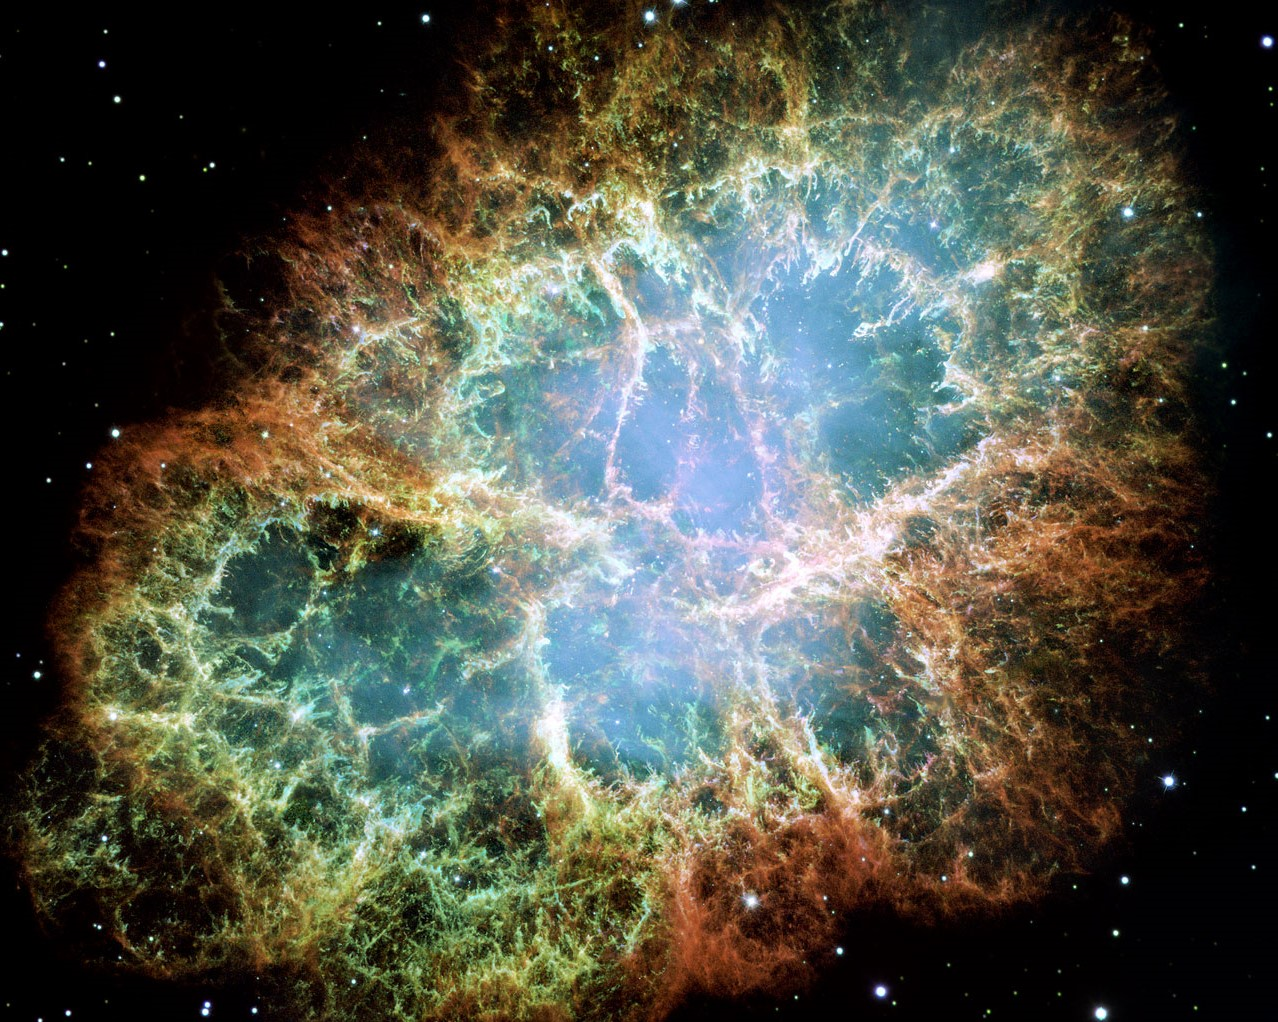
\includegraphics[width=\paperwidth, height =10cm]{../../Crab.jpg}}
    \end{figure}
\end{titlepage}

%%%%%%%%%%%%%%%%%%%%%%%
\tableofcontents

%%%%%%%%%%%%%%%%%%%%%%%%%%%%%%%%%%%%% Part 1
\part{Group Theory}

%%%%%%%%%%%%%%%%%%%%%% - P1.Chapter 1
\chapter{\textsection\textsection Basic Definitions and Examples: Groups}

\section{\textsection Initial Definitions}

\begin{defn}
    A \Emph{binary operation} on a non-empty set $S$ is a map $$\beta:S\times S\rightarrow S$$ where $S\times S := \{(a,b): a,b \in S\}$, and $(a,b)\mapsto a*b = \beta(a,b)$.
\end{defn}

\begin{eg}
    \leavevmode
    \begin{enumerate}
        \item $\map{S\times S\rightarrow S}{(a,b)\mapsto a}$ known as projection to the first factor
        \item $\map{\Z\times \Z\rightarrow \Z}{(a,b)\mapsto 0 = a*b}$ known as the zero map
        \item $\map{\Z\times \Z\rightarrow \Z}{(a,b)\mapsto a+b}$ addition
    \end{enumerate}
    \begin{rmk}
        There can be many different binary operations on a given set.
    \end{rmk}
\end{eg}

\begin{defn}[Group]
    A pair $(G, \star)$ where $G$ is a set and $\star$ is a binary operation on $G$ is called a \Emph{group} if: \begin{enumerate}
        \item[G1.] (\Emph{Associativity}) For all $a,b,c \in G$, $$(a\star b)\star c = a\star (b\star c)$$
        \item[G2.] (\Emph{Identity Element}) There exists $e \in G$ such that for all $a \in G$ $$a\star e = e \star a = a$$
        \item[G3.] (\Emph{Inverses}) For all $a \in G$ there exists $b \in G$ such that $$a \star b = b \star a = e$$ In this case we write $b = a^{-1}$
    \end{enumerate}
\end{defn}


\begin{rmk}
    The operation $\star$ can be denoted in many ways: $\cdot$, $+$, juxtaposition. The identity element $e$ is sometimes denoted $1_G$, $1$, $e_G$, and $0$.
\end{rmk}

\begin{eg}
    \leavevmode
    \begin{enumerate}
        \item $(\Z,+)$ is a group with $e = 0$ and the inverse of $a$ is denoted $-a$
        \item ($\R_{>0},\cdot$) where $\cdot$ is multiplication. $\cdot$ is a binary operation on $\R_{>0}$ because for all $a,b \in \R_{>0}$ we have $a,b >0$ so $a\cdot b > 0$ and $a \cdot b \in \R_{>0}$. Moreover, ($\R_{>0},\cdot$) is a group with identity $1$.
        \item (Non-example) $(\Z,-)$, $(a,b)\mapsto a-b$. This is not a group. Indeed, although $-$ is a binary operation on $\Z$, tere is no identity element and it's not associative.
        \item (Non-example) $(\Z\backslash \{0\},\cdot)$ is associative and has identity $1$, but does not have inverses for all $a \in \Z$.
    \end{enumerate}
\end{eg}

\begin{defn}
    A group $(G,\star)$ is called \Emph{abelian} if $a \star b = b \star a$ for all $a, b \in G$.
    \begin{rmk}
        Abelian groups are also known as \Emph{commutative groups}.
    \end{rmk}
\end{defn}


\begin{eg}
    $\GL_n(\R)$ is the general linear group of dimension $n \geq 1$, defined by \begin{equation}
        \GL_n(\R) := \left(\left\{ A \in M_{n\times n}(\R): \det(A) \neq 0\right\},\underbrace{\circ}_{matrix product}\right)
    \end{equation}
    \begin{xca}
        $\GL_n(\R)$ is a group with identity $I_n = (\delta_{ij})$, but it is non-abelian for $n \geq 2$.
    \end{xca}
\end{eg}

\begin{xca}
    If $(G,\star)$ is a group, then $(G,\star')$ is also group with $$a \star' b := b\star a, \forall a,b \in G$$
    \begin{proof}
        Note that for all $a,b \in G$, $a \star' b = b \star a \in G$ since $\star$ is a binary operation on $G$ by assumption, so $\star'$ is also a binary operation on $G$. (cont.)
    \end{proof}
\end{xca}


\section{\textsection The Group of Symmetries}

\begin{defn}[Symmetric Group]
    Let $X$ be a non-empty set. Then, define \begin{equation}
        S_X:=\{\sigma:X\rightarrow X:\sigma\;\text{is a bijection}\}
    \end{equation}
    Such a $\sigma$ is called a \Emph{permutation} of $X$. It follows that $(S_X, \circ)$ is a group where \begin{equation}
        \map{\circ:S_X\times S_X\rightarrow S_X}{(\sigma,\tau)\mapsto \sigma \circ \tau}
    \end{equation}
    is function composition. The group is also commonly denoted as $Sym(X)$.
    \begin{proof}
        Let $X$ be a non-empty set, and define $S_X$ as above. (cont.)
    \end{proof}
\end{defn}

\begin{defn}
    If $X = \{1,2,...,n\}$ for $n \in \N$, then $S_X = S_{\{1,2,...,n\}}$ is denoted $S_n$ and is called the \Emph{symmetric group of degree n} or \Emph{symmetric group on n letters}.
\end{defn}

\begin{eg}
    Take $n = 3$: $\sigma \in S_3$ can be represented as a $2\times n$ matrix by $$\begin{pmatrix} 1 & 2 & 3 \\ \sigma(1) & \sigma(2) & \sigma(3) \end{pmatrix}$$ where $\sigma(1)\;\sigma(2)\;\sigma(3)$ is a permutation of $1\;2\;3$.
    \begin{eg}
        $\sigma = \begin{pmatrix} 1 & 2 & 3 \\ 1 & 3 & 2 \end{pmatrix}$, $\gamma = \begin{pmatrix} 1 & 2 & 3 \\ 2 & 3 & 1 \end{pmatrix}$, then $$\sigma \circ \gamma = \begin{pmatrix} 1 & 2 & 3 \\ 3 & 2 & 1 \end{pmatrix}$$
        Observe $\sigma^{-1} = \begin{pmatrix} 1 & 2 & 3 \\ 1 & 3 & 2 \end{pmatrix} = \sigma$ and $\gamma^{-1} = \begin{pmatrix} 1 & 2 & 3 \\ 3 & 1 & 2 \end{pmatrix}$. 
    \end{eg}
    The identity permutation is denoted $\id = \begin{pmatrix} 1 & 2 & 3 \\ 1 & 2 & 3 \end{pmatrix}$
    \begin{note}
        We can also have written $$\begin{pmatrix} 2 & 1 & 3 \\ \sigma(2) & \sigma(1) & \sigma(3) \end{pmatrix}$$
        instead
    \end{note}
\end{eg}

\begin{eg}
    $n=2: S_2 = \{\id, \tau\}$, where $$\id = \begin{pmatrix} 1 & 2  \\ 1 & 2  \end{pmatrix}, \tau = \begin{pmatrix} 1 & 2 \\ 2 & 1 \end{pmatrix}, \tau^2 = \id$$
\end{eg}

\subsection{\textsection Notation: Cycles}

The cycle notation is more compact then the matrix-type notation, although this does come with some ambiguity:

\begin{eg}
    \leavevmode
    \begin{enumerate}
        \item $(1\;2) \in S_3$ means $1 \mapsto 2$, $2\mapsto 1$, and $3\mapsto 3$ (a \Emph{transposition}).
        \begin{enumerate}[label =\(\drsh\)]
            \item Note this is the same as $(2\;1)$ which is where ambiguity can arise.
        \end{enumerate}
        \item $(1\;2\;3) \in S_3$, means $1 \mapsto 2$, $2\mapsto 3$, $3\mapsto 1$
        \begin{enumerate}[label = $\drsh$]
            \item Visual - 
            \begin{tikzpicture}[->,scale=.7]
               \node (1) at (90:1cm)  {$1$};
               \node (2) at (-30:1cm) {$2$};
               \node (3) at (210:1cm) {$3$};
            
               \draw (70:1cm)  arc (70:-10:1cm);
               \draw (-50:1cm) arc (-50:-130:1cm);
               \draw (190:1cm) arc (190:110:1cm);
            \end{tikzpicture}
            (Note $(1\;2\;3) = (2\;3\;1) = (3\;1\;2)$)
        \end{enumerate}
    \end{enumerate}
\end{eg}


\begin{defn}
    Let $k_1,k_2,..., k_r \in \{1,2,...,n\}$ be distinct $(r \leq n)$. Then the permutation in $S_n$ which sends $k_1\mapsto k_2\mapsto k_3\mapsto ... \mapsto k_r \mapsto k_1$ and fixes all other numbers is denoted \begin{equation}
        (k_1\;k_2\;...\;k_r)
    \end{equation}
    which is a \Emph{cycle of length $r$} or an \Emph{$r$-cycle}.
\end{defn}

\begin{rmk}
    The only $1$-cycle is the identity permutation in $S_n$
    \begin{enumerate}
        \item[$\drsh$] $(1) = (2) = ... = (n)$
    \end{enumerate}
\end{rmk}

\begin{defn}
    Cycles of length $\geq 2$ in $S_n$ are called \Emph{disjoint} if they \emph{move} disjoint sets of numbers
    \begin{enumerate}
        \item[$\drsh$] \begin{eg}
            $(1\;2), (3\;4)$ are disjoint in $S_4$, but $(1\;2),(3\;1)$ are \underline{not}.
        \end{eg} 
    \end{enumerate}
\end{defn}


\begin{rmk}
    Every permutation in $S_n$($\neq \id$), can be written as a product of disjoint cycles of length $\geq 2$. Moreover, this factorization is unique up to the order of the factors.
    \begin{proof}
        (Left to the reader)
    \end{proof}
\end{rmk}

\begin{eg}
    In $S_5$ $(1\;4\;5)\circ(2\;3) = (2\;3) \circ(1\;4\;5)$ as they are disjoint
    \begin{enumerate}
        \item[$\drsh$] (so we can't hope for full unicity of the factorization) 
    \end{enumerate}
\end{eg}


\section{\textsection General Properties}

\begin{defn}
    For a group $(G, \star)$, the number of elements (cardinal) of $G$ is denoted $|G|$ and called the \Emph{order} of the group (can be infinite).
\end{defn}

\begin{eg}
    \begin{enumerate}
        \item $(\Z,+)$ has infinite order
        \item $(S_n,\circ)$ has order $n!$ (permutations)
    \end{enumerate}
\end{eg}

\begin{prop}
    Let $(G,\star)$ be a group. Then we have the following properties:
    \begin{enumerate}
        \item The identity element is unique.
        \begin{proof}
            If $e,i \in G$ are identity elements, then $e = e\star i = i$ as $e \star g = e$ and $g \star i = g$ for all $g \in G$ by assumption.
        \end{proof}
        \item The inverse of an element is unique.
        \begin{lem}[Cancellation Lemma]
            If $a \star b = a \star c$ or $b \star = c \star a$, then $b = c$ for all $a,b,c \in G$. 
        \end{lem}
        \begin{proof}
            Let $a^{-1}$ be an inverse of $a$. Then $$b = e\star b = (a^{-1} \star a) \star b = a^{-1} \star a \star c = e \star c = c$$ and similarly for $b \star a = c \star a$.
        \end{proof}
        \begin{rmk}
            $a \star b = c \star a$ does \underline{not} tell us anything in general.
        \end{rmk}
        \begin{proof}
            Take $b,c,$ inverses of $a$. Then $b \star a = e = c \star a$, so by the cancellation lemma $b = c$.
        \end{proof}
        \begin{enumerate}
            \item[$\drsh$] We will denote \underline{the} inverse of $a$ by $a^{-1}$ for all $a \in G$. 
        \end{enumerate}
        \begin{cor}
            For all $a \in G$, if $b \star a = e$ (or $a \star b = e$) the identity element, then we have that $b = a^{-1}$, so $b$ is the inverse of $a$.
        \end{cor}
    \end{enumerate}
\end{prop}


\begin{defn}
    Let $(G, \star)$ be a group. Let $n \in \Z$, $g \in G$, then \begin{equation}
        g^n = \left\{\begin{array}{ll} e, & \text{if } n = 0 \\ \underbrace{g\star g \star ... \star g}_{\text{n-fold times}}, & \text{if } n > 0 \\ \underbrace{g^{-1}\star g^{-1} \star ... \star g^{-1}}_{\text{-n-fold times}}, & \text{if } n < 0\end{array}\right.
    \end{equation}
\end{defn}

\begin{prop}
    For all $g \in G$ and all $n,m \in \Z$, \begin{enumerate}
        \item $(g^n)^m = g^{nm}$
        \item $g^n\star g^m = g^{n+m}$
    \end{enumerate}
    \begin{proof}
        (Left to the reader)
    \end{proof}
\end{prop}

\begin{eg}
    Let $G = \Z/2\Z$, $g = [1]$, and the operation be $+$. Then $g^{-1} = -1\cdot g = [-1] = [1]$, $g^0 = 0\cdot g = [0]$, $g^1 = 1\cdot g = [1]$, $g^2 = 2\cdot g = [1]+[1] = [2] = [0]$, and $g^3 = 3\cdot g = [3] = [1]$, etc.
\end{eg}

\begin{rmk}
    Due to associativity, the placement of parenthesis is unambiguous and unnecessary:
    $$\drsh ((a\star (b\star c)) \star d) = ((a \star b) \star (c \star d))$$
    Thus, $g_1\star g_2 \star ... \star g_n$ is well-defined for all $n \in \N$. 
    \begin{proof}
        (Left to the reader)
    \end{proof}
\end{rmk}

\begin{note}
    However, because we don't necessarily have commutivity, it is \underline{not} true in general that $(g\star h)^n = g^n \star h^n$. Indeed, $(g\star h )^2 = g\star h \star g \star h$, not necessarily $g^2\star h^2$.
\end{note}

\begin{rmk}[Inverse of a product]
    Let $a,b \in G$, a group. Then \begin{enumerate}
        \item $(a \star b)^{-1} = b^{-1}\star a^{-1}$
        \item More generally \begin{equation}
            (a_1\star a_2 \star ... \star a_n)^{-1} = a_n^{-1}\star ... \star a_2^{-1} \star a_1^{-1}
        \end{equation}
        for $a_i \in G$, $1 \leq i \leq n$
    \end{enumerate}
    \begin{proof}
        (Left to the reader)
    \end{proof}
\end{rmk}

\begin{eg}
    In $(\Z,+)$, $g^2$ for $g = 3$ is $g^2 = 2\cdot g = 2\cdot 3 = 6$. In general $g^n = ng$ for additive groups.
\end{eg}




%%%%%%%%%%%%%%%%%%%%%% - P1.Chapter 2
\chapter{\textsection\textsection Group Homomorphisms}

\section{\textsection Basic Definitions and Examples: Group Homomorphisms}

\begin{defn}[A]
    A \Emph{group homomorphism} from a group $A$ to a group $B$ is a map of sets $\phi:A\rightarrow B$ that satisfies the condition: \begin{equation}
        \forall a_1,a_2\in A,\;\;\;\phi(a_1\cdot a_2) = \phi(a_1)\cdot \phi(a_2)
    \end{equation}
    We can rewrite the condition on $\phi$ in terms of the requirement that the following diagram commute: \begin{center}
            \begin{tikzpicture}[baseline = (a).base]
            \node[scale = 1] (a) at (0,0){
                \begin{tikzcd}
                    A\times A  \ar[d, "\phi\times\phi", swap] \ar[r, "mult_A"] & A \ar[d,"\phi"] \\
                    B\times B \ar[r, "mult_B"] & B
                \end{tikzcd}
            };
            \end{tikzpicture}
        \end{center}
        We denote the set of all group homomorphisms from $A$ to $B$ by $\Hom_{\Grp}(A,B)$.
\end{defn}


\begin{defn}[B]
    Let $(G,\star)$ and $(M,\circ)$ be groups. A map $G\xrightarrow{f} M$ is a \Emph{homomorphism of groups} if \begin{equation}
        f(x\star y) = f(x)\circ f(y),\forall x,y \in G
    \end{equation} 
\end{defn}


\begin{eg}
    \leavevmode
    \begin{enumerate}
        \item $H \leq G$, then $H \xhookrightarrow{\iota} G$ the inclusion map is a \Emph{monomorphism} (an injective homomorphism)
        \item $\map{(\R,+)\rightarrow \R^{\times}}{x\mapsto 2^x}$ is a monomorphism.
        \item $\map{S_3 \hookrightarrow S_4}{\sigma \mapsto \sigma'}$, where $\sigma'(i) = \sigma(i)$ for $i \in \{1,2,3\}$ and $\sigma'(4) = 4$. In particular $$\begin{pmatrix} 1 & 2 & 3 \\ \sigma(1) & \sigma(2) & \sigma(3)  \end{pmatrix}\mapsto \begin{pmatrix} 1 & 2 & 3 & 4 \\ \sigma'(1) & \sigma'(2) & \sigma'(3) & 4  \end{pmatrix}$$
        is a monomorphism.
        \item $\map{\det:\GL_n(\R) \rightarrow \R^{\times}}{A \mapsto \det(A)}$ is an \Emph{epimorphism} (surjective homomorphism)
        \item $(G,\star)$ a group, then for $g \in G$, $$\map{\Z\xrightarrow{\phi_g}G}{x\mapsto g^n}$$ is a group homomorphism. It needs not be injective or surjective.
        \item $\map{|\cdot|:\C^{\times}\rightarrow \R^{\times}}{z\mapsto |Z|}$ is an epimorphism.
    \end{enumerate}
\end{eg}


\begin{props}
    Let $f:(G,\star)\rightarrow (H,\circ)$ be a group homomorphism. Then \begin{enumerate}
        \item $f(e_G) = e_H$
        \item for all $g \in G$, $f(g^{-1}) = (f(g))^{-1}$
        \item The composition of two homomorphisms $G \xrightarrow{f} H \xrightarrow{\phi}K$ is a homomorphism $G\xrightarrow{\phi \circ f}K$.
    \end{enumerate}
\end{props}
\begin{proof}
    (Left to the reader)
\end{proof}

\begin{rmk}
    \leavevmode
    \begin{enumerate}
        \item If $H_1 \leq G\xrightarrow{f} K$ where $f$ is a homomorphism, then the canonical map \begin{equation}
            f\rvert_{H_1}H_1\rightarrow K
        \end{equation}
        is a homomorphism called the \Emph{restriction of $f$ to $H_1$}. Moreover, $f\rvert_{H_1} = f \circ \iota_{H_1}$, where $\iota_{H_1}:H_1\hookrightarrow G$ is the inclusion homomorphism.
        \item Let $f:G\rightarrow K$ be a homomorphism. If the image of $f$, $\ran(f)$, is contained in a subgroup $H_2 \leq K$, then the associated map \begin{equation}
            f':G\rightarrow H_2
        \end{equation}
        is a homomorphism of groups.
    \end{enumerate}
\end{rmk}

\begin{eg}
    For $\det:\GL_n(\R)\rightarrow \R^{\times}$, we have $\SL_n(\R) \leq \GL_n(\R)$, so $\SL_n(\R)\xrightarrow{\det}\R^{\times}$ is a homomorphism, and \begin{equation}
        \ran\left(\det\rvert_{\SL_n(\R)}\right) = \{1\} \leq \R^{\times}
    \end{equation}
    so \begin{equation}
        \det:\SL_2(\R)\rightarrow \{1\}
    \end{equation}
    is a homomorphism.
\end{eg}


\begin{prop}
    Let $G\xrightarrow{f} K$ be a group homomorphism. Then \begin{enumerate}
        \item Let $H_1 \leq G$, then the image $f(H_1) \leq K$ is a subgroup of $K$
        \item Let $H_2 \leq K$, then $f^{-1}(H_2) \leq G$ is a subgroup of $G$, called the inverse image of $H_2$, or the pre-image of $H_2$ by $f$.
    \end{enumerate}
\end{prop}
\begin{proof}
    (Left to the reader)
\end{proof}


\begin{rmk}
        Note that the image of a cyclic subgroup $\langle g \rangle \leq G$ under a group homomorphism $f: G \rightarrow K$ is the cyclic subgroup \begin{equation}
                \langle f(g) \rangle \leq K
        \end{equation}
\end{rmk}
\begin{proof}
        (Left to the reader)
\end{proof}

\begin{cor}
        Let $G \xrightarrow{f} K$ be a group homomorphism. \begin{enumerate}
                \item The \Emph{image} $f(G) = \ran(f)$ is a subgroup of $K$
                \item The \Emph{kernel} $\ker(f) := f^{-1}(\{e_K\})$ is a subgroup of $G$
        \end{enumerate}
\end{cor}

\begin{prop}
        Let $G\xrightarrow{f} K$ be a group homomorphism. Then $f$ is injective (i.e. a \Emph{monomorphism}) if and only if $\ker(f) = \{e_G\}$.
\end{prop}
\begin{proof}
        (Left to the reader)
\end{proof}


\begin{eg}
        \leavevmode
        \begin{enumerate}
                \item $f$ a homomorphism is an isomorphism if and only if $\ker(f) = \{e_G\}$ and $\ran(f) = K$ (for $G\xrightarrow{f} K$)
                \item $H \leq G$, $H \xhookrightarrow{\iota} G$ the inclusion map is a homomorphism with $\ran(\iota) = H$ and $\ker(\iota) = \{e_G\}$
                \item The determinant map $\GL_n(\R)\xrightarrow{\det}\R^{\times}$ is a group homomorphism. Moroever, we obtain the subgroup \begin{equation}
                                \SL_n(\R) := \{A \in \GL_n(\R):\det(A) = 1\} = \ker(\det)
                        \end{equation}
                \item The map $\map{\Z\xrightarrow{\phi_g} G}{n \mapsto g^n}$ for some fixed $g \in G$ is a group homomorphism with image $\ran \phi_g = \langle g \rangle$, and $\ker(\phi_g) = \{n \in \Z:g^n = e_g\} = S_g$. Thus, $\phi_g$ is surjective if and only if $\langle g\rangle = G$ and $\phi_g$ is injective if and only if $o(g) = +\infty$.
                \item The modulus map $\C^{\times} \xrightarrow{|\cdot|}\R^{\times}$ is a group homomorphism with $\ker(|\cdot|) = \{z = \C^{\times}:|z| = 1\} = S^1$ the circle group, and $\ran(|\cdot|) = \R_{>0}$.
                \item The map $\map{\R\xrightarrow{\alpha}\C^{\times}}{\theta\mapsto \exp(2\pi i \theta)}$ is a group homomorphism with $\ker(\alpha) = \Z$ and $\ran(\alpha) = S^1$.
        \end{enumerate}
\end{eg}




\subsection{\textsection Group Isomorphisms}

\begin{eg}[motivating examples]
    \leavevmode
    \begin{enumerate}
        \item $g_1 := s_{\{1,2,3\}}$ and $g_2 := s_{\{a,b,c\}}$ are essentially the ``same" group, but their elements are not the same. indeed ``everything we do" in $g_1$ using the group operation we can do in $g_2$ by renaming $1$ as $a$, $2$ as $b$, and $3$ and $c$: order ($|g_1| = |g_2|$), subgroups, orders of elements, ``equations," etc.
        \item $\Z/2\Z = \{[0],[1]\}$, $g = \{+1,-1\} \leq (\R\backslash\{0\},\cdot) = \R^{\times}$ are the ``same" group. let us consider their \emph{cayley tables}:
        \begin{equation*}
            \begin{array}{c|cc}
                (\Z/2\Z,+) & [0] & {[1]}  \\ \hline
                {[0]} & [0] & {[1]} \\
                {[1]} & [1] & {[0]} \\
            \end{array}
            \hspace{40pt}
            \begin{array}{c|cc}
                (g, \cdot) & +1 & -1  \\ \hline
                +1 & +1 & -1 \\
                -1 & -1 & +1\\
            \end{array}
        \end{equation*}
        $[0]$ plays the role of $+1$ and $[1]$ plays the role of $-1$.
    \end{enumerate} 
\end{eg}



\begin{prop}
    $\Z/n\Z$ is isomorphic to the group of $n$th roots of unity: \begin{equation}
        \{z\in\C:z^n = 1\}
    \end{equation}
\end{prop}

\begin{defn}
    Let $(G,\star)$ and $(M,\circ)$ be groups. A bijective map $G\xrightarrow{f} M$ which is a group homomorphism is called an \Emph{isomorphism} of the groups $G$ and $M$. The groups $(G,\star)$ and $(M,\circ)$ are said to be \Emph{isomorphic}, denoted $(G,\star) \cong (M,\circ)$.
\end{defn}

\begin{eg}
    \leavevmode
    \begin{enumerate}
        \item $\map{\Z\xrightarrow{f}2\Z}{n\mapsto 2n}$ is a group isomorphism.
        \item If $G$ is a cyclic group, $G = \langle g \rangle$, and $|G| = n <+\infty$, then \begin{equation}
            \map{\Z/n\Z\xrightarrow{\phi}G}{{[m]}\mapsto g^m}
        \end{equation}
        is a group isomorphism. Recall that $g^m = g^{m'}$ if and only if $m\equiv m' \mod n$ ($o(g) = n$), so $\phi$ is well-defined and injective. By construction $\phi$ is also surjective. Therefore, $\Z/n\Z \cong G$.
        \item If $G = \langle g \rangle$ and $o(g) = +\infty$, then $G \cong \Z$. Indeed, the map \begin{equation}
            \map{\Z\xrightarrow{\phi} G}{m\mapsto g^m}
        \end{equation}
        is a group isomorphism.
        \item The map \begin{equation}
            \map{(\R,+)\xrightarrow{\exp}(\R_{>0},\cdot)}{x\mapsto e^x}
        \end{equation}
        is a group isomorphism, so $(\R,+)\cong (\R_{>0},\cdot)$. Another isomorphism is \begin{equation}
            \map{(\R,+)\xrightarrow{\phi}(\R_{>0},\cdot)}{x\mapsto 2^x}
        \end{equation}
        \item For all $h \in G$, where $(G,\star)$ is an arbitrary group, \begin{equation*}
            \map{(G,\star) \xrightarrow{\alpha_h}(G,\star)}{a \mapsto h^{-1}\star a \star h}
        \end{equation*}
        is a group isomorphism with inverse $\alpha_{h^{-1}}$.
        \item $\map{\Z\xrightarrow{\beta}\Z}{n\mapsto -n}$ is a group isomorphism.
    \end{enumerate}
\end{eg}

\begin{defn}
    An \Emph{isomorphism} $(G,\star)\rightarrow(G,\star)$ is called an \Emph{automorphism} of $(G,\star)$.
\end{defn}

\begin{prop}
    The set of automorphisms of a group $G$ is a subgroup of the symmetric group $S_G$.\begin{enumerate}
        \item The identity map $\map{\id:G\rightarrow G}{g\mapsto g}$ is an isomorphism (hence an automorphism) which acts as an identity for the group
        \item If $G\xrightarrow{\phi}H$ is an isomorphism, then the inverse $H\xrightarrow{\phi^{-1}}G$ is an isomorphism
        \item If $G\xrightarrow{\phi}H$ and $H\xrightarrow{\psi}K$ are isomorphisms, then the composition $\psi \circ \phi$ is also an isomorphism
    \end{enumerate}
\end{prop}
\begin{proof}
    (Left to the reader)
\end{proof}

\begin{cor}
    The set $\aut(G)$ of automorphisms of $G$ is a group for the composition of maps.
\end{cor}

\begin{eg}[Non-example]
    $\Q\cancel{\cong} \Q^{\times}$ because $-1 \in \Q^{\times}$ has order $2$, but $\Q$ does not have any element of order $2$. Indeed, if $x \in \Q$ such that $x+x=2x = 0$, then $x = 0$ so $o(x) = 1$. But, if $\Q^{\times}\xrightarrow{\phi}\Q$ is an isomorphism, then $o(\phi(-1)) = 2$, which is not possible.
\end{eg}

\begin{thm}[Dihedral Group Isomorphisms]
    Let $x,y \in G$ such that $G = \langle x,y \rangle (:= \langle \{x,y\}\rangle)$ with the relations $x^n = y^2 = e$, $yx = x^{-1}y$, and $n \geq 1$. Then $|G| \leq 2n$. If $|G| = 2n$, then the relation characterizes the group up to isomorphism.
\end{thm}
\begin{proof}
    If $n = 1$, $G \cong \Z/2\Z \cong D_1$. If $n = 2$, $G \cong \Z/2\Z \times \Z/2\Z \cong D_2$, mapping $x \mapsto ([1],[0])$ and $y \mapsto ([0],[1])$. Now, for all $n \geq 1$, let $Y_n := \{e,x,x^2,...,x^{n-1},y,xy,...,x^{n-1}y\}$. We know that $G = Y_n$ as sets from our study of the relations on the dihedral group. But $|Y_n| = 2n$ as a set, so $|G| \leq 2n$ as a group. If $|G| = 2n$, then all elements described in $Y_n$ are distinct in $G$, and the Caley table of the group is fixed by the relations. Thus, the group $G$ is uniquely determined up to isomorphism by the relations and $|G| = 2n$. If $n \geq 3$ we have seen that $\langle x = \phi_{2\pi/n},y = \psi_0\rangle = D_n$, $x,y$ satisfy the relations and $|D_n| = 2n$, so $G \rightarrow D_n$ is an isomorphism (taking $x$ in $G$ to $x$ in $D_n$ and $y$ in $G$ to $y$ in $D_n$).
\end{proof}

\begin{cor}
    $S_3 \cong D_3$ for $x = (1\;2\;3)$, $y = (1\;2)$.
    \begin{proof}
        (Left to the reader)
    \end{proof}
\end{cor}



\section{\textsection Automorphisms}

\begin{defn}
    Let $G$ be a group. An isomorphism from $G$ onto itself is called an \Emph{automorphism} of $G$. The group of all automorphisms on $G$ is denoted by $\aut(G)$.
\end{defn}


\begin{prop}
    Let $H$ be a normal subgroup of the group $G$. Then $G$ acts by conjugation on $H$ as automorphisms of $H$. More specifically, the action of $G$ on $H$ by conjugation is defined for each $g \in G$ by \begin{equation*}
        h\mapsto ghg^{-1}\;\;\;\text{ for each }\;h\in H
    \end{equation*}
    For each $g \in G$, conjugation by $g$ is an automorphism of $H$. The permutation representation afforded by this action is a homomorphisms of $G$ into $\aut(H)$ with kernel $C_G(H) = \{g \in G:\forall h\in H, ghg^{-1} =h\}$ (The centralizer of $H$ with respect to $G$). In particular, $G/C_G(H)$ is isomorphic to a subgroup of $\aut(H)$.
\end{prop}

\begin{rmk}
    This proposition implies that a group acts by conjugation on a normal subgroup as \emph{structure preserving permutations}, i.e. automorphisms.
\end{rmk}

\begin{cor}
    If $K$ is any subgroup of the group $G$ and $g \in G$, then $K \cong gKg^{-1}$. Conjugate elements and conjugate subgroups have the same order (as the induced map is an automorphism).
\end{cor}


\begin{cor}
    For any subgroup $H$ of a group $G$, the quotient group $N_G(H)/C_G(H)$ is isomorphic to a subgroup of $\aut(H)$. In particular, $G/Z(G)$ is isomorphic to a subgroup of $\aut(G)$.
\end{cor}
\begin{proof}
    Since $H$ is a normal subgroup of $N_G(H)$, our previous proposition implies that $N_G(H)$ acts by conjugation on $H$. Moreover, $C_G(H) \subseteq N_G(H)$, so the kernel of the permutation representation of $N_G(H)$ in $\aut(H)$ afforded by this action is $C_G(H)$. Hence by the first isomorphism theorem $N_G(H)/C_G(H)$ is isomorphic to a subgroup of $\aut(H)$.

    The second case follows from taking $H = G$, so $N_G(G) = G$ and $C_G(G) = Z(G)$.
\end{proof}


\begin{defn}
    Let $G$ be a group and let $g \in G$. Conjugation by $g$ is called an \Emph{inner automorphism} of $G$ and the subgroup of $\aut(G)$ consisting of all inner automorphisms is denoted by $\inn(G)$.
\end{defn}


\begin{defn}
    A subgroup $H$ of a group $G$ is called \Emph{characteristic in $G$} if and only if every automorphism of $G$ maps $H$ onto itself, i.e., $\sigma(H) = H$ for all $\sigma \in \aut(G)$.
\end{defn}


\begin{prop}
    Let $H$ be a subgroup of a group $G$: \begin{enumerate}
        \item If $H$ is characteristic in $G$ then $H \vartriangleleft G$,
        \item If $H$ is the unique subgroup of $G$ of a given order, then $H$ is characteristic in $G$,
        \item If $K$ is a characteristic subgroup of $H$ and $H \vartriangleleft G$, then $K\vartriangleleft G$.
    \end{enumerate}
\end{prop}
\begin{proof}
    (To be completed)
\end{proof}


\begin{cor}
    If $C$ is a cyclic group of order $n$, then every subgroup of $C$ is characteristic in $C$.
\end{cor}


\begin{prop}
    The automorphism group of the cyclic group of order $n$ is isomorphic to $(\Z/n\Z)^{\times}$, an abelian group of order $\varphi(n)$ (where $\varphi$ is the Euler-totient function).
\end{prop}
\begin{proof}
    Let $x$ be a generator of the cyclic group $\Z/n\Z$. If $\psi \in \aut(\Z/n\Z)$, then $\psi(x) = x^a$ for some $a \in \Z$, and the integer $a$ uniquely determines $\psi$. Denote this automorphism by $\psi_a$. As usual, since $|x| = n$, the integer $a$ is only defined modulo $n$. Since $\psi_a$ is an automorphism, $x$ and $x^a$ must have the same order, hence $\gcd(a,n) = 1$. Furthermore, for $a$ relatively prime to $n$, the map $x\mapsto x^a$ is an automorphism of $\Z/n\Z$. Hence we have a surjective map \begin{equation*}
        \map{\Psi:\aut(\Z/n\Z)\rightarrow (\Z/n\Z)^{\times}}{\psi_a\mapsto a\; (\mod n)}
    \end{equation*}
    The map $\Psi$ is a homomorphism because \begin{equation*}
        \psi_a\circ\psi_b(x) = \psi_a(x^b) = x^{ab} = \psi_{ab}(x)
    \end{equation*}
    for all $\psi_a,\psi_b \in \aut(\Z/n\Z)$, so that \begin{equation*}
        \Psi(\psi_a\circ\psi_b) = \Psi(\psi_{ab}) = ab\;(\mod n) = \Psi(\psi_a)\Psi(\psi_b)
    \end{equation*}
    Finally, $\Psi$ is injective by construction of the $\psi_a$, and hence is an isomorphism.
\end{proof}


\begin{eg}
    \leavevmode
    \begin{enumerate}
        \item If $p$ is an odd prime and $n \in \Z^+$, then the automorphism group of the cyclic group of order $p$ is cyclic of order $p-1$. More generally, the automorphism group of the cyclic group of order $p^n$ is cyclic of order $p^{n-1}(p-1)$.
        \item Let $p$ be a prime and let $V$ be an abelian group (written additively) with the property that $pv =0$ for all $v \in V$. If $|V| = p^n$, then $V$ is an $n$-dimensional vector space over the field $\F_p = \Z/p\Z$. The automorphisms of $V$ are precisely the non-singular linear transformations from $V$ to itself, that is \begin{equation*}
                \aut(V) \cong \GL(V) \cong \GL_n(\F_p)
        \end{equation*}
    \end{enumerate}
\end{eg}






%%%%%%%%%%%%%%%%%%%%%% - P1.Chapter 3
\chapter{\textsection\textsection Subgroups}

\section{\textsection Basic Definitions and Examples: Subgroups}

\begin{defn}
    A subset $H$ of a group $(G,\star)$ (i.e. $H \subseteq G$) is a \Emph{subgroup} if it satisfies the following properties:
    \begin{enumerate}
        \item[S1] (\Emph{identity}) $e \in H$, where $e$ is the identity in $G$ (so $H \neq \emptyset$)
        \item[S2] (\Emph{closure}) If $h_1,h_2 \in H$, then $h_1\star h_2 \in H$.
        \item[S3] (\Emph{inverses}) Of $h \in H$, then $h^{-1} \in H$.
    \end{enumerate}
    Thus, the group $(H,\star\vert_{H})$ makes sense. We denote this by $H \leq G$, to say $H$ is a subgroup of $G$ ($\star$ is understood from context)
\end{defn}

\begin{eg}
    \leavevmode
    \begin{enumerate}
        \item $\{e\} \leq G$ and $G \leq G$, for any group $G$. These subgroups are called the \Emph{trivial subgroups of $G$}.
        \item $\Z\leq \R$ with addition
        \item $l\Z := \{ln:n \in \Z\}\subset \Z$, where $l$ is fixed in $\Z$. $l\Z \leq \Z$. Indeed \begin{enumerate}
            \item[S1] $0 = l\cdot 0 \in l\Z$
            \item[S2] $ln+lm = l(n+m) \in l\Z$
            \item[S3] $ln + l(-n) = l(n+(-n)) = l\cdot 0 = 0$, so $-(ln) \in l\Z$.
        \end{enumerate}
        \item $SL_n(\R) := \{A \in Mat_n(\R):\det(A) = 1\} \leq \GL_2(\R)$ is a subgroup called the \Emph{special linear group} of degree $n$.
        \begin{proof}
            (Left to the reader)
        \end{proof}
        \item Let $S^1 := \{z \in \C:|z| = 1\}$, then $S^1 \leq \C\backslash\{0\} = \C^{\times}$, where the operation is multiplication. $S^1$ is called the \Emph{circle group}
    \end{enumerate}
\end{eg}


\begin{prop}
    If $H_1 \leq G$, $H_2 \leq G$ are subgroups of $G$, then $H = H_1 \cap H_2 \leq G$ is a subgroup.
    \begin{proof}
        (Left to the reader)
    \end{proof}
\end{prop}

\begin{cor}
    Let $\{H_{\alpha}\}_{\alpha \in J}$ be a collection of subgroups of a group $G$, where $J$ is an indexing set (possible infinite). Then \begin{equation}
        \bigcap_{\alpha \in J}H_{\alpha} \leq G
    \end{equation}
    \begin{proof}
        (Left to the reader)
    \end{proof}
\end{cor}

\subsection{\textsection Center}

\begin{defn}
    Let $(G,\star)$ be a group and let $g \in G$. The \Emph{centralizer} of $g \in G$ is \begin{equation}
        Z(g) := \{x \in G: \underbrace{x\star g = g \star x}_{x\text{ and }g\text{ commute}}\}
    \end{equation}
\end{defn}

\begin{claim}
    For all $g \in G$, for a group $(G,\star)$, $Z(g) \leq G$ is a subgroup of $G$.
    \begin{proof}
        (Left to the reader)
    \end{proof}
\end{claim}

\begin{eg}
    \leavevmode
    \begin{enumerate}
        \item $Z(2) \leq (\Z,+)$, and actually $Z(2) = \Z$ as $\Z$ is abelian.
        \item $Z(I_2 + E_{2,2}) \leq \GL_2(\R)$, and in particular $$Z(I_2+E_{2,2}) = \left\{\begin{pmatrix} a & 0 \\ 0 & d \end{pmatrix} \in \GL_2(\R):ad \neq 0, ad\in \R\right\}$$
    \end{enumerate}
\end{eg}

\begin{defn}
    The \Emph{center} $Z(G)$ of the group $G$ is \begin{equation}
        Z(G) := \{x \in G:x\star g = g \star x \forall g \in G\}
    \end{equation}
\end{defn}

\begin{prop}
    $Z(G) = \bigcap_{g \in G} Z(g)$, so also $Z(G) \leq G$.
\end{prop}

\begin{xca}
    For $n \geq 2$, $Z(\GL_n(\R)) \{aI_n: a \in \R^{\times}\}$
\end{xca}

\begin{rmk}
    For any group $G$, $Z(G)$ is an \Emph{abelian} group.
\end{rmk}


\section{\textsection Cyclic Subgroups}


\begin{defn}
    Let $S \subset G$ a subset of a group $G$. Then the \Emph{subgroup of $G$ generated by $S$} is \begin{equation}
        \langle S\rangle := \bigcap\{H \in \mathcal{P}(G): S \subset H \leq G\}
    \end{equation}
    (The intersection of all the subgroups of $G$ containing $S$) which is the smallest subgroup of $G$ containing $S$.
    \begin{note}
        $S \subset G \leq G$, so $S \subset \langle S \rangle$ and $\langle S \rangle$ is well-defined. $\langle S \rangle$ is the smallest subgroup of $G$ containing $S$ with respect to set inclusion.
    \end{note}
\end{defn}

\begin{eg}
    $\langle \emptyset\rangle = \{e\}$ and $\langle G \rangle = G$ (trivial subgroups)
\end{eg}

\begin{prop}
    Let $g \in G$, then \begin{equation}
        \langle \{g\}\rangle = \{g^n:n \in \Z\}
    \end{equation}
    and we write $\langle g \rangle := \langle \{g\}\rangle$.
    \begin{proof}
        (Left to the reader)
    \end{proof}
\end{prop}

\begin{eg}
    \leavevmode
    \begin{enumerate}
        \item $\langle e \rangle = \{e\}$
        \item For $[2] \in \Z/3\Z$, the $\langle [2] \rangle = \{[2], [1], [0]\} = \Z/3\Z$.
        \item For $l \in \Z$, $\langle l \rangle = \{nl:n\in\Z\}\leq \Z$. We write $l\Z := \langle l \rangle$.
    \end{enumerate}
\end{eg}

\begin{defn}
    A group $K$ such that there exists $g \in K$ with $\langle g \rangle = K$ is called a \Emph{cyclic group}.
\end{defn}
\begin{enumerate}
    \item[$\drsh$] i.e$\rangle$ A group generated by single element is called \Emph{cyclic}.
\end{enumerate}


\begin{defn}
    Then, for all $g \in G$, $\langle g \rangle \leq G$ is cyclic. The order of $|\langle g \rangle|$ of the group $\langle g \rangle$ is called the \Emph{order of $g$}, and denoted $o(g)$ (could be infinite!).
\end{defn}


\begin{eg}
    \leavevmode
    \begin{enumerate}
        \item For $1 \in \Z$, $o(1) = \infty$ given $\langle 1 \rangle = \Z$. Thus, $\Z$ is cyclic of infinite order.
        \begin{enumerate}
            \item[$\drsh$] \underline{Note:} The \underline{only} other generator of $\Z$ is $-1$.
            \begin{enumerate}
                \item[$\drsh$] For $2 \in \Z$ does not generate $\Z$ because $\langle 2 \rangle = 2\Z \subsetneq \Z$ 
            \end{enumerate}
        \end{enumerate}
        \item For $n \in \Z_{>0}$, $[1]_n \in \Z/n\Z$, $o([1]_n) = n$ given $$\langle [1]_n\rangle = \{k[1]_n:k \in \Z\} = \Z/n\Z$$
        Thus $\Z/n|Z$ is a cyclic group of order $n$.
        \item For any group $G$, $o(e) = 1$ where $e$ is the identity of $G$.
        \item $\Q^{\times} = (\Q\backslash\{0\},\cdot)$ is not cyclic.
        \begin{proof}
            Assume $\Q^{\times} = \langle \frac{a}{b}\rangle$, then take $p$ relatively prime to $a$ and to $p$. Then $p \notin \left\{\left(\frac{a}{b}\right)^n: n \in \Z\right\}$, which contradicts the assumption and $\Q^{\times}$ is not cyclic.
        \end{proof}
    \end{enumerate}
\end{eg}


\begin{rmk}
    A cyclic group is abelian.
    \begin{proof}
        (Left to the reader)
    \end{proof}
\end{rmk}

\begin{cor}
    If a group is non-abelian it cannot be cyclic.
    \begin{proof}
        Contrapositive of the previous statement.
    \end{proof}
\end{cor}
\begin{enumerate}
    \item[$\drsh$] $\GL_n(\R)$, $n \geq 2$, and $S_m$, $m \geq 3$, are not cyclic as they are non-abelian. 
\end{enumerate}


$\Z$ is cyclic and properties of $\Z$ will have consequences for all cyclic groups (through isomorphisms).

\begin{thm}
    Every subgroup $H$ of $(\Z,+)$ is of the form $n\Z = \langle n \rangle$ for some $n \in \Z$.
    \begin{proof}
        (Left to the reader)
    \end{proof}
\end{thm}

\begin{cor}[GCD]
    Let $a,b \in \Z$ and define \begin{equation}
        a\Z + b\Z := \{an + bm: n,m \in \Z\} \subset \Z
    \end{equation}
    $a\Z+b\Z$ is a subgroup of $(\Z,+)$ generated by $\{a,b\}$. Then, by the previous theorem $a\Z + b\Z = d\Z$ for some $d \in \Z$, and if $(a,b) \neq (0,0)$, we have that $d = \gcd(a,b)$. We choose $d > 0$ to maintain uniqueness.
    \begin{proof}
        (Left to the reader)
    \end{proof}
\end{cor}

\begin{cor}
    Suppose $a\Z + b\Z = d\Z$, $(a,b) \neq (0,0)$, so $d \neq 0$. Then \begin{enumerate}
        \item $d\;\vert\;a$ and $d\;\vert\;b$.
        \item If $e \;\vert\;a$ and $e\;\vert\;b$, then $e \;\vert\;d$.
        \item There exist $x,y \in \Z$ such that $d = ax + by$.
    \end{enumerate}
\end{cor}

\begin{prop}
    Take the cyclic subgroup $\langle g \rangle \leq G$ of $G$. Then define \begin{equation}
        S_g := \{k \in \Z: g^k = e\}\subset \Z
    \end{equation}
    It follows that \begin{enumerate}
        \item $S_g \leq \Z$ is a subgroup for all $g \in G$.
        \item For $r,s \in \Z$, $g^r = g^s$ if and only if $r-s \in S_g$.
        \item If $S_g \neq \{0\}$, then $S_g = n\Z$ for some $n >0$, and \begin{equation}
            \langle g \rangle = \{e,g,g^2,...,g^{n-1}\}
        \end{equation}
        with $o(g) =n$.
        \item $S_g = \{0\}$ if and only if $o(g) = \infty$, in which case $g^m = g^n$ if an only if $m = n$.
        \item The order of $g^l$ is $\frac{n}{\gcd(l,n)}$ if $o(g) = n$.
    \end{enumerate}
\end{prop}
\begin{proof}
    (Left to the reader)
\end{proof}

\begin{rmk}
    If $o(g) = \infty$, $g^r = g^s$ if and only if $r = s$. If $o(g) = n < \infty$, $g^r = g^s$ if and only if $r \equiv s \mod n$.
    \begin{enumerate}
        \item[$\drsh$] $o(g)$ is the smallest integer $n > 0$ such that $g^n = e$. (If $\cancel{\exists}n > 0$ such that $g^n = e$, then $o(g) = \infty$) 
    \end{enumerate}
\end{rmk}

\begin{cor}
    For $g \in G$, $g^l$ is a generator of $\langle g \rangle$ if and only if $\gcd(l,n) = 1$, where $n = o(g)$.
\end{cor}
\begin{enumerate}
    \item[$\drsh$] If $o(g) = \infty$ then $\langle g^l \rangle = \langle g \rangle$ if and only if $l \in \{1,-1\}$
\end{enumerate}
\begin{proof}
    (Left to the reader)
\end{proof}

\begin{thm}
    Every subgroup of a cyclic group is itself cyclic.
    \begin{proof}
        (Left to the reader)
    \end{proof}
\end{thm}

\begin{eg}
    \leavevmode
    \begin{enumerate}
        \item For $2 \in (
        \Z,+)$, $o(2) = \infty$, so $\langle 2 \rangle = 2\Z$, and $|2\Z| = \infty$.
        \item For $[2] \in \Z/3\Z$, $o([2]) = 3$, so $\langle [2]\rangle = \Z/3\Z$. Indeed, $\langle [1]\rangle = \Z/3\Z$, so $$o([2]) = o(2[1]) = \frac{o([1])}{\gcd(o([1]),2)} = \frac{3}{\gcd(3,2)} = 3$$
        \item For $[2] \in \Z/4\Z$, $o([2]) = 2$, so $\langle [2] \rangle < \Z/4\Z$ is a proper subgroup.
    \end{enumerate}
\end{eg}


\begin{cor}
        Let $G = \langle g \rangle$ be cyclic. Then every subgroup of $G$ is cyclic.
\end{cor}
\begin{proof}
        Consider the epimorphism \begin{equation}
                \map{\Z\xrightarrow{\phi_g}G}{n\mapsto g^n}
        \end{equation}
        Let $H \subseteq G$. Then $\phi^{-1}_g(H) = H' \subseteq \Z$ because of the properties of the inverse images of subgroups under group homomorphisms. Thus since $\phi_g$ is cyclic, $\phi_g(H') = H$, so $H$ is the image of a subgroup $H'$ of $\Z$. But, all subgroups of $\Z$ are cyclic. Thus $\phi_g(H')$ is cyclic since it is the image of a cyclic subgroup under a group homomorphism.
\end{proof}


\begin{thm}
        If $G$ is a cyclic group of order $n < +\infty$, then the order of every subgroup $H$ of $G$ divides $n$. Moreover, for every divisor $q$ of $n$, there exists a unique subgroup of $G$ of order $q$.
\end{thm}
\begin{proof}
        Let $G = \langle g \rangle$, $H \subseteq G$, and $o(g) = n$. By the previous corollary $H = \langle g^l \rangle$ for some $l \geq 0$. It follows that $|H| = \frac{n}{\gcd(n,l)}$. Thus, $$\frac{n}{\gcd(n,l)} = |H|\;\vert\;|G| = n$$ Suppose $|H| = |H'| (=\langle g^{l'}\rangle)$, so $\gcd(l,n) = \gcd(l',n)$. Note that $o(g^{\gcd(l,n)}) = \frac{n}{\gcd(n,\gcd(l,n))} = \frac{n}{\gcd(n,l)} = o(g^l)$ and since $\gcd(l,n)\;\vert\;l$ $g^l \in \langle g^{\gcd(l,n)}\rangle$. Hence, we have that \begin{equation}
                H = \langle g^l \rangle = \langle g^{\gcd(l,n)} \rangle = \langle g^{\gcd(l',n)} \rangle = \langle g^{l'} \rangle = H'
        \end{equation}
        Thus we have uniqueness, and that the order of any subgroup must divide that of the group. For existence, suppose $n = qr$ for some integer $r$. Then $H = \langle g^r\rangle$ is a subgroup of order $$|H| = o(g^r) = \frac{n}{\gcd(n,r)} = \frac{qr}{r} = q$$ satisfying existence.
\end{proof}



\section{\textsection Dihedral Groups}

\begin{claim}
    If $S$ is a non-empty subset of $G$, then \begin{equation}
        \langle S\rangle = \{s_1^{k_1}\star s_2^{k_2} \star ... \star s_m^{k_m}: m\geq 1, s_1,s_2,...,s_m \in S,k_1,k_2,...,k_m\in\Z\}
    \end{equation}
    Or, equivalently \begin{equation}
        \langle S\rangle = \{r_1^{\alpha_1}\star r_2^{\alpha_2} \star ... \star r_n^{\alpha_n}: n\geq 1, r_1,r_2,...,r_n \in S,\alpha_1,\alpha_2,...,\alpha_n\in\{1,-1\}\}
    \end{equation}
\end{claim}

\begin{rmk}
    The $s_i$'s (and $r_i$'s) in these two descriptions need not be distinct. This is a generalization of the description of $\langle g \rangle$. This is by no means a unique way to write elements of $\langle S\rangle$.
\end{rmk}

\begin{eg}
    For $S = \{a,b\}$, \begin{enumerate}
        \item If $a \star b = b \star a$, for all $m \geq 1$, \begin{equation}
            s_1^{k_1}\star s_2^{k_2} \star ... \star s_m^{k_m} = a^k \star b^l
        \end{equation}
        \item In additive notation we get $a^k \star b^l = ka + lb$, so $\langle \{a,b\}\rangle = \Z a + \Z b$. (In general this need not be cyclic)
    \end{enumerate}
\end{eg}

\begin{rmk}
    If we don't assume $a \star b = b \star a$, then we cannot simplify a general element to the form $a^k \star b^l$ in $\langle S \rangle$.
\end{rmk}


\begin{defn}
    A polygon $X$ is \Emph{regular} if it is \Emph{equiangular} (all angles are equal in measure) and \Emph{equilateral} (all sides have the same length).
\end{defn}
\begin{enumerate}
    \item[$\drsh$] \begin{note}
        The vertices of such a figure (if it is convex) can always be drawn on a circle called the \Emph{circumcircle}.
    \end{note} 
\end{enumerate}

\begin{eg}
    \leavevmode
    \begin{enumerate}
        \item $3$-sides $=$ equilateral triangle: \begin{center}
            \begin{tikzpicture}[x=0.75pt,y=0.75pt,yscale=-1,xscale=1]
            %uncomment if require: \path (0,300); %set diagram left start at 0, and has height of 300
            
            %Shape: Circle [id:dp6369909468365647] 
            \draw   (66.67,160.5) .. controls (66.67,111.44) and (106.44,71.67) .. (155.5,71.67) .. controls (204.56,71.67) and (244.33,111.44) .. (244.33,160.5) .. controls (244.33,209.56) and (204.56,249.33) .. (155.5,249.33) .. controls (106.44,249.33) and (66.67,209.56) .. (66.67,160.5) -- cycle ;
            %Shape: Triangle [id:dp2358003807310185] 
            \draw   (155.83,71) -- (235.5,200) -- (75.67,200) -- cycle ;
            
            
            
            \draw [fill={rgb, 255:red, 3; green, 3; blue, 3 }  ,fill opacity=1 ]  (156.25, 71.67) circle [x radius= 2, y radius= 2]   ;
            \draw [fill={rgb, 255:red, 3; green, 3; blue, 3 }  ,fill opacity=1 ]  (235.27, 199.63) circle [x radius= 2, y radius= 2]   ;
            \draw [fill={rgb, 255:red, 3; green, 3; blue, 3 }  ,fill opacity=1 ]  (235.09, 200) circle [x radius= 2, y radius= 2]   ;
            \draw [fill={rgb, 255:red, 3; green, 3; blue, 3 }  ,fill opacity=1 ]  (75.91, 200) circle [x radius= 2, y radius= 2]   ;
            \draw [fill={rgb, 255:red, 3; green, 3; blue, 3 }  ,fill opacity=1 ]  (155.42, 71.67) circle [x radius= 2, y radius= 2]   ;
            \draw [fill={rgb, 255:red, 3; green, 3; blue, 3 }  ,fill opacity=1 ]  (75.8, 199.78) circle [x radius= 2, y radius= 2]   ;
            \end{tikzpicture}
        \end{center}
        \item $4$-sides $=$ square 
        \begin{center}
            \begin{tikzpicture}[x=0.75pt,y=0.75pt,yscale=-1,xscale=1]
            %uncomment if require: \path (0,300); %set diagram left start at 0, and has height of 300
            
            %Shape: Circle [id:dp6369909468365647] 
            \draw   (66.67,160.5) .. controls (66.67,111.44) and (106.44,71.67) .. (155.5,71.67) .. controls (204.56,71.67) and (244.33,111.44) .. (244.33,160.5) .. controls (244.33,209.56) and (204.56,249.33) .. (155.5,249.33) .. controls (106.44,249.33) and (66.67,209.56) .. (66.67,160.5) -- cycle ;
            %Shape: Square [id:dp9411752355047514] 
            \draw   (92.4,97.4) -- (218.6,97.4) -- (218.6,223.6) -- (92.4,223.6) -- cycle ;
            
            
            
            \draw [fill={rgb, 255:red, 3; green, 3; blue, 3 }  ,fill opacity=1 ]  (92.97, 97.4) circle [x radius= 2, y radius= 2]   ;
            \draw [fill={rgb, 255:red, 3; green, 3; blue, 3 }  ,fill opacity=1 ]  (218.03, 97.4) circle [x radius= 2, y radius= 2]   ;
            \draw [fill={rgb, 255:red, 3; green, 3; blue, 3 }  ,fill opacity=1 ]  (218.6, 97.97) circle [x radius= 2, y radius= 2]   ;
            \draw [fill={rgb, 255:red, 3; green, 3; blue, 3 }  ,fill opacity=1 ]  (218.6, 223.03) circle [x radius= 2, y radius= 2]   ;
            \draw [fill={rgb, 255:red, 3; green, 3; blue, 3 }  ,fill opacity=1 ]  (218.03, 223.6) circle [x radius= 2, y radius= 2]   ;
            \draw [fill={rgb, 255:red, 3; green, 3; blue, 3 }  ,fill opacity=1 ]  (92.97, 223.6) circle [x radius= 2, y radius= 2]   ;
            \draw [fill={rgb, 255:red, 3; green, 3; blue, 3 }  ,fill opacity=1 ]  (92.4, 97.97) circle [x radius= 2, y radius= 2]   ;
            \draw [fill={rgb, 255:red, 3; green, 3; blue, 3 }  ,fill opacity=1 ]  (92.4, 223.03) circle [x radius= 2, y radius= 2]   ;
            \end{tikzpicture}
        \end{center}
        \item $5$-sides $=$ pentagon
        \begin{center}
            \begin{tikzpicture}[x=0.75pt,y=0.75pt,yscale=-1,xscale=1]
            %uncomment if require: \path (0,300); %set diagram left start at 0, and has height of 300
            
            %Shape: Circle [id:dp6369909468365647] 
            \draw   (66.67,160.5) .. controls (66.67,111.44) and (106.44,71.67) .. (155.5,71.67) .. controls (204.56,71.67) and (244.33,111.44) .. (244.33,160.5) .. controls (244.33,209.56) and (204.56,249.33) .. (155.5,249.33) .. controls (106.44,249.33) and (66.67,209.56) .. (66.67,160.5) -- cycle ;
            %Shape: Regular Polygon [id:dp6960584174528508] 
            \draw   (239.03,131.12) -- (209.26,230.86) -- (105.19,233.37) -- (70.65,135.17) -- (153.37,71.98) -- cycle ;
            
            
            
            
            \end{tikzpicture}
        \end{center}
        \item $n$-sides $=$ regular convex $n$-gon
        \begin{center}
            \begin{tikzpicture}[x=0.75pt,y=0.75pt,yscale=-1,xscale=1]
            %uncomment if require: \path (0,300); %set diagram left start at 0, and has height of 300
            
            %Shape: Circle [id:dp6369909468365647] 
            \draw   (66.67,160.5) .. controls (66.67,111.44) and (106.44,71.67) .. (155.5,71.67) .. controls (204.56,71.67) and (244.33,111.44) .. (244.33,160.5) .. controls (244.33,209.56) and (204.56,249.33) .. (155.5,249.33) .. controls (106.44,249.33) and (66.67,209.56) .. (66.67,160.5) -- cycle ;
            %Shape: Regular Polygon [id:dp6960584174528508] 
            \draw   (239.03,131.12) -- (240.35,185.83) -- (209.26,230.86) -- (157.63,249.02) -- (105.19,233.37) -- (71.97,189.88) -- (70.65,135.17) -- (101.74,90.14) -- (153.37,71.98) -- (205.81,87.63) -- cycle ;
            
            
            
            
            \end{tikzpicture}
        \end{center}
    \end{enumerate}
\end{eg}


\begin{defn}
    Let $n \geq 3$. The \Emph{dihedral group} $D_n$ is the \Emph{symmetry group} of the regular convex $n$-gon. Consider the following maps $\R^2 \rightarrow \R^2$:\begin{enumerate}
        \item For all $\alpha \in \R$, $\phi_{\alpha}$ is the rotation about the origin of $|R^2$ of angle $\alpha$ radians.
        \item For all $\alpha \in \R$, $\psi_{\alpha}$ is the reflection with respect to a line $l_{\alpha}$ going through the origin and forming an angle $\alpha$ radians with the $x$-axis:
        \begin{center}
            \begin{tikzpicture}[x=0.75pt,y=0.75pt,yscale=-1,xscale=1]
            %uncomment if require: \path (0,300); %set diagram left start at 0, and has height of 300
            
            \draw   (-1,170.8) -- (277.83,170.8)(138.42,89.2) -- (138.42,252.4) ;
            %Straight Lines [id:da1735016350905001] 
            \draw    (35.2,212.4) -- (245.35,125.56) ;
            \draw [shift={(247.2,124.8)}, rotate = 517.55] [color={rgb, 255:red, 0; green, 0; blue, 0 }  ][line width=0.75]    (10.93,-3.29) .. controls (6.95,-1.4) and (3.31,-0.3) .. (0,0) .. controls (3.31,0.3) and (6.95,1.4) .. (10.93,3.29)   ;
            %Shape: Arc [id:dp5422827964833219] 
            \draw  [draw opacity=0] (161.34,160.12) .. controls (163.99,162.87) and (165.6,166.46) .. (165.6,170.4) .. controls (165.6,170.48) and (165.6,170.55) .. (165.6,170.63) -- (148.4,170.4) -- cycle ; \draw   (161.34,160.12) .. controls (163.99,162.87) and (165.6,166.46) .. (165.6,170.4) .. controls (165.6,170.48) and (165.6,170.55) .. (165.6,170.63) ;
            \draw   (273.83,166.67) -- (278.17,170.58) -- (273.83,174.5) ;
            \draw   (134.42,93.1) -- (138.33,88.75) -- (142.26,93.07) ;
            
            % Text Node
            \draw (237.83,113.73) node [anchor=north west][inner sep=0.75pt]  [font=\tiny]  {$l_{\alpha }$};
            % Text Node
            \draw (169.5,160.4) node [anchor=north west][inner sep=0.75pt]  [font=\tiny]  {$\alpha $};
            
            
            \end{tikzpicture}
        \end{center}
    \end{enumerate}
\end{defn}

\begin{claim}
    For all $\alpha,\beta \in \R$, \begin{enumerate}
        \item $\phi_{\alpha} \circ \phi_{\beta} = \phi_{\alpha + \beta}$ (rotation) 
        \item $\psi_{\alpha} \circ \psi_{\beta} = \phi_{2(\alpha - \beta)}$ (rotation) 
        \item $\phi_{\alpha} \circ \psi_{\beta} = \psi_{\beta + \frac{1}{2}\alpha}$ (reflection) 
        \item $\psi_{\beta} \circ \phi_{\alpha} = \psi_{\beta - \frac{1}{2}\alpha}$ (reflection) 
    \end{enumerate}
    \begin{enumerate}
        \item[$\drsh$] (Where $\circ$ is the composition of maps $\R^2\rightarrow \R^2$). 
    \end{enumerate}
\end{claim}

\begin{note}
    This is \underline{not} commutative.
\end{note}


\begin{cor}
    The composition of maps induces a binary operation on the set of rigid motions and reflections about the origin, $\R^2\rightarrow \R^2$.
\end{cor}

\begin{prop}
    This set is a group with \begin{equation}
        \phi_{\alpha}^{-1} = \phi_{-\alpha}, \psi^{-1}_{\beta} = \psi_{\beta}, \;\text{and}\;\phi_0 = \id
    \end{equation}
    for all $\alpha,\beta \in \R$. Moreover, since $\circ$ is associative, it is indeed a group.
\end{prop}

\begin{defn}
    This group is called the \Emph{orthogonal group}, $O_2(\R)$.
\end{defn}

\begin{prop}
    Note that $O_2(\R) \leq \GL_2(\R)$ since the maps are linear. Indeed: \begin{equation}
        \phi_{\alpha} = \begin{bmatrix} \cos\alpha & -\sin\alpha \\ \sin\alpha & \cos\alpha \end{bmatrix}, \psi_{\alpha} = \begin{bmatrix} \cos2\alpha & \sin2\alpha \\ \sin2\alpha & -\cos2\alpha \end{bmatrix}, 
    \end{equation}
    in the standard basis of $\R^2$.
\end{prop}

\begin{defn}
    Let $N \geq 3$, the $n$-th \Emph{dihedral group $D_n$} is the subgroup of $O_2(\R)$ preserving a regular $n$-gon $X_n$ with a circumcircle centered at the origin of $\R^2$:\begin{equation}
        D_n := \{f \in O_2(\R): f(X_n) = X_n\}
    \end{equation}
\end{defn}

\begin{eg}
    For $n =6$ we have \begin{center}
        \begin{tikzpicture}[x=0.75pt,y=0.75pt,yscale=-1,xscale=1]
        %uncomment if require: \path (0,300); %set diagram left start at 0, and has height of 300
        
        %Shape: Circle [id:dp6369909468365647] 
        \draw   (66.67,160.5) .. controls (66.67,111.44) and (106.44,71.67) .. (155.5,71.67) .. controls (204.56,71.67) and (244.33,111.44) .. (244.33,160.5) .. controls (244.33,209.56) and (204.56,249.33) .. (155.5,249.33) .. controls (106.44,249.33) and (66.67,209.56) .. (66.67,160.5) -- cycle ;
        %Shape: Regular Polygon [id:dp6960584174528508] 
        \draw   (243.76,160.65) -- (199.42,237.3) -- (110.87,237.22) -- (66.67,160.5) -- (111.01,83.85) -- (199.55,83.93) -- cycle ;
        \draw   (49,161.13) -- (261.5,161.13)(155.25,65) -- (155.25,257.25) ;
        %Straight Lines [id:da00457972531911599] 
        \draw    (57,102.75) -- (259.5,222.5) ;
        %Straight Lines [id:da41124966975132526] 
        \draw    (49.5,227.25) -- (251,101.75) ;
        %Straight Lines [id:da32514486377192964] 
        \draw    (95.5,56.75) -- (219.5,271.25) ;
        %Straight Lines [id:da39830526708721803] 
        \draw    (211.5,65.75) -- (93,267.25) ;
        %Shape: Arc [id:dp7870194689907395] 
        \draw  [draw opacity=0] (183.31,146.13) .. controls (186.15,150.43) and (187.91,155.5) .. (188.2,160.96) -- (158.25,162.63) -- cycle ; \draw   (183.31,146.13) .. controls (186.15,150.43) and (187.91,155.5) .. (188.2,160.96) ;
        \draw   (183.75,151.63) -- (182.82,146.15) -- (188.37,145.84) ;
        
        % Text Node
        \draw (191.5,148.4) node [anchor=north west][inner sep=0.75pt]  [font=\tiny]  {$\alpha $};
        
        \draw [fill={rgb, 255:red, 3; green, 3; blue, 3 }  ,fill opacity=1 ]  (200.75, 84.04) circle [x radius= 2, y radius= 2]   ;
        \draw [fill={rgb, 255:red, 3; green, 3; blue, 3 }  ,fill opacity=1 ]  (110.67, 237.21) circle [x radius= 2, y radius= 2]   ;
        \draw [fill={rgb, 255:red, 3; green, 3; blue, 3 }  ,fill opacity=1 ]  (110.77, 237.04) circle [x radius= 2, y radius= 2]   ;
        \draw [fill={rgb, 255:red, 3; green, 3; blue, 3 }  ,fill opacity=1 ]  (200.17, 85.01) circle [x radius= 2, y radius= 2]   ;
        \draw [fill={rgb, 255:red, 3; green, 3; blue, 3 }  ,fill opacity=1 ]  (155.41, 161.13) circle [x radius= 2, y radius= 2]   ;
        \draw [fill={rgb, 255:red, 3; green, 3; blue, 3 }  ,fill opacity=1 ]  (155.25, 161.4) circle [x radius= 2, y radius= 2]   ;
        \draw [fill={rgb, 255:red, 3; green, 3; blue, 3 }  ,fill opacity=1 ]  (155.49, 160.99) circle [x radius= 2, y radius= 2]   ;
        \draw [fill={rgb, 255:red, 3; green, 3; blue, 3 }  ,fill opacity=1 ]  (155.26, 161.38) circle [x radius= 2, y radius= 2]   ;
        \draw [fill={rgb, 255:red, 3; green, 3; blue, 3 }  ,fill opacity=1 ]  (155.63, 160.76) circle [x radius= 2, y radius= 2]   ;
        \draw [fill={rgb, 255:red, 3; green, 3; blue, 3 }  ,fill opacity=1 ]  (111.02, 83.59) circle [x radius= 2, y radius= 2]   ;
        \draw [fill={rgb, 255:red, 3; green, 3; blue, 3 }  ,fill opacity=1 ]  (199.95, 237.43) circle [x radius= 2, y radius= 2]   ;
        \draw [fill={rgb, 255:red, 3; green, 3; blue, 3 }  ,fill opacity=1 ]  (199.65, 236.91) circle [x radius= 2, y radius= 2]   ;
        \draw [fill={rgb, 255:red, 3; green, 3; blue, 3 }  ,fill opacity=1 ]  (111.17, 83.85) circle [x radius= 2, y radius= 2]   ;
        \draw [fill={rgb, 255:red, 3; green, 3; blue, 3 }  ,fill opacity=1 ]  (155.84, 161.13) circle [x radius= 2, y radius= 2]   ;
        \draw [fill={rgb, 255:red, 3; green, 3; blue, 3 }  ,fill opacity=1 ]  (155.25, 160.11) circle [x radius= 2, y radius= 2]   ;
        \draw [fill={rgb, 255:red, 3; green, 3; blue, 3 }  ,fill opacity=1 ]  (155.9, 161.24) circle [x radius= 2, y radius= 2]   ;
        \draw [fill={rgb, 255:red, 3; green, 3; blue, 3 }  ,fill opacity=1 ]  (155.79, 161.05) circle [x radius= 2, y radius= 2]   ;
        \end{tikzpicture}
    \end{center}
    We have $6$-rotations $$\{\phi_{2\pi/6},\phi_{4\pi/6},\phi_{6\pi/6},\phi_{8\pi/6},\phi_{10\pi/6},\phi_{12\pi/6}\}$$ and $6$-reflections $$\{\psi_{\pi/6},\psi_{2\pi/6},\psi_{3\pi/6},\psi_{4\pi/6},\psi_{5\pi/6},\psi_{6\pi/6}\}$$
\end{eg}

\begin{cor}
    The order $|D_n|$ is $2n$ ($n$-rotations and $n$-reflections). In particular \begin{equation}
        D_n = \left\langle \left\{\phi_{2\pi/n},\psi_0\right\}\right\rangle
    \end{equation}
\end{cor}

\begin{rmk}
    $D_n \leq O_2(\R) \leq \GL_2(\R)$
\end{rmk}

\begin{defn}[Algebraic Description]
    $D_n$ is the group of order $2n$ generated by $2$ elements $x,y$ satisfying the \Emph{relations} \begin{equation}
        x^n = e, y^2 = e, yx = x^{-1}y
    \end{equation}
    (they imply $xyx = y$, and $x^kyx^k = y$ for all $k \in \Z$)
\end{defn}

\begin{rmk}
    The elements of $D_n$ are \begin{equation}
        D_n = \{e,x,x^2,...,x^{n-1},y,yx,yx^2,...,yx^{n-1}\}
    \end{equation}
    (This is closed under the multiplication using the relations above). In fact, $(x^ky)^{-1} = x^ky$ because $x^kyx^k = y$ implies $x^ky = yx^{-k}$.
\end{rmk}

\begin{rmk}
    Let $Y \subset X$. Then \begin{equation}
        \{f\in S_X:f(Y) = Y\} \leq S_X
    \end{equation}
    where $S_X$ is the group of symmetries of the set $X$.
\end{rmk}


\begin{rmk}
    For the orthogonal group $O_2(\R)$ we have the subgroup \begin{equation}
        D_n = \{f\in O_2(\R) \leq S_{\R^2}:f(X_n) = X_n\} \leq O_2(\R)
    \end{equation}
    which is the group of symmetries of the regular convex $n$-gon, $X_n$, denoted by $D_n$.
\end{rmk}

\section{\textsection Lattice Subgroups of a Group}

\begin{cons}
    Given a finite group $G$, we plot subgroups of $G$ with $\{e\}$ at the bottom and $G$ at the top. We draw paths upward between subgroups using the rule that an upward line connects a subgroup $A$ to a subgroup $B$ if and only if $A \leq B$, and there are no subgroups properly between $A$ and $B$.
\end{cons}

\begin{rmk}
    If $G \cong H$, then $G$ and $H$ have the same lattice structure. That is, group isomorphism induces a one-to-one correspondence between subgroups preserving containment.
\end{rmk}

\begin{eg}
    \leavevmode
    \begin{enumerate}
        \item For $G = \Z/n\Z$ the lattice of subgroups is the lattice of divisors of $\Z$. For instance: 
        \begin{figure}[H]
            \centering
            \begin{tikzcd}
                & \Z/12\Z & & \\
                \ip{3} \arrow[ur, dash] & & \ip{2} \arrow[ul, dash] & \\
                & & & \ip{4} \arrow[ul, dash] \\
                & \ip{6} \arrow[uul, dash] \arrow[uur, dash] & & \\
                & & \ip{12} = \{0\} \arrow[ul, dash] \arrow[uur, dash] &
            \end{tikzcd}
            \label{fig:Z12Lattice}
        \end{figure}
        and for a prime p:
        \begin{figure}[H]
            \centering
            \begin{tikzcd}
                \Z/p^n\Z = \ip{1} \\
                \ip{p} \arrow[u, dash] \\
                \ip{p^2} \arrow[u, dash] \\
                \vdots \arrow[u, dash] \\
                \ip{p^{n-1}} \arrow[u, dash] \\
                \ip{p^n} = \{0\} \arrow[u, dash] \\
            \end{tikzcd}
            \label{fig:ZpLattice}
        \end{figure}
        \item The Klien $4-$group, $V_4 = \langle a,b,c: a^2=b^2=c^2=1\rangle$:
        \begin{figure}[H]
            \centering
            \begin{tikzcd}
                &V_4& \\
                \ip{a} \arrow[ur, dash] & \ip{b} \arrow[u, dash] & \ip{c} \arrow[ul, dash] \\
                &1 \arrow[ul, dash] \arrow[u, dash] \arrow[ur, dash]& \\
            \end{tikzcd}
            \label{fig:V4Lattice}
        \end{figure}
        \item The symmetric group on 3-letters, $S_3$:
        \begin{figure}[H]
            \centering
            \begin{tikzcd}
                & & S_3 & \\
                & & & \ip{(1\;2\;3)} \arrow[ul, dash] \\
                \ip{(1\;2)} \arrow[uurr, dash]& \ip{(2\;3)} \arrow[uur, dash] & \ip{(1\;3)} \arrow[uu, dash] &  \\
                & & (1) \arrow[ull, dash] \arrow[ul, dash] \arrow[u, dash] \arrow[uur, dash] &
            \end{tikzcd}
            \label{fig:S3Lattice}
        \end{figure}
    \end{enumerate}
\end{eg}


%%%%%%%%%%%%%%%%%%%%%% - P1.Chapter 4
\chapter{\textsection\textsection Free Groups}

\section{\textsection Basic Definitions and Examples: Free Groups}

\begin{rmk}
        The idea of a free group, $F(S)$, generated by a set $S$ is that there are no relations satisfied by the elements of $S$. ($S$ is ``free of relations")
\end{rmk}

\begin{defn}[Universal Property of Free Groups]
        Given any set map $\varphi$ from the set $S$ to the set underlying the group $G$, there is a unique group homomorphism \begin{equation}
                \Phi:F(S) \rightarrow G
        \end{equation}
        such that $\Phi\circ \iota = \varphi$. That is to say, the following diagram commutes: 
        \begin{center}
            \begin{tikzpicture}[baseline = (a).base]
            \node[scale = 1] (a) at (0,0){
                \begin{tikzcd}
                        S \ar[dr, "\forall\varphi", swap] \ar[r, "\iota"] & F(S) \ar[d, dashed, "\exists!\Phi"] \\
                        & \forall G
                \end{tikzcd}
            };
            \end{tikzpicture}
        \end{center}
\end{defn}

\begin{cons}
        Let $S$ be a set and let $S^{-1}$ be any set disjoint from $S$ such that there is a bijection from $S$ to $S^{-1}$. For each $s \in S$ denote its corresponding element in $S^{-1}$ by $s^{-1}$, and for each $t \in S^{-1}$ denote its corresponding element in $S$ by $t^{-1}$ (so $(s^{-1})^{-1} \in S$). 

        Take a singleton set not contained in $S \cup S^{-1}$ and call it $\{1\}$. Let $1^{-1} = 1$, and for any $x \in S\cup S^{-1}\cup\{1\}$, let $x^1 = x$.

        A \Emph{word} on $S$ is defined by a sequence \begin{equation}
                (s_1,s_2,s_3,...)
        \end{equation}
        where $s_i \in S\cup S^{-1} \cup \{1\}$ for all $i$, and there exists $N \in \N$ such that if $i \geq N$, then $s_i = 1$.

        The word $(s_1,s_2,s_3,...)$ is said to be \Emph{reduced} if \begin{enumerate}
                \item $s_{i+1} \neq s_i^{-1}$ for all $i$ with $s_i \neq 1$
                \item if $s_k = 1$ for some $k$, then $s_i = 1$ for all $i \geq k$
        \end{enumerate}
        The reduced word $(1,1,1,...)$ is called the \Emph{empty word} and is denoted by $1$. We write the reduced word $(s_1^{\varepsilon_1},...,s_n^{\varepsilon_n},1,1,...)$ with $\varepsilon_i = \pm 1$ as $s_1^{\varepsilon_1}...s_n^{\varepsilon_n}$. Note by definition reduced words \begin{equation}
                r_1^{\delta_1}...r_m^{\delta_m}\;and\;s_1^{\varepsilon_1}...s_n^{\varepsilon_n}
        \end{equation}
        are equal if and only if $n = m$ and $\delta_i = \varepsilon_i$ for all $1\leq i \leq n$.

        Let $F(S)$ be the set of reduced words on $S$ and embed $S$ into $F(S)$ by \begin{equation}
                s \mapsto (s,1,1,...)
        \end{equation}
        Note if $S = \emptyset$, $F(S) = \{1\}$.
        
        \Emph{Operation:} Let $r_1^{\delta_1}...r_m^{\delta_m}$ and $s_1^{\varepsilon_1}...s_n^{\varepsilon_n}$ be reduced words, and assume without loss of generality that $m \leq n$. Let $k$ be the smallest integer in the range $1 \leq k \leq m+1$ such that \begin{equation}
                s_k^{\varepsilon_k} \neq r_{m-k+1}^{-\delta_{m-k+1}}
        \end{equation}
        Then the product of these reduced words is defined as \begin{equation}
                (r_1^{\delta_1}...r_m^{\delta_m})(s_1^{\varepsilon_1}...s_n^{\varepsilon_n}) := \left\{\begin{array}{ll}
                        r_1^{\delta_1}...r_{m-k+1}^{\delta_{m-k+1}}s_k^{\varepsilon_k}...s_n^{\varepsilon_n}, & \text{if $k \leq m$} \\
                        s_{m+1}^{\varepsilon_{m+1}}...s_n^{\varepsilon_n}, & \text{if $k = m+1\leq n$} \\
                        1, & \text{if $k = m+1$ and $m = n$}
                \end{array}\right.
        \end{equation}
\end{cons}


\begin{thm}
        $F(S)$ is a group under the above binary operation.
\end{thm}
\begin{proof}
        By construction we note that $1$ is an identity element of the binary operation, and that the inverse of a reduced word $s_1^{\varepsilon_1}...s_n^{\varepsilon_n}$ is $s_n^{-\varepsilon_n}...s_1^{-\varepsilon_1}$. For each $s \in S\cup S^{-1} \cup\{1\}$ define a map $\sigma_s:F(S)\rightarrow F(S)$ by \begin{equation}
                \sigma_s(s_1^{\varepsilon_1}...s_n^{\varepsilon_n}) = \left\{\begin{array}{ll} 
                        s\cdot s_1^{\varepsilon_1}...s_n^{\varepsilon_n} & \text{if $s_1^{\varepsilon} \neq s^{-1}$} \\
                        s_2^{\varepsilon_2}...s_n^{\varepsilon_n} & \text{if $s_1^{\varepsilon_1} = s^{-1}$}
                \end{array}\right.
        \end{equation}
        Since $\sigma_{s^{-1}}\circ \sigma_s$ is the identity map on $F(S)$, $\sigma_s$ is a permutation of $F(S)$.Let $A(F)$ be the subgroup of the symmetric group on $F(S)$ generated by $\{\sigma_s:s\in S\}$. We observe that the map \begin{equation}
                s_1^{\varepsilon_1}...s_n^{\varepsilon_n} \mapsto \sigma_{s_1}^{\varepsilon_1}\circ ... \circ \sigma_{s_n}^{\varepsilon_n}
        \end{equation}
        is a set bijection between $F(S)$ and $A(F)$ which respects their binary operation. Since $A(F)$ is a group, and hence its operation is associative, so is $F(S)$.
\end{proof}

\begin{namthm}[Universal Property of Free Groups]
        Let $G$ be a group, $S$ a set, and $S\xrightarrow{\varphi}G$ a set map. Then there exists a unique group homomorphism $\Phi:F(S)\rightarrow G$ such that the diagram commutes 
        \begin{center}
            \begin{tikzpicture}[baseline = (a).base]
            \node[scale = 1] (a) at (0,0){
                \begin{tikzcd}
                        S \ar[dr, "\varphi", swap] \ar[r, "\iota"] & F(S) \ar[d, dashed, "\exists!\Phi"] \\
                        & G
                \end{tikzcd}
            };
            \end{tikzpicture}
        \end{center}
\end{namthm}
\begin{proof}
        Choose $\Phi:s_1^{\varepsilon_1}...s_n^{\varepsilon_n}\mapsto \varphi(s_1)^{\varepsilon_1}...\varphi(s_n)^{\varepsilon_n}$
\end{proof}


\begin{cor}
        The free group $F(S)$ is unique up to an isomorphism which is an identity on the set $S$.
\end{cor}
\begin{proof}
        Suppose $F(S)$ and $F'(S)$ are two free groups generated by $S$. Since $S$ is contained in both $F(S)$ and $F'(S)$ we have natural injections \begin{equation}
                S\xhookrightarrow{\iota}F(S),S\xhookrightarrow{\iota'}F'(S)
        \end{equation}
        By the universal property of Free groups there exist unique group homomorphisms $\Phi:F(S)\rightarrow F'(S)$ and $\Phi':F'(S)\rightarrow F(S)$ such that $\Phi \circ \iota = \iota'$ and $\Phi'\circ \iota' = \iota$, which are both the identity on $S$. Then, $\Phi'\circ \Phi$ is a map which makes the diagram \begin{center}
            \begin{tikzpicture}[baseline = (a).base]
            \node[scale = 1] (a) at (0,0){
                \begin{tikzcd}
                        S \ar[dr, "\iota", swap] \ar[r, "\iota"] & F(S) \ar[d, dashed, "?"] \\
                        & F(S)
                \end{tikzcd}
            };
            \end{tikzpicture}
        \end{center}
        commute. But, $\id_{F(S)}$ also makes this commute, so by uniqueness $\Phi'\circ \Phi = \id_{F(S)}$. Similarly, $\Phi\circ \Phi' = \id_{F'(S)}$, so $\Phi$ and $\Phi'$ are inverses, and hence bijections. Thus, $\Phi$ and $\Phi'$ are isomorphisms which are the identity on $S$, so $F(S)\cong F'(S)$ as claimed.
\end{proof}

\begin{defn}[Free Group]
        The group $F(S)$ is called the \Emph{free group} on the set $S$. A group $F$ is a free group if there is some set $S$ such that $F \cong F(S)$. In this case we call $S$ a set of \Emph{free generators} or a \Emph{free basis} of $F$. The cardinality of $S$ is called the \Emph{rank} of the free group $F$.
\end{defn}

\begin{thm}[Schreier]
        Subgroups of a free group are themselves free.
\end{thm}





        



\section{\textsection Presentations}


\begin{rmk}
        For a group $G$, $G$ is a homomorphic image of a free group. Take $S = G$ and $\varphi$ as the identity map from $G$ to $G$. Then by the universal property of free groups there is a surjective group homomorphism from $F(G)$ onto $G$.
        \begin{enumerate}
                \item[$\drsh$] In general, if $S \subseteq G$ such that $G = \langle S \rangle$, then there exists a unique group epimorphism $\varphi:F(S)\twoheadrightarrow G$ which is the identity on $S$.
        \end{enumerate}
\end{rmk}

\begin{defn}
        Let $S$ be a subset of a group $G$ such that $G = \langle S \rangle$. \begin{enumerate}
                \item A \Emph{presentation} for $G$ is a pair $(S,R)$ where $R$ is a set of words in $F(S)$ such that the \Emph{normal closure} of $\langle R \rangle$ in $F(S)$ (the smallest normal subgroup containing $\langle R\rangle$) equals the kernel of the homomorphism $\pi:F(S)\rightarrow G$, where $\pi$ extends the identity map from $S$ to $S$. The elements of $S$ are called \Emph{generators} and those of $R$ are called \Emph{relations} of $G$.
                \item We say $G$ is \Emph{finitely generated} if there is a presentation $(S,R)$ such that $S$ is a finite set, and we say $G$ is \Emph{finitely presented} if there is a presentation $(S,R)$ were both $S$ and $R$ are finite sets.
        \end{enumerate}
\end{defn}




%%%%%%%%%%%%%%%%%%%%%% - P1.Chapter 5
\chapter{\textsection\textsection Quotient Groups}

\section{\textsection Cosets}

\begin{defn}[Left Cosets]
        Let $H \leq G$ be a subgroup, $g \in G$. The \Emph{left coset} of $H$ containing $g$, or generated by $g$, is \begin{equation}
                gH := \{g\star h:h\in H\}\subseteq G
        \end{equation}
\end{defn}
\begin{enumerate}
        \item[$\drsh$] Notation depends on the operation: $g+H, g\star H, gH, etc.$
\end{enumerate}

\begin{note}
        For $H \leq G$ and all $g \in G$, $g = g\star e_G \in gH$ since $e_G \in H$. If $g \in H$, $gH = H$, as $h = g \star (g^{-1} \star h)$ for all $h \in H$. Hence we can have $gH = g'H$ for $g \neq g'$. Note $gH$ is only a subgroup if $g \in H$ so $gH = H$.
\end{note}

\begin{eg}
        Take $G = \Z/4\Z$, $H = \langle [2]\rangle \leq G$. So $H = \{[0], [2]\}$. Then we have the cosets \begin{table}[H]
                \centering
                \begin{tabular}{cc}
                        $g$ & $gH = g+H$ \\
                        $[0]$ & $H$ \\
                        $[1]$ & $\{ [1],[3] \} = [1] +H$\\
                        $[2]$ & $H$ \\
                        $[3]$ & $\{[3], [1]\} = [3]+H = [1] +H$
                \end{tabular}
        \end{table}
        we have $H = [2]+H$ and $[1]+H = [3]+H$, so we get 2 distinct left cosets and they form a partition of $G$.
\end{eg}

\begin{lem}
        The left cosets of $H \leq G$ form a partition of $G$.
\end{lem}
\begin{proof}
        First, as $g \in gH$ for all $g \in G$ we have that $$\bigcup\limits_{g\in G}gH = G$$
        Then, suppose $gH\cap g'H \neq \emptyset$, and let $gh = g'h' \in gH\cap g'H$. Then $g = g'h'h^{-1} \in g'H$ and $g' = gh{h'}^{-1} \in gH$. Then, for all $gh'' \in gH$ and $g'\overline{h} \in g'H$, $gh'' = g'(h'h^{-1}h'') \in g'H$ and $g'\overline{h} = g(h{h'}^{-1}\overline{h}) \in gH$, so $g'H \supseteq gH$ and $g'H \subseteq gH$. Thus $g'H = gH$, so by proof by contrapositive we have that all distinct cosets are disjoint, completing the proof.
\end{proof}

\begin{rmk}
        The left cosets of $H$ are the equivalence classes for the equivalence relation \begin{equation}
                a \equiv \iff a^{-1}b \in H
        \end{equation}
\end{rmk}

\begin{defn}[Index]
        The number of left cosets of $H$ in $G$ is called the \Emph{index} of $H$ in $G$, denoted by \begin{equation}
                |G:H|\;or\;[G:H]
        \end{equation}
\end{defn}


\begin{lem}
        For all $g \in G$, $G$ a group, and all $H \leq G$, $|gH| = |H|$.
\end{lem}
\begin{proof}
        Define the map $\phi:H\rightarrow gH$ by $h \mapsto gh$. Then $\phi$ is a bijection with inverse $\varphi:gH\rightarrow H$ defined by $gh \mapsto g^{-1}gh$. Indeed, we have $\varphi \circ \phi(h) = \varphi(gh) = g^{-1}gh = h$. Thus, by definition of cardinality of sets $|H| = |gH|$.
\end{proof}



\begin{defn}
        Let $G$ be a group with $H \leq G$. $g \in G$ is a \Emph{representative} of a left coset $xH$ of $H$ in $G$ if and only if $g \in xH$ ($\iff gH = xH$). A \Emph{complete set of representatives} of the left cosets of $H$ in $G$ is a set $S \subseteq G$ such that $S$ contains one, and only one, representative of each left coset of $H$ in $G$.
\end{defn}

\begin{eg}
        \leavevmode
        \begin{enumerate}
                \item For $n \geq 1$, and $H = n\Z \leq \Z =G$, a number $m \in \Z$ is a representative of $a + n\Z$ if and only if $n\;\vert\;m-a$. A complete set of representatives would be $\{0,1,2,...,n-1\}$ of the left cosets of $n\Z$ in $\Z$.
                \item Consider $H = \{g\in\C^{\times}:|g| = 1\}\leq \C^{\times}$.
                        \begin{center}
							\begin{tikzpicture}[x=0.75pt,y=0.75pt,yscale=-1,xscale=1]
								%uncomment if require: \path (0,310); %set diagram left start at 0, and has height of 310

								%Straight Lines [id:da5661096376446424] 
								\draw    (90,160.2) -- (290.4,160.2) ;
								%Straight Lines [id:da14833488359267633] 
								\draw    (189.2,79.8) -- (189.6,240.6) ;
								%Shape: Circle [id:dp40139760849871564] 
								\draw   (164.4,160.2) .. controls (164.4,146.39) and (175.59,135.2) .. (189.4,135.2) .. controls (203.21,135.2) and (214.4,146.39) .. (214.4,160.2) .. controls (214.4,174.01) and (203.21,185.2) .. (189.4,185.2) .. controls (175.59,185.2) and (164.4,174.01) .. (164.4,160.2) -- cycle ;
								%Shape: Circle [id:dp7821381105807637] 
								\draw   (144.3,160.2) .. controls (144.3,135.29) and (164.49,115.1) .. (189.4,115.1) .. controls (214.31,115.1) and (234.5,135.29) .. (234.5,160.2) .. controls (234.5,185.11) and (214.31,205.3) .. (189.4,205.3) .. controls (164.49,205.3) and (144.3,185.11) .. (144.3,160.2) -- cycle ;
								%Shape: Circle [id:dp9798232031691783] 
								\draw   (125.5,160.2) .. controls (125.5,124.91) and (154.11,96.3) .. (189.4,96.3) .. controls (224.69,96.3) and (253.3,124.91) .. (253.3,160.2) .. controls (253.3,195.49) and (224.69,224.1) .. (189.4,224.1) .. controls (154.11,224.1) and (125.5,195.49) .. (125.5,160.2) -- cycle ;

								% Text Node
								\draw (173.8,140.2) node [anchor=north west][inner sep=0.75pt]  [font=\tiny]  {$\frac{1}{2} H$};
								% Text Node
								\draw (152.6,138.2) node [anchor=north west][inner sep=0.75pt]  [font=\tiny]  {$H$};
								% Text Node
								\draw (135.8,127.8) node [anchor=north west][inner sep=0.75pt]  [font=\tiny]  {$\frac{3}{2} H$};


							\end{tikzpicture}
						\end{center}
				A complete set of representatives is $\R_{>0}$. Indeed, the map \begin{equation}
					\map{\R_{>0}\xrightarrow{f}\{\text{left cosets of $H$ in $\C^{\times}$}\}}{r\mapsto rH}
				\end{equation}
				Indeed, for all $x \in \C^{\times}$ $x = re^{i\theta}$ so $xH = re^{i\theta}H = rH$, as $e^{i\theta} \in H$, so $f$ is surjective. If $r,r' \in rH$ then $r' = rz$ with $|z| = 1$, so $|r'| = |rz| = |r|$. But, for $r,r' \in \R_{>0}$ $|r'| = |r|$ implies $r' = r$. Thus, $f$ is a bijection.
			\item Consider $H = \R\leq \C$. Then $\R$ identified with the y axis is a complete set of representative under the map \begin{equation}
				\map{\R\mapsto\{\text{left cosets of $H$}\}}{r\mapsto ir+R}
			\end{equation}
			\item Consider $\R^{\times} \leq \C^{\times}$. Then $[0,\pi[$ is a complete set of representatives, with the map \begin{equation}
				\map{{[0,\pi[}\rightarrow\{\text{left cosets of $\R^{\times}$}\}}{\theta \mapsto e^{i\theta}\R^{\times}}
			\end{equation}
		\end{enumerate}
\end{eg}

\begin{defn}
        For a subgroup $H \leq G$, a \Emph{right coset} of $H$ in $G$ is a subset of $G$ of the form \begin{equation}
                Hg := \{hg:h\in H\}
        \end{equation}
        We say that $Hg$ is the right coset generated by $g$ or containing $g$.
\end{defn}

\begin{thm}
        The right cosets of $H$ in $G$ form a partition of $G$.
\end{thm}
\begin{proof}
        (Left to the reader)
\end{proof}


\begin{rmk}
        The right cosets of $H$ in $G$ are the equivalence classes of the equivalence relation \begin{equation}
                a\equiv b \iff ba^{-1} \in H
        \end{equation}
\end{rmk}

\begin{prop}
        There is a bijection \begin{equation}
                \map{\{\text{left cosets of $H$ in $G$}\}\rightarrow \{\text{right cosets of $H$ in $G$}\}}{aH \mapsto Ha^{-1}}
        \end{equation}
\end{prop}
\begin{proof}
        (Left to the reader)
\end{proof}

\begin{cor}
        The number of right cosets of $H$ in $G$ is also $|G:H|$, the index.
\end{cor}


\begin{rmk}
        When $G$ is abelian, every right coset $Hg$ is a left coset $gH$.
\end{rmk}

\begin{eg}[Non-example]
        For $H = \langle y \rangle \leq D_3 = \langle x,y\rangle$, the left and right cosets give two different partitions of $D_3$. Indeed, $H = yH$, $xH = xyH$, and $x^2H = x^2yH$ are the left cosets, while $H = yH$, $Hx = Hx^2y$, $Hx^2 = Hxy$ are the right cosets.
\end{eg}


\section{\textsection Lagrange's Theorem and Applications}

\begin{namthm}[Lagrange's Theorem]\label{thmname:lagrange}
        If $H$ is a subgroup of a finite group $G$, then $|H|$ divides $|G|$.
\end{namthm}
\begin{proof}
        Let $H\leq G$ for $G$ finite. Then since the cosets of $H$ partition $G$ we have that \begin{equation}
                |G| = \sum\limits_{cosets}|gH| = \sum\limits_{cosets}|H| = |G:H||H|
        \end{equation}
        so by definition $|H|$ divides $|G|$.
\end{proof}


\begin{eg}
        \leavevmode
        \begin{enumerate}
                \item Let $g \in G$ (a finite group). Then $o(g)\;\vert\;|G|$ and thus $g^{|G|} = e_G$.
                        \begin{proof}
                                (Left to the reader)
                        \end{proof}
                \item If $|G| = p$ is prime, then $G$ has only the trivial subgroups, $H = \{e_G\}$ and $H = G$, since $|H|\;\vert\;|G|$ implies $|H| \in \{1,p\}$. Actually:
                        \begin{cor}
                                If $|G| = p$ a prime, then $G \cong \Z/p\Z$.
                        \end{cor}
                \item If $|G| = p^2$ for a prime $p$ then either $G \cong \Z/p^2\Z$ or $g^p = e$ for all $g \in G$.
                        \begin{proof}
                                (Left to the reader)
                        \end{proof}
        \end{enumerate}
\end{eg}


\begin{rmk}
        A class $[m] \in \Z/n\Z$ has a multiplicative inverse if and only if $\gcd(m,n) = 1$ (they are \Emph{relatively prime}).
\end{rmk}
\begin{proof}
        If $\gcd(m,n) = 1$ then there exist $a,b \in \Z$ such that $am + bn = 1$, so $[a][m] = [1]$ modulo $n$. On the other hand, if $[a][m] = [1]$ for some $m \in \Z$ then there exists $b \in \Z$ such that $1 = am+bn$. Hence, $m\Z + n\Z = \Z$, so $\gcd(m,n) = 1$.
\end{proof}

\begin{defn}
        Fix an integer $n > 1$. Let $(\Z/n\Z)^{\times}$ be the set of these classes with multiplicative inverses from $\Z/n\Z$ with multiplication. Then, it is a group with identity $[1]$.
\end{defn}

\begin{defn}[Euler Totient Function]
        Let $\varphi(n) :=|(\Z/n\Z)^{\times}|$ (the \Emph{Euler totient function}), or equivalently \begin{equation}
                \varphi(n) := |\{m \in \{0,1,...,n-1\}:\gcd(m,n) = 1\}|
        \end{equation}
        This is also known as the \Emph{Euler phi function}.
\end{defn}

\begin{eg}
        Take $p$ a prime. Then \begin{enumerate}
                \item $\varphi(p) = p-1$
                \item $\varphi(p^k) = p^k - p^{k-1}$ for all $k \geq 1$
        \end{enumerate}
\end{eg}


\begin{namthm}[Euler's Theorem]
        If $a$ and $n \geq 2$ are relatively prime integers, then \begin{equation}
                a^{\varphi(n)} \equiv 1 \mod n
        \end{equation}
\end{namthm}
\begin{proof}
        (Left to the reader)
\end{proof}

\begin{namthm}[Fermat's Theorem]
        If $p$ is a prime then $a^p = a \mod p$ for all $a \in \Z$.
\end{namthm}
\begin{proof}
        (Left to the reader)
\end{proof}

\subsection{\textsection Classification of Groups of Order 2p for p a prime}

\begin{thm}
        Let $G$ be a group. If $|G| = 2p$, then either $G$ is cyclic $(\cong \Z/2p\Z)$ or $G$ is isomorphic to the dihedral group $D_p$ of order $2p$.
\end{thm}
\begin{proof}
        This proof extends over this subsection and will be completed after stating a few lemmas
\end{proof}


\begin{lem}
        If $G$ is a group in which $g^2 = e_G$ for all $g \in G$, then $G$ is abelian.
\end{lem}
\begin{proof}
        Let $x,y \in G$. Then $(xy)^2 = e$ since $xy \in G$, so $xy = (xy)^{-1} = y^{-1}x^{-1} = yx$. Thus $G$ is abelian as claimed.
\end{proof}


\begin{proof}[Proof of Theorem for p = 2]
        First, suppose $|G| = 2\cdot 2 = 2^2 = p^2$. Then, by application of \ref{thmname:lagrange} we have $G$ is cyclic or $g^p = g^2 = e_G$ for all $g \in G$. If $G$ is cyclic $G \cong \Z/4\Z$ and we're done. If $G$ is not cyclic, $G = \{e_G,g_2,g_3,g_4\}$. Set $x = g_2$ and $y = g_3$. We have $|G| = 2n$, $x^n = e_G = y^2$ and $yx= xy = x^{-1}y$ since $G$ is abelian by the last Lemma. Thus, we have that $G \cong D_2$, the dihedral group of order $4$.
\end{proof}

\begin{proof}[Proof of Theorem for p > 2]
        If $G$ is cyclic we're done, so suppose $G$ is not cyclic. We must show that $G \cong D_p$. By \ref{thmname:lagrange} $o(g) \in \{1,2,p\}$ for all $g \in G$ (since $G$ is assumed to not be cyclic). 

        \begin{claim}
                $G$ has an element of order $p$.
        \end{claim}
        \begin{proof}
                If $g^2 = e_G$ for all $g \in G$ then $G$ is abelian by the Lemma. Take three distinct elements $\{e_G, a, b\}$ in $G$, so $\{e_G,a,b,ab\} \leq G$, which is isomorphic to $D_2$. But $|D_2| = 4$ and $4 \;\cancel{\vert}\;2p$ as $p > 2$ is odd. Thus, this is not possible by \ref{thmname:lagrange}. Hence, there must exist $x \in G$ such that $o(x) = p$.
        \end{proof}
        Set $H = \langle x \rangle$, so $|H| = o(x) = p$.
        
        \begin{claim}
                If $g \in G$ with $g \notin H$, then $o(g) = 2$.
        \end{claim}
        \begin{proof}
                Note $g \neq e_G$ because $e_G \in H$, so $o(g) \neq 1$. We have that $G = H\coprod gH$ because $|G| = 2p = |H| + |gH|$ and $gH \cap H =\emptyset$ since $g \notin H$ by $g \in gH$. Next, note $g^2 \in gH$ if and only if $g \in H$, so $g^2 \notin gH$, whcih implies $g^2 \in H$. If $o(g) = p$ then $g = g^{p+1} = (g^2)^{\frac{p+1}{2}} \in H$ since $p+1$ is even. But $g \notin H$, so this is a contradiction. Hence, we must have tha $o(g) = 2$.
        \end{proof}

        Now, let $y \in G$ such that $y \notin H$, so $o(y) = 2$. Then we have $\langle x,y\rangle \geq H$ and $\langle x, y \rangle \subseteq yH$. But $G = H\coprod gH$, so $\langle x,y \rangle = G$. Thus $|\langle x,y \rangle| = 2p$. Moreover, $o(x) = p$ and $o(y) = 2$. We want $yx = x^{-1}y$. Note $yx \in yH$ by definition of the left coset, so $(yx)^2 = e_G$. Hence, $yx = (yx)^{-1} = x^{-1}y$ as $y = y^{-1}$. Therefore, $G$ satisfies the criterion for the dihedral group of order $2p$, so $G \cong D_p$.
\end{proof}



\section{\textsection The Alternating Group}

\begin{defn}
        Let $n \geq 1$, $A$ be an $n\times n$ matrix, and let $\sigma \in S_n$. Define an action of $S_n$ on $\GL_n(\R)$ by letting $\sigma(A)$ be the $n \times n$ matrix with the $i$-th row being the $\sigma^{-1}(i)$-th row of $A$. That is \begin{equation}
                \sigma(A)_{\sigma(i)j} = A_{ij} \;or\;\sigma(A)_{ij} = A_{\sigma^{-1}(i)j}
        \end{equation}
        so $\sigma$ sends the $i$-th row of $A$ to the $\sigma(i)$-th row.
\end{defn}

\begin{claim}
        The map defined by \begin{equation}
                \map{S_n\xrightarrow{f}\GL_n(\R)}{\sigma \mapsto \sigma(\id_n)}
        \end{equation}
        is a well defined group homomorphism.
\end{claim}
\begin{proof}
        First, let $\sigma, \eta \in S_n$. I claim $\sigma(A) = \sigma(\id_n)A$ for all $A \in \GL_n(\R)$. Indeed, observe that \begin{align*}
                \left(\sigma(\id_n)A\right)_{ik} &= \sum\limits_{j=1}^n\sigma(\id_n)_{ij}A_{jk} \\
                &= \sum\limits_{j=1}^n\id_{\sigma^{-1}(i)j}A_{jk} \\
                &= \sum\limits_{j=1}^n\delta_{\sigma^{-1}(i)j}A_{jk} \\
                &= A_{\sigma^{-1}(i)k} \\
                &= \sigma(A)_{ik}
        \end{align*}
        where $\delta_{ij} = \left\{\begin{array}{ll} 1, & i = j \\ 0, & i \neq j \\ \end{array}\right.$ is the \Emph{kronecker delta}. Hence we have that \begin{equation}
                f(\sigma)f(\eta) = \sigma(\id_n)\eta(\id_n) = \sigma(\eta(\id_n)) = (\sigma \circ \eta)(\id_n) = f(\sigma \circ \eta)
        \end{equation}
        Thus $f$ is multiplicative. Next we want to show $\det(f(\sigma)) \neq 0$, so $f(\sigma) \in \GL_n(\R)$ for all $\sigma \in S_n$. For $\sigma$ a 2-cycle, (i.e. a transposition) we have $\sigma(\id_n) = E$ an elementary matrix for the elementary operation of type I (exchanging two rows), so $\det(\sigma(\id_n)) = 1$ or $-1$. But, every permutation $\sigma \in S_n$ can be written as a product of transpositions, say $\sigma = \beta_1 \circ ...\circ \beta_r$. Hence, multiplicativity says $f(\sigma) = f(\beta_1)...f(\beta_r)$ where $\det(f(\beta_i)) \in \{1,-1\}$ for all $i$, so $\det(f(\sigma)) \in \{1,-1\}$. Hence we have that $f(\sigma) \in \GL_n(\R)$, completing the proof.
\end{proof}


\begin{cor}
        Due to this result we have a homomorphism
        \begin{center}
            \begin{tikzpicture}[baseline = (a).base]
            \node[scale = 1] (a) at (0,0){
                \begin{tikzcd}
                        S_n \ar[dr, "f", swap] \ar[rr, "\det\circ f"] & & \{-1,1\}\leq \C^{\times} \\
                        &\GL_n(\R) \ar[ur, "\det", swap] &
                \end{tikzcd}
            };
            \end{tikzpicture}
        \end{center}
\end{cor}


\begin{defn}[Parity of Permutations]
        The permutation $\sigma \in S_n$ is called \Emph{even} if $\sgn(\sigma) = 1$ and \Emph{odd} if $\sgn(\sigma) = -1$ where we define \begin{equation}
                \sgn := \det \circ f
        \end{equation}
\end{defn}

\begin{rmk}
        From the proof above we see that this definition is compatible with the definition of odd or even in terms of the transposition decomposition of a permutation.
\end{rmk}
\begin{proof}
        (Left to the reader)
\end{proof}


\begin{defn}
        The subgroup of $S_n$ of even permutations, $\ker(\sgn)$, is called the \Emph{alternating group of degree $n$}, denoted $A_n$.
\end{defn}


\begin{prop}
        For all $n \geq 2$ we have $|A_n| = \frac{n!}{2} = \frac{|S_n|}{2}$.
\end{prop}
\begin{proof}
        Let $Odd_n$ be the subset of all odd permutations. Then $|S_n| = |A_n| + |Odd_n|$. Moreover, the maps \begin{equation}
                \map{A_n\rightarrow Odd_n}{\sigma \mapsto (1\;2)\circ \sigma}
        \end{equation}
        and \begin{equation}
                \map{Odd_n\rightarrow A_n}{\gamma \mapsto (1\;2)\circ \gamma}
        \end{equation}
        are mutual inverses, and hence bijections of sets. Thus $|A_n| = |Odd_n| = \frac{n!}{2}$.
\end{proof}

\begin{eg}
        $A_2 = \{(1)\}$ and $A_3 = \{(1),(1\;2\;3),(1\;3\;2)\} \cong \Z/3\Z \cong \langle x\rangle \leq D_3$, where $D_3 \cong S_3$ from before.
\end{eg}




\section{\textsection The Quotient Group Definition and Construction}

\begin{cons}
        We want to define a group structure $\star$ on the left cosets of $H \leq G$ in $G$ such that the map \begin{equation}
                \map{\pi:G\rightarrow \{\text{left cosets of $H$ in $G$}\}}{g\mapsto gH}
        \end{equation}
        is a group homomorphism. That is we want $\pi(gg') = \pi(g) \star \pi(g')$, so we must define the operation $\star$ by $aH\star bH := abH$. For $\star$ to be well defined we need $\pi(g) = \pi(a)$ and $\pi(g') = \pi(b)$ imply $\pi(gg') = \pi(ab)$. As $\pi(g) = \pi(a)$ and $\pi(g') = \pi(b)$ we have that $gh = a$ and $g'h' = b$ for some $h,h' \in H$. Then, we want $ghg'h' \in gg'H$ with occurs if and only if $hg'h' \in g'H$, which is to say $hg' \in g'H$. In other words, we must have that $h \in g'H{g'}^{-1}$ for all $h \in H$. In particular, $H \subseteq g'H{h'}^{-1}$. But, then ${g'}^{-1}Hg' \subseteq H$, and as this must hold for all $({g'}^{-1})^{-1}H{g'}^{-1} = g'H{g'}^{-1} \subseteq H$, so $H = g'H{g'}^{-1}$. In other words, $H = g^{-1}Hg$ for all $g \in G$ if our operation is to be well defined. Moreover, if $\star$ is well-defined then we obtain a group structure on the left cosets of $H$ in $G$ under $\star$. This follows from associativity in $G$ and the fact that $\pi$ is defined to be a group homomorphism.
\end{cons}

\begin{defn}[Normal Subgroups]
        A subgroup $H \leq G$ is a \Emph{normal subgroup}, denoted $H \vartriangleleft G$, if and only if for all $g \in G$ and all $h \in H$, $g^{-1}hg \in H$.
\end{defn}

\begin{note}
        This is equivalent to $g^{-1}Hg = H$ for all $g \in G$.
\end{note}

\begin{eg}
        \leavevmode
        \begin{enumerate}
                \item $\{e_G\}\vartriangleleft G$ and $G \vartriangleleft G$.
                \item If $G$ is abelian, $H \leq G$ $\implies$ $H \vartriangleleft G$.
                \item Every subgroup of $Z(G)$, the center of $G$, is normal in $G$. Indeed, for all $h \in Z(G)$ and all $g \in G$, $g^{-1}hg = g^{-1}gh = h \in Z(G)$.
        \end{enumerate}
\end{eg}

\begin{rmk}
        The following are equivalent:
        \begin{enumerate}
                \item $H \vartriangleleft G$
                \item For all $g \in G$, $gH = Hg$
                \item Every left coset is a right coset, and vice-versa
        \end{enumerate}
\end{rmk}
\begin{proof}
        (Left to the reader)
\end{proof}

\begin{prop}
        Let $G\xrightarrow{f}K$ be a group homomorphism, and $H_1 \vartriangleleft K$. Then $f^{-1}(H_1) \vartriangleleft G$.
\end{prop}
\begin{proof}
        (Left to the reader)
\end{proof}

\begin{cor}
        For all group homomorphisms $f:G\rightarrow K$, $\ker(f) = f^{-1}(\{e_K\})$ is a normal subgroup of $G$.
\end{cor}

\begin{eg}
        Then $A_n\vartriangleleft S_n$ as $A_n = \ker(\sgn)$, $\SL_n(\R) \vartriangleleft \GL_n(\R)$ as $\SL_n(\R) = \ker(\det)$, and for $n = 3$ $S_3 \cong D_3$ so $A_3 \cong \langle x \rangle \vartriangleleft D_3$.
\end{eg}

\begin{eg}[Non-example]
        $H := \langle y \rangle \leq D_3$ is \underline{not} a normal subgroup of $D_3$. Indeed, we have shown previously that the left cosets partition $D_3$ differently when compared to the right cosets. Alternatively, $x^{-1}yx = yx^2 \notin H$.
\end{eg}

\begin{rmk}
        The image of a normal subgroup under a group homomorphism is a subgroup, but \underline{not necessarily} a normal subgroup.
\end{rmk}

\begin{eg}
        $\langle y \rangle \xhookrightarrow{\iota}D_3$ is a group homomorphism and $\langle y \rangle \vartriangleleft \langle y \rangle$ but $$\iota(\langle y \rangle) = \langle y \rangle \cancel{\vartriangleleft} D_3$$ is not normal.
\end{eg}


\begin{nota}
        For subsets $A,B\subseteq G$, we define the subset product \begin{equation}
                AB := \{ab:a\in A, b \in B\}
        \end{equation}
\end{nota}

\begin{lem}
        If $N \vartriangleleft G$, then for all $a,b \in G$, $(aN)(bN) = \{anbn':n,n' \in N\}$ is the left coset $abN$ of $N$ in $G$.
\end{lem}
\begin{proof}
        (Left to the reader)
\end{proof}


\begin{defn}[Quotient Group]
        Let $N \vartriangleleft G$ be a normal subgroup. Then the quotient group $G/N$ of $G$ by $N$ is the set of all left cosets of $N$ in $G$ with the binary operation \begin{equation}
                (gN)\star(g'N) = gg'N
        \end{equation}
        Note that this is indeed a well-defined group structure as our previous argument shows, and its structure makes the canonical projection \begin{equation}
                \map{\pi:G\rightarrow G/N}{g\mapsto gN}
        \end{equation}
        a surjective group homomorphism.
\end{defn}

\begin{cor}
        If $G$ is abelian, $G/N$ is abelian and if $G$ is cyclic then $G/N$ is cyclic.
\end{cor}
\begin{proof}
        (Left to the reader)
\end{proof}


\begin{eg}
        \leavevmode
        \begin{enumerate}
                \item For all $n \geq 1$, $n\Z \vartriangleleft \Z$ and $\Z/n\Z$ is as previously defined.
                \item $G/G \cong \{e_G\}$
                \item $G/\{e_G\} \cong G$
                \item $\GL_n(\R)/\SL_n(\R) \cong \R^{\times}$
                        \begin{claim}
                                The set $\left\{\begin{bmatrix} r & \mathbf{0} \\ \mathbf{0} & I_{n-1} \end{bmatrix} : r \in \R^{\times}\right\}$ is a complete set of representatives of left cosets of $\SL_n(\R)$ in $\GL_n(\R)$.
                        \end{claim}
                        \begin{proof}
                                (Left to the reader)
                        \end{proof}
                        Consider the map \begin{equation}
                                \map{\R^{\times}\xrightarrow{j} \GL_n(\R)/\SL_n(\R)}{r\mapsto j(r) = \begin{bmatrix} r & \mathbf{0} \\ \mathbf{0} & I_{n-1} \end{bmatrix}\SL_n(\R)}
                        \end{equation}
                        We claim it is an isomorphism.
                        \begin{proof}
                                $j$ is a bijection by the first claim. Let $r,r' \in \R^{\times}$. Then \begin{equation}
                                        j(r)j(r') = \begin{bmatrix} r & \mathbf{0} \\ \mathbf{0} & I_{n-1} \end{bmatrix}\SL_n(\R)\begin{bmatrix} r' & \mathbf{0} \\ \mathbf{0} & I_{n-1} \end{bmatrix}\SL_n(\R) = \begin{bmatrix} rr' & \mathbf{0} \\ \mathbf{0} & I_{n-1} \end{bmatrix}\SL_n(\R) = j(rr')
                                \end{equation}
                                so $j$ is a homomorphism. Hence, $\R^{\times} \cong \GL_n(\R)/\SL_n(\R)$.
                        \end{proof}
                \item For $n \geq 2$, $S_n/A_n \cong \{-1,1\}$ with the isomorphism \begin{equation}
                                \map{\{-1,1\}\xrightarrow{\varphi} S_n/A_n}{\map{1\mapsto A_n}{-1\mapsto (1\;2)A_n}}
                \end{equation}
        \end{enumerate}
\end{eg}

\begin{rmk}
        Consider $H\leq G$ for $G$ not necessarily a finite group, then the number of left cosets of $H$ in $G$ is the index $|G:H|$ by definition. The index can be finite even if $H$ and $G$ are infinite, but it can also be infinite. Next, if $N \vartriangleleft G$, then the order of the group $G/N$ is $|G:N|$. Moreover, if $|G| <+\infty$, $|G/N| = \frac{|G|}{|N|}$ since $|G| = |N||G:N|$ by \ref{thmname:lagrange}.
\end{rmk}

\begin{rmk}
        Given $N \vartriangleleft G$, one can study $G$ by studying the two groups $N$ and $G/N$.
\end{rmk}

\begin{thm}
        Let $K \leq Z(G)$ (so $K \vartriangleleft G$) such that $G/K$ is cyclic. Then $G$ is abelian.
\end{thm}
\begin{proof}
        Let $G/K = \langle gK \rangle$. Then for all $a,b \in G$ there exist $m,n \geq 0$ such that $a = g^mk$ and $b = g^nk'$ for some $k,k' \in K$. Then $$ab = g^mkg^nk' = g^{m+n}kk' = g^{n+m}k'k = g^nk'g^mk = ba$$ so $G$ is abelian.
\end{proof}

\begin{rmk}
        However, one can have $G/N$ and $N$ cyclic but $G$ is not cyclic. Similarly, we can have $G/N$ and $N$ abelian but $G$ is not abelian.
\end{rmk}

\begin{eg}
        For $A_3 \vartriangleleft S_3$, $S_3/A_3 \cong \Z/2\Z$, where $A_3$ and $\Z/2\Z$ are syclic, but $S_3$ is not even abelian.
\end{eg}

\begin{defn}[Simple]
        A group $G$ is called \Emph{simple} if its only normal subgroups are $\{e_G\}$ and $G$.
\end{defn}

\begin{eg}
        \leavevmode
        \begin{enumerate}
                \item $\Z/p\Z$ is simple for all primes $p$ (no proper subgroups at all by \ref{thmname:lagrange}).
                \item $\{e\}$ is simple
                \item $A_n$ is simple for $n \geq 5$.
        \end{enumerate}
\end{eg}

\section{\textsection Isomorphism Theorems and Correspondence}

\begin{namthm}[First Isomorphism Theorem of Groups]
        Let $f:G\rightarrow G'$ be a group homomorphism and let $N = \ker(f) \vartriangleleft G$. Then there exists a unique group homomorphism $\overline{f}:G/N\rightarrow G'$ such that the following diagram commutes: 
        \begin{center}
            \begin{tikzpicture}[baseline = (a).base]
            \node[scale = 1] (a) at (0,0){
                \begin{tikzcd}
                    G \ar[dr, twoheadrightarrow, "\pi", swap] \ar[rr, "f"] & & G' \\
                        &G/\ker(f) \ar[ur, dashed, "\exists!\overline{f}", swap] &
                \end{tikzcd}
            };
            \end{tikzpicture}
        \end{center}
        In particular, for all $a \in G$ and for all $b \in aN$, $f(b) = f(a)$, and the map \begin{equation}
                \map{G/N\xrightarrow{\overline{f}} G'}{aN\mapsto f(a)}
        \end{equation}
        is well defined and satisfies $f = \overline{f} \circ \pi$. Note that we call $\pi:G\rightarrow G/N$ the \Emph{canonical map} or \Emph{factor map}. Finally, $\overline{f}$ is a group monomorphism.
\end{namthm}
\begin{proof}
        First we shall show $\overline{f}$ as defined is a well-defined group monomorphism with $f = \overline{f} \circ \pi$. Let $b \in aN$ so $b = an$ for some $n \in \ker(f)$. Then $$f(b) = f(an) = f(a)f(n) = f(a)e_{G'} = f(a)$$ so $\overline{f}$ is well defined. Let $bN,b'N \in G/N$. Then $$\overline{f}(bN\star b'N) = \overline{f}(bb'N) = f(bb') = f(b)f(b') = \overline{f}(bN)\overline{f}(b'N)$$ so $\overline{f}$ is multiplicative. Finally, take $bN \in \ker(\overline{f})$, so $\overline{f}(bN) = f(b) = e_{G'}$. Hence, $b \in \ker(f) = N$, so $bN = N = e_{G/N}$. Thus, $\ker(\overline{f}) = \{e_{G/N}\}$, so $\overline{f}$ is a monomorphism. By construction we have that $f = \overline{f}\circ \pi$. To prove uniqueness suppose $g$ is another such group homomorphism such that $f = g\circ \pi$. Then for all $aN \in G/N$ we have $$g(aN) = (g\circ \pi)(a) = f(a) = \overline{f}(a)$$
        so $g = \overline{f}$. Hence, uniqueness is satisfied and the proof is complete.
\end{proof}

\begin{eg}
        \leavevmode
        \begin{enumerate}
                \item The map $\GL_n(\R)\xrightarrow{\det}\R^{\times}$ gives the isomorphism \begin{equation}
                                \GL_n(\R)/\SL_n(\R)\xrightarrow{\underset{\sim}{\det}}\R^{\times}
                \end{equation}
                        Indeed, $\SL_n(\R) = \ker(\det)$ and $\det$ is a surjective group homomorphism.
                \item For $n\geq 2$, $S_n\xrightarrow{\sgn}\{-1,1\}$ induces the isomorphism \begin{equation}
                                S_n/A_n \xrightarrow{\underset{\sim}{\sgn}}\R^{\times}
                \end{equation}
                \item The map $\C^{\times} \xrightarrow{|\cdot|}\R^{\times}$ is a homomorphism of image $\R_{>0}$ and $\ker(|\cdot |) = \{z \in \C^{\times}:|z| = 1\} = S^1$ the circle group. Thus, we have the isomorphism \begin{equation}
                                \C^{\times}/S^1 \xrightarrow{\underset{\sim}{|\cdot|}}\R_{>0}
                \end{equation}
        \end{enumerate}
\end{eg}


\begin{cor}
        \leavevmode
        \begin{enumerate}
                \item The \Emph{corestriction} of $\overline{f}$ to $\ran(f)$ is an isomorphism \begin{equation}
                                \overline{f}:G/N\xrightarrow{\sim}f(G) = \ran(f)
                \end{equation}
                \item For $G$, $G'$, finite groups, \begin{equation}
                                |G| = |\ker(f)||G/N| = |\ker(f)||\ran(f)|
                \end{equation}
                        so $|\ker(f)|\;\vert\;|G|$ while $|\ran(f)|\;\vert\;|G|$ and $|\ran(f)|\;\vert\;|G'|$.
        \end{enumerate}
\end{cor}
\begin{proof}
        (Left to the reader)
\end{proof}


\begin{prop}
        Let $\varphi:G\rightarrow G'$ be an epimorphism of groups. If $N \vartriangleleft G$, then $\varphi(N) \vartriangleleft G'$.
\end{prop}
\begin{proof}
        (Left to the reader)
\end{proof}

\begin{namthm}[Correspondence Theorem]\label{thmname:corrgroup}
        Let $\varphi:G\rightarrow G'$ be an epimorphism of groups. Then the preimage by $\varphi$ induces the bijection \begin{equation}
                        \map{\{H\leq G: \ker(f) \leq H\} \leftrightarrow \{H' \leq G'\}}{\map{H \mapsto \varphi(H)}{\varphi^{-1}(H') \mapsfrom H'}}
        \end{equation}
        which preserves normality of subgroups. If $H' \leq G'$ and $H \leq G$ are finite groups and correspond to each other, then $|H| = |\ker(\varphi)||H'|$.
\end{namthm}
\begin{proof}
        We know that $\varphi^{-1}(H')$ and $\varphi(H)$ are subgroups (respectively, normal subgroups as $\varphi$ is surjective) if $H'$ and $H$ are. Moreover, $\phi^{-1}(H') \supseteq \ker(\varphi)$ since $e_{G'} \in H'$. Now, as $\varphi$ is surjcetive, $\varphi(\varphi^{-1}(H')) = H'$, and let us show $\varphi^{-1}(\varphi(H)) = H$ if $H\geq \ker(\varphi)$. Note $$\varphi^{-1}(\varphi(H)) \supseteq H$$ by definition. Then let $g \in G$ such that $\varphi(g) \in \varphi(H)$. But then $\varphi(g) = \varphi(h)$ for some $h \in H$, so $\varphi(gh^{-1}) = \varphi(g)\varphi(h)^{-1} = e_{G'}$, which implies $gh^{-1} \in \ker(\varphi)$. Since $\ker(\varphi) \subseteq H$, $gh^{-1} \in H$ so $g = (gh^{-1})h \in H$. Hence $$\varphi^{-1}(\varphi(H)) \subseteq H$$ so both inclusions hold and $\varphi^{-1}(\varphi(H)) = H$. Thus the correspondence is indeed a bijection. Finally, we have $\varphi\rvert_{H}:H\rightarrow H' = \varphi(H)$, where $\varphi\rvert_H = \varphi \circ \iota_H$ is a surjective homomorphism. Then, by the corollarly of the First Isomorphism Theorem we have that $$|H| = |\ker(\varphi\rvert_H)||\ran(\varphi\rvert_H)| = |\ker(\varphi)||H'|$$ completing the proof.
\end{proof}


\begin{rmk}
        The correspondance preserves \Emph{containment} and \Emph{intersections}. That is \begin{equation}
                H'\subseteq K' \iff \varphi^{-1}(H') \subseteq \varphi^{-1}(K')
        \end{equation}
        and \begin{equation}
                \varphi^{-1}(H_1'\cap H_2') = \varphi^{-1}(H'_1) \cap \varphi^{-1}(H'_2)
        \end{equation}
        Note that we can apply the correspondance theorem to the canonical epimorphism $\pi:G\rightarrow G/N$ for $N \vartriangleleft G$, to get a correspondance between subgroups of $G/N$ and subgroups of $G$ containing $N$.
\end{rmk}


\begin{eg}
        \leavevmode
        \begin{enumerate}
                \item $\Z/2\Z \cong \{-1,1\}$ has only two subgroups, $\Z/2\Z$ and $\{1\}$. So, if $A_n \leq H \leq S_n$, then $H = A_n$ or $H = S_n$ because $\sgn:S_n\rightarrow \{-1,1\}$ is an epimorphism and $\ker(\sgn) = S_n$.
                \item Similarly, for $p\Z\leq \Z$ for $p$ a prime number, if $p\Z \leq H \leq \Z$, then $H = p\Z$ or $H = \Z$ because \begin{equation}
                                \map{\Z\rightarrow \Z/p\Z}{n\mapsto {[n]}}
                \end{equation}
                        is a surjective group homomorphism, and $\Z/p\Z$ has no proper subgroups.
                \item For $G$ finite, let $N$ be a proper normal subgroup which is maximal with respect to normality. That is, if $N \leq N' \vartriangleleft G$ then $N = N'$ or $N' = G$. By the Correspondance Theorem it follows that $G/N$ is a simple group. An example is $\Z/p\Z$ for a prime $p$.
        \end{enumerate}
\end{eg}




%%%%%%%%%%%%%%%%%%%%%% - P1.Chapter 6
\chapter{\textsection\textsection Group Actions}

\section{\textsection Basic Definitions and Examples: Group Actions}

\begin{rmk}[Motivation]
        We want to view elements of a group $G$ as symmetries of a set $X$. In particular, for every $g \in G$ we want to associate $X \xrightarrow{\alpha_g} X$ a bijection, with $\alpha_{gh} = \alpha_g \circ \alpha_h$ and $\alpha_{e_G} = \id_X$.
\end{rmk}

\begin{eg}
        \leavevmode
        \begin{enumerate}
                \item For $X_n$, the regular convex $n$-gon, and $G = D_n$, for all $g \in D_n$ we get a bijection $X_n \xrightarrow{g} X_n$.
                \item For $X = \{1,2,...,n\}$, and $G = S_n$, for all $\sigma \in S_n$ we get a permutation $X \xrightarrow{\sigma} X$.
                \item For $X = \R^n$, and $G = \GL_n(\R)$, for all $A \in \GL_n(\R)$ we get a bijection \begin{equation}
                                \map{\R^n\xrightarrow{L_A}\R^n}{\vec{v} \mapsto A\vec{v}}
                \end{equation}
                \item For $X = G$ a group, we have the action by \Emph{left multiplication}, where for all $g \in G$ we get the bijection \begin{equation}
                                \map{G\xrightarrow{\ell_g}G}{x\mapsto gx}
                \end{equation}
                \item For $X = G$ a group, and $H \leq G$, for all $h \in H$ we have the bijection \begin{equation}
                                \map{G \xrightarrow{\ell_h} G}{g \mapsto hg}
                \end{equation}
                \item For $X = G$ a group, we have the action by \Emph{conjugation}, where for all $g \in G$, we have the bijection \begin{equation}
                                \map{G\xrightarrow{\beta_g}G}{x\mapsto gxg^{-1}}
                \end{equation}
        \end{enumerate}
\end{eg}

\begin{rmk}
        There are two equivalent ways to formalize the notion of group actions.
\end{rmk}

\begin{defn}[Group Action]
        A \Emph{group action} of a group $G$ on a set $X$ is a \begin{enumerate}
                \item group homomorphism \begin{equation}
                                \map{\alpha:G\rightarrow S_X}{g\mapsto \alpha_g}
                \end{equation}
                \item map $a:G\times X \rightarrow X$ such that \begin{enumerate}
                                \item $a(e_G,x) = x$ for all $x \in X$
                                \item $a(gh,x) = a(g,a(h,x))$ for all $g,h \in G$ and all $x \in X$.
                \end{enumerate}
        \end{enumerate}
\end{defn}

\begin{defn}
        Let $G$ be a group acting on a set $X$. The data of 1. (or equivalently 2.) in the previous definitions is called an \Emph{action of $G$ on $X$} and $X$ is called a \Emph{$G$-set}.
\end{defn}

\begin{claim}
        Definitions 1. and 2. of a group action are equivalent. That is, for any group $G$ and any nonempty set $A$ there is a bijection between the actions of $G$ on $A$ and the group homomorphisms of $G$ into $S_A$.
\end{claim}
\begin{proof}
        (Left to the reader)
\end{proof}


\begin{defn}
    Let $G$ be a group acting on a nonempty set $A$. Then the homomorphism $\alpha:G\rightarrow S_A$ associated with the action of $G$ on $A$ is called a \Emph{permutation representation} associated to the given action. We say a given action of $G$ on $A$ \emph{affords} or \emph{induces} the associated permutation representation of $G$.
\end{defn}


\begin{defn}
        The kernel of the group homomorphism associated with a group action is $\ker(\alpha) = \{g \in G:\alpha(g) = \id_X\}$, or equivalently for definition 2. the set $\{g \in G: \forall x \in X, a(g,x) = x\}$. If $\ker(\alpha) = \{e_G\}$, then the action of $G$ on $X$ is said to be \Emph{faithful}.
\end{defn}

\begin{rmk}
    Two group elements in $G$ induce the same permutation of the set $A$ if and only if the exist in the same coset of the kernel of the action (i.e., if and only if they are in the same fiber of the permutation representation $\alpha$).


    Moreover, the inhereted action of the quotient space $G/\ker(\alpha)$ on $A$ is faithful.
\end{rmk}


\begin{eg}
        \leavevmode
        \begin{enumerate}
                \item For the left action of $G$ on $G$, $\ker = \{g \in G: \ell_g = \id_G\}$. We want $\ell_g(h) = h$ for all $h \in G$, where $\ell_g(h) = gh$, so $g = e_G$. Thus, $\ker = \{e_G\}$, so the action is faithful.
                \item For the conjugation action, with the associated group homomorphism \begin{equation}
                                \map{\beta:G\rightarrow S_G}{g\mapsto\map{\beta_g:G\rightarrow G}{x\mapsto gxg^{-1}}}
                        \end{equation}
                        We claim that $\ker(\beta) = Z(G)$, the center of $G$.
        \end{enumerate}
\end{eg}


\begin{defn}
    The permutation representation afforded by the left multiplication action on the elements of the group $G$ is called the \Emph{left regular representation} of $G$.
\end{defn}

\begin{namthm}[Cayley's Theorem]
        Every group $G$ is isomorphic to a subgroup of its group of symmetries $\sym(G)$.
\end{namthm}
\begin{proof}
        (Left to the reader)
\end{proof}


\begin{nota} 
        If $G\times Y\xrightarrow{a}Y$ is a group action, we denote $a(g,y)$ by $g.y$ (or even $gy$ if there is no confusion). Note that we have $(gh).y = g.(h.y)$ and $e_G.y = y$ for all $g,h \in G$ and all $y \in Y$. Moreover, to say that a group $G$ acts on a set $Y$ we write $G \circlearrowright Y$.
\end{nota}


\begin{defn}
        Let $G\times Y \xrightarrow{a} Y$ be an action and let $y \in Y$. \begin{enumerate}
                \item The \Emph{orbit} of $y$ under the action by $G$ is the set $\mathcal{O}_y = \{g.y:g\in G\}\subseteq Y$ (also denoted $G.y$)
                \item The \Emph{stabilizer} of $y$ under the action by $G$ is the set $G_y = \{g\in G:g.y = y\}\subseteq G$.
                \item $y \in Y$ is called a \Emph{fixed point} of the action if $G_y = G$, so for all $g \in G$, $g.y = y$.
        \end{enumerate}
\end{defn}

\begin{defn}
    Let $G$ be a group and $A$ a nonempty set. The action of $G$ on $A$ is said to be \Emph{transitive} if there is only one orbit, i.e., given any two elements $a,b \in A$, there exists $g \in G$ such that $b = g.a$.
\end{defn}



\begin{prop}
        For $G \circlearrowright Y$ and all $y \in Y$, $G_y \leq G$.
\end{prop}
\begin{proof}
        (Left to the reader)
\end{proof}


\begin{eg}
        \leavevmode
        \begin{enumerate}
                \item For the left multiplication action, $G \circlearrowright G$, for all $g \in G$ we have orbits $G.g = \mathcal{O}_g = G$, and stabilizers $G_g = \{e_G\}$.
                \item For the conjugation action, $G \circlearrowright G$, for all $g \in G$ we have orbits \begin{equation}
                                G.g = \mathcal{O}_g = \{a \in G:\exists h \in H, hgh^{-1} = a\}
                \end{equation}
                        These sets are called the \Emph{conjugacy classes} of $G$. The stabilizers of the action are \begin{equation}
                                G_g = \{a \in G: aga^{-1} = g\} = Z(g)
                        \end{equation}
                        the \Emph{centralizer} of $g$ in $G$.
                \item The left multiplication action of a subgroup $H \leq G$ on $G$, $H \circlearrowright G$, for all $g \in G$ the orbit is $H.g = Hg$ the right coset of $H$. Moreover, the stabilizers still are $H_g = \{e_G\}$.
        \end{enumerate}
\end{eg}

\begin{lem}
        Let $a:G\times Y \rightarrow Y$ be a group action. Then \begin{enumerate}
                \item The orbits $G.y = \mathcal{O}_y$ of the action form a partition of $Y$.
                \item For all $y \in Y$, the order of the orbit $|G.y| = |\mathcal{O}_y|$, is the index $|G:G_y|$ of the stabilizer $G_y$ of $y$ in $G$. (\Emph{Orbit Stabilizer Theorem})
        \end{enumerate}
\end{lem}
\begin{proof}
        [1.] First, note that $y = e_G.y \in G.y$ for all $y \in Y$, so \begin{equation}
                Y = \bigcup_{y \in Y}G.y
        \end{equation}
        Next, let $y,y' \in Y$ and suppose $g.y = g'.y' \in G.y \cap G.y'$, for some $g,g' \in G$. Then we have that $y = g^{-1}.(g'.y') = (g^{-1}g').y' \in G.y'$, so for all $h.y \in G.y$, $h.y = (hg^{-1}g').y' \in G.y'$ so $G.y \subseteq G.y'$. Similarly we have that $G.y \supseteq G.y'$, so $G.y = G.y'$. Hence, the orbits indeed partition $Y$.


        [2.] Define a map \begin{equation}
                \map{G/G_y\xrightarrow{f} G.y}{aG_y\mapsto a.y}
        \end{equation}
        where $G/G_y$ denotes the set of left cosets of $G_y$ (not necessarily a group). First, to show the map is well defined suppose $aG_y = bG_y$. Then we have that $a = bg$ for some $g \in G_y$. It follows that $$a.y = (bg).y = b.(g.y) = b.y$$ since $g \in G_y$, so $f(aG_y) = f(bG_y)$ and the map is well defined. Now suppose $aG_y, cG_y \in G/G_y$ such that $a.y = c.y$. Then $(c^{-1}a).y = c^{-1}.(c.y) = e_G.y = y$, which implies $c^{-1}a \in G_y$. This implies by coset equality that $aG_y = cG_y$, so $f$ is an injection. Finally, if $g.y \in G.y$, we have that $f(gG_y) = g.y$, so $f$ is a surjection. Therefore $f$ is a bijection and we conclude that \begin{equation}
                |G:G_y| = |G/G_y| = |G.y|
        \end{equation}
        as claimed.
\end{proof}


\subsection{\textsection Application to Cycle Decompositions}

Using the tools we have developed with group actions, we can provide an alternate proof to the fact that any permutation $\sigma \in S_n$ can be decomposed into disjoint cycles.

\begin{proof}
    Let $A = \{1,2,...,n\}$, let $\sigma \in S_n$, and let $G =\langle \sigma \rangle$. Then consider the action of $\langle \sigma \rangle$ on $A$. Let $\mathcal{O}$ be one of the orbits of this action, and let $x \in \mathcal{O}$. Note that there exists a bijection between the elements of $\mathcal{O}$ and the left cosets of the stabilizer $G_x$ in $G$, given explicitly by \begin{equation*}
        \sigma^ix\mapsto \sigma^iG_x
    \end{equation*}
    Since $G$ is cyclic it is abelian, so $G_x \trianglelefteq G$ and $G/G_x$ is cyclic of order $d$, where $d$ is the order of $\sigma$ in $G/G_x$, in particular it is the smallest positive integer for which $\sigma^d \in G_x$. Also, $d = |G:G_x| = |\mathcal{O}|$. Thus, the distinct cosets of $G_x$ in $G$ are \begin{equation*}
        1G_x,\sigma G_x,\sigma^2G_x,...,\sigma^{d-1}G_x
    \end{equation*}
    This shows that the distinct elements of $\mathcal{O}$ are $x,\sigma(x),...,\sigma^{d-1}(x)$ by our bijection. Orderin the elements of $\mathcal{O}$ in this manner shows that $\sigma$ cycles the elements of $\mathcal{O}$, that is, on an orbit of size $d$, $\sigma$ acts as a $d$-cycle. This proves the existence of a cycle decomposition for each $\sigma \in S_n$.


    The orbits of $\langle \sigma \rangle$ are uniquely determined by $\sigma$. The only choice is in the order the orbits are listed in, which depends on our initial representative from $\mathcal{O}$. It follows that the cycle decomposition above is unique up to a rearrangement of the cycles and up to a cyclic permutation of the integers within each cycle.
\end{proof}


\section{\textsection Counting and Combinatorial Formulas}


\begin{namthm}[Counting Formula]
        Suppose $G \circlearrowright Y$. Then for all $y \in Y$ we have the \Emph{counting formula} \begin{equation}
                |G| = |G_y||G.y|
        \end{equation}
\end{namthm}
\begin{proof}
        (Left to the reader)
\end{proof}


\begin{namthm}[Orbit Decomposition Theorem]
        Let $Y$ be a finite set with $G \circlearrowright Y$. Let $Y_f \subseteq Y$ denote the set of fixed points of $Y$ under the action. Let $G.y_1, ..., G.y_n$ be the distinct non-singular orbits of $Y$ for some integer $n \geq 0$. Then \begin{equation}
                |Y| = |Y_f| + \sum_{i=1}^n|G:G_y|
        \end{equation}
\end{namthm}
\begin{proof}
        (Left to the reader)
\end{proof}

\begin{cor}[Class Equation]
        For a group $G$ and the conjugation action $G \circlearrowright G$, we have the \Emph{class equation} \begin{equation}
                |G| = \sum\limits_{\text{Conjugacy Classes $C$}}|C|
        \end{equation}
\end{cor}

\begin{rmk}
        By the counting formula we have that $|C|\;\vert\;|G|$ for all conjugacy classes $C$.
\end{rmk}


\begin{prop}
        The set of fixed elements of the conjugacy action of $G$ on $G$, $G \circlearrowright G$, is the center of $G$, $Z(G)$.
\end{prop}
\begin{proof}
        (Left to the reader)
\end{proof}


\begin{prop}
        If $H \vartriangleleft G$, then $H$ is a union of conjugacy classes. Indeed, for all $h \in H$ and all $g \in G$, $g.h=ghg^{-1} \in H$, so $G.h \subseteq H$.
\end{prop}
\begin{proof}
        (Left to the reader)
\end{proof}


\begin{eg}
        \leavevmode
        \begin{enumerate}
                \item For an abelian group we get the class equation \begin{equation}
                                |G| = 1+1+...+1
                \end{equation}
                \item For $D_3 (\cong S_3)$, $|D_3| = 6$, and $D_3 = \langle x,y\rangle$. First, note that $|G.x| = [D_3:G_x] = [D_3:Z(x)] = 6/3 = 2$, where $\langle x \rangle \subseteq Z(x)$ while $y \notin Z(x)$ as $yxy = x^2$, so by \ref{thmname:lagrange} $|Z(x)| = 3$ and $Z(x) = \langle x \rangle$. Similarly, $Z(y) = \langle y \rangle$ as $xyx^2 = x^2y \neq y$, so $x,x^2 \notin Z(y)$, so $|G.y| = [D_3:Z(y)] = 6/2 = 3$. Thus, we have that \begin{equation}
                                |D_3| = |D_3.e| + |D_3.x| + |D_3.y| = 1 + 2 + e
                \end{equation}
        \item The class equation of $A_5$ is \begin{equation}
                        |A_5| = 1+ 20 + 12 + 12 + 15
        \end{equation}
                        First note that $|A_5| = \frac{5!}{2} = 60$, and $A_5$ is composed all even permutations in $S_5$. First, $1 = |\{(1)\} = A_5.(1)|$. Then, for the three cycles in $A_5$, there are $\frac{5*4*3}{3} = 20$ three cycles. In $S_5$ all three cycles are in the same conjugacy class. It follows that for any three cycle $\sigma \in A_5$, $|S_5.\sigma| = 20 = |S_5:{S_5}_{\sigma}|$, which implies $|{S_5}_{\sigma}| = 6$. Note $\langle \sigma \rangle \subseteq {S_5}_{\sigma}$, but also for the $1 \leq i,j \leq 5$ not moved by $\sigma$, $(i\;j), \sigma(i\;j), \sigma^{-1}(i\;j) \in {S_5}_{\sigma}$. But, $(i\;j), \sigma(i\;j), \sigma^{-1}(i\;j) \notin A_5$ as they are odd, but $\langle \sigma \rangle \subseteq A_5$ so we have that $|{A_5}_{\sigma}| = 3$. Thus, $|A_5.\sigma| = [A_5:{A_5}_{\sigma}] = 60/3 = 20$, which is the entire conjugacy class. Next, for pairs of disjoint transpositions we have $\frac{5*4*3*2}{2*2*2} = 15$, which are all in the same conjugacy class in $S_5$. Thus, for a transposition pair $\tau$ we have $|S_5.\tau| = 15 = [S_5:{S_5}_{\tau}]$, so $|{S_5}_{\tau}| = 120/15 = 8$. Individual transpositions of the pair are in the centralizer, but they are not in $A_5$ as they are odd permutations, so $|{A_5}_{\tau}| \leq 6$. Moreover, the two four cycles composed of the pair of transpositions adjoined are in the centralizer while not being in $A_5$, so $|{A_5}_{\tau}| \leq 4$. But, note that if $|{A_5}_{\tau}| \leq 3$ then $|A_5.\tau| \geq 20$, but there are only $15$ elements in the conjugacy class of pairs of transpositions in $S_5$. Thus, we have that $|{A_5}_{\tau}| = 4$ so $|A_5.\tau| = |A_5:{A_5}_{\tau}| = 60/4 = 15$. Finally, we have $5!/5 =24$ five cycles in $A_5$. Let $\alpha$ be one such five cycle. Then $|S_5.\alpha| = 24 = [S_5:{S_5}_{\alpha}]$, which implies that $|{S_5}_{\alpha}| = 5$. But $\langle \alpha \rangle \subseteq {S_5}_{\alpha}$ and $\langle \alpha \rangle \subseteq A_5$ with $|\langle \alpha\rangle| = 5$, so ${S_5}_{\alpha} = {A_5}_{\alpha}$. Thus, we have that $|A_5.\alpha| = [A_5:{A_5}_{\alpha}] = 60/5 = 12$. Therefore, the conjugacy class is split in two, and we have arrived at our class equation.
        \end{enumerate}
\end{eg}

\begin{cor} 
        $A_5$ is a simple group.
\end{cor}
\begin{proof}
        Let $N \vartriangleleft A_5$. We must have that $|N|\;\vert\;|A_5| = 60$ and $|N| = \sum|C|$ for conjugacy classes $C$ of $A_5$, and $\{(1)\}$ is one of them. But by the class equation the only possibilities are $|N| = 1$ and $|N| = 60$. Thus, $N \vartriangleleft A_5$ implies either $N = \{(1)\}$ or $N = A_5$, so $A_5$ is a simple group by definition.
\end{proof}

\begin{prop}
        Let $|G| = p^n$ for a prime $p$ (such a group $G$ is called a \Emph{p-group}). The center of $G$ is not the trivial subgroup $\{e_G\}$.
\end{prop}
\begin{proof}
        The class equation of $G$ is \begin{equation}
                p^n = |G| = 1+\sum_i|C_i|
        \end{equation}
        Note $g \in Z(G)$ if and only if $G.g = \{g\}$. So, if $Z(g) = \{e_G\}$ then $|C_i| > 1$ for all $i$. Thus, $p\;\vert\;|C_i|$ for all $i$ since $1 < |C_i|\;\vert\;|G| = p^n$. Hence, \begin{equation}
                p\;\vert\;\left(|G|-\sum_i|C_i|\right) = |C_1| = 1
        \end{equation}
        which is a contradiction as this implies $p = 1$, and $1$ is not prime. So, $|Z(G)| > 1$ as claimed.
\end{proof}


\begin{namthm}[Cauchy's Theorem]\label{thmname:cauchpthm}
        Let $G$ be a finite group. If $p\;\vert\;|G|$ for $p$ a prime, then $G$ has an element of order $p$.
\end{namthm}
\begin{proof}
        We want to define an action on the set $$G^p = \prod\limits_{i=1}^pG$$ by a cyclic group of order $p$ ($\cong \Z/p\Z$). Let $H = \langle \sigma \rangle$ for $o(\sigma) = p$, and we define the action by \begin{equation}
                \sigma.(g_1,g_2,...,g_p):=(g_2,g_3,...,g_p,g_1)
        \end{equation}
        This gives a well-defined group action of $H$ on $G^p$. Moreover, $x \in G^p$ is a fixed point of the action if and only if \begin{equation}
                (g_1,g_2,...,g_p) = (g_2,g_3,...,g_p,g_1)
        \end{equation}
        so $g_1=g_2=...=g_p$. We are interested in a subset $Y \subseteq G^p$ defined by \begin{equation}
                Y:= \{(g_1,g_2,...,g_p)\in G^p: g_1g_2...g_p = e\}
        \end{equation}
        We see that for all $y \in Y$, $H.y \subseteq Y$. Indeed, if $g_1...g_p = e$, then $e = g_1^{-1}g_1 = g_2...g_pg_1$, which is associated to $\sigma.(g_1,...,g_p)$. Hence, if $y \in Y$, then $\sigma.y \in Y$. Thus, we have an action of $H$ on $Y$ taken by corestriction. Next, $|Y| = |G|^{p-1}$. Indeed, choose $g_1,g_2,...,g_{p-1}$ freely, which constitutes $|G|^{p-1}$ choices, then choose $G_p = (g_1g_2...g_{p-1})^{-1}$. Then we have that $(g_1,...,g_p) \in Y$. Note that $y \in Y$ is fixed by $H$, for $y = (g_1,...,g_p)$, if and only if $g=g_1=...=g_p$, and $g_1...g_p = g^p = e$. Then, $o(g) \in \{1,p\}$. Note that $(e,...,e) \in Y$ is a fixed point. We want to show that $|Y_f| > 1$. Applying the Orbit Decomposition Theorem to the action of $H$ on $Y$ we have that \begin{equation}
                |G|^{p-1} = |Y| = |Y_f| + \sum_{i=1}^n|H:H_{y_i}|
        \end{equation}
        where each $|H:H_{y_i}|$ divides $|H| = p$ and is greater than $1$ as they are not fixed points, so in particular $|H:H_{y_i}| = p$ for each $i$. Thus, \begin{equation}
                |Y_f| = |G|^{p-1} - \sum_{i=1}^n|H:H_{y_i}|
        \end{equation}
        which $p$ divides as $p\;\vert\;|G|$ by our initial assumption. Then, $p\;\vert\;|Y_f|$ so in particular $|Y_f| > 1$. Hence, there exists $(g,g,...,g) \in Y_f$ such that $g \neq e$ and $g^p = e$ as desired.
\end{proof}


\section{\textsection Conjugacy Actions and Actions on Subgroups}

In this section we redefine and make precise certain concepts previously mentioned off hand in examples in relation to conjugation and subgroup actions.


\begin{thm}
    Let $G$ be a group, let $H$ be a subgroup of $G$, and let $G$ act by left multiplication on the set $A$ of left cosets of $H$ in $G$. Let $\pi_H$ be the associated permutation representation afforded by this action. Then \begin{enumerate}
        \item $G$ acts transitively on $A$
        \item the stabilizer in $G$ of the point $1H \in A$ is the subgroup $H$
        \item the kernel of the action (i.e., the kernel of $\pi_H$) is $\bigcap_{x\in G}xHx^{-1}$, and $\ker \pi_H$ is the largest normal subgroup of $G$ contained in $H$.
    \end{enumerate}
\end{thm}
\begin{proof}
    (Left to the reader)
\end{proof}

\begin{defn}
    Let $G$ be a group and define $Sub(G)$ as the set of all subgroups of $G$. Then $G$ acts on the set $Sub(G)$ by \begin{equation*}
        a:G\times Sub(G)\rightarrow Sub(G);\;(g,H) \mapsto g\cdot H:= gHg^{-1}
    \end{equation*}
    where \begin{equation*}
        gHg^{-1} := \{ghg^{-1}:h \in H\}
    \end{equation*}
    Observe that the orbits of the action partition the subgroups of $G$ into conjugacy classes.
\end{defn}


\begin{defn}
    Let $g \in G$, where $G$ is a group. The stabilizer of $g$ under the conjugation action of $G$ on itself is equal to \begin{equation*}
        Z(g) = \{h \in G: hgh^{-1} = g\}
    \end{equation*}
    and is called the \Emph{centralizer of $g$}. It follows that the center of $G$ is equal to \begin{equation*}
        Z(G) = \bigcap\limits_{g\in G}Z(g)
    \end{equation*}
\end{defn}


\begin{defn}
    Let $g \in G$. The equivalence class of $g$ with respect to the equivalence relation coming from the conjugation action of $G$ on itself is called the \Emph{conjugacy class of $g$ in $G$}, sometimes denoted $C(g)$; thus \begin{equation*}
        C(g) := \{g' \in G: \exists h \in G; hgh^{-1} = g' \}
    \end{equation*}
\end{defn}


\begin{defn}
    Let $H\leq G$ be a subgroup of $G$. The stabilizer of $H$ under the action of conjugation on $Sub(G)$ is \begin{equation*}
        N_G(H) = \{g \in G:gHg^{-1} = H\}
    \end{equation*}
    and it is called the \Emph{normalizer of $H$ in $G$}.
\end{defn}


\begin{defn}
    Let $G$ be a group and $S \subseteq G$ a subset of $G$. Let $g \in G$ and define $gSg^{-1} :=\{gsg^{-1}:s \in S\}$. Then $G$ acts on its power set $\mathcal{P}(G)$ of all subsets of itself by defining $g\cdot S = gSg^{-1}$ for any $g \in G$ and $S \in \mathcal{P}(G)$. 
\end{defn}

\begin{defn}
    Two subsets $S$ and $T$ of $G$ are said to be \Emph{conjugate} in $G$ if there is some $g \in G$ such that $T = gSg^{-1}$.
\end{defn}

\begin{prop}
    The number of conjugates of a subset $S$ in $G$ is the index of the normalizer of $S$, $|G:N_G(S)|$. Moreover, the number of conjugates of an element $s$ of $G$ is the index of the centralizer of $s$, $|G:Z(s)|$.
\end{prop}

\begin{namthm}[Class Equation (Alternate Form)]
    Let $G$ be a finite group and let $g_1,g_2,...,g_r$ be representatives of the distinct conjugacy classes of $G$ not contained in the center $Z(G)$ of $G$. Then \begin{equation*}
        |G| = |Z(G)| + \sum\limits_{i=1}^r|G:Z(g_i)|
    \end{equation*}
\end{namthm}
\begin{proof}
    Note that for $x \in G$, the conjugacy class of $x$ is the singleton $\{x\}$ if and only if $x \in Z(G)$, since then $gxg^{-1} = x$ for all $g \in G$. Let $Z(G) = \{1,z_2,...,z_m\}$, let $\mathcal{K}_1,...,\mathcal{K}_r$ be the conjugacy classes of $G$ not contained in the center, and let $g_i$ be a representative of $\mathcal{K}_i$ for each $i$. Then the full set of conjugacy classes of $G$ is given by \begin{equation*}
        \{1\},\{z_2\},...,\{z_r\},\mathcal{K}_1,...,\mathcal{K}_r
    \end{equation*}
    Since these partition $G$ we have \begin{align*} 
        |G| &= \sum\limits_{i=1}^m1 + \sum\limits_{i=1}^r|\mathcal{K}_i| \\
        &= |Z(G)| + \sum\limits_{i=1}^r|G:Z(g_i)|
    \end{align*}
    This proves the class equation.
\end{proof}

\begin{thm}
    If $p$ is a prime and $P$ a group of prime power order $p^{\alpha}$ for some $\alpha \geq 1$, then $P$ has a nontrivial center: $Z(P) \neq \{1\}$.
\end{thm}
\begin{proof}
    By the class equation \begin{equation*}
        |P| = |Z(P)| + \sum\limits_{i=1}^r|P:Z(g_i)|
    \end{equation*}
    By definition $Z(g_i) \neq P$ for $i \in \{1,2,...,r\}$, so $p$ divides $|P:Z(g_i)|$. Since $p$ also divides $|P|$ it follows that $p$ must divide $|Z(P)|$, hence the center must be nontrivial.
\end{proof}


\begin{cor}
    If $|P| = p^2$ for some prime $p$, then $P$ is abelian. More precisely, $P$ is isomorphic to either $\Z/p^2\Z$ or $\Z/p\Z\times \Z/p\Z$.
\end{cor}
\begin{proof}
    Since $|Z(P)| \neq 1$ by the previous theorem, it follows that $|Z(P)| \in \{p,p^2\}$. Thus $|P/Z(P)| \in \{1,2\}$, so $P/Z(P)$ is cyclic. Let $P/Z(P) = \langle gZ(P)\rangle$ for some $g \in P$. Let $x,y \in P$, then since $P/Z(P)$ is cyclic there exist $n,m \in \Z$ such that $xZ(P) = g^nZ(P)$ and $yZ(P) = g^mZ(P)$. That is, there exist $z,z' \in Z(P)$ such that $x = g^nz$ and $y = g^mz'$. It follows that \begin{equation*}
        xy = g^nzg^mz' = g^{n+m}zz' = g^mg^nz'z = g^mz'g^nz = yx
    \end{equation*}
    However, $x,y$ were arbitrary elements of $P$ so $P$ must be abelian. Hence $Z(P) = P$. If $P$ has an element of order $p^2$, then $P$ is cyclic and $P \cong \Z/p^2\Z$. Assume therefore that every nonidentity element of $P$ has order $p$. Let $x$ be a non-identity element of $P$ and let $y \in P\backslash\langle x\rangle$. Since $|\langle x,y \rangle| > |\langle x\rangle|=p$, we must have that $P = \langle x,y\rangle$. Both $x$ and $y$ have order $p$ so $\langle x\rangle\times \langle y\rangle \cong \Z/p\Z\times \Z/p\Z$. It now follows directly that the map $(x^a,y^b)\mapsto x^ay^b$ is an isomorphism from $\langle x\rangle\times \langle y\rangle$ onto $P$. This completes the proof.
\end{proof}

\subsection{\textsection Conjugation in Special groups}

\begin{rmk}
    Note that in the matrix group $\GL_n(\F)$, conjugation is equivalent to a change of basis: $A \mapsto PAP^{-1}$. An analogous situation arises in $S_n$.
\end{rmk}

\begin{prop}
    Let $\sigma$ and $\tau$ be elements of the symmetric group $S_n$, and suppose $\sigma$ has cycle decomposition \begin{equation*}
        (a_1\;a_2\;...\;a_{k_1})(b_1\;b_2\;...\;b_{k_2})...
    \end{equation*}
    Then $\tau\sigma\tau^{-1}$ has cycle decompossition: \begin{equation*}
        (\tau(a_1)\;\tau(a_2)\;...\;\tau(a_{k_1}))(\tau(b_1)\;\tau(b_2)\;...\;\tau(b_{k_2}))...
    \end{equation*}
\end{prop}
\begin{proof}
    (Left to the reader)
\end{proof}


\begin{defn}
    \leavevmode
    \begin{enumerate}
        \item If $\sigma \in S_n$ is the product of disjoint cycles of lengths $n_1,n_2,..., n_r$ with $n_1\leq n_2\leq ...\leq n_r$ (including its $1$-cycles) then the integers $n_1,n_2,...,n_r$ are called the \Emph{cycle type} of $\sigma$.
        \item If $n \in \Z^+$, a partition of $n$ is any nondecreasing sequence of positive integers whose sum is $n$.
    \end{enumerate}
\end{defn}


\begin{prop}
    Two elements of $S_n$ are conjugate in $S_n$ if and only if they have the same cycle type. The number of conjugacy classes in $S_n$ equals the number of partitions of $S_n$.
\end{prop}
\begin{proof}
    (Left to the reader - hint: D\& F p.126)
\end{proof}


\subsection{\textsection Right Group Actions}

\begin{defn}
    Let $G$ be a group and define the \Emph{right group action} of $G$ on a nonempty set $A$ as a map from $A\times G$ to $A$, denoted by $a\cdot g$ for $a \in A$ and $g\in G$, that satisfies the axioms: \begin{enumerate}
        \item $(a\cdot g_1)\cdot g_2 = a\cdot(g_1g_2)$ for all $a \in A$, and $g_1,g_2 \in G$, and 
        \item $a\cdot 1 = a$ for all $a \in A$.
    \end{enumerate}
\end{defn}

\begin{rmk}
    Conjugation as a write group action is denoted by $a \cdot g = g^{-1}ag$, and it is sometimes notated with $a\cdot g = a^g$.
\end{rmk}


\section{\textsection P-Groups}

\begin{defn}
    If $p$ is a prime, a group $G$ is called a \Emph{$p$-group} if and only if the order of every element of $G$ is a power of $p$.
\end{defn}

\begin{lem}
    If $G$ is a finite group and $p$ is a prime, then $|G|$ is a power of $p$ if and only if $G$ is a $p$-group.
\end{lem}
\begin{proof}
    Firstly, suppose $|G|$ is a power of $p$. Then for all $g \in G$, $o(g)\vert |G|$ by \ref{thmname:lagrange}, so in particular, $o(g)\vert p^n$ for some $n \in \N$, so $o(g) = p^k$ for $k \in \{0,1,...,n\}$. Thus, $G$ is a $p$-group.

    Conversely, suppose for all $g \in G$ $o(g)$ is a power of $p$. Assume towards a contradiction that $|G|$ is not a power of $p$. Then by prime factorization there exists a prime $q \neq p$ such that $q \vert |G|$. But, by \ref{thmname:cauchpthm} it follows that $G$ must have an element of order $q$, contrary to our assumption. Hence, $|G|$ is a power of $p$.
\end{proof}


\begin{thm}
    Let $K \vartriangleleft G$ be groups and let $p$ be a prime. Then $G$ is a $p$-group if and only if both $K$ and $G/K$ are $p$-groups.
\end{thm}
\begin{proof}
    Firstly suppose $G$ is a $p$-group. Then $K$ is a $p$-group as every element of $K$ is an element of $G$, and hence has order a power of $p$. Consider the canonical projection $\pi:G\rightarrow G/K$. It follows that for all $gK \in G/K$, $(gK)^{o(g)} = \pi(g)^{o(g)} = \pi(e) = K$, where $o(g)$ is a power of $p$ by assumption. It follows that $o(gK)\vert o(g)$, which is a power of $p$, so $o(gK)$ is a power of $p$. Consequently we conclude that $G/K$ is also a $p$-group.

    Converesely, suppose $K$ and $G/K$ are both $p$-groups. Let $g \in G$ and consider $gK \in G/K$. Then $o(gK) = p^l$ for some nonnegative integer $l$. Thus $(gK)^{p^l} = g^{p^l}K = K$, which implies $g^{p^l} \in K$. But $K$ is a $p$-group, so $o(g^{p^l}) = p^r$ for some nonnegative integer $r$. Consequently, we find $$e = (g^{p^l})^{p^r} = g^{p^{l+r}}$$
    Thus, we have that $o(g)\vert p^{l+r}$, so $o(g)$ is a power of $p$. As $g$ was an arbitrary element of $G$, we find that $G$ is indeed itself a $p$-group.
\end{proof}


\begin{thm}
    If $p$ is a prime and $G\neq \{1\}$ is a finite $p$-group, then $Z(G) \neq \{1\}$.
\end{thm}
\begin{proof}
    Let $a_1,...,a_n$ be representatives of the nonsingleton conjugacy classes in $G$. Because $1 \notin N(a_i)$ for each $i$, $N(a_i) \neq G$, and since $|G:N(a_i)|$ divides $|G|$ by \ref{thmname:lagrange}, it follows that $p$ divides $|G:N(a_i)|$ for each $i$. But then $p$ must divide $|Z(G)|$ by the class equation; in particular $Z(G) \neq \{1\}$.
\end{proof}

\begin{thm}
    If $G$ is a group and $|G| = p^2$ where $p$ is a prime, then $G$ is abelian and either $G\cong \Z/p^2\Z$ or $G\cong \Z/p\Z\times \Z/p\Z$.
\end{thm}
\begin{proof}
    By our previous result we know that $|Z(G)| \in \{p,p^2\}$. We aim to show that $|Z(G)| = p$ is impossible. Indeed, if it holds then $G/Z(G)$ is cyclic (being of order $p$), which applies $G$ is abelian and hence $|Z(G)| = p^2$, a contradiction. Thus $|Z(G)| = p^2$, so $Z(G) = G$ and $G$ is abelian. Now, if $G$ is cyclic $G \cong \Z/p^2\Z$ and we're done, so suppose to the contrary. Then for every $g \in G$ we have $g^p = 1$. Choose $1 \neq a \in G$ and write $H = \langle a \rangle$. Then choose $b \notin H$ and write $K = \langle b \rangle$. Because $|K| = p = |H|$, we have $H\cap K = \{1\}$, and consequently $|HK| = |H||K| = p^2$. Thus $|HK| = p^2 = |G|$, so $G = HK \cong H\times K\cong \Z/p\Z\times\Z/p\Z$.
\end{proof}


\begin{thm}
    Let $G$ be a finite $p$-group of order $p^n$. Then there exists a series \begin{equation*}
        G = G_0 \supset G_1\supset ...\supset G_n = \{1\}
    \end{equation*}
    of subgroups of $G$ such that $G_i \vartriangleleft G$, $|G_i| = p^{n-i}$, and $|G_i/G_{i+1}| = p$ for all $i \in \{0,1,...,n-1\}$.
\end{thm}
\begin{proof}
    If $n = 1$ then the statement is immediate, and we now proceed by induction on $n$. Suppose there exists $k \geq 1$ such that if $n = k$, then the hypothesis holds for all groups $G$ of order $|G| = p^k$. Now, consider $|G| = p^{k+1}$. From our previous results $Z(G) \neq \{1\}$. Moreover, by \ref{thmname:cauchpthm}, choose $a \in Z(G)$ such that $o(a) = p$, and write $G_k = \langle a \rangle$. Then $G_k\vartriangleleft G$ and $G/G_k$ has order $p^k$ so, by induction, let $(G/G_k)\supset X_1\supset ... \supset X_k = \{G_k\}$ be a series of subgroups of $G/G_k$ such that $X_i \vartriangleleft G/G_k$ and $|X_i/X_{i+1}| = p$ for each $i$. By the \ref{thmname:corrgroup} we have that each $X_i$ has the form $X_i = G_i/G_k$, where $G_i \vartriangleleft G$ and $|G_i/G_k| = p^{k-i}$. Furthermore, $X_i \supset X_{i+1}$ implies $G_i \supset G_{i+1}$, and $G_i/G_{i+1} \cong X_i/X_{i+1}$ by the third isomorphism theorem. Hence, $G\supset G_1\supset ... \supset G_k \supset \{1\}$ is the required series for $G$. Thus, by Mathematical Induction we conclude that the proposition holds for all $n \geq 1$.
\end{proof}


\section{\textsection Sylow's Theorem}

\begin{defn}
    Let $G$ be a group and let $p$ be a prime.
    \begin{enumerate}
        \item A group of order $p^{\alpha}$ for some $\alpha \geq 1$ is called a \Emph{$p$-group}. Subgroups of $G$ which are $p$-groups are called \Emph{$p$-subgroups}.
        \item If $G$ is a group of order $p^{\alpha}$, where $p\nmid m$, then a subgroup of order $p^{\alpha}$ is called a \Emph{Sylow $p$-subgroup} of $G$.
        \item The set of Sylow $p$-subgroups of $G$ will be denoted by $\operatorname{Syl}_p(G)$ and the numebr of Sylow $p$-subgroups of $G$ will be denoted by $n_p(G)$ (or just $n_p$ when $G$ is clear from context)
    \end{enumerate}
\end{defn}

\begin{namthm}[Sylow's Theorem]\label{thmname:syl}
    Let $G$ be a group of order $p^{\alpha}m$, where $p$ is a prime not dividing $m$.\begin{enumerate}
        \item Sylow $p$-subgroups of $G$ exist, i.e., $\operatorname{Syl}_p(G) \neq \emptyset$
        \item If $P$ is a Sylow $p$-subgroup of $G$ and $Q$ is any $p$-subgroup of $G$, then there exists $g \in G$ such that $Q\leq gPg^{-1}$, i.e., $Q$ is contained in some conjugate of $P$. In particular, any two Sylow $p$-subgroups of $G$ are conjugate in $G$.
        \item The number of Sylow $p$-subgroups of $G$ is of the form $1+kp$,i.e. \begin{equation*}
                n_p \equiv 1\mod p
        \end{equation*}
            Further, $n_p$ is the index in $G$ of the normalizer $N_G(P)$ for any Sylow $p$-subgroup $P$, hence $n_p$ divides $m$.
    \end{enumerate}
\end{namthm}

To establish the proof of this important claim, we first state and prove some preliminary lemmas.

\begin{lem}
    Let $P\in \operatorname{Syl}_p(G)$. If $Q$ is any $p$-subgroup of $G$, then $Q\cap N_G(P) = Q\cap P$.
\end{lem}
\begin{proof}
    Let $H = N_G(P) \cap Q$. Since $P \leq N_G(P)$, it is clear that $P\cap Q \leq H$, so we only have the reverse inclusion to prove. Since by definition $H \leq Q$, this is equivalent to showing $H \leq P$. Consider the subset $PH$ of $G$, containing both $P$ and $H$. Since $H \leq N_G(P)$, for all $h \in H$ and $k \in P$ $hkh^{-1} \in P$, so $hk = (hkh^{-1})h \in PH$, so $HP \subseteq PH$. Similarly, $kh = h(h^{-1}kh) \in HP$, so $PH \subseteq HP$. Then $HKHK = KHHK = KHK = HKK= HK$ and $(HK)^{-1} = K^{-1}H^{-1} = KH = HK$, so $HK$ is closed under the group operation and inversion so it is a subgroup as claimed. From another result we have that \begin{equation*}
        |PH| = \frac{|P||H|}{|P\cap H|}
    \end{equation*}
    where each term on the right is a power of $p$, so $PH$ is a $p$-group. Moreover, $P$ is a subgroup of $PH$ so the order of $PH$ is divisible by $p^{\alpha}$, the largest power of $p$ which divides $|G|$. These two facts force $|PH| = p^{\alpha} = |P|$, so in turn $P = PH$, since $P \leq PH$, and $H \leq P$. This establishes that $N_G(P)\cap Q = H = P\cap Q$.
\end{proof}

We can now prove the first point in Sylow's Theorem:

\begin{proof}[Sylow's Theorem 1.]
    We proceed by induction on $|G|$. If $|G| = 1$, there is nothing to prove. Assume inductively the existence of Sylow $p$-subgroups for all groups of order less than $|G| \geq 2$.

    If $p$ divides $|Z(G)|$, then by \ref{thmname:cauchpthm} $Z(G)$ has a subgroup, $N$, of order $p$. Let $\overline{G} = G/N$, so that $|\overline{G}| = p^{\alpha-1}m$. By induction, $\overline{G}$ has a subgroup $\overline{P}$ of order $p^{\alpha-1}$. If we let $P$ be the subgroup of $G$ containing $N$ such that $P/N =\overline{P}$, then $|P| = |P/N|\cdot|N| = p^{\alpha}$ and $P$ is a Sylow $p$-subgroup of $G$. We now must handle the case when $p$ does not divide $|Z(G)|$.

    Let $g_1,g_2,...,g_r$ be representatives of the distinct non-central conjugacy classes of $G$. The class equation for $G$ is \begin{equation*}
        |G| = |Z(G)| + \sum\limits_{i=1}^r|G:C_G(g_i)|
    \end{equation*}
    If $p\vert |G:C_G(g_i)|$ for all $i$, then since $p\vert |G|$, we would also have $p\vert|Z(G)|$, a contradiction. Thus, for some $i$, $p$ does not divide $|G:C_G(g_i)|$. FOr this $i$ let $H = C_G(g_i)$, so that \begin{equation*}
        |H| = p^{\alpha}, \;\text{ where }p\nmid k
    \end{equation*}
    Since $g_i \notin Z(G)$, $|H| < |G|$. By induction $H$ has a Sylow $p$-subgroup $P$, which of course is also a subgroup of $G$. Since $|P| = p^{\alpha}$, $P$ is a Sylow $p$-subgroup of $G$. THis compeltes the induction and establishes the first bullet of Sylow's Theorem.
\end{proof}

Before proving $2.$ and $3.$ of the Sylow Theorems, we perform some calculations. Note that we now know there exists a Sylow $p$-subgroup, $P$, of $G$. Let \begin{equation*}
    \{P_1,P_2,...,P_r\} = \mathcal{S}
\end{equation*}
be the set of all conjugates of $P$, and let $Q$ be \emph{any} $p$-subgroup of $G$. By definition of $\mathcal{S}$, $G$ and hence $Q$ acts by conjugation on $\mathcal{S}$. Write $\mathcal{S}$ as a disjoint union of orbits under this action by $Q$: \begin{equation*}
    \mathcal{S} = \mathcal{O}_1\coprod\mathcal{O}_2\coprod...\coprod\mathcal{O}_s
\end{equation*}
so $r = \sum_{i=1}^s|\mathcal{O}_i|$. Renumber the elements of $\mathcal{S}$ if necessary so that the first $s$ elements of $\mathcal{S}$ are representatives of the $Q$-orbits: $P_i\in\mathcal{O}_i, 1\leq i \leq s$. By the Orbit Stabilizer Theorem $|\mathcal{O}_i| = |Q:N_Q(P_i)|$. By definition, $N_Q(P_i) = N_G(P_i)\cap Q$, and by our previous Lemma $N_G(P_i)\cap Q = P_i\cap Q$. Combining these fact we obtain \begin{equation*}
    |\mathcal{O}_i| = |Q:P_i\cap Q|,\;\;\; 1 \leq i \leq s
\end{equation*}

We can now prove that $r \equiv 1\mod p$. Since $Q$ was an arbitrary $p$-subgroup, we may take $Q = P_1$ above, so that $|\mathcal{O}_1| =1$. Now, for all $i > 1$, $P_1 \neq P_i$, so $P_1 \cap P_i < P_1$. Then \begin{equation*}
    |\mathcal{O}_i| = |P_1:P_1\cap P_i| > 1,\;\; 2 \leq i \leq s
\end{equation*}
Since $P_1$ is a $p$-group, $|P_1:P_1\cap P_i|$ must be a power of $p$, so that $p\vert |\mathcal{O}_i|$ for all $2 \leq i \leq s$. Thus, \begin{equation*}
    r = \underbrace{|\mathcal{O}_1| + \sum\limits_{i=2}^s|\mathcal{O}_i|}_{1+p\vert thing} \equiv 1\mod p
\end{equation*}

We can now prove parts $2.$ and $3.$ of Sylow's Theorem:

\begin{proof}[Sylow's Theorem 1. and 2.]
    Let $Q$ be any $p$-subgroup of $G$. Suppose $Q$ is not contained in $P_i$ for any $i \in \{1,2,...,r\}$ (i.e. $Q\nleq gPg^{-1}$ for any $g \in G$). In this situation, $Q\cap P_i < Q$ for all $i$, so \begin{equation*}
        |\mathcal{O}_i| = |Q:Q\cap P_i| > 1,\;\;\; 1 \leq i \leq s
    \end{equation*}
    by our previous arguments. Thus $p\vert |\mathcal{O}_i|$ for all $i$, so $p$ divides $|\mathcal{O}_1|+...+|\mathcal{O}_s| = r$. This contradicts the fact that $r \equiv 1\mod p$. This contradiction proves $Q \leq gPg^{-1}$ for some $g \in G$.

    To see that all Sylow $p$-subgroups of $G$ are conjugate, let $Q$ be any Sylow $p$-subgroup of $G$. By the preceding argument, $Q\leq gPg^{-1}$ for some $g \in G$. Since $|gPg^{-1}| = |Q| = p^{\alpha}$, we must have $gPg^{-1} = Q$. This establishes part $2.$ of the theorem. Moreover, this shows that $n_p = r \equiv 1 \mod p$, which is the first part of $3.$

    Finally, since all Sylow $p$-subgroups are conjugate, we have that \begin{equation*}
        n_p = |G:N_G(P)| \;\;\text{ for any } P \in \operatorname{Syl}_p(G)
    \end{equation*}
    so $n_p\vert m$, completing the proof of Sylow's Theorem.
\end{proof}

We now also offer an alternate proof of Sylow's Theorem:

\begin{proof}[Sylow's Theorem Alternate]
    Let $G$ be a finite group such that $|G| = p^{\alpha}m$ for $p$ a prime and $p\nmid m$. 

    $(1)$ First, let $G$ act by translation on the set $\mathcal{J}$ of subset $J \subseteq G$, with $|J| = p^{\alpha}$. The number of such subsets is equal to $\binom{p^{\alpha}m}{p^{\alpha}}$, which is relatively prime to $p$. Thus, some orbit $\mathcal{O}_J$ must have size prime to $p$. Thus, $G_J$ (the stabilizer of $J$ in $G$) has order divisible by $p^{\alpha}$, since $|\mathcal{O}_J| = |G:G_J| = |G|/|G_J|$. But, $J$ is equivalent to the union of the set of right cosets of $G_J$, so $|G_J|\leq |J| = p^{\alpha}$. Therefore, as $p^{\alpha}\vert|G_J|$, $p^{\alpha}\leq |G_J|$, so we obtain that $|G_J| = p^{\alpha}$. Thus $G_J$ is a Sylow $p$-subgroup of $G$, proving existence.


    $(2)$ To be completed 
\end{proof}

Note that since conjugation is an automorphism on $G$, it is an isomorphism between subgroups which implies that every Sylow $p$-subgroup of $G$ is isomorphic.

\begin{cor}
    Let $P$ be a Sylow $p$-subgroup of $G$. Then the following are equivalent: \begin{enumerate}
        \item $P$ is the unique Sylow $p$-subgroup of $G$, i.e., $n_p = 1$
        \item $P$ is normal in $G$
        \item $P$ is characteristic in $G$
        \item All subgroups generated by elements of $p$-power order are $p$-groups, i.e., if $X$ is any subset of $G$ such taht $|x|$ is a power of $p$ for all $x \in X$, then $\langle X \rangle$ is a $p$-group.
    \end{enumerate}
\end{cor}
\begin{proof}
    If $1.$ holds, then $gPg^{-1} = P$ for all $g \in G$ since $gPg^{-1} \in \operatorname{Syl}_p(G)$. Conversely, if $P \vartriangleleft G$ and $Q \in \operatorname{Syl}_p(G)$, then by Sylow's Theorem there exists $g \in G$ such that $Q = gPg^{-1} = P$. Thus $\operatorname{Syl}_p(G) = \{P\}$, so we have $1. \iff 2.$.

    Since characteristic subgroups are normal, $3.$ implies $1.$. Conversely, if $P$ is the unique subgroup of $G$ of order $p^{\alpha}$, then $p$ is chracteristic in $G$ since the image of $P$ under any automorphism on $G$ is a subgroup of order $p^{\alpha}$. Thus we conclude $1.\iff 3.$.

    Finally, assume $1.$ holds and suppose $X$ is a subset of $G$ such that $|x|$ is a power of $p$ for all $x \in X$. By the conjugacy part of Sylow's Theorem, for each $x \in X$ there is some $g \in G$ such that $x \in gPg^{-1} = P$. Thus $X \subseteq P$, and so $\langle X\rangle \leq P$, and hence $\langle X\rangle$ is a $p$-group. Conversely, if $4.$ holds, let $X$ be the union of all Sylow $p$-subgroups of $G$. If $P$ is any Sylow $p$-subgroup, $P$ is any Sylow $p$-subgroup, $P$ is a subgroup of the $p$-group $\langle X\rangle$. Since $P$ is a $p$-subgroup of $G$ of maximal order, we must have $P = \langle X\rangle$, so $1.$ holds.
\end{proof}

\begin{eg}
    Let $G$ be a finite group and let $p$ be a prime.
    \begin{enumerate}
        \item If $p$ does not divide the order of $G$, the Sylow $p$-subgroup of $G$ is the trivial group, and all parts of Sylow's Theorem hold trivially. If $|G| = p^{\alpha}$, $G$ is the unique Sylow $p$-subgroup of $G$.
        \item A finite abelian group has a unique Sylow $p$-subgroup for each prime $p$. This subgroup consists of all elements $x$ whose order is a power of $p$. This is sometimes called the \Emph{$p$-primary component of the abelian group}.
        \item $S_3$ has three Sylow $2$-subgroups: $\langle (1\;2)\rangle,\langle (2\;3)\rangle$ and $\langle (1\;3)\rangle$. It has a unique Sylow $3$-subgroup: $\langle (1\;2\;3)\rangle = A_3$. Note that $3 \equiv 1 \mod 2$.
        \item $A_4$ has a unique Sylow $2$-subgroup: $\langle (1\;2)(3\;4), (1\;3)(2\;4)\rangle\cong V_4$. It has four Sylow $3$-subgroups: $\langle (1\;2\;3)\rangle,\langle (1\;2\;4)\rangle,\langle (1\;3\;4)\rangle$ and $\langle (2\;3\;4)\rangle$. Note that $4 \cong 1 \mod 3$.
    \end{enumerate}
\end{eg}


\subsection{Applications of Sylow's Theorem}

\begin{eg}[Groups of order $pq$, $p$ and $q$ primes with $p < q$]
    Suppose $|G| = pq$ for primes $p$ and $q$ with $p < q$. Let $P \in Syl_p(G)$ and let $Q \in Syl_q(G)$. We show that $Q$ is normal in $G$ and if $P$ is also normal in $G$, then $G$ is cyclic.

    Now, the three conditions: $n_q = 1+kq$ for some $k \geq 0$, $n_q$ divides $p$ and $p < q$, togethor force $k = 0$. Since $n_q = 1$, $Q \trianglelefteq G$.

    Since $n_p$ divides the prime $q$, the only possibility are $n_p = 1$ or $q$. In particular, if $p\nmid q-1$, (that is $q\not\equiv 1 \mod p$), then $n_p$ cannot equal $q$, so $P \trianglelefteq G$.

    Let $P = \langle x \rangle$ and $Q = \langle y \rangle$. If $P \trianglelefteq G$, then since $G/C_G(P)$ is isomorphic to a subgroup of $\aut(\Z/p\Z)$ and the latter group has order $p-1$, Lagrange's Theorem together with the observation that neither $p$ nor $q$ can divide $p-1$ implies that $G = C_G(P)$. In this case $x\in P \leq Z(G)$, so $x$ and $y$ commute. This means $|xy| = pq$, hence in this case $G$ is cyclic: $G\cong \Z/pq\Z$.
\end{eg}


\begin{eg}[Groups of order $30$]
    Let $G$ be a group of order $30$. We show that $G$ has a normal subgroup isomorphic to $\Z/15\Z$. Note that any subgroup of order $15$ is necessarily normal in $G$ since it is of index $2$, and cyclic by the preceding result, so it is only necessary to show there exists a subgroup of order $15$. 

    Let $P \in Syl_5(G)$ and let $Q \in Syl_3(G)$. If either $P$ or $Q$ is normal in $G$, $PQ$ is a subgroup of order $15$. Note also that if either $P$ or $Q$ is normal, then both $P$ and $Q$ are characteristic subgroups of $PQ$, and since $PQ \trianglelefteq G$, both $P$ and $Q$ are normal. Assume therefore that neither Sylow subgroup is normal. The only possibilities are $n_5 = 6$ and $n_3 = 10$. Each element of order $5$ lies in a Sylow $5$-subgroup, each Sylow $5$-subgroup contains $4$ nonidentity elements, and by Lagrange's Theorem, distinct Sylow $5$-subgroups intersect in the identity. Thus the number of elements of order $5$ in $G$ is the number of nonidentity elements in one Sylow $5$-subgroup times the number of Sylow $5$-subgroups. This would be $4\cdot 6 = 24$ elements of order $5$. By similar reasoning, the number of elements of order $3$ would be $2 \cdot 10 = 20$. This is absurd since a group of order $30$ cannot contain $24+20 = 44$ distinct elements. One of $P$ or $Q$ (hence both) must be normal i n$G$.
\end{eg}


\begin{eg}[Groups of order $12$]
    Let $G$ be a group of order $12$. We show that either $G$ has a normal Sylow $3$-subgroup, or $G \cong A_4$.

    Suppose $n_3 \neq 1$ and let $P \in Syl_3(G)$. Since $n_3\vert 4$ and $n_3 \cong 1 \mod 3$, it follows that $n_3 = 4$. Since distinct Sylow $3$-subgroups intersect in the identity and each contains two elements of order $3$, $G$ contains $2\cdot 4 = 8$ elements of order $3$. Since $|G:N_G(P)| = n_3 = 4$, $N_G(P) = P$. Now $G$ acts by conjugation on its four Sylow $3$-subgroups, so this action affords a permutation representation: \begin{equation*}
        \varphi:G\rightarrow S_4
    \end{equation*}
    The kernel $K$ of this action is the subgroup of $G$ which normalizes all Sylow $3$-subgroups of $G$. In particular, $K \leq N_G(P) = P$. Since $P$ is not normal in $G$ by assumption, $K = 1$, so $\varphi$ is injective and \begin{equation*}
        G \cong \varphi(G) \leq S_4
    \end{equation*}
    Since $G$ contains $8$ elements of order $3$ and there are precisely $8$ elements of order $3$ in $S_4$, all contained in $A_4$, it follows that $\varphi(G)$ intersects $A_4$ in a subgroup of order at least $8$. SInce both groups have order $12$ it follows that $\varphi(G) = A_4$, so that $G\cong A_4$.

    Note that $A_4$ has $4$ Sylow $3$-subgroups, so such a group $G$ does indeed exist. Also, letting $V$ be a Sylow $2$-subgroup of $A_4$, $|V| =4$ so it contains all the remaining elements of $A_4$. In particular, there cannot be another Sylow $2$-subgroup. Thus $n_2(A_4) = 1$, so $V\triangleleft A_4$.
\end{eg}

\begin{eg}[Groups of order $p^2q$, $p$ and $q$ distinct primes]
    Let $G$ be a group of order $p^2q$. We show that $G$ has a normal Sylow subgroup (for either $p$ or $q$). Let $P \in Syl_p(G)$ and let $Q \in Syl_q(G)$. 

    Consider first when $p > q$. Since $n_p\vert q$ and $n_p = 1+kp$, we must have $n_p = 1$. Thus $P \trianglelefteq G$.

    Consider now the case $p < q$. If $n_q = 1$, $Q$ is normal in $G$. Assume therefore that $n_q > 1$, i.e., $n_q = 1+tq$, for some $t > 0$. Now $n_q\vert p^2$ so $n_q = p$ or $p^2$. Since $q > p$ we cannot have $n_q = p$, hence $n_q = p^2$. Thus \begin{equation*}
        tq = p^2-1 = (p-1)(p+1)
    \end{equation*}
    Since $q$ is prime, either $q\vert p - 1$ or $q \vert p +1$. THe former is impossible since $q > p$, so the latter holds. Since $q > p$ but $q\vert p+1$, we must  have $q = p+1$. This forces $p = 2$, $q = 3$ and $|G| = 12$. This result now follows from the preceding example.
\end{eg}

\subsubsection{Groups of Order 60}

\begin{prop}
    If $|G| = 60$ and $G$ has more than one Sylow $5$-subgroup, then $G$ is simple.
\end{prop}
\begin{proof}
    Suppose by way of contradiction that $|G| = 60$ and $n_5 > 1$ but that there exists $H$ a normal subgroup of $G$ with $H \neq \{1\}$ or $G$. By Sylow's Theorem the only possibility for $n_5 = 6$. Let $P \in Syl_5(G)$, so that $|N_G(P)| = 10$ since its index is $n_5$.

    If $5\vert |H|$ then $H$ contains a Sylow $5$-subgroup of $G$ and since $H$ is normal, it contains all $6$ conjugates of this subgroup. In particular, $|H| \geq 1 + 6\cdot 4 = 25$, and the only possibility is $|H| = 30$. This leads to a contradiction since a previous example proved that any group of order $30$ has a normal (hence unique) Sylow $5$-subgroup. This argument shows $5$ does not divide $|H|$ for any proper normal subgroup $H$ of $G$.

    If $|H| = 6$ or $12$, $H$ has a normal, hence characteristic, Sylow subgroup, which is therefore also normal in $G$. Replacing $H$ by this subgroup if necessary, we may assume $|H| = 2,3$ or $4$. Let $\overline{G} = G/H$, so $|\overline{G}| = 30, 20$ or $15$. In each case, $\overline{G}$ has a normal subgroup $\overline{P}$ of order $5$ by previous results. If we let $H_1$ be the complete preimage of $\overline{P}$ in $G$, then $H_1 \trianglelefteq G$, $H_1 \neq G$ and $5\vert |H_1|$. This contradicts the preceding paragraph and so completes the proof.
\end{proof}

\begin{cor}
    $A_5$ is simple.
\end{cor}
\begin{proof}
    The subgroups $\langle (1\;2\;3\;4\;5)\rangle$ and $\langle (1\;3\;2\;4\;5)\rangle$ are distinct Sylow $5$-subgroups of $A_5$, so the result follows from the proposition.
\end{proof}

\begin{prop}
    If $G$ is a simple group of order $60$, then $G\cong A_5$.
\end{prop}
\begin{proof}
    Let $G$ be a simple group of order $60$, so $n_2 = 3,5$ or $15$. Let $P \in Syl_2(G)$ and let $N = N_G(P)$, so $|G:N| = n_2$.
    
    First observe that $G$ has no proper subgroup $H$ of index less than $5$, as follows: if $H$ were a subgroup of $G$ of index $4,3$ or $2$, then, $G$ would have a normal subgroup $K$ contained in $H$ with $G/K$ isomorphic to a subgroup of $S_4,S_3$ or $S_2$. Since $K \neq G$, simplicity forces $K = \{1\}$. This is impossible since $|G| = 60$ does not divide $4!$. This argument show, in particular, that $n_2 \neq 3$.

    If $n_2 = 5$, then $N$ has index $5$ in $G$ so the action of $G$ by left multiplication on the set of left cosets of $N$ gives a permutation representation of $G$ into $S_5$. Since the kernel of this representation is a proper normal subgroup and $G$ is simple, the kernel is $\{1\}$ and $G$ is isomorphic to a subgroup of $S_5$. Identify $G$ with this isomorphic copy so that we may assume $G\leq S_5$. If $G$ is not contained in $A_5$, then $S_5 = GA_5$ and, by the Second Isomorphism Theorem, $A_5\cap G$ is of index $2$ in $G$. Since $G$ has no normal subgroup of index $2$, this is a contradiction. This argument proves $G\leq A_5$. Since $|G| = |A_5|$, the isomorphic copy of $G$ in $S_5$ coincides with $A_5$, as desired.

    Finally, assume $n_2 = 15$. If for every pair of distinct Sylow $2$-subgroups $P$ and $Q$ of $G$, $P\cap Q = \{1\}$, then the number of nonidentity elements in Sylow $2-$subgroups of $G$ would be $(4-1)\cdot 15 = 45$. But $n_5 = 6$ so the number of elements of order $5$ in $G$ is $(5-1)\cdot 6 = 24$, accounting for $69$ elements. This contradiction proves that there exist distinct Sylow $2$-subgroups $P$ and $Q$ with $|P\cap Q| = 2$. Let $M = N_G(P\cap Q)$. Since $P$ and $Q$ are abelian (being groups of order $4$), $P$ and $Q$ are subgroups of $M$ and since $G$ is simple, $M \neq G$. Thus $4\vert |M|$ and $|M| > 4$. The only possibility is $|M| = 12$, i.e., $M$ has index $5$ in $G$. But now the argument of the preceding paragraph applied to $M$ in place of $N$ gives $G\cong A_5$. This leads to a contradiction in this case because $n_2(A_5) = 5$. The proof is complete.
\end{proof}




%%%%%%%%%%%%%%%%%%%%%% - P1.Chapter 7
\chapter{\textsection\textsection Product Groups}


\section{\textsection Basic Definitions and Examples: Product Groups}

\begin{rec}
        For $G$, $G'$ group, recall that $G \times G'$ with the binary operation $(a,a') \star (b,b') := (a\star_G b, a' \star_{G'} b')$ is a group with identity $(e_G, e_{G'})$ and inverse $(a,a')^{-1} = (a^{-1},{a'}^{-1})$.
\end{rec}


\begin{defn}[Direct Product]
        The group $G \times G'$ is called the \Emph{direct product} of $G$ and $G'$.
\end{defn}

\begin{rmk}
        We have four homomorphisms which characterize the direct product of $G$ and $G'$:
        \begin{center}
            \begin{tikzpicture}[baseline = (a).base]
            \node[scale = 1] (a) at (0,0){
                \begin{tikzcd}
                    G \ar[dr, hookrightarrow, "\iota_G", swap] & & G \\
                        &G \times G' \ar[ur, twoheadrightarrow, "p_G", swap] \ar[dr, twoheadrightarrow, "p_{G'}"] & \\
                        G' \ar[ur, hookrightarrow, "\iota_{G'}"] & & G'
                \end{tikzcd}
            };
            \end{tikzpicture}
        \end{center}
        defined by \begin{align}
                \iota_G(g) = (g,e_{G'}),&\;\iota_{G'}(g') = (e_G,g') \\
                p_G(g,g') = g,&\;p_{G'}(g,g') = g'
        \end{align}
        for all $g \in G$ and $g' \in G'$. Moreover, this map satisfy the following properties: \begin{enumerate}
                \item $\iota_G$ and $\iota_{G'}$ are \Emph{monomorphisms} of homomorphic image $G \times \{e_{G'}\} \leq G\times G'$ and $\{e_G\}\times G' \leq G\times G'$, respectively.
                \item $p_G$ and $p_{G'}$ are \Emph{epimorphisms} called \Emph{projections}, with kernels $\ker(p_G) = \{e_G\}\times G'$ and $\ker(p_{G'}) = G\times \{e_{G'}\}$. Hence, we have that normal subgroups \begin{equation}
                                \{e_G\}\times G' \vartriangleleft G \times G' \vartriangleright G\times \{e_{G'}\}
                \end{equation}
        \end{enumerate}
\end{rmk}

\begin{namthm}[Universal Property of Product Groups]
        Let $G$ and $G'$ be groups. Then the direct product of $G$ and $G'$ is defined uniquely up to isomorphism by the triple \begin{equation}
                (H,\rho_G:H\rightarrow G, \rho_{G'}:H\rightarrow G')
        \end{equation}
        that satisfies the universal property \begin{center}
            \begin{tikzpicture}[baseline = (a).base]
            \node[scale = 1] (a) at (0,0){
                \begin{tikzcd}
                        & \forall K \ar[ddl, bend right, "\forall \sigma_G", swap] \ar[ddr, bend left, "\forall \sigma_{G'}"] \ar[d, dashed, "\exists! \varphi"] & \\
                        & H \ar[dl, twoheadrightarrow, "\rho_G"] \ar[dr, twoheadrightarrow, "\rho_{G'}", swap] & \\
                        G & & G' 
                \end{tikzcd}
            };
            \end{tikzpicture}
        \end{center}
\end{namthm}
\begin{proof}
        (Left to the reader)
\end{proof}


\begin{rmk}
        Given a group $K$, it is desireable to decompose $K$ as a product $K \cong H \times H'$ for $H,H' \leq K$ proper subgroups. Indeed, $H$ and $H'$ are simpler groups, and it is easy to relate properties of $K$ to properties of $H$ and $H'$.
\end{rmk}


\begin{note}
        A group cannot necessarily be written in this way for non-trivial $H$ and $H'$.
\end{note}


\begin{eg}
        Observe that $\Z/6\Z \cong \Z/2\Z \times \Z/3\Z$ as $([1]_2,[1]_3)$ is an element of order $6$ and $|\Z/2\Z\times \Z/3\Z| = 6$.
\end{eg}

\begin{prop}[Cyclic Group Decomposition]
        Let $m,n \in \Z$, for $m,n \geq 1$. Then we have that \begin{equation}
                \Z/mn\Z \cong \Z/m\Z\times \Z/n\Z
        \end{equation}
        if and only if $m$ and $n$ are relatively prime.
\end{prop}
\begin{proof}
        (Left to the reader)
\end{proof}

\begin{eg}[Non-example]
        Observe that $\Z/4\Z \cancel{\cong} \Z/2\Z \times \Z/2\Z$. Indeed, every element of $\Z/2\Z \times \Z/2\Z$ has order $1$ or $2$, whereas $\Z/4\Z$ is generated by an element of order $4$.
\end{eg}


\begin{prop}
        Let $H,H' \leq K$ and let \begin{equation}
                \map{f:H\times H' \rightarrow K}{(h,h') \mapsto hh'}
        \end{equation}
        be the multiplication map (not a homomorphism in general). Then the image of $f$ is \begin{equation}
                HH' = \{hh':h\in H, h' \in H'\}
        \end{equation}
        We then have that \begin{enumerate}
                \item \begin{enumerate}
                                \item $f$ is injective if and only if $H \cap H' = \{e_K\}$
                                \item $f$ is surjective if and only if $K = HH'$
                        \end{enumerate}
                \item $f$ is a group homomorphism from the direct product group $H \times H'$ to $K$ if and only if $hh' = h'h$ for all $h \in H$ and all $h' \in H'$
                \item $f$ is a group isomorphism if and only if $H \cap H' = \{e_K\}$, $HH' = K$, and $H,H' \vartriangleleft K$.
        \end{enumerate}
\end{prop}
\begin{proof}
        [1. a)] First, let $x \in H \cap H'$ for $x \neq e_K$. Then we have that $f(x,e_K) = x = f(e_K, x)$, where $(x,e_K) \neq (e_K, x)$ by assumption, so $f$ is not injective. Conversely, suppose $H \cap H' = \{e_K\}$ and $(a,b) \in \ker(f)$ so $f(a,b) = e_K$. Then we have that $H \ni a = b^{-1} \in H'$ since it is a subgroup, so $a, b^{-1} \in H \cap H'$. In particular, $a, b^{-1} = e_K$, so $b = e_K$ as well. Thus, $\ker(f) = \{(e_K,e_K)\}$, which implies $f$ is injective.

        [1. b)] Note that $f$ is surjective if and only if $K = HH'$ by definition of $f$. 

        [2.] Let $h_1,h_2 \in H$, $h_1',h_2' \in H'$. Then $f$ is a homomorphism if and only if $$h_1h_1'h_2h_2' = f(h_1,h_1')f(h_2,h_2') = f(h_1h_2,h_1'h_2') = h_1h_2h_1'h_2'$$
        which holds if and only if $h_1'h_2 = h_2h_1'$. But, this is true for all $h_2 \in H$ and all $h_1' \in H'$, so the if and only if statement is true.

        [3.] Note $f$ is injective if and only if $H \cap H' = \{e_K\}$ by 1.a), and $f$ is surjective if and only if $HH' = K$, by 1.b). First, suppose $f$ is an isomorphism. Note that from the four fundamental makes of the group direct product we know that $H \times \{e_K\},\{e_K\}\times H' \vartriangleleft H \times H'$. Thus, since $f$ is assumed to be surjective and $f(H\times \{e_K\}) = H$, we have that $H \vartriangleleft K$, and similarly $H' \vartriangleleft K$. Conversely, suppose $H, H' \vartriangleleft K$. Then, let $h \in H$ and $h' \in H'$ and consider the commutator $[h,h'] = hh'h^{-1}{h'}^{-1}$. Since $H$ and $H'$ are normal we have that $H \ni h(h'h^{-1}{h'}^{-1}) = (hh'h^{-1}){h'}^{-1} \in H$. Hence, $[h,h'] \in H \cap H'$, but $H \cap H' = \{e_K\}$ so $[h,h'] = e_K$. Therefore, we have that $hh' = h'h$, so by 2. $f$ is a homomorphism, and since $f$ is shown to be injective and surjective, it is an isomorphism.
\end{proof}

\begin{prop}
        Let $H,H' \leq K$. If $H$ (or $H'$) is a normal subgroup of $K$, then $HH'$ is a subgroup of $K$.
\end{prop}
\begin{proof}
        (Left to the reader)
\end{proof}

\begin{rmk}
        Note that the multiplication map can be bijective without being a homomorphism. For example, if we take $H = \langle x \rangle, H' = \langle y \rangle \in D_3$, and $H \cap H' = \{1\}$, $D_3 = HH'$, but $D_3 \cancel{\cong}\langle x \rangle \times \langle y \rangle$ because $\langle y \rangle $ is not a normal subgroup.
\end{rmk}

\begin{cor}
        Let $G$ be a finite group with $H,H' \leq G$. \begin{enumerate}
                \item If $H \cap H' = \{e_G\}$, then $|H||H'| = |HH'|$
                \item If $H \cap H' = \{e_G\}$, $H,H' \vartriangleleft G$, and $|G| = |H||H'|$, then \begin{equation}
                                G \cong H \times H'
                \end{equation}
        \end{enumerate}
\end{cor}
\begin{proof}
        [1.] Suppose $H \cap H' = \{e_G\}$. Then by 1.a) of the previous proposition the multiplication map $f:H\times H' \rightarrow G$ is injective. Moreover, its image is precisely $HH' \subseteq G$. Thus, the corestriction $f:H\times H' \rightarrow HH'$ is a bijection. THerefore \begin{equation}
                |H||H'| = |H\times H'| = |HH'|
        \end{equation}

        [2.] Suppose $H \cap H' = \{e_G\}$, $H,H' \vartriangleleft G$, and $|G| = |H||H'|$. Since $H \cap H' = \{e_G\}$ we have by 1. that $|H||H'| = |HH'|$, so $|G| = |HH'|$ which implies $G = HH'$ as $HH' \subseteq G$. Thus, by 3. of the previous proposition $G \cong H \times H'$.
\end{proof}


\begin{rmk}[Application]
        Suppose $G$ is abelian and $|G| = p^2$ for a prime $p$. Then either $G$ is cyclic or \begin{equation}
                G \cong \Z/p\Z\times \Z/p\Z
        \end{equation}
\end{rmk}
\begin{proof}
        Assume $G$ is not cyclic. Then for all $g \in G$ with $g \neq e_G$ we have $o(g) = p$ by \ref{thmname:lagrange}. Take $g,g' \in G$ such that $o(g) = o(g') = p$ and $g' \notin \langle g\rangle$, which is possible since there are $p$ elements not in $\langle g \rangle$ of order $p$. Let $H = \langle g \rangle$ and $H' = \langle g' \rangle$. Since $G$ is abelian $H$ and $H'$ are normal subgroups. Moreover, $H \cap H' = \{e_G\}$. Indeed, $H\cap H'$ is a subgroup of $H$ and $H'$, so $|H\cap H'| \in \{1,p\}$. But, if $|H\cap H'| = p$ then $H = H \cap H' = H'$, which implies that $g' \in H$, contradicting our initial assumption. Thus $|H \cap H'| = 1$ so $H\cap H' = \{e_G\}$. Finally, $|G| = p^2 = |H||H'|$. Thus, by 2. of the previous corollary we conclude that \begin{equation}
                G \cong H \times H' \cong \Z/p\Z \times \Z/p\Z
        \end{equation}
\end{proof}

\section{\textsection Semi-Direct Products}

\begin{rec}
    Let $G$ be a group and $H,K$ subgroups such that $H \vartriangleleft G$. If additionally $H\cap K = \{1\}$, then $HK$ is a subgroup of $G$ and every element of $HK$ can be written uniquely as a product $hk$ for some $h \in H$ and $k \in K$.
\end{rec}

Observe that if $H\vartriangleleft G$, $K \leq G$, then for any two elements $h_1k_1,h_2k_2 \in HK$, \begin{align*}
    (h_1k_1)(h_2k_2) &= h_1k_1h_2(k_1^{-1}k_1)k_2 \\
    &= h_1(k_1h_2k_1^{-1})k_1k_2 \\
    &= h_3k_3
\end{align*}
where $h_3 = h_1(k_1h_2k_1^{-1})$ and $k_3 = k_1k_2$. Note since $H$ is normal in $G$, the group $K$ acts on $H$ by conjugation: \begin{equation*}
    k\cdot h = khk^{-1} \in H,\;\;\text{for all } h\in H,k\in K
\end{equation*}
These observations inspire our following construction of a group given two groups $H$ and $K$ and a homomorphism $\phi:K\rightarrow \aut(H)$.

\begin{thm}
    Let $H$ and $K$ be groups and let $\phi$ be a group homomorphism from $K$ into $\aut(H)$. Let $\cdot$ denote the (left) action of $K$ on $H$ determined by $\phi$. Let $G$ be the set of ordered pairs $(h,k)$ with $h \in H$ and $k \in K$, and define the following multiplication on $G$:\begin{equation*}
        (h_1,k_1)\star(h_2,k_2) := (h_1k_1\cdot h_2,k_1k_2)
    \end{equation*}
    for all $(h_1,k_1),(h_2,k_2) \in G$. Then \begin{enumerate}
        \item this multiplication makes $G$ into a group of order $|G| = |H||K|$
        \item the sets $\{(h,1)\vert h \in H\}$ and $\{(1,k)\vert k \in K\}$ are subgroups of $G$ and the maps $h\mapsto (h,1)$ for $h \in H$ and $k \mapsto (1,k)$ for $k \in K$ are isomorphisms of these subgroups with the groups $H$ and $K$ respectively: \begin{equation*}
                H\cong \{(h,1)\vert h\in H\}\;\;\text{ and }\;\;K\cong \{(1,k)\vert k\in K\}
        \end{equation*}
    \end{enumerate}
            Identifying $H$ and $K$ with their isomorphic copies in $G$ we have \begin{enumerate}
                \item $H\vartriangleleft G$
                \item $H\cap K = 1$
                \item for all $h \in H$ and $k \in K$, $khk^{-1} = k\cdot h = \phi(k)(h)$
            \end{enumerate}
\end{thm}
\begin{proof}
    First, observe that that $(1_H,1_K) \in G$ acts as the identity. Indeed given any $(h,k) \in G$, \begin{equation*}
        (1_H,1_K)(h,k) = (1_H1_K\cdot h,1_Kk) = (h,k)
    \end{equation*}
    and \begin{equation*}
        (h,k)(1_H,1_K) = (hk\cdot 1_H, k1_K) = (h,k)
    \end{equation*}
    because $k\cdot1_H$ is the action of an automorphism of $H$, and hence must send the identity to itself. Let $(h_1,k_1) \in G$. Then I claim that $(h_1,k_1)^{-1} = (k_1^{-1}\cdot h_1^{-1},k_1^{-1}) \in G$. Observe that \begin{align*}
        (h_1,k_1)(k_1^{-1}\cdot h_1^{-1},k_1^{-1}) &= (h_1k_1\cdot(k_1^{-1}\cdot h_1^{-1}),k_1k_1^{-1}) \\
        &= (h_1(k_1k_1^{-1})\cdot h_1^{-1}, 1_K) \\
        &= (h_11_K\cdot h_1^{-1},1_K) \\
        &= (h_1h_1^{-1},1_K) \\
        &= (1_H,1_K)
    \end{align*}
    and \begin{align*}
        (k_1^{-1}\cdot h_1^{-1},k_1^{-1})(h_1,k_1) &= (k_1^{-1}\cdot h_1^{-1}k_1^{-1}\cdot h_1,k_1^{-1}k_1) \\
        &= (k_1^{-1}\cdot (h_1^{-1}h_1),1_K) \tag{since the action $k_1^{-1}\rightarrow\aut(H)$} \\
        &= (k_1^{-1}\cdot 1_H,1_K) \\
        &= (1_H,1_K)
    \end{align*}
    as claimed, so $G$ has inverses. Finally, for $(h_1,k_1),(h_2,k_2),(h_3,k_3) \in G$ we have \begin{align*}
        (h_1,k_1)[(h_2,k_2)(h_3,k_3)] &= (h_1,k_1)(h_2k_2\cdot h_3,k_2k_3) \\
        &= (h_1k_1\cdot(h_2k_2\cdot h_3), k_1(k_2k_3)) \\
        &= (h_1(k_1\cdot h_2)(k_1\cdot(k_2\cdot h_3)), (k_1k_2)k_3) \\
        &= (h_1(k_1\cdot h_2)(k_1k_2\cdot h_3),(k_1k_2)k_3) \\
        &= (h_1k_1\cdot h_2, k_1k_2)(h_3, k_3) \\
        &= [(h_1,k_1)(h_2,k_2)](h_3,k_3)
    \end{align*}
    so multiplication in $G$ is associative. Therefore $G$ is indeed a group. For each $(h,k), (h',k') \in G$, $(h,k) = (h',k')$ if and only if $h=h'$ and $k=k'$, so $|G| = |H||K|$, finishing the proof of the first claim.

    Let $~H := \{(h,1_K)\vert h\in H\}$ and $~K := \{(1_H,k)\vert k\in K\}$. Then note $(a,1_K)(b,1_K) = (a1_K\cdot b,1_K) = (ab,1_K)$, and $(1_H,x)(1_H,y) = (1_Hx\cdot 1_H,xy) = (1_H,xy)$, so $~H$ and $~K$ are indeed subgroups of $G$ (as $H$ and $K$ are groups in their own right). Moreover, it follows that the maps defined in the second bullet connotate isomorphisms $H\xrightarrow{\sim}~H$ and $K\xrightarrow{\sim}~K$. Now, observe that for all $(h,1_K) \in ~H$ and all $(h_1,k_1) \in G$, we have \begin{equation*}
        (h_1,k_1)(h,1_K)(k_1^{-1}\cdot h_1^{-1},k_1^{-1}) = (h_1k_1\cdot h,k_1)(k_1^{-1}\cdot h_1^{-1},k_1^{-1}) = (h_1(k_1\cdot h)(k_1\cdot k_1^{-1}\cdot h_1^{-1}),k_1k_1^{-1}) = (h_1(k_1\cdot h)h_1^{-1}, 1_K) \in ~H
    \end{equation*}
    so $~H\vartriangleleft G$. Next, the fourth bullet follows immediately from the definitions of $~H$ and $~K$, so $~H\cap ~K = \{(1_H,1_K)\}$.

    Finally, let $(h,1_K) \in ~H$ and $(1_H,k) \in ~K$. Then \begin{equation*}
        (1_H,k)(h,1_K)(1_H,k^{-1}) = (k\cdot h, k)(1_H,k^{-1}) = (k\cdot h, 1_K)
    \end{equation*}
    so identifying with $H$ and $K$ by the isomorphisms previously, we find $khk^{-1} = k\cdot h = \phi(k)(h)$. Moreover, under this identitification $K \leq N_G(H)$ since the conjugation acts as an automorphism on $H$. Since $G = HK$ and $H\leq N_G(H)$, we have $N_G(H) = G$, i.e., which again proves $H\vartriangleleft G$ under our identification.
\end{proof}


\begin{defn}
    Let $H$ and $K$ be groups and let $\varphi:K\rightarrow \aut(H)$ be a group homomorphism. The group described in the previous theorem is called the \Emph{semidirect product} of $H$ and $K$ with respect to $\varphi$, and will be denoted by $H\rtimes_{\varphi}K$ (signifying that $K$ is the group doing the action, and $H$ is the normal ``factor").
\end{defn}

We can now formalize direct products as special cases of semidirect products:

\begin{prop}
    Let $H$ and $K$ be groups and let $\varphi:K\rightarrow \aut(H)$ be a group homomorphism. Then the following are equivalent: \begin{enumerate}
        \item The identity (set) map between $H\rtimes_{\varphi}K$ and $H\times K$ is a group homomorphism (hence an isomorphism since the underlying set map is a bijection)
        \item $\varphi$ is the trivial homomorphism from $K$ into $\aut(H)$
        \item $K\vartriangleleft H\rtimes_{\varphi}K$
    \end{enumerate}
\end{prop}
\begin{proof}
    ($1.\implies 2.$) By definition of the group operation in $H\rtimes_{\varphi}K$ \begin{equation*}
        (h_1,k_1)(h_2,k_2) = (h_1k_1\cdot h_2,k_1k_2)
    \end{equation*}
    for all $h_1,h_2 \in H$ and $k_1,k_2 \in K$. By assumption $1.$, we need $(h_1,k_1)(h_2,k_2)=(h_1h_2,k_1k_2)$, which is to say $\varphi(k_1)(h_2) = h_2$ for all $h_2 \in H$. In particular $\varphi(k_1) = \id_H$ for all $k_1 \in K$, so $\varphi(K) = \{\id_H\}$.

    ($2.\implies 3.$) If $\varphi$ is trivial, then the action of $K$ on $H$ is trivial, so that the elements of $H$ commute with those of $K$ by bullet $5.$ of our previous theorem. In particular, $H$ normalizes $K$ and $K$ normalizes itself, so as $G = HK$, $G$ normalizes $K$, proving $3.$.
    

    ($3.\implies 1.$) If $K$ is normal in $H \rtimes_{\varphi} K$ then for all $h \in H$ and $k \in K$, $[h,k] \in H\cap K = \{1\}$. Thus $hk = kh$ and the action of $K$ on $H$ is trivial. The multiplication in the semidirect products is then the same as that in the direct product: \begin{equation*}
        (h_1,k_1)(h_2,k_2) = (h_1h_2,k_1k_2)
    \end{equation*}
    for all $h_1,h_2 \in H$ and $k_1,k_2 \in K$. This gives $1.$ and completes the proof.
\end{proof}


\begin{eg}
    In all examples to follow let $H$ and $K$ be groups and $\varphi$ a homomorphism from $K$ into $\aut(H)$ with associated action of $K$ on $H$ denoted by $\cdot$. Let $G = H\rtimes_{\varphi}K$ and as in our previous work we identify $H$ and $K$ as subgroups of $G$. 
    \begin{enumerate}
        \item Let $H$ be any abelian group and let $K = \langle x \rangle \cong \Z/2\Z$ be the group of order $2$. Define $\varphi:K\rightarrow \aut(H)$ by mapping $x$ to the automorphism of inversion on $H$ so that the associated action is $x\cdot h = h^{-1}$, for all $h \in H$. Then $G$ contains the subgroup $H$ of index $2$ and \begin{equation*}
                xhx^{-1} = h^{-1}\;\text{ for all } h \in H
        \end{equation*}
            When $H$ is cyclic, we have the following special cases: if $H = \Z/n\Z$, one recognizes $G$ as $D_{2n}$, and if $H = \Z$ we denote $G$ by $D_{\infty}$.
        \item For $H$ any group let $K = \aut(H)$ with $\varphi$ the identity map from $K$ to $\aut(H)$. The semidirect product $H\rtimes_{\varphi}\aut(H)$ is called the \Emph{holomorph} of $H$ and will be denoted by $\text{Hol}(H)$. Some holomorphs are described below: \begin{enumerate}
                \item $\text{Hol}(\Z/2\Z\times\Z/2\Z)\cong S_4$
                \item If $|G| = n$ and $\pi:G\rightarrow S_n$ is the left regular representation, then $N_{S_n}(\pi(G)) \cong \text{Hol}(G)$. In particular, since the left regular representation of a generator of $\Z/n\Z$ is an $n$-cycle in $S_n$ we obtain that for any $n$-cycle $(1\;2\;...\;n)$: \begin{equation*}
                        N_{S_n}(\langle(1\;2\;...\;n)\rangle) \cong \text{Hol}(\Z/n\Z)=\Z/n\Z\rtimes \aut(\Z/n\Z)
                \end{equation*}
                with the latter group having order $n\varphi(n)$, for $\varphi$ the Euler-toutient function.
        \end{enumerate}
    \end{enumerate}
\end{eg}


\begin{thm}
    Suppose $G$ is a group with subgroups $H$ and $K$ such that \begin{enumerate}
        \item $H \vartriangleleft G$, and 
        \item $H\cap K = \{1\}$
    \end{enumerate}
    Let $\varphi:K\rightarrow \aut(H)$ be the homomorphism defined by mapping $k \in K$ to the automorphism of left conjugation by $k$ on $H$. Then $HK \cong H\rtimes_{\varphi}K$. In particular, if $G = HK$ with $H$ and $K$ satisfying $1.$ and $2.$, then $G$ is the semidirect product of $H$ and $K$.
\end{thm}
\begin{proof}
    Note that since $H\vartriangleleft G$, $HK$ is a subgroup of $G$. Every element of $HK$ can be written uniquely in the form $hk$, for some $h \in H$ and $k \in K$ by properties $1.$ and $2.$. Thus the map $hk\mapsto (h,k)$ is a set bijection from $HK$ onto $H\rtimes_{\varphi}K$. The fact that this map is a homomorphism is given by $$hkh'k' = (h(kh'k^{-1}))kk' \mapsto (hk\cdot h',kk') = (h,k)(h',k')$$
\end{proof}

\begin{defn}
    Let $H$ be a subgroup of the group $G$. A subgroup $K$ of $G$ is called a \Emph{complement} for $H$ in $G$ if $G = HK$ and $H\cap K = \{1\}$.
\end{defn}

\subsection{Classifications of Certain Finite Groups}

We shall apply our results on Semi-Direct product groups to classify certain finite groups. Are argument shall follow the following structure: \begin{enumerate}
    \item show every group of order $n$ has proper subgroups $H$ and $K$ satisfying $H \triangleleft G,K\leq G$, $H\cap K = \{1\}$ with $G = HK$.
    \item find all possible isomorphism types for $H$ and $K$
    \item for each pair $H,K$ found, find all possible homomorphisms $\varphi:K\rightarrow \aut(H)$
    \item for each triple $H,K,\varphi$ found form the semidirect product $H \rtimes_{\varphi}K$ and among all these semidirect products determine which pairs are isomorphic. This results in a list of the distinct isomorphism types of groups of order $n$.
\end{enumerate}
Since $H$ and $K$ are proper subgroups of $G$ one should think of the determination of $H$ and $K$ as being achieved inductively.

\begin{eg}[Groups of order $pq$, $p$ and $q$ primes with $p < q$]
    Let $G$ be any group of order $pq$, let $P \in Syl_p(G)$ and let $Q \in Syl_q(G)$. Note that in the Sylow section we have shown $Q \triangleleft G$ and $P \leq G$ with $P\cap Q = \{1\}$, so $G \cong Q \rtimes_{\varphi}P$ for some $\varphi:P\rightarrow \aut(Q)$. Since $P$ and $Q$ are of prime order, they are cyclic. The group $\aut(Q)$ is cyclic of order $q-1$. If $p$ does not divide $q-1$, the only homomorphism from $P$ to $\aut(Q)$ is the trivial homomorphism, hence the only semidirect product in this case is the direct product, i.e., $G$ is cyclic.

    Consider now the case when $p \vert q- 1$, and let $P = \langle y \rangle$. Since $\aut(Q)$ is cyclic it contains a unique subgroup of order $p$, say $\langle \gamma \rangle$, and any homomorphism $\varphi:P\rightarrow \aut(Q)$ must map $y$ to a power of $\gamma$. There are therefore $p$ homomorphisms $\varphi_i:P\rightarrow \aut(Q)$ given by $\varphi_i(y) = \gamma^i, 0 \leq i \leq p -1$. Since $\varphi_0$ is the trivial homomorphism, $Q \rtimes_{\varphi_0}P \cong Q\times P$ as before. Each $\varphi_i$ for $i\neq 0$ gives rise to a non-abelian group, $G_i$, of order $pq$. These groups are all isomorphic because for each $\varphi_i, i > 0$, there is some generator $y_i$ of $P$ such that $\varphi_i(y_i) = \gamma$. Thus, up to a choice for the generator of $P$, these semidirect products are all the same.
\end{eg}

\begin{eg}[Groups of order $30$]
    From the examples following Sylow's Theorem, every group $G$ of order $30$ contains a subgroup $H$ of order $15$. By the preceding example $H$ is cyclic and $H$ is normal in $G$ (index $2$). By Sylow's Theorem there is a subgroup $K$ of $G$ of order $2$. Thus $G = HK$ and $H\cap K = \{1\}$ so $G \cong H\rtimes_{\varphi}K$, for some $\varphi:K\rightarrow \aut(H)$. Then \begin{equation*}
        \aut(\Z/15\Z) \cong (\Z/15\Z)^{\times} \cong \Z/4\Z\times \Z/2\Z
    \end{equation*}
    where the latter isomorphism follows from writing $H$ as $\langle a \rangle \times \langle b \rangle \cong \Z/5\Z\times \Z/3\Z$, and since these subgroups are characteristic in $H$ we have \begin{equation*}
        \aut(H) \cong \aut(\Z/5\Z)\times \aut(\Z/3\Z)
    \end{equation*}
    In particular, $\aut(H)$ contains precisely three elements of order $2$, whose actions on the group $\langle a \rangle \times \langle b \rangle$ are the following: \begin{equation*}
        \left\{\begin{array}{c}a\mapsto a \\ b \mapsto b^{-1}\end{array}\right\}\hspace{15pt} \left\{\begin{array}{c}a\mapsto a^{-1} \\ b \mapsto b \end{array}\right\}\hspace{15pt}\left\{\begin{array}{c}a\mapsto a^{-1} \\ b \mapsto b^{-1}\end{array}\right\}
    \end{equation*}
    Thus there are three nontrivial homomorphisms from $K$ into $\aut(H)$ given by sending the generator of $K$ into one of these three elements of order $2$ (as usual, the trivial homomorphism gives the direct product: $H\times K \cong \Z/30\Z$).

    Let $K = \langle k \rangle$. If the homomorphism $\varphi_1K\rightarrow \aut(H)$ is defined by mapping $k$ to the first automorphism above, then $G_1 = H\rtimes_{\varphi_1}K$ is seen to be isomorphic to $\Z/5\Z\times D_6$ (in particular it is $\langle a \rangle \times \langle b,k\rangle$).

    If $\varphi_2$ is defined by mapping $k$ to the second automorphism above, then $G_2 = H\rtimes_{\varphi_2}K$ is seen to be isomorphic to $\Z/3\Z\times D_{10}$ (factorization: $\langle b \rangle \times \langle a,k\rangle$).

    If $\varphi_3$ is defined by mappign $k$ to the third automorphism above, then $G_3=H\rtimes_{\varphi_3}K$ is isomorphic to $D_{30}$.
\end{eg}


%%%%%%%%%%%%%%%%%%%%%% - P1.Chapter 8
\chapter{\textsection\textsection Nilpotent and Solvable Groups}

\section{\textsection $p$-Groups}

\begin{defn}
    A \Emph{maximal subgroup} of a group $G$ is a proper subgroup $M$ of $G$ such that there are no subgroups $H$ of $G$ with $M < H < G$.
\end{defn}


\begin{thm}
    Let $p$ be a prime and let $P$ be a group of order $p^a$ for $a \geq 1$. Then \begin{enumerate}
        \item The center of $P$ is nontrivial: $Z(P) \neq \{1\}$,
        \item If $H$ is a nontrivial normal subgroup of $P$ then $H$ intersects the center non-trivially: $H \cap Z(P) \neq \{1\}$. In particular, every normal subgroup of order $p$ is contained in the center.
        \item If $H$ is a normal subgroup of $P$ then $H$ contains a subgroup of order $p^b$ that is normal in $P$ for each divisor $p^b$ of $|H|$. In partciular, $P$ has a normal subgroup of order $p^b$ for every $b \in \{0,1,...,a\}$.
        \item If $H < P$ then $H < N_P(H)$ (i.e.e, every proper subgroup of $P$ is a proper subgroup of its normalizer in $P$).
        \item Every maximal subgroup of $P$ is of index $p$ and is normal in $P$.
    \end{enumerate}
\end{thm}
\begin{proof}
    First note that $1.$ is a result previously proven using the class equation.

    Now, let $H$ be a nontrivial normal subgroup of $P$. Recall that for each conjugacy class $\mathcal{C}$ of $P$, either $\mathcal{C} \subseteq H$ or $\mathcal{C} \cap H = \emptyset$ because $H$ is normal. Pick representatives of the conjugacy classes of $P$, $a_1,...,a_r$, with $a_1,...,a_k \in H$ and $a_{k+1},...,a_r \notin H$. Let $\mathcal{C}_i$ be the conjugacy class of $a_i$ in $P$, for all $i$. Thus \begin{equation*}
        \mathcal{C}_i \subseteq H, 1 \leq i \leq k
    \end{equation*}
    and \begin{equation*}
        \mathcal{C}_i\cap H = \emptyset, k+1\leq i \leq r
    \end{equation*}
    By renumbering $a_1,...,a_k$ if necessary, we may assume $a_1,...,a_s$ represent classes of size $1$ and $a_{s+1},...,a_k$ represent classes of size $> 1$. Since $H$ is the disjoint union of these we have \begin{equation*}
        |H| = |H\cap Z(P)| + \sum\limits_{i=s+1}^k\frac{|P|}{|C_p(a_i)|}
    \end{equation*}
    Now $p$ divides $|H|$ and $p$ divides each term in the sum $\sum_{i=s+1}^k|P:C_p(a_i)|$ so $p$ divides their difference: $|H\cap Z(P)|$. This proves $H\cap Z(P) \neq \{1\}$. If $|H| = p$, since $H\cap Z(P) \neq \{1\}$ we must have $H \leq Z(P)$. 

    Next, we prove $3.$ by induction on $a$. If $a \leq 1$ or $H = \{1\}$, the result is immediate. Assume therefore that $a > 1$ and $H \neq \{1\}$. By part $2$, $H\cap Z(P) \neq 1$ so by Cauchy's Theorem $H\cap Z(P)$ contains a normal subgroup of $Z$ of order $p$. Then the quotient $P/Z$ has order $p^{a-1}$ and $H/Z\trianglelefteq P/Z$. By induction, for every nonnegative inter $b$ such that $p^b$ divides $|H/Z|$ there is a subgroup $K/Z$ of $H/Z$ of order $p^b$ that is normal in $P/Z$. If $K$ is the complete preimage of $K.Z$ in $P$ then $|K| = p^{b+1}$. The set of all subgroups of $H$ obtained by this process together with the identity subgroup provides a subgroup of $H$ that is normal in $P$ for each divisor of $|H|$. This establishes part $3.$.

    We prove $4.$ also by induction on $|P|$. If $P$ is abelian then all subgroups of $P$ are normal in $P$ and the result is immediate. We mau therefore assume $|P| > p$. Let $H$ be a proper subgroup of $P$. Since all elements of $Z(P)$ commute with all elements of $P$, $Z(P)$ normalizes every subgroup of $P$. By part $1.$ we have that $Z(P) \neq \{1\}$. If $Z(P)$ is not contained in $H$, then $H$ is properly contained in $\langle H,Z(P)\rangle$, and the latter subgroup is contained in $N_P(H)$ so $4.$ holds. We may therefore assume $Z(P) \leq H$. Since $P/Z(P)$ has smaller order than $P$, by induction $H/Z(P)$ is properly contained in $N_{P/Z(P)}(H/Z(P))$. It follows directly from the Lattice Isomorphism Theorem that $N_P(H)$ is the complete preimage in $P$ of $N_{P/Z(P)}(H/Z(P))$, hence we obtain proper containment of $H$ in its normalizer in this case as well. This completes the induction.

    To prove $5.$ let $M$ be a maximal subgroup of $P$. By definition, $M < P$ so by part $4.$, $M < N_P(M)$. By definition of maximality we must therefore have $N_P(M) = P$, so $M \triangleleft P$. The Lattice Isomorphism THeorem shows that $P/M$ is a $p$-group with no proper nontrivial subgroups because $M$ is a maximal subgroup. By part $3.$, however, $P/M$ has subgroups of every order dividing $|P/M|$. The only possibility is $|P/M| = p$. This proves $5.$ and completes the proof.
\end{proof}


\section{\textsection Nilpotent Groups}

\begin{defn}
    For any group $G$ define the following subgroups inductively: \begin{equation*}
        Z_0(G) = \{1\}, \hspace{15pt} Z_1(G) = Z(G)
    \end{equation*}
    and $Z_{i+1}(G)$ is the subgroup of $G$ containing $Z_i(G)$ such that \begin{equation*}
        Z_{i+1}(G)/Z_i(G) = Z(G/Z_i(G))
    \end{equation*}
    (i.e., $Z_{i+1}(G)$ is the complete preimage in $G$ of the center of $G/Z_i(G)$ under the natural projection). The resulting chain of subgroups \begin{equation*}
        Z_0(G) \leq Z_1(G) \leq Z_2(G) \leq ...
    \end{equation*}
    is called the \Emph{upper central series} of $G$.
\end{defn}


\begin{defn}
    A group $G$ is called \Emph{nilpotent} if $Z_c(G) = G$ for some $c \in \Z$. The smallest such $c$ is called the \Emph{nipotence class} of $G$.
\end{defn}


Each $Z_i(G)$ in this series is in fact characteristic in $G$.

\begin{rmk}
    \leavevmode
    \begin{enumerate}
        \item If $G$ is abelian then $G$ is nilpotent of class $1$ (provided $|G| > 1$), since in this case $G = Z(G) = Z_1(G)$. We can think of the heirarchy of structure as follows: \begin{equation*}
                cyclic\subset abelian \subset nipotent \subset solvable \subset all\;groups
        \end{equation*}
        \item For any finite group there must, by order considerations, be an integer $n$ such that \begin{equation*}
                Z_n(G) = Z_{n+1}(G) = Z_{n+2}(G) = ...
        \end{equation*}
            For example, $Z_n(S_3) = \{1\}$ for all $n \in \Z^+$. Once two terms in the upper central series  are the same, the chain stabilizes at that point. By definition, $Z_n(G)$ is a proper subgroup of $G$ for all $n$ for non-nilpotent groups.
        \item For infinite groups $G$ it may happen that all $Z_i(G)$ are proper subgroups of $G$ (so $G$ is not nilpotent) but \begin{equation*}
                G = \bigcup\limits_{i=1}^{\infty}Z_i(G)
        \end{equation*}
            Groups for which this hold are called \Emph{hypernilpotent}. Results that we shall derive which do not involve the notion of order, Sylow subgroups, etc. also hold for infinite groups.
    \end{enumerate}
\end{rmk}

(TO BE CONTINUED)


\section{\textsection Composition Series and Solvable Groups}

The following proposition and proof shows how one can use the information on a normal subgroup $N$ and on the quotient $G/N$ to determine information about $G$:

\begin{prop}
    If $G$ is a finite abelian group and $p$ is a prime dividing $|G|$, then $G$ contains an element of order $p$.
\end{prop}
\begin{proof}
    The proof proceeds by induction on $|G|$, namely, we assume the result is valid for every group whose order is strictly smaller than the order of $G$ and then prove the rsult valid for $G$. Since $|G| > 1$, there is an element $x \in G$ with $x \neq 1$. If $|G| = p$ then $x$ has order $p$ by \ref{thmname:lagrange} and we are done. We may therefore assume $|G| > p$.

    Suppose $p$ divides $|x|$ and write $|x| = pn$. Then $|x^n| = p$, and again we have an element of order $p$. We may therefore assume $p$ does not divide $|x|$.

    Let $N = \langle x\rangle$. Since $G$ is abelian, $N \trianglelefteq G$. By \ref{thmname:lagrange}, $|G/N| = |G|/|N|$ and since $N \neq 1$, $|G/N| < |G|$. Since $p$ does not divide $|N|$, we must have $p\vert |G/N|$. We can now apply the induction assumption to the smaller group $G/N$ to conclude it contains an element $yN$ of order $p$. Since $y \notin N$, but $y^p \in N$, we must have $\langle y^p\rangle \neq \langle y\rangle$, that is, $|y^p| < |y|$. Since $|y^p| = \frac{|y|}{\gcd(p,|y|)}$, we must have that $p\vert |y|$. We are now in the situation described in the preceding paragraph, so that the argument again produces an element of order $p$. The induction is complete.
\end{proof}

Note that simple groups, groups without any normal subgroups, are fundamental obstructions to this variety of proof. As simple groups cannot be ``factored" into pieces like $N$ and $G/N$, the role they play is analogous to that of primes in the arithmetic of $\Z$. 

\begin{defn}
    In a group $G$, a sequence of subgroups \begin{equation*}
        1 = N_0 \leq N_1 \leq N_2 \leq ... \leq N_{k-1} \leq N_k = G
    \end{equation*}
    is called a \Emph{composition series} if $N_i \trianglelefteq N_{i+1}$ and $N_{i+1}/N_i$ is a simple group, $0 \leq i \leq k-1$. If the above sequence is a composition series, the quotient groups $N_{i+1}/N_i$ are called \Emph{composition factors} of $G$.
\end{defn}

As an example, two composition series of $D_4$ are \begin{equation*}
    1\trianglelefteq \langle s \rangle \trianglelefteq \langle s,r^2\rangle \trianglelefteq D_4\;\;and\;\;1 \trianglelefteq \langle r^2\rangle \trianglelefteq \langle r \rangle \trianglelefteq D_4
\end{equation*}


\begin{namthm}[Jordan-H\"{o}lder]\label{thmname:JHseries}
    Let $G$ be a finite group with $G \neq \{1\}$. Then \begin{enumerate}
        \item $G$ has a composition series
        \item The composition factors in a composition series are unique, namely, if $1 = N_0 \leq N_1 \leq ... \leq N_r = G$ and $1 = M_0 \leq M_1 \leq ... \leq M_s = G$ are two composition series for $G$, then $r = s$ and there is some permutation $\pi$ of $\{1,2,...,r\}$ such that \begin{equation*}
                M_{\pi(i)}/M_{\pi(i)-1}\cong N_i/N_{i=1}, 1 \leq i \leq r
        \end{equation*}
    \end{enumerate}
\end{namthm}
\begin{proof}
    (To be completed)
\end{proof}


\begin{defn}
    A group $G$ is \Emph{solvable} if there is a chain of subgroups \begin{equation*}
        1 = G_0 \trianglelefteq G_1 \trianglelefteq G_2 \trianglelefteq ... \trianglelefteq G_s = G
    \end{equation*}
    such that $G_{i+1}/G_i$ is abelian for $i \in \{0,1,...,s-1\}$.
\end{defn}

A property of finite solvable groups is the following due to Philip Hall: 

\begin{thm}
    The finite group $G$ is solvable if and only if for every divisor $n$ of $|G|$ such that $gcd\left(n,\frac{|G|}{n}\right) = 1$, $G$ has a subgroup of order $n$.
\end{thm}

Another illustration of how using information on a normal subgroup $N$ and a quotient group $G/N$ is seen in the following result:

\begin{prop}
    If $N$ and $G/N$ are solvable, then $G$ is solvable.
\end{prop}
\begin{proof}
    Let $1 = N_0 \trianglelefteq N_1 \trianglelefteq ... \trianglelefteq N_n = N$ be a chain of subgroups of $N$ such that $N_{i+1}/N_i$ is abelian, $0 \leq i < n$, and $1_{G/N} = G_0/N\trianglelefteq G_1/N\trianglelefteq ... \trianglelefteq G_m/N = G/N$ be achain of subgroups of $G/N$ such that $(G_{i+1}/N)/(G_i/N)$ is abelian, $0 \leq i < m$. Such $G_i$ exist by the Lattice Isomorphism Theorem, with $N \leq G_i$ for each $i$. By the Third Isomorphism Theorem \begin{equation*}
        (G_{i+1}/N)/(G_i/N) \cong G_{i+1}/G_i
    \end{equation*}
    Thus \begin{equation*}
        1 = N_0 \trianglelefteq N_1 \trianglelefteq ... \trianglelefteq N_n = N = G_0 \trianglelefteq G_1 \trianglelefteq ... \trianglelefteq G_m = G
    \end{equation*}
    is a chain of subgroups of $G$ all of whose successive quotient groups are abelian. This proves $G$ is solvable.
\end{proof}





\subsection{The H\"{o}lder Program}

The holder program has two goals: \begin{enumerate}
    \item Classify all finite simple groups
    \item Find all ways of ``putting simple groups together" to form other groups
\end{enumerate}

The classification of finite simple groups was completed in $1980$, resulting in a proof of the following result:

\begin{thm}
    There is a list consisting of $18$ (infinite) families of simple groups and $26$ simple groups not belonging to these families (the \Emph{sporadic} simple groups) such that every finite simple group is isomorphic to one of the groups in this list.
\end{thm}

One such family is $\{\Z/p\Z\vert p\text{ a prime}\}$. The ``extension problem" is one of a much higher difficulty, even for groups of relatively small order.





%%%%%%%%%%%%%%%%%%%%%%%%%%%%%%%%%%%%% Part 2
\part{Ring Theory}


%%%%%%%%%%%%%%%%%%%%%% - P2.Chapter 1
\chapter{\textsection\textsection Basic Definitions and Examples: Rings}

\section{\textsection Initial Definitions and Examples}



\begin{defn}
    A set $R$ with two binary operations $+$ (\Emph{addition}) and $\cdot$ (\Emph{multiplication}), is called a unital \Emph{ring} if the following are satisfied:
    \begin{enumerate}
        \item $(R,+)$ is an abelian group with identity $0$
        \item $(R,\cdot)$ is a monoid with identity $1$
        \item Distributivity: for all $a,b,c \in R$ $$(a + b)\cdot c = a\cdot c + b\cdot c$$
        and $$a\cdot (b+c) = a\cdot b + a\cdot c$$
    \end{enumerate}
\end{defn}

\begin{rmk}
    \leavevmode
    \begin{enumerate}
        \item The multiplicative identity $1$ is unique for a given ring $R$ and multiplication $\cdot$.
        \item We often denote $a \cdot b$ by $ab$
        \item For all $r \in R$, $0\cdot r = r \cdot 0 = 0$. Indeed, $r\cdot 0 = r\cdot (0+0) = r\cdot 0+r\cdot 0$, so $r \cdot 0 = 0$. $0\cdot r = 0$ is similar.
        \item For all $r \in R$, $(-1)\cdot r = -r$. Indeed, $r + (-1)\cdot r = 1\cdot r + (-1)\cdot r = (1+(-1))\cdot r = 0\cdot r = 0$, so $(-1)\cdot r = -r$.
        \item Powers in the group $(R,+)$ are denoted \begin{equation}
            na = \left\{\begin{array}{ll} 0, & \text{if } n = 0 \\ \underbrace{a+a + ... +a}_{\text{n-fold times}}, & \text{if } n > 0 \\ \underbrace{(-a)+ (-a) + ... + (-a)}_{\text{-n-fold times}}, & \text{if } n < 0\end{array}\right.
        \end{equation}
        Moreover, for all $m,n \in \Z$, and for all $a \in R$:
        \begin{enumerate}
            \item $m(na) = (mn)a$
            \item $(m+n)a = ma+na$
        \end{enumerate}
        and for all $n'\cdot a = na$ for all $n \in \Z$ for $n' \in R$ defined by: \begin{equation}
            n = \left\{\begin{array}{ll} 0, & \text{if } n = 0 \\ \underbrace{1_R+1_R + ... +1_R}_{\text{n-fold times}}, & \text{if } n > 0 \\ \underbrace{(-1_R)+ (-1_R) + ... + (-1_R)}_{\text{-n-fold times}}, & \text{if } n < 0\end{array}\right.
        \end{equation}
    \end{enumerate}
\end{rmk}

\begin{qest}
    How small can a ring be?
\end{qest}
\begin{ans}
    The smallest ring is $R = \{0\}$, the zero ring, so $1 = 0$.
\end{ans}

\begin{cons}[Endomorphism Rings]
    The best way to obtain rings (which are called \Emph{endomorphism rings}) is to start with an abelian group $(A,+,0)$. Let $R = \en(A) := \{f:A\rightarrow A: f \in \Hom_{\Grp}(A,A)\}$. We define addition on $R$ to be \begin{equation}
        (f+g)(x) := f(x)+g(x), \forall f,g \in R, \forall x \in A
    \end{equation}
    Since the addition in the group $A$ is commutative so is the addition on $R$. Moreover, we have zero element \begin{equation}
        0_R(x) = 0_A,\forall x \in A
    \end{equation}
    so $0_R  + f = f$. Additive inverses are defined such that $(-f)(a) = -(f(a))$. We define the multiplication law as \begin{equation}
        (f\times g)(a) = f(g(a))
    \end{equation}
    Then this operation is naturally associative, and the multiplicative identity is \begin{equation}
        1_R(a) = a, \forall a \in A
    \end{equation}
    Note that from these definitions, we see that multiplication is not necessarily commutative, and does not necessarily have an inverse, as f has an inverse $\iff$ it is an isomorphism of groups. That is, the group of units of $R$ is $R^{\times} = \aut(A)$ equipped with the multiplication operation of function composition.
\end{cons}

\begin{eg}[Constructing Rings from Endomorphisms on Cyclic Groups]
        I claim that the ring $(\Z,+,\cdot,1,0) = \en(\Z,+,0)$. Suppose we have a group homomorphism $f:\Z\rightarrow \Z$. Then $f(1) = n \in \Z$ determines everything, since $f(k) = f(1+1+...+1) = f(1)+...+f(1) = kf(1)$. We take $f$, and associate to it the integer $f(1)$, which then gives a multiplication on $\Z$. For example: Suppose $f(1) = n$, and $g(1) = m$, then $f\times g(k) = f(g(k)) = f(k\cdot m) = n(k\cdot m)$, which gives multiplication on $\Z$. Now, suppose $f$ is associated to a negative integer, so $f(1) = n < 0$, then it switches the halfs of the real line. Then, $f\times f(1) = f(f(1)) = f(n) = f(-1-1-...-1) = -f(1)-f(1)-...-f(1) = -n-n-...-n > 0$. Likewise, $\Z/n\Z = End(\Z/n\Z,+,0)$, where we identify $f$ by $f(1)$. This works to give a ring structure on cyclic groups.
\end{eg}

\begin{eg}[Constructing Rings from Endomorphisms of other Abelian group]
        Take $A = (\Z/p\Z)^2 = \{(a_1,a_2): a_i \in \Z/p\Z$. Then $End(A) = M_2(\Z/p\Z)$. If we have a matrix \begin{equation}
                B = \begin{bmatrix} \alpha & \beta \\ \gamma & \delta \end{bmatrix}
        \end{equation}
        matrix multiplication gives us the multiplication in our ring. This is an example of a non-commutative ring. In general, if $A = (\Z/p\Z)^n$, then $End(A) = M_n(\Z/p\Z)$.
\end{eg}


\begin{defn}
    The order of $1$ in $(R,+)$ is called the \Emph{characteristic} of the ring $R$, and denoted $\ch R$, if $o(1_R) < +\infty$. If $o(1) = +\infty$ then $\ch R := 0$. In general, for a non-unital ring $R'$, $\ch R'$ is the smallest positive integer $n$ such that $n\cdot r = 0_{R'}$ for all $r \in R'$. If no such $n$ exists then $\ch R' := 0$. 
\end{defn}


\begin{eg}
    \leavevmode
    \begin{enumerate}
        \item $\Z, \Q, \R, \C$ with the usual addition and multiplication are all rings of characteristic $0$.
        \item For all $n > 0$, $\Z/n\Z$ is a ring with addition and multiplication modulo $n$ of characteristic $n$.
        \item Let $M_n(\R)$ be the set of $n\times n$ real matrices. Then $M_n(\R)$ is a ring for the usual addition and multiplication of matrices, $0 = $ the zero matrix and $1 = I_n$. Indeed, $M_n(R)$ is a ring for any arbitrary ring $R$.
        \item Let $X$ be a set and $R$ a ring. Then, the set $F(X,R)$ of all functions $f:X\rightarrow R$ is a ring for pointwise addition and multiplication: \begin{equation}
            \begin{array}{l} (f_1+f_2)(x) := f_1(x)+f_2(x) \\ (f_1\cdot f_2)(x) := f_1(x)\cdot_R f_2(x) \end{array} \forall x \in X, \forall f_1,f_2 \in F(X,R)
        \end{equation}
        Moreover, $0(x) = 0$ for all $x \in X$ and $1(x) = 1_R$ for all $x \in X$.
        \item Let $X = \R$ and $R = \R$. A function $f \in F(\R,\R)$ is a polynomial if it can be written in the form \begin{equation}
            f(x) = a_nx^n+a_{n-1}x^{n-1}+...+a_1x+a_0
        \end{equation}
        for some $a_i \in \R$, $0 \leq i \leq n$ and $n \in \Z$, $n \geq 0$.
        \begin{enumerate}
            \item[$\drsh$] Polynomial functions $\mathcal{P}(\R,\R)$ form a ring for the addition and multiplication in $F(\R,\R)$ - This is a \Emph{subring}
            \item[$\drsh$] (eg: $f(x) = 2x^2+1$, $g(x) = 6x$, $f\cdot g(x) = 12x^3 + 6x$ is a polynomial)
        \end{enumerate}
        \item Let $G$ be an abelian group and let $\en(G)$ be the set of endomorphisms on $G$. Then, $\en(G)$ is a ring with addition defined pointwise and multiplication defined by function composition:
        \begin{equation}
            \begin{array}{l} (f_1+f_2)(g) := f_1(g)+f_2(g) \\ (f_1\circ f_2)(g) := f_1(f_2(g)) \end{array} \forall g \in G, \forall f_1,f_2 \in \en(G)
        \end{equation}
        Moreover, $0(g) = e_G$ and $1(g) = \id(g) = g$ for all $g \in G$.
    \end{enumerate}
\end{eg}

\begin{note}
    The multiplication need not be commutative. For instance multiplication is not necessarily commutative in $M_n(\R)$ for $n \geq 2$.
\end{note}


\begin{defn}
    If the multiplication of a ring $R$ is commutative ($ab = ba \forall a,b\in R$) then $R$ is said to be a \Emph{commutative ring}
\end{defn}


\begin{defn}
    Let $R$ be a ring, the set of invertible elements for the multiplication is called the \Emph{group of units} of $R$, and is denoted $R^{\times}$.
\end{defn}

\begin{rec}
    For all $a \in R$, $a$ is invertible for $\cdot$ if there exists $b \in R$ such that $ab = ba = 1_R$.
\end{rec}

\begin{xca}
    $(R^{\times}, \cdot)$ is a group.
    \begin{proof}
        (Left to the reader)
    \end{proof}
\end{xca}

\begin{eg}
    \leavevmode
    \begin{enumerate}
        \item We've seen $\R^{\times} = \R\backslash\{0\}$, $\C^{x} = \C\backslash\{0\}$, and $\Q^{\times} = \Q\backslash\{0\}$. But, in general, this is not enough. For instance, $(\Z/n\Z)^{\times} \neq \Z/n\Z\backslash\{[0]\}$ for all $n \geq 1$.
        \item $\Z^{\times} = \{1,-1\}\cong  \Z/2\Z$
        \item $M_n(\R)^{\times} = \GL_n(\R)$
        \item $F(X,\R)^{\times} = \{f\in F(X,\R):\forall x \in X, f(x) \neq 0\}$
        \item In general, $F(X,R)^{\times} = \{f \in F(X,R):\forall x \in X, f(x) \in R^{\times}\}$
    \end{enumerate}
\end{eg}

\begin{defn}
    If $R$ is a ring such that $R^{\times} = R\backslash\{0_R\}$ (that is every nonzero element is invertible for $\cdot$), then $R$ is called a \Emph{division ring}, or \Emph{skew-field}
    \begin{enumerate}
        \item[$\drsh$] If $R$ is a \Emph{commutative division ring} then $R$ is called a \Emph{field}. 
    \end{enumerate}
\end{defn}

\begin{eg}
    \leavevmode
    \begin{enumerate}
        \item $\Q, \R, \C$ are fields ($\Z$ is \underline{not} a field)
        \item $\Z/p\Z$ for $P$ a prime is a field, denoted $\F_p$, called the finite field of \Emph{order p}
        \item $\Z/n\Z$ is not a field if $n$ is not a prime
        \item Division rings which are note commutative rings are rare. An example of them are the \Emph{Quaternions}.
    \end{enumerate}
\end{eg}

\subsection{\textsection Integral Domains}

\begin{defn}
    For a ring $R$, $a \in R$ is called a \Emph{zero divisor} if there exists $b \in R$, $b \neq 0$, such that $ab = 0$ or $ba = 0$.
\end{defn}

\begin{rmk}
    \leavevmode
    \begin{enumerate}
        \item If $1 \neq 0$, then $0$ is a zero divisor.
        \item $\begin{pmatrix} 1 & 0 \\ 0 & 0\end{pmatrix}$ is a non-zero zero divisor of $M_2(\R)$.
        \item If $r$ is a divisor of $n$ and $r \neq 1$, then $[r]_n \in \Z/n\Z$ is a zero divisor. Indeed, $n = rq$ for $q \in \Z$. If $r = n$, $q = 1$, and $[r]_n[1]_n = [0]_n$, where $[1]_n \neq [0]_n$. Otherwise, if $1 < r < n$, $1 < q < n$, so $[q]_n \neq [0]$. But, $[r]_n[q]_n = [0]_n$ so $[r]_n$ is a zero divisor.
    \end{enumerate}
\end{rmk}

\begin{eg}
    \leavevmode
    \begin{enumerate}
        \item The set of zero divisors in a division ring is $K = \{0\}$. Indeed, if $a \in K$, $ab = 0$ for some $b \neq 0$, then $a = abb^{-1} = 0b^{-1} = 0$.
        \item The set of zero divisors of $\Z$ is $\{0\}$, even though $\Z$ is not a division ring.
    \end{enumerate}
\end{eg}

\begin{prop}
    Let $R$ be a ring. The following are equivalent:
    \begin{enumerate}
        \item $0\in R$ is the only zero divisor.
        \item For all $a,b \in R$, $ab = 0$ implies $a = 0$ or $b = 0$
        \item For all $a,b,c \in R$, $ab = ac$ and $a \neq 0$ implies $b = c$.
        \item For all $a,b,c \in R$, $ba = ca$ and $a \neq 0$ implies $b = c$
        \begin{enumerate}
            \item[$\drsh$] ((3) and (4) are called \Emph{cancellation laws})
        \end{enumerate}
    \end{enumerate}
    \begin{proof}
        (Left to the reader)
    \end{proof}
\end{prop}

\begin{defn}
    If the equivalent conditions of the proposition are satisfied for a ring $R \neq \{0\}$, then $R$ is called a \Emph{domain}. If $R$ is also a commutative ring then $R$ is said to be an \Emph{integral domain}.
\end{defn}

\begin{rmk}
    Every division ring is a domain and every field is an integral domain, but the converse is not true.
    \begin{enumerate}
        \item[$\drsh$] $\Z$ is an integral domain, but not a field. $\mathcal{P}(\R,\R)$ is an integral domain. 
    \end{enumerate}
\end{rmk}

\subsection{\textsection Subrings}

\begin{defn}
    A subset $S$ of a ring $R$ that is closed under addition, subtraction, multiplication, and contains $1$ is called a \Emph{subring} of $R$.
    \begin{enumerate}
        \item[$\drsh$] $\forall a,b \in S, \{a+b,a-b,ab,1\} \subseteq S$.
    \end{enumerate}
\end{defn}

\begin{rmk}
    In other words, $S$ is a subring of $R$ if and only if $(S,+)$ is a subgroup of $(R,+)$ and $(S,\cdot)$ is a monoid with identity $1 \in R$.
\end{rmk}

\begin{note}
    \leavevmode
    \begin{enumerate}
        \item There is no standard notation for ``$S$ is a subring of $R$"
        \item The definition directly implies that the intersection of an arbitrary number of subrings is again a subring:
        \begin{proof}
            (Left to the reader)
        \end{proof}
    \end{enumerate}
\end{note}

\begin{defn}
    The subring generated by a subset $X \subseteq R$ is the intersection of all subrings of $R$ containing $X$.
    \begin{enumerate}
        \item[$\drsh$] ($R$ is a subring of $R$, so there is always at least one subring of $R$ containing $X$ and the definition is well-defined)
    \end{enumerate}
\end{defn}

\begin{eg}
    \leavevmode
    \begin{enumerate}
        \item $\Z\subseteq \Q\subseteq \R\subseteq \C$ are all subrings
        \item $M_n(\Z) \subseteq M_n(\Q) \subseteq M_n(\R) \subseteq M_n(\C)$ are all subrings
        \item $\mathcal{P}(\R,\R) \subseteq F(\R,\R)$ is a subring
        \item The subring of $\C$ generated by $i$ is \begin{equation}
            \{a+bi:a,b \in \Z\}=:\Z[i] \subseteq \C
        \end{equation}
        and is called the \Emph{Gaussian integers}.
        \begin{xca}
            $\Z[i]$ is an integral domain.
            \begin{proof}
                    (Left to the reader)
            \end{proof}
        \end{xca}
        \item The subring of $\C$ generated by $\frac{1}{2}$ $$\{\frac{a}{2^n}:a \in \Z, n \geq 0\} \subseteq \Q \subseteq \C$$
        it is an integral domain as well
        \item The set of all upper triangular matrices, $T_n(\R)$, is a subring of $M_n(\R)$. In general, $T_n(R)$ is a subring of $M_n(R)$ for an arbitrary ring $R$.
        \item The \Emph{center} of a ring $R$ is \begin{equation}
            Z(R):= \{r \in R:ra =ar\forall a \in R\}
        \end{equation}
        It is a subring of $R$
        \begin{enumerate}
            \item[$\drsh$] If $b \in Z(R)$, $b$ is called a \Emph{central element} of $R$.
            \begin{eg}
                \begin{enumerate}
                    \item $Z(\R) = \R$, and similarly $Z(R) = R$ for any commutative ring $R$
                    \item $Z(M_n(\R)) = \R I_n$
                \end{enumerate}
            \end{eg}
        \end{enumerate}
        \item A subring of a field which is itself a field is called a \Emph{subfield}.
        \begin{enumerate}
            \item[$\drsh$] \begin{eg}
                $\Q\subseteq \R \subseteq \C$ are all subfields
            \end{eg} 
        \end{enumerate}
    \end{enumerate}
\end{eg}


\section{\textsection Ring Homomorphisms}

\begin{defn}
    Let $R,S$ be rings. A map $$R\xrightarrow{f}S$$
    is called a \Emph{ring homomorphism} if the following conditions are satisfied for all $r,r' \in R$:
    \begin{enumerate}
        \item $f(r+r') = f(r)+f(r')$
        \item $f(rr') = f(r)f(r')$
        \item $f(1_R) = 1_S$
    \end{enumerate}
    A bijective ring homomorphism $A\xrightarrow{\phi}B$ is called a \Emph{ring isomorphism}, and $A, B$ are said to be \Emph{isomorphic rings}.
    \begin{enumerate}
        \item[$\drsh$] (In the case that $f$ is surjective, $f(1_R) = 1_S$ follows from the multiplicative condition) 
    \end{enumerate}
\end{defn}

\begin{rmk}
    The image of a ring homomorphism is a subring of the codomain.
\end{rmk}

\begin{eg}
    \leavevmode
    \begin{enumerate}
        \item The identity $\id:R \rightarrow R$ is a ring isomorphism
        \item $\map{\Z\rightarrow R}{n\mapsto n\cdot 1_R}$ is a ring homomorphism
        \begin{enumerate}
            \item[$\drsh$] \begin{eg}
                $\map{\Z\rightarrow \Z/n\Z}{r \mapsto [r]_n}$
            \end{eg} 
        \end{enumerate}
        \item The inclusion $S \subseteq R$ of a subring is a ring homomorphism.
        \item Let $a \in X$. Then \begin{equation}
            \map{\ev_a:F(X,R)\rightarrow R}{f\mapsto f(a)}
        \end{equation}
        is a ring homomorphism called the \Emph{evaluation at $a$}
        \begin{enumerate}
            \item[$\drsh$] Indeed, $\ev_a(f+g) = (f+g)(a) = f(a)+g(a) = \ev_a(f) + \ev_a(g)$, $\ev_a(f\cdot g) = (f\cdot g)(a) = f(a)\cdot g(a) = \ev_a(f)\cdot \ev_a(g)$, and $\ev_a(1) = 1(a) = 1$.
        \end{enumerate}
        \item If $|R| = p$, a prime number, then $R$ is isomorphic to the field $\F_p = \Z/p\Z$.
        \begin{proof}
            Suppose $R$ is a ring of order $p$. Then, note that by definition $\ch R = o(1_R)$ in $(R,+)$. Then, by \ref{thmname:lagrange} $o(1_R)\;\vert\;p$. Hence, $o(1_R) \in \{1,p\}$. Note that if $o(1_R) = 1$ then $1_R = 0_R$ so $R$ is the zero ring and $|R| = 1$. But, as $1$ is not a prime integer this is impossible. Thus $o(1_R) = p$. Now, define the map $$\map{\Z/p\Z\rightarrow R}{ {[n]}_p \mapsto n\cdot 1_R}$$. First, if $[n]_p = [m]_p$ then $n - m\;\vert\;p$. Hence, $(n-m)\cdot 1_R = 0_R$ since $\ch R = p$. Thus, by distributivity $n\cdot 1_R -m\cdot 1_R = 0_R$. By addition of $m\cdot 1_R$ on both sides we find $n\cdot 1_R = m\cdot 1_R$. Thus, the map is well-defined. Moreover, $\phi([1]_p) = 1\cdot 1_R = 1_R$, and for all $[n]_p,[m]_p \in \F_p$, we have $$\phi([n+m]_p) = (n+m)\cdot1_R = n\cdot1_R + m\cdot1_R = \phi([n]_p) + \phi([m]_p)$$ and $$\phi([nm]_p) = (nm)\cdot1_R = n\cdot(m\cdot1_R) = (n\cdot 1_R)\cdot(m\cdot1_R) = \phi([n]_p)\cdot \phi([m]_p)$$
            Hence, we find that $\phi$ is a ring homomorphism. Finally, if $[k]_p \in \ker(\phi)$, then $k\;\vert\;p$, which implies $[k]_p = [0]_p$ so $\ker(\phi) = \{[0]_p\}$, and since both sets are finite (and of the same order) we conclude that $\phi$ is a bijection. Therefore, $\phi$ is a ring isomorphism so $R \cong \F_p$, as claimed.
        \end{proof}
        \item $\map{\C\xrightarrow{\theta}M_2(\R)}{a+bi\mapsto \begin{bmatrix} a & -b \\ b & a\end{bmatrix}}$ is an injective ring homomorphism.
        \begin{enumerate}
            \item[$\drsh$] Hence, $\C \xrightarrow{\sim} \left\{\begin{bmatrix} a & -b \\ b & a\end{bmatrix}:a,b \in \R\right\}\subseteq M_2(\R)$ 
        \end{enumerate}
    \end{enumerate}
\end{eg}

\begin{rmk}
    The property of being a field or an integral domain is preserved under ring isomorphism.
\end{rmk}


\begin{rmk}[Canonical Map]
        If we have a commutative ring $R$, there is a natural ring homomorphism $f:\Z\rightarrow R$ which is completely characterized by $f(1) = 1_R$, so for $n \geq 1$, $f(n) = f(\underbrace{1+1+...+1}_{\text{n-times}}) = \underbrace{1_R+...+1_R}_{\text{n-times}}$ and $f(-n) = -f(n)$. This is the canonical ring homomorphism associated to any commutative ring. Moreover, we know that the kernel of $f$ is an ideal of $\Z$, so it is of the form $n\Z$ for some $n \geq 0$. If $R = \{0\}$, then $\ker(f) =\Z$, and if $R = \Z,\Q,\R,\C$, then $\ker(f) = 0\Z = \{0\}$. Moreover, if $R= \Z/n\Z$, then $\ker(f) = n\Z$.
\end{rmk}

\begin{rmk}[Think about this]
        If $R$ is a field, and $h$ is the natural homomorphism given above, then $\ker h = \{0_R\}$, or $\ker h = p\Z$, where $p$ is prime.
\end{rmk}


\begin{prop}
        If $R$ is a field, then $\ker(f) = \{0\}$ or $\ker(f) = p\Z$ for $p$ a prime.
\end{prop}
\begin{proof}
        For the sake of contradiction suppose $\ker(f) = n\Z$ for $n = ab$ composite, so $1 < a,b < n$. Then $f(n) = 0$ in $R$. But, $f(n) = f(a)f(b) = a_Rb_R = 0_R$, so since $R$ is a field, $a_R$ is zero or $b_R$ is zero. However, this contradicts the fact that the $\ker(f)$ is a multiple of $n$, and $a,b \notin n\Z$.
\end{proof}





\section{\textsection Domains and Fields of Fractions}

\begin{prop}
    The characteristic of a domain is zero ($o(1) = \infty$) or a prime number $p$.
    \begin{proof}
        Suppose that $R$ is a domain. If $R$ has a zero characteristic we are done, so suppose $\ch R = n$ where $n \in \Z$ and $n \geq 1$. If $n = 1$ then $R = \{0\}$, which contradicts the fact that $R$ is a domain. Thus, $n > 1$. We argue by contradiction and suppose $n$ is not prime. Then there exist $r,s \in \Z$ with $1 < r,s < n$ such that $n = rs$. It follows that $(r\cdot 1_R)(s\cdot 1_R) = rs\cdot 1_R = n\cdot 1_R = 0_R$ by definition of the characteristic of a ring. However, since $R$ is a domain it follows that $r\cdot 1_R = 0_R$ or $s \cdot 1_R = 0_R$. However, $r,s < n$, so either case would contradict the minimality of $n$ in $o(1) = n$. Thus, $n$ being composite leads to a contradiction so we conclude that $n$ must be prime, as claimed.
    \end{proof}
\end{prop}

\begin{rmk}
    Every subring of a field is an integral domain.
    \begin{enumerate}
        \item[$\drsh$] ($R\subseteq F_{field}$, then for $a,b \in R$, if $ab = 0$ in $F$ and $b \neq 0$, then $0 = abb^{-1} = a \in F$. Thus $a = 0 \in R$. Hence, $R$ is an integral domain)
    \end{enumerate}
\end{rmk}

\begin{rmk}
    Actually, every subring of a division ring, or skew-field, is a domain.
\end{rmk}

\begin{thm}
    Every integral domain is a subring of a field.
\end{thm}

\begin{cons}
    Denote $R\backslash\{0\} = R^*$. We start with an integral domain $R$, and consider pairs $(a,b) \in R\times R^*$. We define a relation $\sim$ on $R\times R^*$ by $(a,b) \sim (a',b')$ if and only if $ab' = a'b$.
    \begin{claim}
        $\sim$ is an equivalence relation on $R\times R^*$.
    \end{claim}
    \begin{proof}
        Let $(a,b),(a',b'), (a'',b'') \in R\times R*$. First, $(a,b)\sim (a,b)$ since by reflexitivity of ``$=$" $ab = ab$, so $\sim$ is reflexive. Then, suppose $(a,b)\sim (a',b')$, so $ab' = a'b$. By the symmetry of ``$=$" we have $a'b = ab'$, so $(a',b') \sim (a,b)$. Hence $\sim$ is symmetric. Now, suppose $(a',b') \sim (a'',b'')$, so $a'b'' = a''b'$. Then observe that \begin{align*}
            ab''a' &= aa''b'\\
            &= ab'a'' \tag{commutivity}\\
            &= a'ba'' \\
            &= a''ba' \tag{commutivity} \\
        \end{align*}
        Then, we have that $(ab'' - a''b)a' = 0_R$ by distributivity. Note if $a' = 0_R$, then $a''b' = a'b'' = 0_R$, so $a'' = 0_R$ since $R$ is an integral domain, and similarly $ab' = a'b = 0_R$ so $a=0$ and $ab'' = 0_R = a''b$. Now, suppose $a' \neq 0$. Then as $R$ is an integral domain $ab'' = a''b$, so $(a,b) \sim (a'',b'')$ and the relation is transitive, as desired. Therefore, $\sim$ is an equivalence relation of $R\times R^*$.
    \end{proof}
    \begin{enumerate}
        \item[$\drsh$] We define addition and multiplication on the set \begin{equation}
            Frac(R) := \{[(a,b)]_{\sim}:(a,b) \in R\times R^*\}
        \end{equation}
        of equivalence classes by \begin{equation}
            \begin{array}{l}
                [(a,b)] + [(c,d)] := [(ad+cb,bd)] \\
                {[(a,b)]}\cdot [(c,d)] := [(ac,bd)] 
            \end{array}
        \end{equation}
    \end{enumerate}
    \begin{enumerate}
        \item[$\drsh$] Let us see that these operations are well-defined. Consider $[(ad+cb,bd)]$ and $[(a'd'+c'b',b'd')]$ for $[(a,b)] = [(a',b')]$ and $[(c,d)] = [(c',d')]$. Then, observe that \begin{align*}
            (ad+cb)(b'd') - (a'd'+c'b')(bd) &= adb'd'+cbb'd' - a'd'bd - c'b'bd \\
            &= a'bdd' + c'dbb' - a'bdd' - c'dbb' \\
            &= 0_R
        \end{align*}
        so $[(ad+cb,bd)]=[(a'd'+c'b',b'd')]$ and the addition is well defined. Similarly, \begin{align*}
            (ac)(b'd')-(a'c')(bd) &= acb'd'-a'c'bd \\
            &= a'bcd' - a'bcd' \\
            &= 0_R
        \end{align*}
        so $[(ac,bd)] = [(a'c',b'd')]$, and multiplication is also well-defined. Furthermore, we observe that $0_{Frac(R)} = [(0_R,b)]$ since $0_R\cdot b = 0_R = 0_R \cdot b'$ for all $b,b' \in R^*$. Additionally, $-[(a,b)] = [(-a,b)]$ and $1_{Frac(R)} = [(1,1)]$. Note that it is a tedious but rudimentary check to see that $Frac(R)$ as defined is a commutative ring.
        \begin{claim}
            $Frac(R)$ is a field.
            \begin{proof}
                    Since $Frac(R)$ is a commutative ring, all we must show is that all non-zero elements are invertible. Indeed, $[(a,b)] \neq 0_{Frac(R)}$ if and only if $a \neq 0$. Hence $a \in R^*$ so $[(b,a)] \in Frac(R)$ is well-defined. Then, $(ab,ba) \sim (1,1)$ since $ab = ba$  by commutivity, so $[(a,b)]^{-1} = [(b,a)]$, and in particular $[(a,b)]$ is invertible. Thus, $Frac(R)$ is a field, as claimed.
            \end{proof}
        \end{claim}
    \end{enumerate}
\end{cons}

\begin{namthm}[Universal Property of Field of Fractions]
    Let $R$ be an integral domain.
    \begin{enumerate}
        \item $Frac(R)$ is a field containing $R$ as a subring by the inclusion \begin{equation}
            \map{R\xhookrightarrow{i} Frac(R)}{r\mapsto [(r,1)]}
        \end{equation}
        \item If $R \xhookrightarrow{j} \F$ is an injective ring homomorphism of rings with $\F$ a field, then there exists a unique injective homomorphism of rings $Frac(R) \xrightarrow{f}\F$ with $f \circ i = j$:
        \begin{center}
            \begin{tikzpicture}[baseline = (a).base]
            \node[scale = 1] (a) at (0,0){
                \begin{tikzcd}
                    R \ar[dr, hook, "i", swap] \ar[rr, hook, "j"] & & \F \\
                    &Frac(R) \ar[ur, dashed, "\exists!f", swap] &
                \end{tikzcd}
            };
            \end{tikzpicture}
        \end{center}
    \end{enumerate}
\end{namthm}
\begin{proof}
    \begin{enumerate}
        \item Define $i$ as above. Then, observe that $i(1) = [(1,1)] = 1_{Frac(R)}$, $i(a+b) = [(a+b,1)] = [(a,1)] + [(b,1)] = i(a) + i(b)$, and $i(ab) = [(ab,1)] = [(a,1)][(b,1)] = i(a)i(b)$. Moreover, $i(a) = 0_{Frac(R)}$ if and only if $a = 0_R$, so $i$ is an injective ring homomorphism, as desired.
        \item Suppose $j:R\hookrightarrow \F$ is an injective ring homomorphism and define $f:Frac(R) \rightarrow \F$ by $f([(a,b)]) := j(a)j(b)^{-1}$. Note that since $b \neq 0_R$ and $j$ is injective, $j(b) \neq 0_{\F}$ so $j(b) \in \F^{\times}$. Now, suppose $[(a,b)] = [(a',b')]$, so $ab' = a'b$. Then $j(a)j(b') = j(a')j(b)$ y multiplicativity. It follows that $j(a)j(b)^{-1} = j(a')j(b')^{-1}$, so the map $f$ is well-defined. Moreover, $f([(1,1)]) = j(1)j(1)^{-1} = 1_{\F}$, \begin{align*}
            f([(aa',bb')]) &= j(aa')j(bb')^{-1} \\
            &= (j(a)j(b)^{-1})(j(a')j(b')^{-1}) \\
            &= f([(a,b)])f([(a',b')])
        \end{align*}
        and \begin{align*}
            f([(ab' + a'b,bb')]) &= j(ab'+a'b)j(bb')^{-1} \\
            &= (j(a)j(b')j(b)^{-1}j(b')^{-1}+j(a')j(b)j(b)^{-1}j(b')^{-1}) \\
            &= j(a)j(b)^{-1} + j(a')j(b')^{-1} \\
            &= f([(a,b)])+f([(a',b')])
        \end{align*}
        Hence, $f$ is a ring homomorphism. Moreover, for all $a \in R$, $f\circ i(a) = f([(a,1)]) = j(a)j(1)^{-1} = j(a)$, so $f\circ i = j$ as desired. Injectivity shall be shown by the Lemma to follow. Now, suppose $[(a,b)] \in Frac(R)$. Then, observe that \begin{align*}
            g([(a,b)]) &= g([(a,1)])g([(1,b)]) \tag{by multiplicativity} \\
            &= (g\circ i(a))g([(b,1)])^{-1} \tag{by multiplicativity and $b \neq 0$} \\
            &= j(a)(g\circ i(b))^{-1} \\
            &= j(a)j(b)^{-1} \\
            &= f([(a,b)]) \tag{by definition}
        \end{align*}
        Thus we have that $f = g$, so the map is unique.
    \end{enumerate}
\end{proof}

\begin{lem}
    Let $K\xrightarrow{f} R$ be a ring homomorphism with $K$ a field and $R \neq \{0\}$. Then $f$ is injective.
    \begin{proof}
        Take $a \neq 0, a \in K$. Then $1_R = f(1_K) = f(aa^{-1}) = f(a)f(a^{-1})$. If $f(a) = 0$ then $1 = 0$, but by assumption $R \neq \{0\}$ so $f(a) \neq 0$. Then $a \notin \ker(f)$, and in particular $\ker(f) = \{0_K\}$. Thus, $f$ is injective.
    \end{proof}
\end{lem}

\begin{eg}
    \leavevmode
    \begin{enumerate}
        \item $Frac(\Z) \cong \Q$
        \item $Frac(\F) \cong \F$ for any field $\F$.
        \begin{proof}
            Indeed, consider the identity $Id_{\F}:\F\rightarrow \F$, which is an injective ring homomorphism. Then, by the universal property of $\F$'s field of fractions there exists a unique injective ring homomorphism $j:Frac(\F) \rightarrow \F$ such that $j \circ i = Id_{\F}$. Then, let $f \in \F$, and observe that $j(i(f)) = Id_{\F}(f) = f$, so $j$ is also a surjection. Thus, $j$ is an isomorphism of rings, so $Frac(\F) \cong \F$ as claimed.
        \end{proof}
        \item $Frac(\Z[1/2]) \cong \Q$
        \item $Frac(\Z[i]) \cong \Q[i]$. Indeed, by the universal property we have an injection $Frac(\Z[i])\hookrightarrow \Q[i]$, and $\Q \hookrightarrow Frac(\Z[i])$, which implies $\Q[i] \hookrightarrow Frac(\Z[i])$ since $i \in Frac(\Z[i])$.
        \item For $R = \mathcal{P}(\R,\R)$, \begin{equation}
            Frac(R) = \{f/g: f,g \in \mathcal{P}(\R,\R), g \neq 0\}
        \end{equation}
        is called the field of \Emph{rational polynomials}.
    \end{enumerate}
\end{eg}


\section{\textsection Special Definitions and Facts}

\begin{defn}
    A ring $R$ is said to be a \Emph{local ring} if the set of non-units in $R$ is an ideal.
\end{defn}

\begin{prop}
    If $R$ is a local ring with ideal of non-units $J(R)$, then $R/J(R)$ is a division ring.
    \begin{proof}
        Let $R$ be a local ring with ideal of non-units $J(R)$. Then, let $a+J(R) \in R/J(R)$ such that $a+J(R) \neq 0_{R/J(R)}$, so $a \notin J(R)$. It follows that $a$ is a unit of $R$ so there exists $b \in R$ such that either $ab = 1_R$ or $ba = 1_R$. Without loss of generality suppose $ab = 1_R$. Then it follows that $(a+J(R))(b+J(R)) = ab+J(R) = 1_R + J(R) = 1_{R/J(R)}$ in $R/J(R)$. Thus, every non-zero element in $R/J(R)$ has an inverse so $R/J(R)$ is a division ring.
    \end{proof}
\end{prop}

\begin{prop}
    If $R$ is a local ring with ideal of non-units $J(R)$, and $A \subseteq J(R)$ is an ideal of $R$, then $R/A$ is local and $J(R/A) = \{r+A:r \in J(R)\}$.
    \begin{proof}
        Let $R$ be a local ring with ideal of non-units $J(R)$, and let $A \subseteq J(R)$ be an ideal of $R$. Then, by the \ref{thmname:corrring} for quotient rings we have that $J(R)/A = \{r + A: r \in J(R)\}$ is an ideal of $R/A$. I claim that $J(R)/A = J(R/A)$ in the proposition. Let $r+A \in R/A$ be a non-unit. For the sake of contradiction suppose that $r+A \notin J(R)/A$. Then $r \notin J(R)$, so $r$ must be a unit of $r$. Then there exists $r' \in R$ such that $rr' = 1_R$ or $r'r = 1_R$. Without loss of generality suppose $rr' = 1_R$. Then $(r+A)(r'+A) = rr'+A = 1_R+A$, so $(r+A)$ is a unit of $R/A$, which contradicts the assumption that $r+A$ is a non-unit. Thus, $r+A \in J(R)/A$, so $J(R/A) \subseteq J(R)/A$. Next, let $r + A \in J(R)/A$, so $r \in J(R)$. Again towards a contradiction suppose $r + A \notin J(R/A)$. Then there exists $r'+A \in R/A$ such that $(r+A)(r'+A) = 1_R+A$ or $(r'+A)(r+A) = 1_R +A$. Without loss of generality suppose $(r+A)(r'+A) = 1_R +A$, so $rr' + A = 1_R + A$. Note that since $J(R)$ is an ideal, $rr' \in J(R)$ so $rr' + A \in J(R)/A$. Then we have that $rr' - 1_R \in A \subseteq J(R)$, so $1_R = rr' + (-(rr' - 1_R)) \in J(R)$. However, $1_R$ is a unit in $R$, and $J(R)$ is the set of non-units which is a contraction. Thus, we conclude that $r+A \in J(R/A)$, so $J(R)/A \subseteq J(R/A)$. Hence, $J(R/A) = J(R)/A$ is an ideal, so $R/A$ is a local ring as claimed. 
    \end{proof}
\end{prop}


\section{\textsection The Gaussian Integers}

\begin{eg}
        Consider $R = \Z[i]$. What if we want $2+i = 0$? Let $I = (2+i)$ and take $\overline{R} = R/I$. We wish to identify $\overline{R}$. First, let's identify the intersection $I \cap \Z$. Note that $0 = (2+i)(2-i) = 4+1 = 5$, so $5 \in I\cap \Z$. In particular, $5\Z \subset I\cap \Z$, where $5\Z$ is a maximal subgroup of $\Z$, so in fact it is a maximal ideal. Therefore, either $I\cap \Z = \Z$ or $I\cap \Z = 5\Z$. Secondly, observe that if $(2+i)(a+bi) \in \Z$, then $(2a-b)+(2b+a)i \in \Z$. In particular, $2b+a = 0$, so $a = -2b$. It follows that $(2+i)(a+bi) = 2(-2b)-b = -4b - b = 5(-b) \in 5\Z$. Therefore, $I\cap \Z = 5\Z$. Then, if we take the canonical homomorphism $\Z\rightarrow R/I = \overline{R}$, it has kernel $5\Z$, and image $\cong \Z/5\Z$. In fact, $\overline{R} \cong \Z/5\Z$ under this map, or in other words, the map is surjective. Note that since $2+i \equiv 0 \mod I$, $i \equiv -2 \mod I$, and $a+bi \equiv a-2b \mod I$ in $R/I$, but $a-2b \in \Z$. Thus, the map is surjective, so the image of the integers, $\Z/5\Z$, must be isomorphic to $R/I$.
\end{eg}

\begin{thm}
        More generally, if $p$ is a prime number with $p\equiv 1 \mod 4$, there is an ideal $I \subset \Z[i]=R$ with $R/I \cong \Z/p\Z$.
\end{thm}
\begin{proof}
        First, note that for the canonical homomorphism $f:R\rightarrow R/I$, if $R/I \cong \Z/p\Z$, then $f(i)$ must have order $4$ multiplicatively since $i^4 = 1$ and $i^2 = -1$, so $f(i)^2 \cong -1 \mod p$. If $f(i)$ has order $4$ in $(\Z/p\Z)^*$, then $p \equiv 1 \mod 4$. Then, recall by Wilson's Theorem that $(p-1)! \equiv -1 \mod p$. Now, consider the element $\left(\frac{p-1}{2}\right)!$, and complete it $1*2*...*\frac{p-1}{2}*\frac{p+3}{2}*...*(p-2)*(p-1) \cong -1 \mod p$. But, the terms in the first half are minus the terms in the second, so the product of the first half is equal to that of the second half times the number of minus signs. Note that the number of minus signs is $(-1)^{\frac{p-1}{2}}$, and since $p \equiv 1 \mod 4$, $\frac{p-1}{2}$ is even. Thus, the product of the first half is equal to the product of the second half. Hence, the square of $a\equiv\left(\frac{p-1}{2}\right)!$ is $-1$, so it is our element of order $4$. Then, let $I$ be the ideal generated by $p$ and $i-a$, so $I = (p,i-a)$. First, note that $I\cap \Z \supset p\Z$. Moreover, $(i-a)(b+ci) = (-ab-c)+(-ac+b)i$, where $-ac +b = 0$, so $-ab-c = -a^2c-c = -c(a^2+1)$. But, $a^2 \cong -1 \mod p$, so $a^2 + 1 \cong 0 \mod p$. Thus, $-c(a^2+1) \in p\Z$. Hence, $\Z\rightarrow R/I$ is surjective, as $i\cong a \in R/I$, with kernel $p\Z$, so $R/I\cong \Z/p\Z$.
\end{proof}


\begin{thm}[Gauss's Theorem]
        For $R = \Z[i]$, every ideal $I \in R$ is principal.
\end{thm}

\begin{cor}
        Since every $I \subset \Z[i]$ is principal, so is $(p,i-a)$, which implies $(p,i-a) = (a+bi)$ for some $a+bi \in \Z[i]$, and from above, $R/(a+bi) \cong \Z/p\Z$. This implies that $a^2+b^2 = p$.
\end{cor}


\begin{thm}[Fermat's Theorem]
        For any prime number $p$ such that $p \equiv 1 \mod 4$, $p = a^2 + b^2$ for some $a,b \in \Z$.
\end{thm}


\begin{rmk}
        Gauss showed that if you can write all primes $p\equiv 1 \mod 4$ as $p = a^2 +b^2$, then every ideal $(a+bi) \subset \Z[i]$ must be principal.
\end{rmk}

\begin{rmk}
        The first step to prove Gauss's theorem is to show that for all prime $p\equiv 1 \mod 4$, there is an ideal $(a+bi)$ so that $R/(a+bi) \cong \Z/p\Z$, then the second step is to show that all ideals are principal, and then the third step is to show that if you have a quotient $R/(a+bi) \cong \Z/p\Z$, $a^2+b^2 = p$.
\end{rmk}


\begin{rmk}
        More generally, the order of the finite ring $R/(a+bi)$ is $a^2+b^2 = (a+bi)(a-bi)$ providing that $(a+bi) \neq (0)$.
\end{rmk}



%%%%%%%%%%%%%%%%%%%%%% - P2.Chapter 2
\chapter{\textsection\textsection Ideals and Quotient Rings}

\section{\textsection Basic Definitions and Examples: Ideals}


\begin{rmk}
    Let $f:R\rightarrow R'$ be a ring homomorphism, then $\ker(f)$ is a subgroup of $(R,+)$. Moreover, for all $r_1,r_2 \in R$ and all $k \in \ker(f)$, $r_1kr_2 \in \ker(f)$. Indeed, $f(k) = 0_{R'}$ so $f(r_1kr_2) = f(r_1)f(k)f(r_2) = f(r_1)0_{R'}f(r_2) = 0_{R'}$.
\end{rmk}

\begin{defn}
    Let $R$ be a ring. A subgroup $I$ of $(R,+)$ is called an \Emph{ideal of $R$} if for all $r_1,r_2 \in R$, and all $i \in I$, \begin{equation}
        r_1ir_2 \in I
    \end{equation}
     \begin{enumerate}
         \item[$\drsh$] (This is actually the definition of a two-sided ideal, and the definitions of left and right sided ideals can be derived by relaxing the condition in this definition) 
     \end{enumerate}
\end{defn}

\begin{eg}
    \leavevmode
    \begin{enumerate}
        \item For an arbitrary ring $R$, $\{0\}$ and $R$ are ideals of $R$.
        \item If $R$ is a commutative ring, then \begin{equation}
            aR := \{ar \in R: r \in R\}
        \end{equation}
        is an ideal of $R$ for all $a \in R$. $I$ is called the \Emph{principal ideal generated by a}, and is denoted $(a)$.
        \item $\ker(\ev_2:\R[x]\rightarrow \R)$ is an ideal of $\R[x]$. Indeed, $\ker(\ev_2) = (x-2)$.
        \item For a ring $R$, the ideal generated by a subset $X \subseteq R$ is given by \begin{equation}
            (X) := \left\{\sum\limits_{i=1}^na_ix_ib_i: n \geq 1, a_i,b_i \in R, x_i \in X\right\}
        \end{equation}
        \item Every ideal of $\Z$ is principal. Indeed, every ideal is a subgroup of $(\Z,+)$, and every subgroup of $(\Z,+)$ is cyclic so every ideal is principal. Moreover, every subgroup is an ideal. Indeed, we know that $n\Z$ is an ideal for all $n \in \Z$, but $n\Z$ is precisely the form for subgroups of $\Z$, so all subgroups are principal ideals of $\Z$ and all ideals of $\Z$ are principal.
        \item The ideal $(2,X)$ of $\Z[X]$ is not a principal ideal.
        \begin{proof}
            For the sake of contradiction suppose $(2,X) = (p)$ for some $p \in \Z[X]$. Then $2 = pf$ for some $f \in \Z[X]$. Then $\deg(p) + \deg(f) \leq 0$, so $\deg(p) = 0$. Then $p = n \in \Z$ such that $n\;\vert\;2$. Hence, $p = 2$ or $p = 1$. But, $1 \notin (2,X)$ since $2 \;\cancel{\vert}\;1$ and $X\;\cancel{\vert}\;1$ in $\Z$. Thus, $p = 2$. However, $2\;\cancel{\vert}\;X$ in $\Z[X]$, which contradicts the assumption that $(2,X) = (p)$. Thus, $(2,X)$ can not be principal in $\Z[X].$
        \end{proof}
    \end{enumerate}
\end{eg}


\begin{defn}
    Let $I \subseteq R$ be an ideal of a ring $R$. The quotient group $R/I$, for the additive group $(R,+)$, is a ring for the multiplication \begin{equation}
        (a+I)(b+I) = ab+I \tag{$\star$}\label{eq:quot_ring}
    \end{equation}
\end{defn}

\begin{thm}
    The addition on $R/I$ and the multiplication given by (\ref{eq:quot_ring}) makes $R/I$ into a ring such that the canonical quotient map \begin{equation}
        \map{\pi: R \twoheadrightarrow R/I}{r\mapsto r+I}
    \end{equation}
    is a surjective ring homomorphism of kernel $I$. We call $R/I$ the \Emph{quotient ring} of $R$ by \\$I$.
    \begin{proof}
        (Left to the reader)
    \end{proof}
\end{thm}

\begin{thm}
        Any ideal $I$ is the kernel of a natural ring homomorphism $R \rightarrow R/I$, where $R/I$ is the quotient ring, taking $a \mapsto a+I$. 
\end{thm}

\begin{rmk}
    If $R$ is a commutative ring then so is $R/I$ for all ideals $I$ of $R$.
\end{rmk}

\begin{eg}
        Consider $R = \Z/4\Z$. Then some ideals of $R$ are, $I = (0),(1),(2) = \{0,2\}$. In general, for $R = \Z/n\Z$ we have the ideal $(d)$ for all $d \;\vert\;n$. In particular, if $R = \Z/p^k\Z$, then the distinct ideals are $$(1)\supset(p)\supset(p^2)\supset...\supset(p^k)=(0)$$
\end{eg}


\begin{rmk}
        In general the set of ideals form a lattice for the ring.
\end{rmk}


\begin{eg}
    \leavevmode
    \begin{enumerate}
        \item For any ring $R$, $R/(0) \cong R$ and $R/R \cong \{0\}$.
        \item $\Z/n\Z$, where $n\Z = (n)$, is the ring of integers modulo n.
        \begin{enumerate}
            \item[$\drsh$] By the \ref{thmname:corrring}, we have that ideals of $\Z$ containing $n\Z$ correspond to ideals of $\Z/n\Z$, which is to say, all ideals of the form $m\Z$ for $m \;\vert\;n$.
        \end{enumerate}
        \item Let $R$ be a commutative ring. Then $\ev_a:R[x]\rightarrow R$ for $a \in R$ is a surjective ring homomorphism, so by the First Isomorphism Theorem for rings and the fact that $\ker(\ev_a) = (x-a)$, we have that \begin{equation}
            \overline{\ev_a}: R[x]/(x-a) \xrightarrow{\sim} R
        \end{equation}
        is a ring isomorphism. Note by the \ref{thmname:corrring}, ideals of $R[x]$ containing $(x-a)$ correspond to ideals of $R$. If $R = \F$ a field, then the only ideals of $\F$ are $\{0\}$ and $\F$, which implies $(x-a)$ is \Emph{maximal}. Thus, the only ideals of $\F[x]$ containing $(x-a)$ are $(x-a)$ and $\F[x]$.
        \item For $X$ a set and $z \in X$, $$\ev_z:F(X,R) \rightarrow R$$
        is a surjective ring homomorphism of kernel $$\ker(\ev_z) = \{f:X\rightarrow R\vert f(z) = 0_R\}$$
    \end{enumerate}
\end{eg}

\begin{defn}
    Let $I$ be an ideal of $R$, $a,b \in R$. Then $a + I \in R/I$ is called the \Emph{(congruence) class} of $a$ modulo $I$ (sometimes denoted $a \mod I$). If $a + I = b + I$, so $b - a \in I$, we say that $a$ and $b$ are \Emph{congruent modulo $I$}, written \begin{equation}
        a \equiv b \mod I, a = b \mod I, a = b (I)
    \end{equation}
\end{defn}

\subsection{\textsection Simple Ideals}

\begin{defn}
    A ring $R$ is \Emph{simple} if $R \neq \{0\}$ and if the only ideals of $R$ are $\{0\}$ and $R$. That is, $R$ has exactly two ideals.
\end{defn}

\begin{eg}
    \leavevmode
    \begin{enumerate}
        \item Division rings are simple. If $a \neq 0$ in an ideal $I$ of a division ring $R$, then $1 = a^{-1}a \in I$, so $I = (1) = R$. In particular, fields are simple rings.
        \item $M_n(R)$ for $R$ an arbitrary ring is simple if and only if $R$ is simple.
        \begin{proof}
            Suppose $R$ is simple and let $\mathcal{A}$ be an ideal of $M_n(R)$. Then by the following lemma $\mathcal{A} = M_n(A)$ for some ideal $A$ of $R$. Thus, $A = \{0\}$ or $A = R$, so $\mathcal{A} = M_n(0) = \{0\}$ or $\mathcal{A} = M_n(R)$. Consequently, $M_n(R)$ is simple. Now, suppose $M_n(R)$ is simple and let $A$ be an ideal of $R$. Then $M_n(A)$ is an ideal of $M_n(R)$. Hence, $M_n(A) = \{0\}$ or $M_n(A) = M_n(R)$. Thus, $A = \{0\}$ or $A = R$, so $R$ is a simple ring as claimed.
        \end{proof}
    \end{enumerate}
\end{eg}

\begin{lem}
    For a ring $R$, every ideal of $M_n(R)$ has the form $M_n(A)$ for an ideal $A$ of $R$.
\end{lem}

\begin{prop}
    A commutative ring $R$ is simple if and only if it is a field.
    \begin{proof}
        If $R$ is a field then it is simple by the previous example. Now, suppose $R$ is a commutative simple ring, and let $0 \neq r \in R$. Consider the ideal $(r) = rR$. Since $R$ is simple, $(r) = R$ since $(r) \neq \{0\}$. Hence, $1 \in (r)$, so there exists $r' \in R$ such that $rr' = 1$. Hence, $r$ is a unit of $R$, so in particular $R$ is a field.
    \end{proof}
\end{prop}

\subsection{\textsection Maximal and Prime Ideals}

\begin{defn}
    An ideal $I \subseteq R$ in a ring $R$ is called \Emph{maximal} if \begin{enumerate}
        \item $I \neq R$
        \item For all ideals $J \subseteq R$, if $I \subseteq J$, then either $I = J$ or $J = R$.
    \end{enumerate}
\end{defn}

\begin{prop}
    An ideal $I \subseteq R$ is maximal if and only if the quotient ring $R/I$ is simple.
    \begin{proof}
        Let $R$ be a ring with ideal $I$. 
        
        $\implies$ Suppose $I$ is maximal. Then by the \ref{thmname:corrring} the only ideals of $R/I$ are $\{0_{R/I}\}$ and $R/I$ corresponding to $I$ and $R$ respectively. Moreover, since $I \neq R$ $R/I \neq \{0\}$. Thus, we have that $R/I$ is simple.
        
        $\impliedby$ Suppose $R/I$ is a simple ring and let $I \subseteq J \subseteq R$ be an ideal containing $I$. Then by the \ref{thmname:corrring} we have that $I/I \subseteq J/I \subseteq R/I$ is an ideal of $R/I$. However, as $R/I$ is simple $J/I = I/I$ or $J/I = R/I$. By the bijectivity of the correspondence, $J = I$ or $J = R$. Hence, $I$ is a maximal ideal in $R$ as claimed.
    \end{proof}
\end{prop}

\begin{cor}
    If $R$ is commutative, then an ideal $I \subseteq R$ is maximal if and only if $R/I$ is a field.
\end{cor}

\begin{eg}
    \leavevmode
    \begin{enumerate}
        \item If $F$ is a field, then $\{0\}$ is the only maximal ideal of $F$.
        \item If $p$ is a prime number, then $p\Z \subseteq \Z$ is a maximal ideal. (indeed $\Z/p\Z$ is a field)
        \begin{enumerate}
            \item[$\drsh$] Actually, for $n \geq 0$, $n\Z \subseteq \Z$ is a maximal ideal if and only if $n$ is prime
        \end{enumerate}
        \item In $F[x]$ for $F$ a field, the ideal $(x-a)$ is maximal for all $a \in F$, because $F[x]/(x-a) \cong F$.
    \end{enumerate}
\end{eg}

\begin{defn}
    Let $R$ be a commutative ring. Then an ideal $I$ of $R$ is \Emph{prime} if \begin{enumerate}
        \item $I \subsetneq R$
        \item For all $r_1,r_2 \in R$, if $r_1r_2 \in I$ then either $r_1 \in I$ or $r_2 \in I$.
    \end{enumerate}
\end{defn}

\begin{eg}
    \begin{enumerate}
        \item A commutative ring $R$ is an integral domain if and only if $\{0\}$ is a prime ideal.
        \begin{enumerate}
            \item[$\drsh$] Indeed, $R$ is a commutative integral domain $\iff$ $R \neq \{0\}$ and whenever $ab = 0$, either $a = 0$ or $b = 0$ $\iff$ $R \neq \{0\}$ and whenever $ab \in \{0\}$, $a \in \{0\}$ or $b \in \{0\}$ $\iff$ $\{0\}$ is a prime ideal of $R$. 
        \end{enumerate}
        \item $p\Z \subset \Z$ is a prime ideal for $p$ a prime number. Indeed, $p\Z \neq \Z$ and $p \;\vert\;ab$ implies $p \;\vert \;a$ or $p\;\vert\;b$.
    \end{enumerate}
\end{eg}

\begin{prop}
    Let $R$ be a commutative ring with ideal $I \subseteq R$. Then $I$ is prime if and only if $R/I$ is an integral domain.
    \begin{proof}
        Indeed, $I$ is prime $\iff$ $I \subsetneq R$ and $ab \in I$ implies $a \in I$ or $b \in I$ $\iff$ $R/I \neq \{0\}$ and $ab+I = I$ implies $a + I = I$ or $b + I = I$ $\iff$ $R/I$ is an integral domain.
    \end{proof}
\end{prop}

\begin{cor}
    Every maximal ideal of a commutative ring $R$ is a prime ideal.
\end{cor}

\begin{eg}
    \leavevmode
    \begin{enumerate}
        \item $(x) \subset \Z[x]$ is a prime ideal. Indeed, $\Z[x]/(x) \cong \Z$ is an integral domain (not a field, so $(x)$ is not maximal)
        \item $(p) \subset \Z[x]$ for a prime number $p$ is a prime ideal which is not maximal. Consider \begin{equation}
            \map{\Z[x] \xrightarrow{f} {\Z/p\Z[x]}}{\sum_ia_ix^i\mapsto \sum_i[a_i]_px^i}
        \end{equation}
        Then $f$ is a surjective ring homomorphism and $\ker(f) = (p)$. So, by the first isomorphism theorem $f$ induces a ring isomorphism \begin{equation}
            \overline{f}: \Z[x]/(p) \xrightarrow{\sim} \Z/p\Z[x]
        \end{equation}
        Since $\Z/p\Z[x]$ is an integral domain $(p)$ is a prime ideal, but $\Z/p\Z[x]$ is not a field, so $(p)$ is not maximal.
    \end{enumerate}
\end{eg}


\section{\textsection Ideal Arithmetic and the Chinese Remainder Theorem}

\begin{defn}
    Let $R$ be a ring , and $I,J$ ideals of $R$. We define their sum as \begin{equation}
        I + J := \{i+j:i\in I, j \in J\}
    \end{equation}
    Then $I + J$ is an ideal of $R$. Next, define their product \begin{equation}
        IJ := \langle ij: i \in I, j \in J\rangle = \left\{\sum\limits_{k=1}^ni_kj_k: n \geq 1, i_k \in I, j_k \in J, \forall1 \leq k \leq n\right\}
    \end{equation}
    Then $IJ$ is an ideal of $R$ as well. Recall $I \cap J$ is also an ideal of $R$
\end{defn}

\begin{eg}
    For $R = \Z$ and $m,n > 0$, we have \begin{align}
        m\Z + n\Z &= \gcd(m,n) \\
        m\Z\cdot n\Z &= mn\Z \\
        m\Z \cap n\Z &= \text{lcm}(m,n)\Z
    \end{align}
    So, if $\gcd(m,n) = 1$, then $$m\Z\cdot n\Z = m\Z \cap n\Z$$
    because $mn = \text{lcm}(m,n)\gcd(m,n)$.
\end{eg}

\begin{rmk}
    Let $I,J, K$ be ideals of a ring $R$. Then \begin{enumerate}
        \item $(I+J)K = IK + JK$
        \item $K(I+J) = KI + KJ$
        \item $IR = I = RI$
    \end{enumerate}
    \begin{proof}
        Let $I,J,K$ be ideals of a ring $R$
        
        \textbf{1.} Let $(i+j)k \in (I+J)K$. Then by distributivity $(i+j)k = ik+jk \in IK+JK$. Similarly, for all $ik+jk \in IK+JK$, $ik+jk = (i+j)k \in (I+J)K$. Thus, we have that $(I+J)K = IK+JK$.
        
        \textbf{2.} This statement is identical to 1., replacing right distributivity with left distributivity.
        
        \textbf{3.} Note that for all $i \in I$ and all $r \in R$, $ir,ri \in I$ since $I$ is an ideal, and $i = 1\cdot i \in RI$, $i = i\cdot 1 \in IR$ using the fact that $R$ is unital. Hence, $RI = I  = IR$, completing the proof.
    \end{proof}
    \label{idealProps}
\end{rmk}

\begin{namthm}[Chinese Remainder Theorem (CRT)]
    Let $R$ be a ring, and $I,J$ ideals of $R$. Assume that $I + J = R$ ($I$ and $J$ are said to be \Emph{relatively prime}). Then the ring homomorphism \begin{equation}
        \map{R\xrightarrow{\alpha} R/I \times R/J}{r \mapsto (r+I, r+J)}
    \end{equation}
    is surjective of kernel $I \cap J$. Consequently, by the first isomorphism theorem for rings we have an isomorphism \begin{equation}
        \overline{\alpha}: R/I\cap J \xrightarrow{\sim} R/I \times R/J
    \end{equation}
    Moreover, if $R$ is commutative, then $I+J = R$ implies that $I \cap J = IJ$.
\end{namthm}
\begin{proof}
    Suppose $R$ is a ring with relatively prime ideals $I, J$. Define a map $$\map{R\xrightarrow{\alpha} R/I \times R/J}{r \mapsto (r+I, r+J)}$$
    Let $r,r' \in R$. Then, observe that \begin{align*}
        \alpha(r+r') &= (r+r' + I, r+r' + J) & \alpha(rr') &= (rr' + I, rr' + J) \\
        &= (r+I+r'+I,r+J + r'+J) & &= ((r+I)(r'+I),(r+J)(r'+J)) \\
        &= (r+I,r+J)+(r'+I,r'+J) & &= (r+I,r+J)(r'+I,r'+J) \\
        &= \alpha(r) + \alpha(r') & &= \alpha(r)\alpha(r')
    \end{align*}
    and $$\alpha(1_R) = (1_R + I, 1_R+J) = (1_{R/I},1_{R/J})$$
    so $\alpha$ is a ring homomorphism. To show $\alpha$ is surjective, let $a,b \in R$. We want to find $r \in R$, $i \in I$, and $j \in J$ such that $r+i = a$ and $r+j = b$. But, we then have that $r = a-i = b-j$, so $a-b = i-j$. Note that $I+J = R$ since they are relatively prime, so there exist $i' \in I$ and $j' \in J$ such that $a-b = i' + j'$. Set $i = i'$ and $j = -j'$. Then, observe that $$\alpha(r) = (r+I,r+J) = (r+i + I, r+j + J) = (a+I, b+J)$$
    Therefore $\alpha$ is a surjective ring homomorphism. Observe that $I\cap J \subseteq \ker(\alpha)$ since for all $k \in I \cap J$, $\alpha(k) = (k+I,k+J) = (I,J)$. Then, let $t \in \ker(\alpha)$. Observe that then $(I,J) = \alpha(t) = (t+I,t+J)$, so by definition $t \in I$ and $t \in J$. Thus, $t \in I \cap J$, so $\ker(\alpha) \subseteq I \cap J$. Consequently $\ker(\alpha) = I \cap J$. By the first isomorphism theorem for rings we have our desired result. 
    
    
    Now, suppose $R$ is commutative. Then observe that \begin{align*}
        I \cap J &= (I\cap J)R \\
        &= (I\cap J)(I+J) \\
        &= (I\cap J)I + (I\cap J)J \\
        &\subseteq JI + IJ \\
        &= IJ + IJ \\
        &= IJ
    \end{align*}
    Moreover, $IJ \subseteq I \cap J$ since $IJ$ is generated by $ij$ for $i \in I$ and $j \in J$. However, since $I$ and $J$ are ideals $ij \in I$ and $ij \in J$, so in particular $ij \in I \cap J$. Thus, we conclude that $IJ = I\cap J$.
\end{proof}

\begin{lem}
    If $I_1, I_2,..., I_n$ are pairwise relatively prime ideals of $R$, with $n \geq 2$, then for all $i \in \{1,2,...,n\}$ $\bigcap_{j\neq i} I_j$ and $I_i$ are relatively prime. That is, $\bigcap_{j\neq i} I_j + I_i = R$.
    \begin{proof}
        Let $I_1, I_2,..., I_n$ be as in the statement, for $n \geq 2$. If $n = 2$ we are done by assumption. Then, if $n = 3$ there exist $i_1 \in I_{j_1}$, $i_2 \in I_{j_2}$, $i_3,i_3' \in I_i$ such that $i_1+i_3 = 1$, $i_2+i_3' = 1$, where $i \in \{1,2,3\}$. Then $1 = (i_1+i_3)(i_2+i_3') = i_1i_2 + i_3i_2 + i_1i_3' + i_3i_3'$, where $i_1i_2 \in I_{j_1} \cap I_{j_2}$, and $i_3i_2,i_1i_3',i_3i_3' \in I_i$ since they are ideals. Thus, $1 \in I_{j_1}\cap I_{j_2} + I$, so $I_{j_1} \cap I_{j_2} + I_i = R$, since it is an ideal. Hence, the base cases hold. Now, suppose there exists $k \geq 3$ such that if $n = k$, $I_{j_1}\cap I_{j_2} \cap ... \cap I_{j_{k-1}} + I_i = R$ for $i \in \{1,2,...,k\}$, and $\{j_1,j_2,...,j_{k-1}\} = \{1,2,...,k\}\backslash\{i\}$. Then, choose $i \in \{1,2,...,k+1\}$ and $\{j_1,j_2,...,j_{k}\} = \{1,2,...,k+1\}\backslash\{i\}$. Let $I = I_{j_1}\cap I_{j_2} \cap ... \cap I_{j_{k-1}}$. Then we have by the induction hypothesis and assumption that $I + I_i = R$, $I + I_{j_k} = R$ and $I_i + I_{j_k} = R$. Then, by our argument in the base case for $n = 3$ we have that $I \cap I_{j_k} + I_i = R$. In particular, $I_{j_1}\cap I_{j_2} \cap ... \cap I_{j_{k-1}} \cap I_{j_k} + I_i = R$, as desired. Therefore, by mathematical induction we conclude that for all $n \geq 2$ and all $i \in \{1,2,...,n\}$, $I_{j_1}\cap I_{j_2} \cap ... \cap I_{j_{n-1}} + I_i = R$, completing the proof.
    \end{proof}
    \label{genCRTLem}
\end{lem}


\begin{cor}
    Let $R$ be a ring with ideals $I_1,I_2,...,I_n$ of $R$, for $n \geq 1$. Suppose that $I_i + I_j = R$ for all $i \neq j$. Then \begin{equation}
        \map{R\xrightarrow{\alpha} R/I_1 \times R/I_2 \times ... \times R/I_n = \bigotimes\limits_{i=1}^nR/I_i}{r \mapsto (r+I_1, r+I_2,...,r+I_n)}
    \end{equation}
    is a surjective ring homomorphism of kernel $\bigcap\limits_{i=1}^n I_i =  I_1\cap I_2 \cap ... \cap I_n$. Thus, we have an isomorphism \begin{equation}
        \overline{\alpha}: R/\bigcap\limits_{i=1}^n I_i \xrightarrow{\sim} \bigotimes\limits_{i=1}^nR/I_i
    \end{equation}
    If $R$ is commutative, we have $\bigcap\limits_{i=1}^n I_i = \prod\limits_{i=1}^n I_i$.
\end{cor}
\begin{proof}
    Let $R$ be a ring with pairwise relatively prime ideals $I_1,I_2,...,I_n$ of $R$, for $n \geq 1$. Define a map $$\map{R\xrightarrow{\alpha} R/I_1 \times R/I_2 \times ... \times R/I_n = \bigotimes\limits_{i=1}^nR/I_i}{r \mapsto (r+I_1, r+I_2,...,r+I_n)}$$
    From the proof of the Chinese Remainder Theorem $\alpha$ is a ring homomorphism. Moreover, $\ker(\alpha) = \bigcap\limits_{i=1}^nI_i$. To show surjectivity let $a_1,a_2,...,a_n \in R$. Then, for each $i \in \{1,2,...,n\}$ choose $c_i \in I_{i_1}\cap ... \cap I_{i_{n-1}}$ and $i' \in I_i$ such that $c_i + i' = 1_R$. This choice is possible by the result of Lemma \ref{genCRTLem}. We then define $a = a_1c_1 + ... + a_nc_n$. Note that for each $i \in \{1,2,..,n\}$, $c_i \equiv 0 \mod I_j$ if $j \neq i$, and $c_i \equiv 1 \mod I_i$ since $c_i + i' = 1_R$. It follows that $a \equiv 0_R + ... + a_i + ... + 0_R \equiv a_i \mod I_i$. Thus, we have that $$\alpha(a) = (a+I_1,a+I_2,...,a+I_n) = (a_1+I_1,a_2+I_2,...,a_n+I_n)$$ 
    Therefore, $\alpha$ is a surjective ring homomorphism with kernel $\ker(\alpha) = \bigcap\limits_{i=1}^nI_i$, so by the first isomorphism theorem for rings $$\overline{\alpha}: R/\bigcap\limits_{i=1}^n I_i \xrightarrow{\sim} \bigotimes\limits_{i=1}^nR/I_i$$
    Then, by the existence of this isomorphism $b \cong a_i \mod I_i$ for each $i \in \{1,2,...,n\}$ if and only if $b \cong a \mod \bigcap\limits_{i=1}^n I_i$. 
    
    
    Finally, suppose $R$ is a commutative ring. First, for each basic element of the form $i_1i_2...i_n \in \prod\limits_{i=1}^n I_i$ we have $i_1i_2...i_n \in I_j$ for each $j \in \{1,2,...,n\}$ since they are ideals. Hence, $\prod\limits_{i=1}^n I_i \subseteq \bigcap\limits_{i=1}^n I_i$. Next, write $I_1\cap I_2 \cap ... \cap I_{n-1} = I$. Then by our Lemma \ref{genCRTLem} $I + I_n = R$. It follows that \begin{align*}
        I \cap I_n &= (I \cap I_n)R \tag{Lemma \ref{idealProps}}\\
        &= (I\cap I_n)(I+I_n) \\
        &= (I\cap I_n)I + (I\cap I_n)I_n \tag{Lemma \ref{idealProps}} \\
        &\subseteq I_nI + II_n  \\
        &= II_n + II_n \tag{Commutativity of $R$} \\
        &= II_n \tag{since $0_R \in I_j, \forall j$} 
    \end{align*}
    Thus, we have that $\bigcap\limits_{i=1}^n I_i = I \cap I_n \subseteq II_n = \prod\limits_{i=1}^n I_i$. Therefore, we conclude that if $R$ is commutative, $\prod\limits_{i=1}^n I_i = \bigcap\limits_{i=1}^n I_i$.
\end{proof}

\begin{rmk}[Solving Congruences]
    Suppose we have a system of congruences \begin{equation}
        \left\{\begin{array}{l}
            x \equiv a_1 \mod m_1 \\
            x \equiv a_2 \mod m_2 \\
            \vdots \\
            x \equiv a_n \mod m_n 
            \end{array}\right.
    \end{equation}
    we can find the $c_i$ given in the above proof as follows. Write $M = m_1...m_n$ and \\$M_i = m_1...m_{i-1}m_{i+1}...m_n$. Then, note that $M_i = m_1...m_{i-1}m_{i+1}...m_n\;\vert\;c_i$ by definition of $c_i$, and that since $c_i \equiv 1 \mod m_i$, there exists $b_i \in \Z$ such that $c_i + b_im_i = 1$. Then, write $c_i = y_iM_i$, where we can solve for $y_i$ using the extended Euclidean Algorithm on $(M_i, m_i)$, or noting the inverse of $M_i$ modulo $m_i$, as they are relatively prime. 
\end{rmk}


\section{\textsection Adjunctions}

\begin{defn}[Ring Relations]
        Creating Relations in a ring $R$: Suppose we have an element $a \in R$. If we want a ring $\overline{R}$ which is an image of $R$, where $\overline{a} = 0$, then the largest such quotient is $\overline{R} = R/(a)$. If we want a ring where we have a number of relations $a_1=a_2=...=a_n=0$, we can take $(R/(a_1)/(a_2)/.../(a_n))=\overline{R}=R/(a_1,a_2,...,a_n)$. This is valid because the ideal $(a_1,...,a_n)$ contains $(a_i)$ for all $i$, and then this is successive applications of the Isomorphism Theorem.
\end{defn}

\begin{rmk}
        If $R$ is a ring and $a \in R$, if $a$ is a unit then $R/(a) = \{0\}$ since $(a) = R$. I.e$\rangle$ modding out by a unit mods out all elements of the ring.
\end{rmk}


\section{\textsection Isomorphism Theorems and Correspondence}

\begin{namthm}[First Isomorphism Theorem (for rings)]\label{thmname:isoring}
    Let $f:R\rightarrow R'$ be a ring homomorphism. Then by the First Isomorphism Theorem for groups there exists a unique group isomorphism for $(R,+)$ such that \begin{equation}
        \map{R/\ker(f) \xrightarrow{\overline{f}}f(R)}{r+\ker(f) \mapsto f(r)}
    \end{equation}
    and this is also a ring isomorphism. This theorem can be stated succinctly by the following diagram:
    \begin{center}
            \begin{tikzpicture}[baseline = (a).base]
            \node[scale = 1] (a) at (0,0){
                \begin{tikzcd}
                    R \ar[d, twoheadrightarrow, "\pi", swap] \ar[r, "\forall f"] & \forall R' \\
                    R/\ker(f) \ar[ur, dashed, "\exists!\overline{f}", swap] &
                \end{tikzcd}
            };
            \end{tikzpicture}
        \end{center}
\end{namthm}
\begin{proof}
    (Left to the reader)
\end{proof}


\begin{namthm}[Third Isomorphism Theorem]
    Let $R$ be a ring and suppose $A \subseteq B \subseteq R$ are ideals of $R$. Then $B/A$ is an ideal of $R/A$ and \begin{equation}
        (R/A)/(B/A) \cong R/B
    \end{equation}
    \begin{center}
            \begin{tikzpicture}[baseline = (a).base]
            \node[scale = 1] (a) at (0,0){
                \begin{tikzcd}
                    R \ar[r, twoheadrightarrow, "\pi_B"] \ar[d, twoheadrightarrow, "\pi_A", swap] & R/B \\
                    R/A \ar[ur, dashed, "\exists!\overline{\pi_B}"] \ar[r, twoheadrightarrow, "\pi_{B/A}", swap] & (R/A)/(B/A) \ar[u, dashed, "\exists!\overline{\overline{\pi_B}}", swap]
                \end{tikzcd}
            };
            \end{tikzpicture}
        \end{center}
\end{namthm}
\begin{proof}
    Suppose $R$ is a ring with ideals $A \subseteq B \subseteq R$. By the \ref{thmname:corrring} we know that $B/A$ is an ideal of $R/A$. Then, define a map $$\map{\phi: R/A\rightarrow R/B}{a+A \mapsto a+ B}$$
    First, suppose that $a+A = b+A$. Then we have that $a-b \in A \subseteq B$, so $a - b \in B$. Hence, $a + B = b + B$ by definition of coset equality for quotient groups, so $\phi$ is well defined. Moreover, observe that for all $a+A,c+A \in R/A$, we have $$\phi(a+A+c+A) = \phi(a+c+A) = a+c+B = a+B+c+B = \phi(a+A)+\phi(c+A)$$
    $$\phi((a+A)(c+A)) = \phi(ac+A) = ac+B = (a+B)(c+B) = \phi(a+A)\phi(c+A)$$
    and $$\phi(1_{R/A})=\phi(1_R+A) = 1_R + B = 1_{R/B}$$
    so $\phi$ is a ring homomorphism. Moreover, by construction we have that $\phi$ is surjective. Now, note that $B/A \subseteq \ker(\phi)$. Then, let $k+A \in \ker(\phi)$, so $\phi(k+A) = k+B = B$. Hence, $k \in B$ so $k+A \in B/A$. Therefore, we conclude that $\ker(\phi) = B/A$, so by the First Isomorphism Theorem for rings, \begin{equation}
        (R/A)/(B/A) \cong R/B
    \end{equation}
\end{proof}



\begin{namthm}[Correspondence Theorem (for rings)]\label{thmname:corrring}
    Let $\phi:R \rightarrow R'$ be a surjective ring homomorphism of kernel $K \subseteq R$. Then, the correspondence between subgroups of $(R',+')$ and subgroups of $(R,+)$ containing $K$ induces a bijection between ideals of $R'$ and ideals of $R$ containing $K$: 
    \begin{equation}
        \begin{array}{rcl}
            \left\{I:I\subseteq R'\;\text{an ideal}\right\} &\leftrightarrow& \left\{J:K \subseteq J \subseteq R\;\text{an ideal}\right\} \\
            I &\mapsto& \phi^{-1}(I) \\
            \phi(J) &\mapsfrom& J
        \end{array}
    \end{equation}
    are inverse bijections.
\end{namthm}
\begin{proof}
    (Left to the reader)
\end{proof}

\begin{rmk}[Warning about image of ideals]
        If $f:R\rightarrow R'$ is a ring homomorphism that is not surjective, and $J \subset R$ is an ideal, then $f(J)$ is not necessarily an ideal as well. For example, $i:\Z\hookrightarrow \Q$ is a ring homomorphism and $\Z$ is an ideal in $\Z$, but $i(\Z)$ is not an ideal in $\Q$ since $\Q$ is a field with only trivial ideals.
\end{rmk}


%%%%%%%%%%%%%%%%%%%%%% - P2.Chapter 3
\chapter{\textsection\textsection Adjunction of Elements}




%%%%%%%%%%%%%%%%%%%%%% - P2.Chapter 4
\chapter{\textsection\textsection Unique Factorization Domains}

\section{\textsection Basic Definitions and Examples: UFDs}


\section{\textsection Unique Factorization in F[x]}

\begin{namthm}[Unique Factorization Theorem (for F[x])]
    Take $F$ a field and $f \in F[x]$ of degree greater than or equal to $1$. Then \begin{enumerate}
        \item $f = aP_1P_2...P_m$ where $a \in F$ is the leading coefficient of $f$ and $P_i$ is monic irreducible in $F[x]$ for all $i$.
        \item The factorization in 1. is unique up to the order of the factors.
    \end{enumerate}
\end{namthm}
\begin{proof}{First Attempt}
    Let $F$ be a field and let $f \in F[x]$ of degree $n \geq 1$. It is sufficient to consider $f$ monic since we can replace $f$ with $a^{-1}f$, where $a$ is the leading coefficient of $f$. Then, we proceed by induction on the degree of $f$. If $\deg(f) = 1$ then $f$ is already a monic irreducible polynomial in $F[x]$, so we're done. Inductively suppose there exists $k \geq 1$ such that for all $j \leq k$, if $\deg(f) = j$ then $f = q_1q_1...q_m$ for monic irreducible polynomials $q_i \in F[x]$. Then, suppose $\deg(f) = k+1$. If $f$ is irreducible then we're done. On the other hand, if $f$ is not irreducible there exist $g,h \in F[x]$ such that $f = gh$ and $\deg(g),\deg(h) \geq 1$. Consequently, $\deg(f) = \deg(g)+\deg(h) > \deg(g),\deg(h)$, so $\deg(g),\deg(h) \leq k$. Thus, by the induction hypothesis $g = g_1g_2...g_m$ and $h = h_1h_2...h_l$ for monic irreducible polynomials $g_i,h_j \in F[x]$, $1\leq i \leq m$, $1 \leq j \leq l$. Hence, $f = g_1g_2...g_mh_1h_2...h_l$ is the product of monic irreducible polynomials in $F[x]$ as desired. Therefore, by mathematical induction we have that for all $f \in F[x]$, $\deg(f) \geq 1$, $f$ can be factored as the product of monic irreducible polynomials and its leading coefficient. Now, suppose the factorization is not necessarily unique. Let $f$ be a polynomial of lowest degree with two such factorizations $f = aP_1P_2...P_m$ and $f = bQ_1Q_2...Q_n$. Since the $P_i$ and $Q_j$ are monic we must have that $a = b \neq 0$, so multiplying by $a^{-1}$ on both sides we obtain $P_1P_2...P_m = Q_1Q_2...Q_n$. Note that $(P_i)$ is a prime ideal for each $P_i$, so in particular each $P_i$ is a prime element. Hence, $P_1$ divides $Q_1Q_2...Q_n$ which implies that $P_1$ divides $Q_j$ for some $1 \leq j \leq n$. Reorder the $Q_i$ if need be so that $P_1$ divides $Q_1$. Then, there exists $f \in F[x]$ such that $P_1f = Q_1$. But, $Q_1$ is irreducible so as $\deg(P_1) \geq 1$, we must have that $f \in F[x]^{\times}$, so $f = c \in F$ for some $c$. But, $P_1$ and $Q_1$ are monic, so $c = 1$. Thus $P_1 = Q_1$. Since $F[x]$ is an integral domain we can cancel elements, so $P_2...P_m = Q_2...Q_n$. But, this is a polynomial of strictly lower degree than $f$ with a distinct factorization, contradicting the minimality of $f$. Therefore, the factorization of $f$ must be unique up to reordering.
\end{proof}


\begin{eg}
        Consider $f = 5(x^3-1) \in F[x]$ with $5 \neq 0 \in F$. We always have $f = 5(x-1)(x^2+x+1)$ (for any field) \begin{enumerate}
                \item If $F = \R$, this is the factorization from the UFT because $x^2+x+1$ is monic irreducible in $\R[x]$, as it has no roots over $\R$.
                \item if $F = \Z/2\Z$, $f = 5(x-1)(x^2+x+1) = (x+1)(x^2+x+1)$ is the UFT factorization as $x^2+x+1$ has no roots over $\Z/2\Z$
                \item If $F = \Z/3\Z$, $f = 5(x-1)(x^2+x+1) = 2(x-1)(x-1)^2 = 2(x+2)^3$ is the UFT factorization
                \item If $F = \C$ then we have $f = 5(x-1)(x^2+x+1) = 5(x-1)(x-u)(x-\overline{u})$ for $u = \frac{-1+\sqrt{3}i}{2}$.
        \end{enumerate}
\end{eg}



%%%%%%%%%%%%%%%%%%%%%% - P2.Chapter 5
\chapter{\textsection\textsection Principal Ideal Domains}

\section{\textsection Basic Definitions and Examples: PIDs}

\begin{defn}
    An integral domain of which every ideal is principal is called a \Emph{principal ideal domain} (\Emph{PID}).
\end{defn}

\begin{rmk}
    $\Z$ is a prototypical example of a PID. Additionally, for a field $\F$, $\F[X]$ is also a PID.
\end{rmk}

\begin{thm}
    Let $\F$ be a field. Then $\F[X]$ is a principal ideal domain. Moreover, every non-zero ideal $I$ of $\F[X]$ is generated by the monic polynomial of lowest degree in $I$.
\end{thm}
\begin{proof}
    Note that since $\F$ is an integral domain so is $\F[X]$. Consider an ideal $I \subseteq \F[X]$. If $I = \{0\} = (0)$ we are done, so assume $I \neq \{0\}$ and that $0 \neq g \in I$ is of minimal degree. We can assume that $g$ is monic; if $a$ is the leading coefficient of $g$, then $a^{-1} \in \F$ so $a^{-1}g$ is monic, and we replace $g$ with $a^{-1}g \in I$ since $I$ is an ideal. We claim that $I = (g)$. Since $g \in I$ and $I$ is an ideal we have $g\F[X] = (g) \subseteq I$. Let $P \in I$. By the division algorithm there exist unique $q,r \in \F[X]$ such that $P = qg + r$ where $r = 0$ or $\deg(r) < \deg(g)$ since the leading coefficient of $g$ is a unit. Then $r = P - qg \in I$ since $qg \in I$ as it is an ideal. Then $r = 0$, since otherwise $\deg(r) < \deg(g)$, contradicting the minimality of $g$'s degree. Thus, $P = qg \in (g)$, so $I \subseteq (g)$. Therefore $I = (g)$ and $\F[X]$ is a PID as claimed.
\end{proof}



%%%%%%%%%%%%%%%%%%%%%% - P2.Chapter 6
\chapter{\textsection\textsection Euclidean Domains}

\section{\textsection Basic Definitions and Examples: Euclidean Domains}

\begin{defn}[Norm]
    For an integral domain $R$, any function $N:R\rightarrow \Z^+\cup\{0\}$ with $N(0_R) = 0$ is called a \Emph{norm} on the integral domain $R$. If $N(a) > 0$ for $a \neq 0$ define $N$ to be a \Emph{positive norm}.
\end{defn}

\begin{defn}[Euclidean Domain]
    The integral domain $R$ is said to be a \Emph{Euclidean Domain} (or posses a \Emph{Division Algorithm}) if there is a norm $N$ on $R$ such that for any two elements $a,b \in R$, with $b \neq 0_R$, there exist elements $q,r \in R$ with $$a= qb+r$$ where $r = 0_R$ or $N(r) < N(b)$. The element $q$ is called the \Emph{quotient} and the element $r$ the \Emph{remainder} of the division.
\end{defn}

\begin{eg}
    \leavevmode
    \begin{enumerate}
        \item Fields are trivial examples of Euclidean Domains where any norm will satisfy the defining condition. (e.g., $N(a) = 0,\forall a$) This is because for all $a,b$, $b\neq 0$, we have $a = qb+0$, where $q = ab^{-1}$.
        \item The integers are a Euclidean Domain with norm $N(a) = |a|$, the usual absolute value.
        \item If $F$ is a field, the polynomial ring $F[x]$ is a Euclidean Domain with norm $N(p(x)) = \deg(p(x))$
        \item The Gaussian integers, $\Z[i]$, is a Euclidean domain with norm $N(a+bi) = a^2+b^2$
    \end{enumerate}
\end{eg}


\begin{prop}
    Every ideal in a Euclidean Domain is principal. In particular, if $I$ is any nonzero ideal in the Euclidean Domain $R$, then $I = (d)$ for $d$ any nonzero element of $I$ of minimal norm.
\end{prop}
\begin{proof}
    If $I$ is the zero ideal there is nothing to prove. Otherwise, let $d$ be a nonzero element of $I$ of minimum norm. Such a $d$ exists since the set $\{N(a):a \in I\}$ is a nonempty subset of $\Z$, which is bounded below, and hence has a minimum element by the well-ordering of $\Z$. Clearly $(d) \subseteq I$ since $d \in I$. To show the reverse inclusion let $a$ be any element of $I$, and use the division algorithm to write $a = qd + r$ for $q,r \in R$, with $N(r) < N(d)$. Then, since $I$ is an ideal $-qd \in I$, so $r = a-qd \in I$. Thus, as $d$ is an element of minimal norm in $I$, so we must have that $r = 0$. Thus $a = qd \in (d)$, showing $I = (d)$.
\end{proof}

\begin{rmk}
    This proposition can be used to prove that some integral domains $R$ are not Euclidean Domains if they have non-principal ideals.
\end{rmk}

\begin{defn}
    Let $R$ be a commutative ring and let $a,b \in R$ with $b \neq 0$. \begin{enumerate}
        \item $a$ is said to be a \Emph{multiple} of $b$ if there exists an element $x \in R$ with $a = bx$. In this case $b$ is said to \Emph{divide} $a$ or be a \Emph{divisor} of $a$, written $b\;\vert\;a$
        \item A \Emph{greatest common divisor} of $a$ and $b$ is a nonzero element $d \in R$ such that \begin{enumerate}
                \item $d\;\vert\;a$ and $d\;\vert\;b$, and 
                \item if $d'\;\vert\;a$ and $d'\;\vert\;b$ then $d'\;\vert\;d$.
        \end{enumerate}
    \end{enumerate}
    A greatest common divisor of $a$ and $b$ is denoted $\gcd(a,b)$.
\end{defn}


\begin{rmk}
    Translating into the language of ideals, if $I = (a,b) \subseteq R$, then $d$ is the greatest common divisor of $a$ and $b$ if \begin{enumerate}
        \item $I \subseteq (d)$, and
        \item if $I \subseteq (d')$, then $(d) \subseteq (d')$
    \end{enumerate}
    Hence, a greatest common divisor for $a$ and $b$ (if one exists) is a generator for the unique smallest principal ideal containing $a$ and $b$.
\end{rmk}


\begin{prop}
    If $a,b$ are nonzero elements in the commutative ring $R$ such that the ideal generated by $a$ and $b$ is a principal ideal $(d)$, then $d$ is the greatest common divisor of $a$ and $b$.
\end{prop}

\begin{defn}
    An integral domain in which every ideal $(a,b)$ generated by two elements is principal is called a \Emph{Bezout Domain}. Note that Bezout Domain's can have non-principal ideals.
\end{defn}

\begin{prop}
    Let $R$ be an integral domain. If two elements $d$ and $d'$ of $R$ generate the same principal ideal, i.e. $(d) = (d')$, then there exists $u \in R^{\times}$ such tha $d = ud'$. $d$ and $d'$ are called \Emph{associates} in this case.
\end{prop}

\begin{thm}
    Let $R$ be a Euclidean Domain and let $a,b \in R$ be nonzero elements of $R$. Let $d = r_n$ be the last nonzero remainder in the Euclidean Algorithm for $a$ and $b$. Then \begin{enumerate}
        \item $d = \gcd(a,b)$, and 
        \item $(d) = (a,b)$, so there exist $x,y \in R$ such that \begin{equation}
                d = ax + by
        \end{equation}
    \end{enumerate}
\end{thm}
\begin{proof}
    (Left to the reader)
\end{proof}

\begin{defn}
    Let $\widetilde{R} := R^{\times}\cup \{0\}$. An element $u \in R - \widetilde{R}$ is called a \Emph{universal side divisor} if for every $x \in R$ there is some $z \in \widetilde{R}$ such that $u$ divides $x-z \in R$.
\end{defn}


\begin{prop}
    Let $R$ be an integral domain that is not a field. If $R$ is a Euclidean Domain then there are universal side divisors in $R$.
\end{prop}
\begin{proof}
    (Left to the reader)
\end{proof}



%%%%%%%%%%%%%%%%%%%%%% - P2.Chapter 7
\chapter{\textsection\textsection Polynomial Rings}

\section{\textsection Basic Definitions and Examples: Polynomial Rings}

\begin{defn}
    Let $R$ be a ring and let $x$ be a formal symbol (not related to $R$). We want to define a ring $R[x]$ such that \begin{enumerate}
        \item $x \in Z(R[x])$
        \item $R \subseteq R[x]$ is a subring
        \item $R[x]$ is generated by $\{x\}\cup R$
    \end{enumerate}
    Then, for $P \in R[x]$ we have that $P = \sum\limits_{j=0}^nb_jx^j$ where $b_j \in R$ for all $j$, and $n \in \Z$, with $n \geq 0$ (note we define $x^0 = 1_R \in R$). We also require that \begin{equation}
        \sum\limits_{j=0}^nb_jx^j = \sum\limits_{i=0}^ma_ix^i, \iff b_j = a_j \forall j\geq 0
    \end{equation}
    where if $j > n$, $b_j = 0$, and if $j > m,$ $a_j = 0$. Next, we define addition and multiplication as 
    \begin{enumerate}
        \item[]\underline{\textbf{Addition}}: $$\sum\limits_{j=0}^nb_jx^j + \sum\limits_{i=0}^ma_ix^i := \sum\limits_{i=0}^{\max(m,n)}(a_i+b_i)x^i$$
        \item[] \underline{\textbf{Multiplication}}: $$\left[\sum\limits_{j=0}^nb_jx^j\right] \left[\sum\limits_{i=0}^ma_ix^i\right] := \sum\limits_{i=0}^{m+n}\left(\sum\limits_{k=0}^ia_{k}b_{i-k})\right)x^i$$
    \end{enumerate}
\end{defn}

\begin{rmk}
    Formally, the polynomial is determined by a sequence of coefficients $a_i$ \begin{equation}
                \mathbf{a} = (a_0,a_1,a_2,...)
        \end{equation}
    where $a_i \in R$ and only a finite number of $a_i$ are not zero. The sequence with $1$ in the ith position and zero everywhere else corresponds to the indeterminate monomial $x^i$, and the monomials form a basis of the space of polynomials.
\end{rmk}

\begin{claim}
    For all rings $R$, $(R[x], +, \cdot)$ is a ring with \begin{equation}
        0_{R[x]} = 0_R + 0_R\cdot x + ...
    \end{equation}
    and \begin{equation}
        1_{R[x]} = 1_R + 0_R\cdot x + ...
    \end{equation}
    Consequently $R$ can naturally be embedded in $R[x]$ by $\map{R \hookrightarrow R[x]}{r \mapsto r\cdot x^0}$. Also, $x \in Z(R[x])$ and $R[x]$ is generated by $R\cup \{x\}$.
    \begin{proof}
        (Left to the reader)
    \end{proof}
\end{claim}

\begin{prop}
    There is a unique commutative ring structure on the set of polynomials $R[x]$ having these properties:\begin{enumerate}
        \item Addition of polynomials is done coefficient wise for equal degree monomials (like vector addition)
        \item Multiplication of monomials is given by the rule above
        \item The ring $R$ is a subring of $R[x]$, when the elements of $R$ are identified with the constant polynomials
    \end{enumerate}
\end{prop}

\begin{rmk}
    \leavevmode
    \begin{enumerate}
        \item $(a+bx+cx^2)(\alpha+\beta x) = a\alpha + (a\beta + b\alpha)x + (b\beta + c\alpha)x^2 + c\beta x^3$
        \item $R = M_2(\R)$, $I_2.x^0 = 1 \in R[x]$, and $P = A_0 + A_1x + A_2x^2 + ... + A_nx^n$, $A_i \in M_2(\R)$.
        \item $R = \Z/2\Z = \F_2$. In $\F_2[x]$, $(x+1)^2 = x^2+2x+1 = x^2+1 \pmod{2}$.
    \end{enumerate}
\end{rmk}

\begin{defn}[Polynomials in Multiple Variables]
    Let $x_1,...,x_n$ be variables (indeterminates). A \Emph{monomial} is a formal product of these variables of the form \begin{equation}
            x_1^{i_1}x_2^{i_2}...x_n^{i_n}
    \end{equation}
    where the exponents $i_v$ are nonnegative numbers. The n-tuple $(i_1,...,i_n)$ of exponents determines the monomial. Such an n-tuple is called a \Emph{multi-index}, and vector notation $\mathbf{i} = (i_1,...,i_n)$ for multi-indices is convenient. Using it, we may write the monomial symbolically as \begin{equation}
            x^{\mathbf{i}}=x_1^{i_1}x_2^{i_2}...x_n^{i_n}
    \end{equation}
    The monomial $x^{\mathbf{0}}$ is denoted by $1$.


    A polynomial with coefficients in a ring $R$ is a finite linear combination of monomials with coefficients in $R$. Using the shorthand, any polynomial $f(x) = f(x_1,...,x_n)$ can be written uniquely in the form \begin{equation}
            f(x) = \sum\limits_{i} a_{i}x^{\mathbf{i}}
    \end{equation}
    And only finitely many of the coefficients $a_i \in R$ are different from zero.


    A polynomial which is the product of a nonzero element $r \in R$ with a monomial is also called a monomial \begin{equation}
            m=rx^{\mathbf{i}}
    \end{equation}


    Using multi-index notation, the addition and multiplication for polynomials in multiple variables is analogous to the case for one variable using the formulas defined above, and the above proposition also holds analogously for polynomials in multiple variables. 

    A ring of polynomials in several variables with coefficients in the ring $R$ is denoted by \begin{equation}
         R[x_1,...,x_n]\;or\;R[x],\;x=(x_1,...,x_n)
    \end{equation}
\end{defn}


\begin{rmk}
    For a general ring $R$, $R[x]$ is not isomorphic to $\mathcal{P}(R,R) \subseteq F(R,R)$ (polynomial functions over $R$).
\end{rmk}

\begin{eg}
    Consider $R = \F_p = \Z/p\Z$ for $p$ a prime. Consider now a polynomial function $f \in F(\Z/p\Z,\Z/p\Z)$ defined by $$f = \sum\limits_{i=0}^nb_i(\hat{x})^i$$ where $(\hat{x})^i$ is the product in $F(\Z/p\Z, \Z/p\Z)$. This gives us the subring $\mathcal{P}$
    \begin{claim}
        $\mathcal{P}(\F_p,\F_p) \cancel{\cong} \F_p[x]$
        \begin{proof}
            First, observe that $\mathcal{P}(\F_p,\F_p)$ is actually finite because $|F(\F_p,\F_p)| = p^p < +\infty$ and $\mathcal{P}(\F_p,\F_p) \subseteq F(\F_p,\F_p)$. However, $|\F_p[x]|$ is infinite. Indeed, for all $i \neq j\geq 0$, $x^i \neq x^j$, so $\{1,x,x^2,...\} = \{x^n:n\geq 0\} \subseteq \F_p[x]$ is a subset of infinite order. Moreover, note that $(\hat{x})^p - \hat{x} = 0 \in F(\F_p,\F_p)$ by Fermat's theorem because $$((\hat{x})^p - \hat{x})(a) = a^p-a = a-a = 0 \pmod{p}$$
            But, $x^p - x \neq 0 \in \F_p[x]$.
        \end{proof}
    \end{claim}
    Thus, it is not sufficient to consider polynomial functions.
\end{eg} 

\begin{claim}
    However, $\R[x] \cong \mathcal{P}(\R,\R)$
\end{claim}
\begin{proof}
    Define a function $$\map{\Phi:\R[x] \rightarrow \mathcal{P}(\R,\R)}{p\mapsto \left(\map{\ev_p:\R\rightarrow \R}{r \mapsto \ev_r(p)}\right)}$$
    First, note that for all $p = \sum_ia_ix^i \in \R[x]$ and all $r \in \R$, $\ev_r(p) = \sum_ia_ir^i$, so we have that $\ev_p = \sum_ia_i(\hat{x})^i \in \mathcal{P}(\R,\R)$, so the function is well-defined. Recall that $\ev_r(p)$ is a ring homomorphism for all $r \in \R$. Now, let $p = \sum_ia_ix^i, q = \sum_ib_ix^i \in \R[x]$. Then, observe that \begin{align*}
        \Phi(p+q)(r) &= \ev_{p+q}(r)  & \Phi(p\cdot q)(r) &= \ev_{p\cdot q}(r)\\
        &= \ev_r(p+q) & &= \ev_r(p\cdot q) \\
        &= \ev_r(p) + \ev_r(q) & &= \ev_r(p) \cdot\ev_r(q) \\
        &= \ev_p(r) + \ev_q(r) &  &= \ev_p(r) \cdot \ev_q(r) \\
        &= \Phi(p)(r) + \Phi(q)(r) & &= \Phi(p)(r) \cdot \Phi(q)(r)\\
        &= (\Phi(p) + \Phi(q))(r) & &= (\Phi(p) \cdot \Phi(q))(r)
    \end{align*}
    and $$\Phi(1)(r) = \ev_{1}(r) = \ev_r(1) = 1$$
    for all $r \in \R$. Thus, we have that $\Phi$ is a homomorphism of rings. Then, let $p \in \ker(\Phi)$ and for the sake of contradiction suppose $\deg(p) = n$ for some $n \geq 0$. Then, we have that $p$ has at most $n$ roots, $\{r_1,r_2,...,r_n\}$. Let $r \in \R$ with $r \notin\{r_1,r_2,...,r_n\}$. Then, by assumption we have $$0 = \Phi(p)(r) = \ev_p(r) = \ev_r(p)$$
    But, $\ev_r(p)$ is the remainder for the division of $p$ by $x - r$, so this implies $x-r$ divides $p$. However, we would then have $r$ as a root of $p$, but by assumption $r$ is not one of the $n$ roots of $p$, so this is a contradiction. Therefore, we must have that $p = 0$, so $\ker(\Phi)$ is trivial. Now, let $f = \sum_ia_i(\hat{x})^i \in \mathcal{P}(\R,\R)$. Observe that for $q = \sum_ia_ix^i$, we have for all $t \in \R$ $$\Phi(q)(t) = \ev_q(t) = \ev_t(q) = \sum_ia_it^i = (\sum_ia_i(\hat{x})^i)(t)$$
    so $\Phi(q) = f$, and in particular $\Phi$ is a surjection. Therefore, we conclude that $\Phi$ is an isomorphism of rings, so \begin{equation}
        \R[x] \cong \mathcal{P}(\R,\R)
    \end{equation}
\end{proof}


\begin{defn}
    Let $R$ be an arbitrary unital ring. $P \in R[x]$ is called a polynomial with coefficients in $R$. For $P = a_0+a_1x+...+a_nx^n$, $a_0$ is called the \Emph{constant coefficient}. Now, assume $P \neq 0$. Then $\max\{i\geq 0:a_i \neq0\}$ is the \Emph{degree of P}, denoted $\deg(P)$. $a_{\deg(P)}$ is called the \Emph{leading coefficient of P}.
\end{defn}

\begin{defn}
    Let $R$ be a ring and let $r \in Z(R)$. Then, the map \begin{equation}
        \map{\ev_r:R[x]\rightarrow R}{P = \sum_ia_ix^i \mapsto P(r) = \sum_ia_ir^i}
    \end{equation}
    is a surjective ring homomorphism, called the evaluation at $r$. Denote $\ev_r(P)$ by $P(r)$.
    \begin{proof}
        (Left to the reader)
    \end{proof}
\end{defn}

\section{\textsection Division Algorithm}

\begin{defn}
    A non-zero polynomial is called \Emph{monic} if its leading coefficient is $1$.
\end{defn}

\begin{eg}
    \leavevmode
    \begin{enumerate}
        \item $\deg(\underbrace{3x^2+x+1}_{\in\Z[x]}) = 2$, leading coefficient $= 3$.
        \item $x^2+7x_1 \in \Z[x]$ is monic of degree $2$
        \item $2$ has degree $0$.
    \end{enumerate}
\end{eg}

\begin{rmk}
    $P,Q \in R[x]$, then if $PQ \neq 0$, then $\deg(PQ) \leq \deg(P) + \deg(Q)$. If $R$ is a domain and $P \neq 0$, $Q \neq 0$, then $\deg(PQ) = \deg(P) + \deg(Q)$.
    \begin{proof}
        (Left to the reader)
    \end{proof}
\end{rmk}

\begin{eg}
    $\Z/6\Z[x]$, $(2x)(3x+1) = 6x^2+2x = 2x$ of degree $1 < \deg(P) + \deg(Q) = 1 + 1 = 2$.
\end{eg}

\begin{cor}
    \leavevmode
    \begin{enumerate}
        \item If $R$ is a domain, then $R[x]$ is a domain
        \item The units of $R[x]$ are the units of $R$.
    \end{enumerate}
    \begin{proof}
        (Left to the reader)
    \end{proof}
\end{cor}

\begin{thm}[Division Algorithm]
    Let $R$ be a ring. Let $P,Q \in R[x]$. Assume that $P \neq 0$ and that the leading coefficient of $P$ is a unit ($\in R$). Then there are unique polynomials $f$ and $g \in R[x]$ such that: \begin{enumerate}
        \item $Q = fP + g$
        \item $g = 0$ or $\deg(g) < \deg(P)$
    \end{enumerate}
    ($g$ is called the remainder of the division of $Q$ by $P$)
\end{thm}
\begin{proof}
    Write $\deg(Q) = m$ and $\deg(P) = n$. If $Q = 0$ or $m < n$ then $Q = 0P + Q$ does it. Hence, suppose $m \geq n$, and proceed by induction on $m$. Write $P = ux^n + a_{n-1}x^{n-1} + ...$ and $Q = b_mx^m + b_{m-1}x^{m-1} + ...$, where $u \in R^{\times}$ by hypothesis. Consider the new polynomial \begin{align*}
        g_1 &= Q - b_mu^{-1}x^{m-n}P \\
        &= (b_{m-1} - b_mu^{-1}a_{n-1})x^{m-1} + ...
    \end{align*}
    where we use the fact that $x$ is central in $R[x]$. Hence, either $g_1 = 0$ or $\deg(g_1) < m$ so, by induction, polynomials $q_1$ and $r$ exist such that $g_1 = Pq_1 + r$ and either $r = 0$ or $\deg(r) < \deg(P)$. But then $$Q = g_1 + b_mu^{-1}x^{m-n}P = (q_1 + b_mu^{-1}x^{m-n})P + r$$
    Hence, the induction is satisfied, so $f$ and $g$ exist satisfying the claim. 
    
    To prove uniqueness, suppose that also $Q = f_1P + g_1$, where either $g_1 = 0$ or $\deg(g_1) < \deg(P)$. Then $(g-g_1) = (f_1-f)P$. If $(f_1-f) \neq 0$, then since the leading coefficient of $P$ is a unit $(f_1-f)P \neq 0$, and that $$\deg(g-g_1) = \deg[(f_1-f)P] = \deg(f_1-f)+\deg(P)$$ But, this implies $\deg(g-g_1) \geq \deg(P)$, but $\deg(g-g_1) \leq \max\{\deg(g),\deg(g_1)\} < \deg(P)$, a contradiction. Thus, we must have that $(f_1-f) = 0$, and whence $(g-g_1) = (f_1 - f)P = 0$, proving uniqueness.
\end{proof}

\begin{cor}
    A non-zero polynomial of degree $n$ over any field has at most $n$ roots.
\end{cor}
\begin{proof}
    (Left to the reader)
\end{proof}


\begin{eg}
    \leavevmode
    \begin{enumerate}
        \item For $\Z[x]$, $P = -x+1$, $Q = x^2$, $Q = P(-x-1) + 1$, where $\deg(1) = 0 < 1 = \deg(P)$
        \item Conversely, $P = 0.Q + (-x+1)$, where $\deg(-x+1) = 1 < 2 = \deg(x^2)$.
    \end{enumerate}
\end{eg}

\begin{cor}
    Let $R$ be a commutative ring with $a \in R$, and $P \in R[x]$. \begin{enumerate}
        \item $\ev_a(P) = 0$ if and only if $P = (x-a)Q$ for some $Q \in R[x]$.
        \item The remainder of the division of $P$ by $x-a$ is $P(a)$.
    \end{enumerate}
    \begin{proof}
        First, observe that if $P = (x-a)Q$ for some $Q \in R[x]$. Then $\ev_a(P) = 0\ev_a(Q) = 0$, satisfying the implication. On the other hand, since the leading coefficient of $x-a$ is a unit, we have by the division algorithm that there exists $f,g \in R[x]$ such that $P = f(x-a) + g$, where $g = 0$ or $\deg(g) < \deg(x-a) = 1$. Thus, $g = r$ for some $r \in R$. Then, observe that $\ev_a(P) = \ev_a(f(x-a) + r) = \ev_a(f)0+r = r$, since $\ev_a$ is a ring homomorphism. Note that this proves the second claim. Now, by assumption $\ev_P = 0$, $r = 0$. Thus, $P = (x-a)f$, completing the proof.
    \end{proof}
\end{cor}


\begin{defn}
    Let $R$ be a commutative ring. We say that a polynomial $f \in R[X]$ \Emph{divides} a polynomial $g \in R[X]$ denoted $f\;\vert\;g$, and that $f$ is a \Emph{divisor} of $g$ if there exists $P \in R[X]$ such that $g = fP$.
\end{defn}

\begin{cor}
    Let $\F$ be a field. Let $f,g \in \F[X]$ not both zero. Then \begin{equation}
        (f,g) := \{fP+gQ: P,Q\in\F[X]\} = (d)
    \end{equation}
    where $d$ is the monic generator of minimal degree, which satisfies \begin{enumerate}
        \item $d$ divides $f$ and $g$
        \item If a polynomial $P$ divides $f$ and $g$, then $P$ divides $d$
        \item There exist $Q_1, Q_2 \in \F[X]$ such that $d = fQ_1 + gQ_2$ (one says that $d$ is a linear combination of $f$ and $g$)
    \end{enumerate}
    Thus, every ideal $I$ in the ring $R = F[x]$ is principal, $I = (f)$, generated by the monic polynomial $f$ in $I$ of least degree.
    \begin{proof}[A]
        Let $I$ be an ideal. If $I \neq (0)$, take $f \in I$ of minimal degree, n. Scale $f$ by $c = a_n^{-1}$ to make $f$ monic. Note that since $c \in F[x]$, $c.f \in I$. Let $h$ be another polynomial in $I$, and write $h(x) = q(x)f(x) + r(x)$, with the degree of $r(x)$ less than $f(x)$. Note that $q(x) \in F[x]$, so $q(x)f(x) \in I$, and $h(x) - q(x)f(x) \in I$. Thus, $r(x) \in I$. But, $r(x)$ has a smaller degree than $f$, so $r(x) = 0$. Thus, $h(x) = q(x)f(x)$, so $f(x)$ divides $h(x)$, and $I = (f)$. 
    \end{proof}
    \begin{proof}[B]
        (Left to the reader)
    \end{proof}
\end{cor}

\begin{rmk}
        Thus, the set of ideals is in a one-to-one correspondence with the set of monic polynomials, and the ideal associated to $f$, $I_f$, contains the ideal generated by the monic polynomial $g$, that is $I_f \supset I_g$, if and only if $f$ divides the polynomial $g$. Namely, $g(x)=f(x)q(x)$ for some $q(x) \in F[x]$. 
\end{rmk}

\begin{eg}[Non-principal Ideals]
        Take the ring $R = F[x,y] = \left\{\sum\limits_{i=1,j=1}^{n,m} a_{ij}x^iy^j:a_{ij} \in F\right\}$. Consider the map $h:R \rightarrow F$ by $f(x,y)\mapsto f(0,0)$. The kernel of $h$ is not generated by one element (so it's not principal). In fact, $\ker h = (x,y) = \{rx+sy:r,s \in R\}$.
\end{eg}




\begin{defn}
    Let $f,g \in \F[x]$ not both zero, then $d$ in the above corollary is called the \Emph{greatest common divisor} of $f$ and $g$, denoted $\gcd(f,g)$.
    \begin{enumerate}
        \item[$\drsh$] If $\gcd(f,g) = 1$, then $f$ and $g$ are said to be \Emph{relatively prime}. 
    \end{enumerate}
\end{defn}


\begin{qest}
    How do we compute the $\gcd$?
\end{qest}

\begin{eg}
    In $\Q[x]$
    \begin{enumerate}
        \item $(x^2+1,x) = (1)$ because $1 = (x^2+1) + (-x)(x) \in (x^2+1,x)$
        \item $\gcd(x^2-1,2x+2) = \gcd((x-1)(x+1),2(x+1)) = (x+1)$
    \end{enumerate}
\end{eg}


\begin{rmk}
    In general, there is the \Emph{euclidean algorithm} for polynomials over a field.
\end{rmk}

\begin{lem}
    Let $f,g \in \F[x]$, $\F$ a field, not both zero. If $g = Pf + Q$ for some $P,Q \in \F[x]$ then $\gcd(f,g) = \gcd(f,Q)$.
\end{lem}
\begin{proof}
    Let $d = \gcd(f,g)$, $d' = \gcd(f,Q)$. Then I claim $(f,Q) = (f,g)$. Note $f \in (f,Q)$ and $g = Pf + Q \in (f,Q)$ so $(f,g) \subseteq (f,Q)$. Similarly, $f \in (f,g)$ and $Q = g - Pf \in (f,g)$, so $(f,Q) \subseteq (f,g)$. Thus, $(f,g) = (f,Q)$ so $(d) = (f,g) = (f,Q) = (d')$. Hence, $d = d'$ and the proof is complete.
\end{proof}

\begin{namthm}[Euclidean Algorithm]
    Let $f,g \in \F[x]$, not both zero. Assume $f \neq 0$, so the leading coefficient of $f$ is $a \neq 0$. Then $a$ is a unit in $\F$ since $\F$ is a field. By the division algorithm there exist unique $P, Q \in \F[x]$ such that \begin{equation}
        g = Pf + Q
    \end{equation}
    with $Q = 0$ or $\deg(Q) < \deg(f)$. By the Lemma $\gcd(f,g) = \gcd(f,Q)$. If $Q = 0$, $\gcd(f,g) = \gcd(f,0) = a^{-1}f$, where $a$ is the leading coefficient of $f$. Otherwise, if $Q \neq 0$ we apply the division algorithm again to obtain $P',Q' \in \F[x]$ satisfying $f = P'Q + Q'$ for $Q' = 0$ or $\deg(Q') < \deg(Q)$. We then have $\gcd(f,g) = \gcd(f,Q) = \gcd(Q, Q')$. This process must terminate eventually because the degree of the remainder strictly decreases at every step and must be non-negative (or the remainder is $0$).
\end{namthm}

\begin{eg}
    The greatest common divisor of $f = x^3 + x + 2,$ $g = x^3 + x^2 + x + 1$ in $\Q[x]$: First $f = g\cdot 1 + (1-x^2)$. Then $g = (1-x^2)(-x-1) + 2x+2$, and finally $(-x^2+1) = (-x/2+1/2)(2x+2) + 0$. Thus, $\gcd(f,g) = \gcd(g,1-x^2) = \gcd(1-x^2,2x+2) = \gcd(2x+2,0) = x+1$, by making the remainder monic. Working backwards we have $$(x+1) = g/2 - (x+1)(x^2-1)/2 = g/2 - (x+1)(g-f)/2 = -gx/2+f(x+1)/2$$
\end{eg}


\subsection{\textsection Solutions to Polynomials}

\begin{prop}
    If $p \in \Z[x]$ and $\ev_c(p) = 0$ for some $c \in \Z$, then $\ev_c(p) = 0$ in $\Z/m\Z$ for all $m \in \Z^{+}$. The contrapositive is important so it shall be stated: If there exists $m \in \Z^{+}$ such that $\ev_c(p) \neq 0$ in $\Z/m\Z$ for a polynomial $p \in \Z[x]$, then $\ev_c(p) \neq 0$ in $\Z$, and in particular $c$ is not a root of $p$ in $\Z$.
    \begin{proof}
        Let $p \in \Z[x]$ and suppose $\ev_c(p) = 0$. Then, let $m \in \Z^{+}$. Write $p = \sum_ia_ix^i$. Then observe that $\pi(p) = \sum_i[a_i]_mx^i = \left[\sum_ia_ix^i\right]$. Then, since $\ev_c$ is a ring homomorphism we have that $$\ev_c(\pi(p)) = \sum_i[a_i]_mc^i = \left[\sum_ia_ic^i\right] = \left[\ev_c(p)\right] = [0]$$ in $\Z/m\Z$, completing the proof.
    \end{proof}
\end{prop}

\section{\textsection Substitution Principle}

\begin{namthm}[Substitution Principle]
        Let $\phi:R\rightarrow R'$ be a ring homomorphism. \begin{enumerate}
                \item Given an element $\alpha \in R'$, there is a unique homomorphism $\Phi: R[x] \rightarrow R'$ which agrees with the map $\phi$ on constant polynomials, and which sends $x \mapsto \alpha$
                \item More generally, given $\alpha_1,...,\alpha_n \in R'$, there is a unique homomorphism $\Phi: R[x_1,...,x_n] \rightarrow R'$ from the polynomial ring in n variables to $R'$, which agrees with $\phi$ on constant polynomials and which sends $x_i\mapsto \alpha_i$, for $i=1,2,...,n$
        \end{enumerate}
\end{namthm}
\begin{proof}
        With vector notation for indices, the proof of (2) is identical to that of (1). Let us denote the image of an element $r \in R$ in $R'$ by $r'$. Using the fact that $\Phi$ is a homomorphism which restricts to $\phi$ on $R$, and sends $x_v \mapsto \alpha_v$, we find that it acts on a polynomial $f(x) = \sum r_ix^i$ by sending \begin{equation}
                \sum r_ix^i \mapsto \sum\phi(r_i)\alpha^i = \sum r_i'\alpha^i
        \end{equation}
        In other words, $\Phi$ acts on the coefficients of a polynomial as $\phi$, and it substitutes $\alpha$ for $x$. Since this formula describes $\Phi$ completely for us, we have proved the uniqueness of the substitution homomorphism. To prove its existence, we take this formula as the definition of $\Phi$, and we show that the map is a ring homomorphism $R[x] \rightarrow R'$. Since $\phi$ is a ring homomorphism, $\Psi$ sends $1$ to $1$, and by the above formula, it is compatible with addition of polynomials. Using the formula we also find that it is compatible with multiplication as \begin{align*}
                \Psi(fg) &= \Psi\left(\sum a_ib_jx^{i+j}\right) \\
                &= \sum \Psi(a_ib_jx^{i+j})\\
                &= \sum\limits_{i,j} a_i'b_j'\alpha^{i+j}\\
                &= \left(\sum\limits_ia_i'\alpha^i\right)\left(\sum\limits_jb_j'\alpha^j\right) \\
                &=\Psi(f)\Psi(g)
        \end{align*}
\end{proof}


\begin{eg}
        We consider the case of a homomorphism $\Z \rightarrow \Z/p\Z$. This map extends to a homomorphism \begin{equation}
                \Z[x] \rightarrow \Z/p\Z[x], f(x) = a_nx^n+\hdots + a_0 \mapsto \overline{a_n}x^n+\hdots + \overline{a_0} = \overline{f}(x)
        \end{equation}
        where $\overline{a_i}$ denotes the \Emph{residue class} of $a_i$ modulo $p$. We call the polynomial $\overline{f}(x)$ the \Emph{residue of $f(x)$ modulo $p$}.
\end{eg}


\begin{cor}
        Let $x = (x_1,...,x_n)$ and $y = (y_1,...,y_m)$ denote set of variables. There is a unique isomorphism $R[x,y] \xrightarrow{\sim}R[x][y]$ which is the identity on $R$ and which sends the variables to themselves.
\end{cor}
\begin{proof}
        Note that $R$ is a subring of $R[x]$, and that $R[x]$ is a subring of $R[x][y]$. So $R$ is also a subring of $R[x][y]$. Consider the inclusion map $\phi:R\hookrightarrow R[x][y]$. The Substitution Principle tells us that there is a unique homomorphism $\Phi:R[x,y] \rightarrow R[x][y]$ which extends the map and sends variables $x_{\mu},y_{\nu}$ wherever we wish. Thus, we can send the variables to themselves. The map $\Phi$ constructed is thus the desired isomorphism. Using the Substitution Principle once more, we note that $R[x]$ is a subring of $R[x,y]$, so we can extend the inclusion map $\psi:R[x] \rightarrow R[x,y]$ to a map $\Psi:R[x][y] \rightarrow R[x,y]$ by sending $y_j$ to itself. The composed homomorphism $\Psi\Phi: R[x,y] \rightarrow R[x,y]$ is the identity on $R$ and on $\{x_{\mu},y_{\nu}\}$. By uniqueness of the Substitution Principle, $\Psi\Phi$ is the identity map. Similarly, $\Phi\Psi$ is the identity on $R[x][y]$. Thus, $\Phi$ is a bijective homomorphism, so it is an isomorphism.
\end{proof}


\begin{prop}
        Let $\mathcal{R}$ denote the ring of continuous real-valued functions on $\R^n$. The map $\phi:\R[x_1,...,x_n]\rightarrow \mathcal{R}$ sending a polynomial to its associated polynomial function is an injective homomorphism.
\end{prop}
\begin{proof}
        The existence of this homomorphism follows from the Substitution Principle. To prove injectivity, it is enough to show that if the function associated to a polynomial $f(x)$ is the zero function, then $f(x)$ is the zero polynomial. Let the associated function be $\widetilde{f}(x)$. If $\widetilde{f}(x)$ is identically zero, then all its derivatives are zero too. On the other hand we can differentiate a formal polynomial by using the power rule and the linearity of the derivative. If some coefficients of $f(x)$ are nonzero, then the constant term of a suitable derivative will be nonzero too. Hence, that derivative will not vanish at the origin. Therefore, $\widetilde{f}(x)$ can't be the zero function.
\end{proof}


\begin{prop}
        There is exactly one ring homomorphism \begin{equation}
                \phi:\Z\rightarrow R
        \end{equation}
        from the ring of integers to an arbitrary ring $R$. It is the map defined by $\phi(n) = 1_R+...+1_R$ n-times if $n > 0$, and $\phi(-n) = -\phi(n)$.
\end{prop}


\begin{rmk}
        This allows us to identify the images of the integers in an arbitrary ring $R$. We can hence interpret the symbol $3$ as $1+1+1$ in $R$.
\end{rmk}


\section{\textsection Roots and Factorization}

For this section let $R$ be a commutative ring and $P \in R[x]$.

\begin{defn}
    $r \in R$ is a \Emph{root} of $P$ if $\ev_r(P) = P(r) = 0$. Note that this happens if and only if $P = (x-r)Q$ for some $Q \in R[x]$.
\end{defn}

\begin{qest}
    What if $Q(r) = 0$ as well?
\end{qest}

\begin{defn}
    Let $\alpha \in R$ be a root of $P$. We say that $\alpha$ is a root of $P$ of \Emph{multiplicity} $n \geq 1$ if $P = (x-\alpha)^nQ'$ for some $Q' \in R[x]$ and $Q'(\alpha) \neq 0$.
\end{defn}

\begin{prop}
    Let $R$ be an integral domain, and let $P \neq 0$ be a polynomial of degree $n$. Then $P$ has at most $n$ roots counted with multiplicities.
\end{prop}
\begin{proof}
    We argue by induction on the degree of $P$. If $n = 0$ then $P = c \neq 0$, so $P$ has no roots. Thus, the base case holds. Then, suppose that there exists $k \geq 0$ such that for all $j \leq k$, if $n = k$ $P$ has at most $k$ roots counting multiplicities. Then, consider $n = k+1$. If $P$ has no roots then we are done. Otherwise, let $\alpha$ be a root of $P$. Then $P = (x-\alpha)Q$ for some $Q \in R[x]$ such that $\deg(Q) = k+1-1 = k$. Thus, by our induction hypothesis $Q$ has at most $k$ roots counting with multiplicities. Thus, $P$ has at most $k + 1$ roots counting with multiplicities, as desired.
\end{proof}

\begin{rmk}
    Note that if $R$ is not an integral domain this is not true.
    \begin{enumerate}
        \item[$\drsh$] If $R = \Z/6\Z$, then observe $$P = (x-2)(x-3) = x^2-5x+6 = x^2-5x = x(x-5)$$ 
        so $\{0,2,3,5\}$ are roots of $P$ and $P$ is of degree $2$.
    \end{enumerate}
    Moreover, even if $R$ is an integral domain, $P \in R$ with $\deg(P) > 1$ may have no roots. For example, $x^2+1 \in \R[x]$ has no roots in $\R$.
\end{rmk}

\begin{cor}
    If $R$ is an integral domain and $0 \neq P \in R[x]$ of degree $n$, then $P$ has at most $n$ distinct roots.
\end{cor}

\begin{defn}[Irreducible]
    Let $R$ be an integral domain.
    \begin{enumerate}
        \item An element $a \in R$ is \Emph{irreducible} if
        \begin{enumerate}
            \item $a \notin R^{\times}$ and $a \neq 0$
            \item If $a =bc$ for some $b,c \in R$, then $b \in R^{\times}$ or $c \in R^{\times}$
        \end{enumerate}
        \item If $P \in R[x]$ is irreducible, we say that $P$ is \Emph{irreducible over $R$}.
    \end{enumerate}
\end{defn}

\begin{eg}
    \leavevmode
    \begin{enumerate}
        \item $x^2+1$ is irreducible over $\R$
        \item $x^2+1 = (x+i)(x-i)$ is not irreducible over $\C$
        \item $2x+2$ is irreducible over $\Q$, but not over $\Z$ as $2 \notin \Z^{\times} = \{1,-1\}$
        \item A linear polynomial (i.e$\rangle$ of degree $1$) over a field is irreducible.
        \begin{proof}
            Let $F$ be a field and let $P \in F[x]$ of degree $1$. Then $P \neq 0$ and $P \notin F[x]^{\times}$. Moreover, if $P = fg$ for some $f,g \in F[x]$ then $\deg(fg) = \deg(f)+\deg(g) = \deg(P) = 1$, so either $\deg(f) = 0$ or $\deg(g) = 0$. Thus, either $g \in F$ or $f \in F$ with $g,f \neq 0$, so in particular either $g \in F[x]^{\times}$ or $f \in F[x]^{\times}$. Therefore, $P$ is irreducible over $F$.
        \end{proof}
    \end{enumerate}
\end{eg}

\begin{prop}
    Let $F$ be a field and $P \in F[x]$ with $\deg(P) \geq 2$.  
    \begin{enumerate}
        \item If $P$ is irreducible over $F$, then $P$ has no roots in $F$
        \item If $\deg(P) \in \{2,3\}$, then $P$ is irreducible over $F$ if and only if $P$ has no roots in $F$.
    \end{enumerate}
\end{prop}
\begin{proof}
    If $P$ has a root $a \in F$, then $P = (x-a)Q$ for some $Q \in F[x]$. But, $\deg(P) \geq 2$ so $\deg(Q) \geq 1$, and hence $Q \notin F[x]^{\times}$. Thus, $P$ is not irreducible over $F$. On the other hand, suppose $\deg(P) \in \{2,3\}$. Suppose $P$ is not irreducible over $F$ so $P = p_1p_2$ for some $p_1, p_2 \in F[x]$ such that $\deg(p_1),\deg(p_2) \geq 1$. But, $\deg(p_1)+\deg(p_2) = \deg(P) \in \{2,3\}$ so either $\deg(p_1) = 1$ or $\deg(p_2) = 1$. Without loss of generality suppose $\deg(p_1) = 1$. Then $p_1 = ax+b$ for $a,b \in F$ and $a \neq 0$. Since $F$ is a field $a^{-1} \in F$ and $\ev_{a^{-1}(-b)}(p_1) = 0$. Hence, as $P = p_1p_2$ $P$ has a root in $F$, completing the proof.
\end{proof}

\begin{rmk}
    \leavevmode
    \begin{enumerate}
        \item In general no roots $\cancel{\implies}$ irreducible
        \begin{enumerate}
            \item[$\drsh$] For example, $(x^2+1)^2 \in \R[x]$ is not irreducible but it has no roots in $\R$. 
        \end{enumerate}
        \item $x^2+x+1$ is irreducible over $\Z/2\Z$ (no roots)
        \item $x^2-2$ is irreducible over $\Q$ (no roots), but it has roots over $\R$.
    \end{enumerate}
\end{rmk}

\begin{defn}[Algebraically Closed]
    A field $F$ is \Emph{algebraically closed} if every non-constant polynomial $P \in F[x]$ has a root.
\end{defn}

\begin{namthm}[Fundamental Theorem of Algebra]
    The field of complex numbers $\C$ is algebraically closed. So, $P = a(x-r_1)(x-r_2)...(x-r_n)$ for $P \in \C[x]$, $\deg(P) = n$, $a \in \C\backslash\{0\}$ the leading coefficient of $P$, and $\{r_1,r_2,..,r_n\}$ the roots of $P$ (not necessarily distinct).
\end{namthm}

\subsection{\textsection \texorpdfstring{Polynomials over $\Q$ and $\Z$}{}}

\begin{namthm}[Rational Roots Theorem]
    Let $P \in \Z[x]$, $P = a_0+a_1x+...+a_nx^n$, $a_n \neq 0 \neq a_0$. Then every root of $P$ in $\Q$ is of the form $\frac{c}{d}$ such that $c\;\vert\;a_0$ and $d\;\vert\;a_n$. In particular, if $P$ is monic, i.e $a_n = 1$, then every rational root of $P$ is in $\Z$.
\end{namthm}
\begin{proof}
    Suppose $\frac{c}{d}$ is a root of $P$ in $\Q$, and assume $\gcd(c,d) = 1$. Then, $$P\left(\frac{c}{d}\right) = a_0+a_1\frac{c}{d}+ ... + a_n\frac{c^n}{d^n} = 0$$
    Multiply by $d^n$ to obtain $$a_0d^n+a_1cd^{n-1}+...+a_{n-1}c^{n-1}d+a_nc^n = 0$$
    Then, since $a_1cd^{n-1},...,a_nc^n$ are divisible by $c$, we must have that $c$ divides $a_0d^n$. But, $\gcd(c,d) = 1$, so as can be shown by induction, $\gcd(c,d^n) = 1$. Hence, $c$ divides $a_0$. Indeed, $cx+d^ny = 1$ for some $x,y \in \Z$, so $a_0 = c(a_0x+ky)$, where $a_0d^n = ck$. Similarly, $a_nc^n$ is divisible by $d$ as $a_0d^n,...,a_{n-1}c^{n-1}d$ are divisible by $d$. Thus, again $\gcd(d,c^n) = 1$ so $d$ divides $a_n$, completing the proof.
\end{proof}

\begin{eg}
    $P = x^3+2x^2+\frac{3}{5}x+2$ is irreducible over $\Q$. Indeed, since $\deg(P) = 3$, $P$ is irreducible over $\Q$ if it has no roots in $\Q$. To put $P$ in the form of Rational Roots Theorem we multiply by $5$:
    $$5P = 5x^3+10x^2+3x+10 \in \Z[x]$$
    By the Rational Roots Theorem, if $5P$ has a root $\frac{c}{d} \in \Q$ then $c\;\vert\;10$ and $d\;\vert\;5$. Thus, $d \in \{\pm 1,\pm 5\}$ and $c \in \{\pm1,\pm2,\pm5,\pm10\}$. In particular $$\frac{c}{d} = \{\pm1,\pm2,\pm5,\pm10,\pm\frac{1}{5},\pm\frac{2}{5}\}$$
    Upon direct computation none of these values are roots of $5P$, so in particular $5P$ has no roots in $\Q$. Thus, $P$ has no roots over $\Q$ and is hence irreducible over $\Q$.
\end{eg}

\begin{namthm}[Gauss' Lemma]
    Let $f,g,h \in \Z[x]$ such that $f = gh$. If a prime $p$ divides every coefficient of $f$, then $p$ divides every coefficient of $g$ or $p$ divides every coefficient of $h$.
\end{namthm}
\begin{proof}
    Consider the surjective ring homomorphism $$\map{\Z[x]\xrightarrow{\alpha}{\Z/p\Z[x]}}{a_0+a_1x+...+a_nx^n\mapsto [a_0]_p+[a_1]_px+...+[a_n]_px^n}$$
    Then $[0]_p = \alpha(f) = \alpha(g)\alpha(h)$. But, since $\Z/p\Z$ is a field, it is an integral domain and we must have that $\alpha(g) = 0$ or $\alpha(h) = 0$. That is, $g \in (p)$ or $h \in (p)$, completing the proof.
\end{proof}

\begin{defn}
    For all $f \in \Z[x]$, $\alpha(f) \in \Z/p\Z[x]$ is called \Emph{reduction modulo p of $f$}.
\end{defn}

\begin{cor}
    Let $f$ be a non-constant polynomial in $\Z[x]$. \begin{enumerate}
        \item If $f =gh$ with $g,h \in \Q[x]$, then there exist $g_0,h_0 \in \Z[x]$ so that $\deg(g_0) = \deg(g)$, $\deg(h_0) = \deg(h)$ and $f = g_0h_0$
        \item $f$ is irreducible over $\Q$ if and only if $f$ cannot be written $f = g_0h_0 \in \Z[x]$, where $g_0,h_0$ are non-constant.
    \end{enumerate}
\end{cor}
\begin{proof}
    Let $f \in \Z[x]$, with $\deg(f) \geq 1$. 
    
    1) Suppose $f = gh$ with $g,h \in \Q[x]$. Let $a$ and $b$ be least common multiples of the denominators of the coefficients of $g$ and $h$, respectively. Then $g' = ag$ and $h' = bh$ are in $\Z[x]$. Moreover, we have the equation $abf = g'h'$ in $\Z[x]$. If $ab = 1$ then we're done, so suppose $ab > 1$ and let $p$ be a prime dividing $ab$. Then by Gauss' Lemma $p$ divides $g'$ or $h'$. Hence, $p$ can be cancelled to give \begin{equation}
        \frac{ab}{p}f = g_2h_2
    \end{equation}
    in $\Z[x]$. Repeat for all prime factors of $ab$ to obtain $f = g_0h_0$ in $\Z[x]$ with $\deg(g_0) = \deg(g)$ and $\deg(h_0) = \deg(h)$.
    
    2) If $f = g_0h_0 \in \Z[x]$ for $g_0,h_0$ non-constant, then $0 \neq g_0,h_0 \notin \Q[x]^{\times}$, so $f$ is not irreducible. Conversely, if $f$ is not irreducible over $\Q$ then $f = gh \in \Q[x]$ and the result follows from 1), completing the proof.
\end{proof}

\begin{defn}
    Let $f \in \Z[x]$. A \Emph{proper factorization} of $f$ is $f = g_0h_0$ where $\deg(g_0) \geq 1$ and $\deg(h_0) \geq 1$.
\end{defn}


\begin{namthm}[Modular Irreducibility Test]
    Let $0 \neq f \in \Z[x]$ such that there exists a prime number $p$ with: \begin{enumerate}
        \item $p$ does not divide the leading coefficient of $f$
        \item The reduction $\alpha(f)$ of $f$ modulo $p$ is irreducible over $\Z/p\Z$
    \end{enumerate}
    Then $f$ is irreducible over $\Q$.
\end{namthm}
\begin{proof}
    Suppose $f \in \Z[x]$ such that $f$ satisfies the conditions of the theorem. Then, for the sake of contradiction suppose $f$ is not irreducible over $\Q$. Then $f = gh$ for some non-constant $g,h \in \Q[x]$. By the corollary to Gauss' Lemma we have that $f = g_0h_0$ for $g_0,h_0 \in \Z[x]$ non-constant polynomials. Then, we have that $\alpha(f) = \alpha(g_0)\alpha(h_0)$. Note that if $a$ and $b$ are the leading coefficients of $g_0$ and $h_0$ respectively, then $ab$ is the leading coefficient of $f$, which by assumption is not divisible by $p$. Thus, $a$ and $b$ are not divisible by $p$, so $\deg(\alpha(g_0)) \geq 1$ and $\deg(\alpha(h_0)) \geq 1$. But, this implies that $\alpha(g_0),\alpha(h_0)$ are not units in $\Z/p\Z[x]$, so $\alpha(f) = \alpha(g_0)\alpha(h_0)$ is not irreducible over $\Z/p\Z$, contradicting the initial assumptions. Therefore, $f$ must be irreducible over $\Q$.
\end{proof}

\begin{eg}
    \leavevmode
    \begin{enumerate}
        \item $f = x^3+4x^2+6x+2 \in \Z[x]$ is irreducible over $\Q$. Indeed, take $p = 3$, then $f\mod 3 = x^3+x^2+2 \in \Z/3\Z[x]$, which has no roots in $\Z/3\Z[x]$, so $f\mod 3$ is irreducible over $\Z/3\Z[x]$. Applying the Modular Irreducibility Test, $f$ is irreducible over $\Q$.
    \end{enumerate}
\end{eg}

\begin{rmk}
    Irreducible over $\Q$ $\cancel{\implies}$ irreducible over $\Z/p\Z$.
    \begin{enumerate}
        \item[$\drsh$] Eg: $x^2 - 2$ is irreducible over $\Q$, but has a root in $\Z/2\Z$. 
        \item[$\drsh$] For $p=2$, $x^4 + 1$ is irreducible over $\Q$, but not over $\Z/p\Z$.
    \end{enumerate}
\end{rmk}

\begin{namthm}[Eisenstein's Criterion]
    Let $f = a_0+a_1x+...+a_nx^n \in \Z[x]$ with $n \geq 1$ and $a_n \neq 0$. Suppose there exists a prime $p$ such that \begin{enumerate}
        \item $p\;\vert\;a_i$ for all $0 \leq i < n$,
        \item $p\;\cancel{\vert}\;a_n$
        \item $p^2\;\cancel{\vert}\;a_0$
    \end{enumerate}
    Then $f$ is irreducible in $\Q[x]$
\end{namthm}
\begin{proof}
    Suppose $f \in \Z[x]$, $\deg(f) \geq 1$ and let $p \in \Z$ a prime satisfying the conditions of the theorem. If $f$ is not irreducible in $\Q[x]$, then there exists a proper factorization $f = gh$, $g,h \in \Z[x]$ by the corollary to Gauss' Lemma. Write $g = b_0+b_1x+...+b_kx^k$ and $h = c_0+c_1x+...+c_lx^l$, so we have $a_0 = b_0c_0$, $a_n = b_mc_l$, and $n = m+l$. Note, since $p$ does not divide $a_n$, $p$ does not divide $b_k$ nor $c_l$. Let $\alpha:\Z[x] \rightarrow \Z/p\Z[x]$ be the reduction modulo $p$. Then $\alpha(f) = [a_n]_px^n = \alpha(g)\alpha(h)$. Since $p$ does not divide the leading coefficients of $g$ nor $h$, this is a proper factorization. Note that since $p^2$ does not divide $a_0$, $p$ divides $b_0$ or $c_0$ but not both. Without loss of generality suppose $p$ divides $b_0$. Then, let $b_m$ be the first element of $b_0,b_1,...,b_k$ for which $p$ does not divide (this is possible as $p$ does not divide $b_k$). Then, note that $$a_m = b_mc_0 + b_{m-1}c_1 + ... + b_1c_{m-1} + b_0c_m$$ Then, since $m \leq k < n$, $p$ divides $a_m$. Moreover, by construction $p$ divides $b_{m-i}c_i$ for all $i \geq 1$. Thus, it follows that $p$ must divide $b_mc_0$, so $p$ divides $b_m$ or $p$ divides $c_0$. But, by assumption $p$ does not divide $b_m$ and $p$ does not divide $c_0$, leading to a contradiction. Therefore, $f$ must be irreducible over $\Q$.
\end{proof}

\begin{note}
    The reduction modulo $p$ of $f$, $[a_n]_px^n$, is not irreducible over $\Z/p|Z$ if $n > 1$.
\end{note}

\begin{eg}
    \leavevmode
    \begin{enumerate}
        \item $x^{1000}+3x+6$ is irreducible over $\Q$. Apply Eisenstein's Criterion for $p = 3$, where $p\;\vert\;3,6$, $p^2\;\cancel{\vert}\;6$ and $p\;\cancel{\vert}\;1$. Thus, it is irreducible over $\Q$.
        \item If $p$ is a prime, the $p$th \Emph{cyclotomic polynomial} \begin{equation}
            \Phi_p = x^{p-1}+x^{p-2}+...+x+1
        \end{equation}
        is irreducible over $\Q$.
        \begin{proof}
            Replacing $x$ by $x+1$, it suffices to show that $\Phi_p(x+1)$ is irreducible. Observe that $$(x-1)\Phi_p = (x-1)(x^{p-1}+x^{p-2}+...+x+1) = x^p - 1$$
            Replacing $x$ by $x+1$, $x\Phi_p(x+1) = (x+1)^p-1$, so by the binomial theorem $$\Phi_p(x+1) = x^{p-1} + \begin{pmatrix}p \\ 1 \end{pmatrix}x^{p-2} + ... + \begin{pmatrix}p \\ p-2 \end{pmatrix}x + p$$
            But, $p$ divides $\begin{pmatrix}p \\ k \end{pmatrix}$ for all $1 \leq k \leq p-1$, and $p^2\;\cancel{\vert}\;p$, so by Eisenstein's Criterion, $\Phi_p(x+1)$ is irreducible over $\Q$.
        \end{proof}
    \end{enumerate}
\end{eg}


\subsection{\textsection Parallels between the Integers and Polynomials over a Field}


\begin{rmk}[Parallels]
        \leavevmode
        \begin{enumerate}
                \item \begin{enumerate}
                                \item[$\Z$] Integral domain that is not a field
                                \item[${F[x]}$] Same
                \end{enumerate}
                \item \begin{enumerate}
                                \item[$\Z$] Principal ideal domain ($I = n\Z$)
                                \item[${F[x]}$] Same ($I = (d)$ for $d$ monic)
                \end{enumerate}
                \item \begin{enumerate}
                                \item[$\Z$] For $n \in \Z$, $n \neq 0, \pm 1$, $\Z/n\Z$ is an integral domain if and only if $n = \pm p$, $p$ a prime if and only if $\Z/n\Z$ is a field 
                                \item[${F[x]}$] For $P \in F[x]$, $\deg(P) \geq 0$ (i.e. $P \neq 0$ and $P \notin F[x]^{\times}$) $F[x]/(P)$ is an integral domain if and only if $P$ is irreducible over $F$ (i.e. $P = aQ$ for $Q$ monic irreducible and $a \in F^{\times}$) if and only if $F[x]/(P)$ is a field
                \end{enumerate}
                \item \begin{enumerate}
                                \item[$\Z$] Unique Factorization Domain (in terms of unique prime numbers) 
                                \item[${F[x]}$] Same (in terms of unique monic irreducible polynomials)
                \end{enumerate}
                \item \begin{enumerate}
                                \item[$\Z$] Expression of $\gcd$ as largest common factor in the UFD factorization
                                \item[${F[x]}$] Same
                \end{enumerate}
        \end{enumerate}
\end{rmk}








\section{\textsection Polynomials over a Field}

\begin{thm}
    Let $F$ be a field, $P \in F[x]$, $\deg(P) > 0$. Then the following are equivalent:\begin{enumerate}
        \item $F[x]/(P)$ is an integral domain
        \item $P$ is irreducible in $F[x]$
        \item $F[x]/(P)$ is a field
    \end{enumerate}
\end{thm}
\begin{proof}
    Suppose $F$ is a field and $P \in F[x]$, with $\deg(P) > 0$.
    
    [$1 \implies 2$] Suppose $F[x]/(P)$ is an integral domain. Then, $(P)$ is a prime ideal in $F[x]$, so in particular $P$ is a prime element of $F[x]$. Then, suppose $P = fg$ for some $f,g \in F[x]$. Since $P$ is a prime element $P$ divides $f$ or $g$. Without loss of generality suppose $P$ divides $f$ and write $f = Pq$ for some $q \in F[x]$. Then, we have that $P = Pqg$, so $P(1-qg) = 0$. But, $P \neq 0$ and $F[x]$ is an integral domain, so $1-qg = 0$. Hence, $1 = qg$, so $g \in F[x]^{\times}$. Therefore, $P$ is an irreducible element in $F[x]/(P)$.
    
    
    [$2 \implies 3$] Suppose $P$ is irreducible in $F[x]$. Let $I \subset F[x]$ be an ideal containing $(P)$. Then, since $F$ is a field, $F[x]$ is a PID so $I = (f)$ for some $f \in F[x]$. It follows that $(P) \subset (f)$, so $P \in (f)$. Thus, $P = fq$ for some $q \in F[x]$. Then either $f$ or $q$ is a unit. If $f$ is a unit then $(f) = F[x]$. On the other hand, if $q$ is a unit then $f = q^{-1}P \in (P)$, so $(f) = (P)$. Therefore, $(P)$ is a maximal ideal in $F[x]$, so $F[x]/(P)$ is a field, as claimed.
    
    
    [$3 \implies 1$] Suppose $F[x]/(P)$ is a field. Then, in particular it is an integral domain.
    
    Thus, all implications hold so the statements are equivalent.
\end{proof}

\begin{note}
        The element $x+(P) \in \F[x]/(P) = K$ is a root of $P$ treated with coefficients in $K$. Indeed, we have an injective homomorphism \begin{equation}
                \map{F\xhookrightarrow{\iota} F[x]/(P)}{a \mapsto a+(P)}
        \end{equation}
        Then we can consider $P \in F[x] \hookrightarrow K[x]$. We claim that $P$ as a polynomial in $K[x]$ has a root $\alpha = x+(P) \in K$. In particular, denote elements of $K$ by $\overline{p} \in K$ where $p \in F[x]$. Then, observe that if $P = a_nx^n+...+a_1x+a_0$ in $F[x]$, then $P = \overline{a_n}x^n+...+\overline{a_1}x+\overline{a_0} \in K[x]$. It follows that \begin{align*}
                \ev_{\alpha}(P) &= P(\alpha) \\
                &= \overline{a_n}\alpha^n+...+\overline{a_1}\alpha+\overline{a_0}\\
                &= \overline{a_nx^n + ... a_1x+a_0} \\
                &= \overline{P} = \overline{0} \in K = \F[x]/(P)
        \end{align*}
\end{note}

\begin{eg}
        $\R[x]/(x^2+1)$ is a field such that \begin{equation}
                (x+(x^2+1))^2 = x^2+(x^2+1) = -1+(x^2+1)
        \end{equation}
        because $x^2+1 \in (x^2+1)$, so letting $\alpha = x+(x^2+1)$ we have that \begin{equation}
                \alpha^2+1 = 0 \in K = \R[x]/(x^2+1)
        \end{equation}
\end{eg}


\begin{cor}
    Let $P \in F[x]$ be irreducible over $F$, and let $f_1,...,f_n \in F[x]$. If $P\;\vert\;f_1f_2...f_n$, then there is $i$ such that $P\;\vert\;f_i$.
\end{cor}
\begin{proof}
    By the previous theorem $F[x]/(P)$ is a field since $P \in F[x]$ is irreducible over $F$. Hence, $(P)$ is a maximal ideal so in particular $(P)$ is a prime ideal. Then if $fg \in (P)$, $f\in (P)$ or $g \in (P)$. We shall proceed by induction on $n$. For $n = 1$ and $n = 2$ the base case holds trivially by definition of $P$. Hence, suppose there exists $k \geq 2$ such that if $n = k$, $f_1f_2...f_k \in (P)$ implies $f_i \in (P)$ for some $i \in \{1,2,...,k\}$. Then, consider $n = k+1$, so $f_1f_2...f_kf_{k+1} \in (P)$. Since $(P)$ is a prime ideal either $f_1f_2...f_k \in (P)$ or $f_{k+1} \in (P)$. If $f_{k+1} \in (P)$ we're done. Hence, suppose $f_1f_2...f_k \in (P)$. But then, by the induction hypothesis there exists $i \in \{1,2,...,k\}$ such that $f_i \in (P)$. Therefore, by mathematical induction we conclude that if $f_1f_2...f_n \in (P)$, then there exists $i \in \{1,2,...,n\}$ such that $f_i \in (P)$ for all $n \geq 1$.
\end{proof}

\begin{rmk}
    If $P \in F[x]$, $\deg(P) = n\geq 1$, (not necessarily irreducible) then \begin{equation}
        \map{\prod\limits_{i=1}^nF \xrightarrow{\phi} F[x]/(P)}{(a_0,a_1,...,a_{n-1}) \mapsto a_0+a_1x+...+a_{n-1}x^{n-1}+(P)}
    \end{equation}
    is a group isomorphism for $(F[x]/(P),+)$.
    \begin{proof}
        By definition of addition in $F[x]/(P)$ we note that $\phi$ is a group homomorphism. First, let $(a_0,a_1,...,a_{n-1}) \in \ker(\phi)$. Then in particular $a_0+a_1x+...+a_{n-1}x^{n-1} \in (P)$ so there exists $g \in F[x]$ such that $$a_0+a_1x+...+a_{n-1}x^{n-1} = gP$$ But, since $F$ is a field we have that $\deg(gP) = \deg(g) + \deg(P) \geq n$ or $gP = 0$, and $a_0+a_1x+...+a_{n-1}x^{n-1} = 0$ or $\deg(a_0+a_1x+...+a_{n-1}x^{n-1}) = n-1$. Thus, we must have that $a_0+a_1x+...+a_{n-1}x^{n-1} = gP = 0$. Therefore, $a_0 = a_1 =...= a_{n-1} = 0$, so $\ker(\phi)$ is trivial. Hence, $\phi$ is injective. Write $P = b_0 + b_1x + ... + b_nx^n$. Then, for any $c_0+c_1x+...+c_kx^k + (P) \in F[x]/(P)$, for all $m \geq n$ we can replace $x^m$ by $x^{m-n}b_n^{-1}(-b_0-b_1x-...-b_{n-1}x^{n-1})$. Repeat this step until all powers of $x$ are less than or equal to $n-1$, so $c_0+c_1x+...+c_kx^k + (P) = c_0'+c_1'x+...+c_{n-1}'x^{n-1} + (P)$. Then, we have that $\phi(c_0',c_1',...,c_{n-1}') = c_0'+c_1'x+...+c_{n-1}'x^{n-1} + (P)$, so $\phi$ is indeed surjective. Hence, we have that $\phi$ is a group isomorphism.


        [Alternative Surjectivity] Let $Q \in F[x]$. If $\deg(Q) \leq n-1$ then $Q = b_0+b_1x+...+b_{n-1}x^{n-1} + (P) \in F[x]/(P)$ is the image of $(b_0,b_1,...,b_{n-1})$. If $\deg(Q) \geq n$, then $Q = aP+q$ by the division algorithm, with $q = 0$ or $\deg(q) < \deg(P) = n$. So, $Q+(P) = aP+q+(P) = q+(P)$ which is in the image by the first case.
    \end{proof}
\end{rmk}


\begin{cor}
    If $F$ is a finite field of order $q$ and $P$ is an irreducible polynomial over $F$ of degree $n$, then $F[x]/(P)$ is a finite field of order $q^n$.
\end{cor}


\begin{eg}
    $\Z/2\Z[x]/(x^2+x+1)$ is a field of order $2^2 = 4$. Indeed, $x^2+x+1$ has no roots in $\Z/2\Z$, and is consequently irreducible.
\end{eg}


\subsection{\textsection Field Extensions}

\begin{rmk}
        Let $R\xrightarrow{f} S$ be a ring homomorphism for a commutative rings $R,S$ and let \begin{equation}
                P = a_0+a_1x+...+a_nx^n \in R[x]
        \end{equation}
        then for all $\alpha \in R$ \begin{equation}
                f(P(\alpha)) = P'(f(\alpha))
        \end{equation}
        where $P' = f(a_o) + f(a_1)x+....+f(a_n)x^n \in S[x]$. Indeed, \begin{align*}
                f(P(\alpha)) &= f(a_0+a_1\alpha+...+a_n\alpha^n) \\
                &= f(a_0) + f(a_1)f(\alpha)+...+f(a_n)f(\alpha)^n \\
                &= P'(f(\alpha))
        \end{align*}
\end{rmk}

\begin{defn}
        A ring homomorphism $F \xhookrightarrow{\iota} F'$ for $F, F'$ fields is called a \Emph{field extension} and $F'$ is called an \Emph{extension field} of $F$. Note that $\iota$ must be injective since $F$ is a field and it is assumed to be a ring homomorphism, so one often identifies $F$ with the isomorphic subfield $\iota(F)$ to $F$ in $F'$.
\end{defn}


\begin{thm}[Kronecker's Theorem]
        If $F$ is a field and $P \in F[x]$, $\deg(P) > 0$, then there is an extension field of $F$ in which $P$ has a root.
\end{thm}
\begin{proof}
        By the Unique Factorization Theorem we have that $P = aP_1...P_n$ for a constant $a \neq 0$ in $F$ and monic irreducible polynomials $P_i$, for all $i$. Then we know that $F' = F[x]/(P_1)$ is a field since $P_1$ is irreducible. Moreover, $P$ has a root ($\alpha = x+(P_1) \in F'$) in $F'$, where we see $P$ as a polynomial with coefficients in $F'$ via the embedding \begin{equation}
                \map{F\xhookrightarrow{\iota}F'}{a\mapsto a+(P_a)}
        \end{equation}
        which is a field extension. Then, because $P_1(\alpha) = 0$ in $F'[x]$ and $P = P_1Q$ for $Q = aP_2...P_n$, we have that $P(\alpha) = 0$ in $F'[x]$. Hence, $\alpha$ is a root of $P$ in the extension field $F'$.
\end{proof}


\section{\textsection GCD of Polynomials}

\begin{defn}[GCD]
        We have seen that for $f,g \in F[x]$, $F$ a field, if $f \neq 0$ or $g \neq 0$ and $d$ is the monic generator of \begin{equation}
                (f,g) = \{Pf+Qg\vert P,Q\in F[x]\}
        \end{equation}
        Then \begin{enumerate}
                \item $d$ is monic
                \item $d\;\vert\;f$ and $d\;\vert\;g$
                \item If $P\;\vert\;f$ and $P\;\vert\;g$, then $P\;\vert\;d$ ($\forall P \in F[x]$)
        \end{enumerate}
\end{defn}

\begin{rmk}
        If $d' \in F[x]$ satisfies 1.-2.-3. above, then $d'$ is the monic generator of $(f,g)$
\end{rmk}
\begin{proof}
        Let $d = \gcd(f,g)$ be the monic generator of $(f,g)$. By 1. $(d') \supseteq (f,g) = (d)$ since $d'\;\vert\;f$ and $d'\;\vert\;g$. Thus, $d'\;\vert\;d$. By 2., since $d\;\vert\;f$ and $d\;\vert\;g$, $d\;\vert\;d'$. By the lemma below, $d = d'$
\end{proof}

\begin{lem}
        For $F$ a field, $f,g \in F[x]$, and $f,g$ monic, if $f\;\vert\;g$ and $g\;\vert\;f$, then $f = g$.
\end{lem}
\begin{proof}
        If $f\;\vert\;g$ and $g\;\vert\;f$ then $g = Qf$ and $f = Pg$ for some $P,Q \in F[x]$. Thus $f = Pg = PQf$, so $(1-PQ)f = 0$, where $f \neq 0$ and $F[x]$ is an integral domain, so $1 = PQ$. Hence, $P,Q \in F[x]^{\times} = F^{\times} = F\backslash\{0\}$. Then $g = af$ for $a \in F\backslash\{0\}$. Since $f$ is monic, the leading coefficient of $g$ is $a$. But, $g$ is monic as well, so $a = 1$ and $f = g$.
\end{proof}


\begin{claim}[Greatest Common Factor]
        Let $f,g \in F[x]$, $\deg(f),\deg(g) \geq 1$. Let $f = aP_1...P_n$, $g = bQ_1...Q_m$ be their unique factorization into a constant times a product of monic irreducible polynomials. Let $h = P_{j_1}P_{j_2}...P_{j_l}$ be the greatest common factor (set $h = 1$ if they don't have a common monic irreducible factor). Then $\gcd(f,g) = h$, as $h$ satisfies 1.-2.-3. from the definition.
\end{claim}
\begin{proof}
        By definition $h$ is monic and divides both $f$ and $g$. Now, let $P \in F[x]$ such that $P\;\vert\;f$ and $P\;\vert\;g$. Then there exists $Q,H \in F[x]$ such that $f = PQ$, $g = PH$. If $P$ is constant then $P\;\vert\;h$ automatically. If $\deg(P) \geq 1$ then by the unique factorization theorem $P = cU_1...U_t$ for some constant $c$ and irreducible monic polynomials $U_i$, for all $i \in \{1,...,t\}$. Similarly \textbf{To be continued}
\end{proof}

\begin{eg}
        Let $F = \Q$, $f = 10(x-1)(x-2)^2(x-3)^2$, and $g = \frac{1}{11}(x-1)^3(x-2)^2(x-3)$. Then $$\gcd(f,g) = (x-1)(x-2)^2(x-3)$$
\end{eg}




%%%%%%%%%%%%%%%%%%%%%%%%%%%%%%%%%%%%% Part 3
\part{Field Theory}


%%%%%%%%%%%%%%%%%%%%%% - P3.Chapter 1
\chapter{\textsection\textsection Basic Definitions and Examples: Fields}



\begin{defn}
    A \Emph{field} is a commutative division ring.
\end{defn}


\begin{defn}
    The characteristic of a field $F$, denoted $\ch(F)$, is the smallest $p \in \N = \{1,2,...\}$ such that $p\cdot 1_F = 0_F$ if it exists, and $\ch(F) = 0$, otherwise.
\end{defn}

From here on out we will denote the multiplicative identity by $1$ and the additive identity by $0$ for any field.

\begin{rmk}
    If $F$ is a field and $\ch(F) = p$ for $p \neq 0$, then $p$ is a prime.
\end{rmk}
\begin{proof}
    Suppose that $F$. If $\ch(F) = 0$ then we are done, so suppose $\ch(F) = n$ for $n \geq 1$. If $n = 1$ then we have that $1 = 1\cdot 1 = 0$, so $F = \{0\}$. But, since $F$ is a field $1 \neq 0$, so we have a contradiction. Thus, $n > 1$. Towards a contradiction suppose that $n = a\cdot b$ is composite, where $1 < a,b < n$. Then $0 = n\cdot 1 = (a\cdot 1)\cdot (b\cdot 1)$. Thus, since $F$ is a field either $a\cdot 1 = 0$ or $b \cdot 1 = 0$. But, $a,b < n$ and by assumption $\ch(F) = n$ so $n$ is the minimal positive integer for which $n\cdot 1 = 0$, so we obtain a contradiction. Therefore, $n$ must be prime, as claimed. Moreover, suppose $m \cdot 1 = 0$ for some $m \neq 0$. Then let $m = nq + r$ be the division of $m$ by $n$ with remainder $0\leq r<n$. Then we have that $0 = m\cdot 1 = nq\cdot 1 + r\cdot 1 = r\cdot 1$, but since $r < n$ we must have that $r = 0$ by minimality of $n$. Hence, $n \vert m$.
\end{proof}

\begin{eg}
    \leavevmode
    \begin{enumerate}
        \item $\R, \Q, \C$, fields of characteristic zero.
        \item $\F_p = \Z/p\Z$ the finite field of $p$ elements.
        \item For $\F_p[x]$ polynomials, we have $\F_p(x)$ the field of rational functions with coefficients from $\F_p$. This is isomorphic to the quotient or fraction field of the integral domain $\F_p[x]$.
    \end{enumerate}
\end{eg}

\begin{rmk}
    For a field $F$, we have a unique ring homomorphism $\varphi:\Z\rightarrow F$ defined by $\varphi(n) := n\cdot 1 = \underbrace{1+1+...+1}_{\text{$n$ times}}$ for $n \in \N$, and $\varphi(-n) = -\varphi(n)$. Note that $\ker(\varphi) \subseteq \Z$ is an ideal, so $\ker(\varphi) = n\Z$ for $n \in \N\cup \{0\}$. Moreover, $\Z/\ker(\varphi) \cong \varphi(\Z)$, which is a subring of $F$ since $\varphi$ is a ring homomorphism. Moreover, $\varphi(\Z)$ is isomorphic to $\Z$ if $\ker(\varphi) = (0)$, and $\varphi(\Z)$ is isomorphic to $\Z/p\Z$ for $p$ a prime if $\ker(\varphi) = p\Z$. 

    Thus, each field $F$ has a subring which is isomorphic to either $\Z$ or $\Z/p\Z$. By the Field of Fractions technique we have that $F$ has a \Emph{subfield} isomorphic to either $\Q$ or $\F_p$.
\end{rmk}
\begin{proof}
    First, suppose $\ch(F) = 0$. Then since $\varphi(n) = n\cdot \varphi(1) = n\cdot 1$, we have that $n\cdot 1 \neq 0$ for all $n \neq 0$. Hence, $\ker(\varphi) = (0)$, and $\Z$ is isomorphic to a subring of $F$. Now, suppose $\ch(F) = p$ for some prime $p$. Then, we have that $\varphi(pq) = pq\varphi(1) = pq\cdot1 = 0$ for all $pq \in p\Z$, so $p\Z \subseteq \ker(\varphi)$. Next, let $m \in \ker(\varphi)$. Then $m\cdot 1 = 0$, which implies $p\vert m$. Hence, $m \in p\Z$ so $\ker(\varphi) = p\Z$. Thus, we conclude that $F$ has a subring isomorphic to $\Z/p\Z$.
\end{proof}


\begin{rec}
    Reminder that the only ideals in a field $F$ are either $(0)$ or $F$.
\end{rec}


\begin{defn}
    The \Emph{prime subfield} of a field $F$ is \Emph{generated} by $1_F$ and is isomorphic to either $\Q$ or $\F_p$ for some prime $p$.
\end{defn}




%%%%%%%%%%%%%%%%%%%%%% - P3.Chapter 2
\chapter{\textsection\textsection Field Extensions}

\section{\textsection Initial Definitions and Examples}

\begin{defn}
    If $K$ is a field containing the subfield $F$, then $K$ is said to be an \Emph{extension field} of $F$ denoted $K/F$.
        \begin{center}
            \begin{tikzpicture}[baseline = (a).base]
            \node[scale = 1] (a) at (0,0){
                \begin{tikzcd}
                    K \ar[d, dash] \\
                    F
                \end{tikzcd}
            };
            \end{tikzpicture}
        \end{center}
    We call $F$, the field being extended, the \Emph{base field}.
\end{defn}

\begin{rmk}
    Suppose $K/F$. Let $x,y \in K$ and $c_1,c_2 \in F$. Then we have \begin{enumerate}
        \item $c_1(x+y) = c_1x+c_1y$
        \item $c_1(c_2x) = (c_1c_2)x$
        \item $(c_1+c_2)x = c_1x+c_2x$
        \item $1\cdot x = x$
    \end{enumerate}
    along with the fact that $K$ is an abelian group over $+$ as it is a field, so $K$ is an $F$-vector space.
\end{rmk}

Note that what the ``base field" or ``extension field" is dependent on the context. For instance $\R$ is the base field in the context of:
\begin{center}
    \begin{tikzpicture}[baseline = (a).base]
    \node[scale = 1] (a) at (0,0){
        \begin{tikzcd}
            \C \ar[d, dash] \\
            \R
        \end{tikzcd}
    };
    \end{tikzpicture}
\end{center}
while $\R$ is the extension field in the context of:
\begin{center}
    \begin{tikzpicture}[baseline = (a).base]
    \node[scale = 1] (a) at (0,0){
        \begin{tikzcd}
            \R \ar[d, dash] \\
            \Q
        \end{tikzcd}
    };
    \end{tikzpicture}
\end{center}



\begin{defn}
    The degree of $K$ over $F$ is $[K:F] = \dim_F(K)$. If $\dim_F(K)$ is finite then $K$ is said to be a \Emph{finite extension} of $F$. If $\dim_F(K)$ is infinite then $K$ is said to not be a finite extension of $F$ (or an \Emph{infinite extension}).
\end{defn}


\begin{thm}
    Let $F$ be a field and $p(x) \in F[x]$ an \Emph{irreducible polynomial}. Then there exists a field $K$ containing $F' \cong F$, in which $p(x)$ has a root; that is $p(\alpha) = 0$ for some $\alpha \in K$, where $p$ is now envisioned as the corresponding polynomial in $F'$.
\end{thm}
\begin{proof}
    Let $F$ be a field and $p(x) \in F[x]$ an irreducible polynomial. Then the ideal generated by $p(x)$, $(p(x))$, is maximal in $F[x]$ so $F[x]/(p(x)) = K$ is a field. Consider $p \in K[X]$ such that for $p(x) = a_nx^n+...+a_0$ in $F[x]$, we have $$p = (a_n+(p(x)))X^n+...+(a_0+(p(x)))$$  Moreover, for $\alpha = x + (p(x))$ in $K$, we have that \begin{align*}
        p(\alpha) &= (a_n+(p(x)))\alpha^n+...+(a_0+(p(x))) \\
        &= (a_nx^n+(p(x))) + ... + (a_0+(p(x))) \\
        &= (a_nx^n+...+a_0) + (p(x)) \\
        &= p(x) + (p(x)) \\
        &= 0 + (p(x))
    \end{align*}
    so $\alpha$ is a root of $p$ in $K[x]$. Finally, note that the map $\varphi:F\rightarrow K$ sending $\varphi(a) = a+(p(x))$ is a ring monomorphism since $F$ is a field, and thus restricting the codomain to $\varphi(F) = F'$, we have that $F \cong F'$, a subfield of $K$, as desired.
\end{proof}


\begin{thm}\label{thm:vectext}
    Let $p(x) \in F[x]$ for $F$ a field, irreducible of degree $n$ over $F$, and $K = F[x]/p(x)$. Let $\theta = x\mod p(x)$. Then $1,\theta,\theta^2,...,\theta^{n-1}$ is a basis for $K$ over $F$. That is, \begin{equation}
        K = \spn(1,\theta,\theta^2,...,\theta^{n-1}) = \{a_0+a_1\theta+...+a_{n-1}\theta^{n-1}:a_0,...,a_{n-1} \in F\}
    \end{equation}
    so $\dim_F(K) = n = [K:F]$.
\end{thm}
\begin{proof}
    Let $f(x) \in F[x]$. Then since $F$ is a field we have by the Division Algorithm that there exists $P,Q \in F[x]$ such that $f = pQ+P$, where either $P = 0$ or $\deg(P) <\deg(p)$. Then $f = P\mod p(x)$, where $P = \sum_{i=0}^{n-1}a_ix^i$ since $\deg(p) = n$. Then $$f = P\mod p(x) = \sum_{i=0}^{n-1}a_i\theta^i \in \spn(1,\theta,\theta^2,...,\theta^{n-1}$$ so we conclude that $$K = \spn(1,\theta,\theta^2,...,\theta^{n-1})$$
    Now, suppose there existed a linear dependence $\sum_{i=0}^{n-1}c_i\theta^i = 0$ in $K$. Then by definition $\sum_{i=0}^{n-1}c_ix^i \in (p(x))$, so $p(x)\vert \sum_{i=0}^{n-1}c_ix^i$. But, $\deg(p(x)) = n$ while $\deg\left(\sum_{i=0}^{n-1}c_ix^i\right) \leq n-1$ or $\sum_{i=0}^{n-1}c_ix^i = 0$, so we must have that that $c_i = 0$ for all $i$. Thus, $\{1,\theta,\theta^2,...,\theta^{n-1}\}$ is indeed a basis for $K$. 
\end{proof}


\begin{eg}
    Consider $\R[x]/(x^2+1) \cong \{a+b\theta:a,b \in \R\}$ by the previous Theorem. Moreover, in $\R[x]/(x^2+1) = \R(\theta)$, for $p = x^2+1$ $p(\theta) = 0$, so $\theta^2 = -1$.
\end{eg}


\begin{eg}
    In general, if $\theta \in K$ is a root of the irreducible polynomial \begin{equation*}
        p(x) = \sum_{i=0}^np_ix^i
    \end{equation*}
    we can compute $\theta^{-1} \in K$ from \begin{equation*}
        \theta(p_n\theta^{n-1}+p_{n-1}\theta^{n-2}+...+p_1) = -p_0
    \end{equation*}
    namely \begin{equation*}
        \theta^{-1} = -p_0^{-1}(p_n\theta^{n-1}+p_{n-1}\theta^{n-2}+...+p_1)
    \end{equation*}
    where $p_0 \neq 0$ since $p(x)$ is irreducible.
\end{eg}


\begin{defn}
    If $K$ is an extension field of $F$ containing $\alpha, \beta,...$ Then the smallest field containing both $\alpha,\beta,...$ and $F$ is denoted $F(\alpha,\beta,...)$. When we just adjoin $\alpha$, then $F(\alpha)$ is said to be a \Emph{simple extension} of $F$ with primitive element $\alpha$.
\end{defn}


\begin{thm}\label{thm:simplextiso}
    Let $F$ be a field and $p(x) \in F[x]$ and irreducble polynomial. Suppose $K$ is an extension field of $F$ containing the root $\alpha$ of $p(x)$. That is $p(\alpha) = 0$ in $K$. Let $F(\alpha)$ denote the subfield of $K$ generated by $F$ and $\alpha$. Then $F(\alpha) \cong F[x]/(p(x))$.
\end{thm}
\begin{proof}
    Let $\varphi:F[x]\rightarrow F(\alpha) \subseteq K$, defined by $\varphi(f(x)) = f(\alpha)$. Indeed, if $f(x) = c_0+c_1x+...+c_nx^n$, then $\varphi(f(x)) = c_0+c_1\alpha+...+c_n\alpha^n \in F(\alpha)$. Moreover, $\varphi$ is ring homomorphism, since the evaluation map is a ring homomorphism. Then we have that $$\ker(\varphi) = \{g(x) \in F[x]:g(\alpha) = 0\}$$
    It follows that for all $h(x)p(x) \in (p(x))$, $\varphi(h(x)p(x)) = h(\alpha)p(\alpha) = 0$ in $F(\alpha)$, so $(p(x)) \subseteq \ker(\varphi)$. Since $(p(x)) \subseteq \ker(\varphi)$ we have by the Factor Theorem a ring homomorphism $$\overline{\varphi}:F[x]/(p(x)) \rightarrow F(\alpha)$$
    But, since $p(x)$ is irreducible in $F[x]$, $F[x]/(p(x))$ so $\overline{\varphi}$ must be injective. Then, we have that $F[x]/(p(x))$ is isomorphic to a subfield of $F(\alpha)$ containing $F$ and $\alpha$. But then by definition $\overline{\varphi}(F[x]/(p(x)))$ contains $F(\alpha)$, so $\varphi$ must be surjective and hence an isomorphism since $F(\alpha)$ is the smallest such field. Thus $F[x]/(p(x)) \cong F(\alpha)$.
\end{proof}


\begin{eg}
    Consider $\Q[x]/(x^2-2)$. Then by our previous theorem $\Q[x]/(x^2-2) \cong \Q(\sqrt{2})$, as $(\sqrt{2})^2 - 2 = 0$, so $p(x) = x^2-2$ has $\alpha = \sqrt{2}$ as a root. Note $\beta = -\sqrt{2}$ is also a root, so $\Q(\sqrt{2}) \cong \Q(-\sqrt{2})$.
\end{eg}

\begin{eg}
    Consider $\Q[x]/(x^3-2)$, so $\Q[x]/(x^3-2) \cong \Q(\sqrt[3]{2})$ has $p(x) = x^3-2$ has $p(\alpha) = 0$ for $\alpha = \sqrt[3]{2}$. Then, for $\omega = e^{2\pi i/3}$, we have roots $\omega\alpha$ and $\omega^2\alpha$ of $p(x)$. Then we have by our previous theorem $\Q(\sqrt[3]{2}) \cong \Q(\omega\sqrt[3]{2}) \cong \Q(\omega^2\sqrt[3]{2})$. By \ref{thm:simplextiso}, these fields are algebraically indistinguishable. 
\end{eg}


\begin{rmk}
    Suppose $\phi:F\xrightarrow{\sim} F'$ is an isomorphism between fields $F$ and $F'$. Then we can extend $\phi$ to the isomorphism \begin{equation}
        \map{\phi':F[x]\xrightarrow{\sim}{F'[x]}}{\phi'(c_0+c_1x+...+c_nx^n) = \phi(c_0)+\phi(c_1)x+...+\phi(c_n)x^n}
    \end{equation}
    If $p(x)$ is irreducible over $F$, then $(p(x))$ is maximal in $F[x]$, so $\phi'((p(x))) = (p'(x))$ is maximal, which implies $p'(x)$ is irreducible in $F'[x]$. Then the theorem follows:
\end{rmk}


\begin{thm}
    Let $\alpha$ be a root of $p(x)$ and $\beta$ a root of $p'(x) = \phi'(p(x))$ in the extension fields $F(\alpha)$ and $F'(\beta)$. Then there is an isomorphism \begin{equation}
        \sigma:F(\alpha)\xrightarrow{\sim}F'(\beta)
    \end{equation}
    where $\sigma\rvert_F = \phi$ and $\alpha \mapsto \beta$. Then the diagram
        \begin{center}
            \begin{tikzpicture}[baseline = (a).base]
            \node[scale = 1] (a) at (0,0){
                \begin{tikzcd}
                    F(\alpha) \ar[r, "\sigma"] \ar[d,twoheadrightarrow]& F(\beta) \ar[d, twoheadrightarrow] \\
                    F \ar[r, "\phi"] & F'
                \end{tikzcd}
            };
            \end{tikzpicture}
        \end{center}
    commutes.
\end{thm}
\begin{proof}
    Let $p(x) \in F[x]$ be irreducible. Then as $\phi$ is an isomorphism, so is $\phi'$ and hence we have that $\phi'((p(x))) = (\phi'(p(x)))$ is a maximal ideal. Indeed, let $(\phi'(p(x))) \subseteq J$ for $J$ an ideal in $F'[x]$. Then ${\phi'}^{-1}(J)$ is an ideal in $F[x]$ containing $(p(x))$ by the correspondence theorem. Thus, $(p(x)) = {\phi'}^{-1}(J)$ or $F[x] = {\phi'}^{-1}(J)$, which implies that $\phi'((p(x))) = J$ or $F'[x] = J$ by bijectivity of the correspondence. Then, I claim that $\phi':F[x]\xrightarrow{\sim}F'[x]$ induces an isomorphism $\Phi:F[x]/(p(x))\xrightarrow{\sim}F'[x]/\phi'((p(x)))$. Indeed, $\Phi(f(x)+(p(x))) := \phi'(f(x))+(\phi'(p(x)))$ is a well defined isomorphism (since $\phi'$ is an isomorphism). Then since $F[x]/(p(x)) \cong F(\alpha)$ and $F'[x]/\phi'((p(x))) \cong F'(\beta)$, by \ref{thm:simplextiso}, we have that $F(\alpha) \cong F'(\beta)$.
\end{proof}



\section{\textsection Algebraic Extensions}

\begin{defn}
    $\alpha \in K$ over $F$ is \Emph{algebraic} over $F$ if $\alpha$ is a root of some nonzero polynomial $f(x) \in F[x]$. If $\alpha$ is not algebraic over $F$, $\alpha$ is said to be \Emph{transcendental} over $F$. The extension $K/F$ is \Emph{algebraic} if and only if every element of $K$ is algebraic.
\end{defn}


\begin{prop}\label{prop:minpoly}
    Let $\alpha$ be algebraic over $F$. Then there exists a unique monic irreducible polynomial $m_{\alpha,F}(x) \in F[x]$ which has $\alpha$ as a root. Furthermore, $m_{\alpha,F}(x)$ divides any $f(x) \in F[x]$ such that $f(\alpha) = 0$.
\end{prop}
\begin{proof}
    First, since $\alpha$ is algebraic over $F$, there exist $f(x) \in F[x]$ such that $f(\alpha) = 0$. Then, by well-ordering of $\N$, let $g(x) \in F[x]$ be a polynomial of minimal degree such that $g(\alpha) = 0$. Multiplying by a constant we may assume that $g(x)$ is monic. Suppose that $g(x)$ were reducible over $F$, then $g(x) = a(x)b(x)$ in $F$ for $g(x) > \deg(a(x)),\deg(b(x)) \geq 1$. But, then $g(\alpha) = a(\alpha)b(\alpha)$, since the evaluation map is a homomorphism, so as $F$ is a field either $a(\alpha) = 0$ or $b(\alpha) = 0$, contradicting the minimality of $g$. Hence, $g$ is irreducible. Now suppose $f(x) \in F[x]$ such that $f(\alpha) = 0$, and by the division algorithm obtain $P,Q \in F[x]$ such that $f = gP+Q$, with $\deg(Q) < \geq (g)$. But then $0=f(\alpha)=g(\alpha)P(\alpha)+Q(\alpha)=Q(\alpha)$, so by minimality of the degree of $g$ we must have that $Q(x) = 0$. Hence, $g(x)\vert f(x)$ as desired. Finally, by this result $g(x)$ would divide any other monic irreducible polynomial having $\alpha$ as a root, so $g(x)$ must be unique.
\end{proof}



\begin{defn}
    $m_{\alpha,F}(x)$ in the Proposition \ref{prop:minpoly} is the \Emph{minimal polynomial} of $\alpha$ over $F$.
\end{defn}


\begin{eg}
    $m_{\sqrt{2},\Q} = x^2-2$, but $m_{\sqrt{2},\R} = x-\sqrt{2}$.
\end{eg}

\begin{cor}
    $\alpha \in F$ if and only if $m_{\alpha,F} = x-\alpha$.
\end{cor}


\begin{cor}
    For a field extension $L/F$ and $\alpha$ is algebraic over both $F$ and $L$, then $m_{\alpha,L}(x)$ divides $m_{\alpha,F}(x)$ in $L[x]$.
\end{cor}
\begin{proof}
    Note that since $F\subseteq L$, we have by Proposition \ref{prop:minpoly} that $m_{\alpha,L}(x) \vert m_{\alpha,F}(x)$ since $\alpha$ is a root of $m_{\alpha,F}(x)$, and $m_{\alpha,L}(x)$ is the minimal such polynomial in $L$.
\end{proof}



\begin{prop}\label{prop:algmin}
    Let $\alpha$ be algebraic over $F$, $F(\alpha)$ generated by $\alpha$ and $F$. Then $F(\alpha) \cong F[x]/(m_{\alpha,F}(x))$, and $[F(\alpha):F] = \deg(m_{\alpha,F}(x)) = \deg(\alpha)$.
\end{prop}
\begin{proof}
    Since $m_{\alpha,F}(x)$ is an irreducible polynomial over $F$ with root $\alpha$, we have by \ref{thm:simplextiso} that $F(\alpha) \cong F[x]/(m_{\alpha,F}(x))$. Then, by Theorem \ref{thm:vectext} we have that $[F(\alpha:F] = [F[x]/(m_{\alpha,F}(x)):F] = \deg(m_{\alpha,F}(x))$, as claimed.
\end{proof}



\begin{prop}
    The element $\alpha$ is algebraic over $F$ if and only if the simple extension $F(\alpha)/F$ is a finite extension.
\end{prop}
\begin{proof}
    [$\implies$] By Proposition \ref{prop:algmin}.
    [$\impliedby$] Suppose $F(\alpha)/F$ is finite, so $[F(\alpha):F] = n$ for some $n \in \N$. Thus $\{1,\alpha,\alpha^2,...,\alpha^n\}$ must be linearly dependent over $F$. Thus, there exist $c_i \in F$, $0 \leq i \leq n$, not all zero such that \begin{equation*}
        c_0 + c_1\alpha + ... + c_n\alpha^n = 0
    \end{equation*}
    Thus, we have that $f(x) = c_0+c_1x+...+c_nx^n$ is a non-zero polynomial in $F[x]$ which takes $\alpha$ as a root, so $\alpha$ is algebraic over $F$ by definition.
\end{proof}

\begin{cor}\label{cor:finalg}
    If the extension $K/F$ is finite, then its algebraic.
\end{cor}
\begin{proof}
    Let $\alpha \in K$ so $F(\alpha)$ is a subfield of $K$, and $[F(\alpha):F] \leq [K:F] = n$ for some $n \in \N$. Thus, by the previous proposition $\alpha$ is algebraic.
\end{proof}



\begin{eg}[Quadratic Extensions over Fields of Characteristic not equal to 2]\label{eg:quadext}
    Let $F$ be a field of characteristic $\neq 2$, and let $K$ be an extension of $F$ of degree $2$, $[K:F] = 2$. Let $\alpha$ be any element of $K$ not contained in $F$. By the previous corollary $\alpha$ satisfies an equation of degree at most $2$ over $F$. Moreover, since $\alpha \notin F$, it cannot be of degree $1$, so the minimal polynomial of $\alpha$ is a monic quadratic polynomial \begin{equation*}
        m_{\alpha,F}(x) = x^2+bx+c, b,c \in F
    \end{equation*}
    Since $F \subset F(\alpha) \subseteq K$ and $F(\alpha)$ is already a vector space over $F$ of dimension $2$, we have $K = F(\alpha)$. By the quadratic formula, which is valid for any field of characteristic $\neq 2$, the roots of this quadratic formula are \begin{equation*}
        \alpha = \frac{-b\pm \sqrt{b^2-4c}}{2}
    \end{equation*}
    Here $b^2-4c$ is not a square in $F$ since $\alpha$ is not an element of $F$, and the symbol $\sqrt{b^2-4c}$ denotes a root of the equation $x^2-(b^2-4c)=0$ in $K$. Note that here there is no natural choice of one of the roots analogous to choosing the positive square root of $2$ in $\R$ - the roots are algebraically indistinguishable.


    Now $F(\alpha) = F(\sqrt{b^2-4c})$ as follows: by the formula above, $\alpha$ is an element of the field on the right, hence $F(\alpha) \subseteq F(\sqrt{b^2-4c})$. Conversely, $\sqrt{b^2-4c} = \mp(b+2\alpha)$ shows that $\sqrt{b^2-4c}$ is an element of $F(\alpha)$, which gives the reverse inclusion $F(\sqrt{b^2-4c}) \subseteq F(\alpha)$.
\end{eg}

\begin{cor}
    It follows that any extension $K$ of $F$ of degree $2$ is of the form $F(\sqrt{D})$ where $D$ is an element of $F$ which is not a square in $F$, and conversely, every such extension is an extension of degree $2$ of $F$. For this reason extions of degree $2$ of a field $F$ are called \Emph{quadratic extensions} of $F$.
\end{cor}


\begin{thm}\label{thm:multext}
    Let $F \subseteq K \subseteq L$ be fields. Then \begin{equation*}
        [L:F] = [L:K][K:F]
    \end{equation*}
    \begin{center}
        \begin{tikzpicture}[baseline = (a).base]
        \node[scale = 1] (a) at (0,0){
            \begin{tikzcd}
                L \\
                K \\
                F
                \arrow["{[L:K]}", no head, from=1-1, to=2-1]
                \arrow["{[K:F]}", no head, from=2-1, to=3-1]
                \arrow["{[L:F]}"', shift right=2, draw=none, from=1-1, to=3-1]
            \end{tikzcd}
        };
        \end{tikzpicture}
    \end{center}
\end{thm}
\begin{proof}
    First, suppose that $[L:K] = m$ and $[K:F] = n$ are finite. Let $\alpha_1,\alpha_2,...,\alpha_m$ be a basis for $L$ over $K$, and let $\beta_1,\beta_2,...,\beta_n$ be a basis for $K$ over $F$. Then every element of $z \in L$ can be written as a linear combination \begin{equation*}
        z = \sum_{i=1}^ma_i\alpha_i
    \end{equation*}
    where $a_i \in K$ for each $i$. Thus, there exist $b_{ij} \in F$ such that \begin{equation*}
        a_i = \sum_{j=1}^nb_{ij}\beta_j
    \end{equation*}
    for all $1 \leq i \leq m$. Substituting we have that \begin{equation*}
        z = \sum_{i=1}^ma_i\alpha_i = \sum_{i=1}^m\sum_{j=1}^nb_{ij}\beta_j\alpha_i
    \end{equation*}
    Hence, $$z \in \spn(\beta_1\alpha_1,...,\beta_1\alpha_m,\beta_2\alpha_1,...,\beta_2\alpha_m,...,\beta_n\alpha_1,...,\beta_n\alpha_m)$$
    so the $\beta_j\alpha_i$ are a spanning set for $K$. Now, suppose $\sum c_{ij}\alpha_i\beta_j = 0$ is a linear dependence over $F$. In particular, we have that \begin{equation*}
        \sum c_{ij}\alpha_i\beta_j = \sum_{i=1}^m\left(\sum_{j=1}^nc_{ij}\beta_j\right)\alpha_j = 0
    \end{equation*}
    where $\sum_{j=1}^nc_{ij}\beta_j \in K$ for each $i$. Hence, by the linear independence of the $\alpha_i$, we have for each $i$ that \begin{equation*}
        \sum_{j=1}^nc_{ij}\beta_j = 0
    \end{equation*}
    But then $c_{ij} \in F$ for all $i,j$, so by the independence of the $\beta_j$ over $F$, we find that $c_{ij} = 0$ for all $i$ and $j$. Hence, the set is linearly independent and consequently a basis for $L$. Therefore, we conclude that $[L:F] = mn = [L:K][K:F]$.


    Now, if $[L:F]$ is infinite, then either $[L:K]$ is infinite or $[K:F]$ is infinite since otherwise by the previous argument $[L:F]$ would be finite, a contradiction.

    If $[L:K]$ is infinite, there are infinitely many elements of $L$ linearly independent over $K$, so as $F \subseteq K$ there are infinitely many elements of $L$ linearly independent over $F$, so $[L:F]$ is infinite. If $[K:F]$ is infinite, there are infinitely many elements of $K$ linearly independent over $F$. But as $L \supseteq K$, there are also infinitely many elements of $L$ that are linearly independent over $F$.
\end{proof}



\begin{cor}\label{cor:extdiv}
    Suppose $L/F$ is a finite extension and let $K$ be a subfield of $L$ containing $F$, $F \subseteq K \subseteq L$. Then $[K:F]$ divides $[L:F]$.
\end{cor}
\begin{proof}
    By Theorem \ref{thm:multext} $[L:F] = [L:K][K:F]$, so indeed $[K:F] \vert [L:F]$.
\end{proof}


\begin{eg}
    Let $\alpha$ be a real root of $x^3-3x-1 = 0$, which exists between $0 < x < 2$ (exists by IVT). Then I claim $\sqrt{2} \notin \Q(\alpha)$. Recall that $[\Q(\sqrt{2}):\Q] = 2$ as it is a quadratic extension. Now, note that by the Rational Roots Theorem $x^3-3x-1$ is indeed irreducible over $\Q$, so $[\Q(\alpha):\Q] = 3$. Hence, since $2\cancel{\vert}3$, by the previous corollary we conclude that $\Q(\sqrt{2})\nsubseteq \Q(\alpha)$.
\end{eg}

\begin{eg}
    Consider $\alpha = \sqrt[6]{2}$ adjoined to $\Q$. Then by Eisenstein $m_{\alpha,\Q}(x) = x^6 - 2$. In particular, $[\Q(\sqrt[6]{2}),\Q] = 6$. Note that $\sqrt[6]{2}^3 = \sqrt{2}$, so $\sqrt{2} \in \Q(\sqrt[6]{2})$, and $\Q(\sqrt{2}) \subseteq \Q(\sqrt[6]{2})$. Then, by the corollary $[\Q(\sqrt[6]{2}),\Q(\sqrt{2})] = 6/2 = 3$, so $\sqrt[6]{2}$ is of degree $3$ over $\Q(\sqrt{2})$. Indeed, $m_{\sqrt[6]{2},\Q(\sqrt{2})}(x) = x^3 - \sqrt{2}$ is a minimal polynomial by the corollary, so it is also irreducible over $\Q(\sqrt{2})$.
\end{eg}

\begin{defn}
    An extension $K/F$ is \Emph{finitely generated} if there are elements $\alpha_1,\alpha_2,...,\alpha_k \in K$ such that $K = F(\alpha_1,\alpha_2,...,\alpha_k)$.
\end{defn}


\begin{lem}
    $F(\alpha,\beta) = (F(\alpha))(\beta)$, that is, the field generated over $F$ by $\alpha$ and $\beta$ is the field generated by $\beta$ over the field $F(\alpha)$ generated by $\alpha$.
\end{lem}
\begin{proof}
    First, we note that $F(\alpha,\beta)$ contains $F$, $\alpha$, and $\beta$. Thus, since $F(\alpha)$ is the smallest field containing $F$ and $\alpha$ it contains $F(\alpha)$ and $\beta$. Thus, as $(F(\alpha))(\beta)$ is the smallest such field, $(F(\alpha))(\beta) \subseteq F(\alpha,\beta)$. Conversely, since $(F(\alpha))(\beta)$ contains $F$, $\alpha$, and $\beta$, by minimality of $F(\alpha,\beta)$ we find that $F(\alpha,\beta) \subseteq (F(\alpha))(\beta)$.
\end{proof}

By the lemma we have that \begin{equation*}
    K = F(\alpha_1,...,\alpha_k) = (F(\alpha_1,...,\alpha_{k-1}))(\alpha_k)
\end{equation*}
and so by iterating, we see that $K$ is obtained by taking the field $F_1$ generated over $F$ by $\alpha_1$, then the field $F_2$ generated over $F_1$ by $\alpha_2$, and so on, with $F_k = K$. This gives a sequence of fields: \begin{equation*}
    F = F_0 \subseteq F_1 \subseteq F_2 \subseteq ...\subseteq F_k = K
\end{equation*}
where $F_{i+1} = F_i(\alpha_{i+1})$ for $i = 0,1,...,k-1$. By the multiplicativity of extension degrees we see that \begin{equation*}
    [K:F] = [F_k:F_{k-1}]...[F_2:F_1][F_1:F_0]
\end{equation*}


\begin{thm}\label{thm:finalgext}
    The extension $K/F$ is finite if and only if $K$ is generated by a finite number of algebraic elements over $F$.
\end{thm}
\begin{proof}
    If $K/F$ is finite of degree $n$, let $\alpha_1,\alpha_2,...,\alpha_n$ be a basis for $K$ as a vector space over $F$. By Corollary \ref{cor:extdiv} we have that $[F(\alpha_i):F]$ divides $[K:F] = n$ for all $i = 1,2,...,n$, so they are finite and hence each $\alpha_i$ is algebraic over $F$. Thus, $K$ is generated by a finite number of algebraic elements over $F$. Conversely, if $K$ was generated by a finite number of algebraic elements over $F$, say $\beta_1,...,\beta_n$ with $[F(\beta_i):F] = m_i$, we have that $$[K:F] = [F_n:F_{n-1}]...[F_2:F_1][F_1:F_0] \leq [F(\beta_n):F]...[F(\beta_2):F][F(\beta_1):F] = m_1m_2...m_n$$ so $K$ is a finite extension of $F$.
\end{proof}


\begin{cor}
    Suppose $\alpha$ and $\beta$ are algebraic over $F$. Then $\alpha\pm\beta,\alpha\beta,\alpha/\beta$ (for $\beta\neq 0$) are all algebraic.
\end{cor}
\begin{proof}
    By the theorem $F(\alpha,\beta)$ is a finite extension over $F$, and it contains all of these elements (if they exist). Moreover, since $F(\alpha,\beta)$ is finite all of its elements are algebraic by Corollary \ref{cor:finalg}, so these elements are algebraic.
\end{proof}


\begin{cor}
    Let $L/F$ be an arbitrary extension. Then the collection of elements of $L$ that are algebraic over $F$ form a subfield of $K$.
\end{cor}
\begin{proof}
    Let $\mathcal{A}$ be such a subset. Then by the previous corollary $\mathcal{A}$ is closed under addition, subtraction, multiplication, and inverses, so it is indeed a subfield of $L$.
\end{proof}


\begin{eg}[Algebraic Numbers]
    Consider the extension $\C/\Q$, and let $\overline{\Q}$ denote the subfield of all elements of $\C$ that are algebraic over $\Q$. In particular, the elements $\sqrt[n]{2}$ (positive $n$th roots of $2$ in $\R$) are all elements of $\overline{\Q}$, so that $[\overline{\Q},\Q]\geq n$ for all integers $n > 1$. Hence $\overline{Q}$ is an infinite algebraic extension of $\Q$, called the \Emph{algebraic numbers}.

    Consider $\overline{\Q}\cap \R$, the subfield of $\R$ consisting of elements algebraic over $\overline{\Q}$. The field $\Q$ is countable. The number of polynomials in $\Q[x]$ of any given degree $n$ is therefore also countable, being the union of a finite number of countable sets. Since these polynomials have at most $n$ roots in $\R$, the number of algebraic elements of $\R$ of degree $n$ is countable, being contained in a finite union of countable sets. Finally, the collection of all algebraic elements in $\R$ is the countable union (indexed by $n$) of countable sets, hence is countable. Since $\R$ is uncountable, it follows that there exist (in fact many) elements of $\R$ which are not algebraic, i.e. are transcendental, over $\Q$.
\end{eg}


\begin{thm}
    If $K$ is algebraic over $F$ and $L$ is algebraic over $K$, then $L$ is algebraic over $F$.
\end{thm}
\begin{proof}
    Let $\alpha \in L$. Then there exists $f(x) = \sum_{i=0}^n a_ix^i \in K[x]$ such that $f(\alpha) = 0$ in $L$. Consider the field $F(\alpha,a_0,a_1,...,a_n)$ generated over $F$ by $\alpha$ and the coefficients of this polynomial. Since $K/F$ is algebraic, the elements $a_0,a_1,...,a_n$ are algebraic over $F$, so the extension $F(a_0,a_1,...,a_n)/F$ is finite by Theorem \ref{thm:finalgext}. By the equation above we know that $\sum_{i=0}^na_i\alpha^i = 0$, so $\alpha$ generates an extension of this field of degree at most $n$, since its minimal polynomial over this field is a divisor of the polynomial above. Therefore \begin{equation*}
        [F(\alpha,a_0,a_1,...,a_n):F] = [F(\alpha,a_0,a_1,...,a_n):F(a_0,a_1,...,a_n)][F(a_0,a_1,...,a_n):F]
    \end{equation*}
    is also finite and by Theorem \ref{thm:finalgext} $F(\alpha,a_0,a_1,...,a_n)/F$ is an algebraic extension. In particular, the element $\alpha$ is algebraic over $F$, which proves that $L$ is algebraic over $F$.
\end{proof}

\begin{defn}
    Let $K_1$ and $K_2$ be two subfields of a field $K$. Then the \Emph{composite field} of $K_1$ and $K_2$, denoted $K_1K_2$, is the smallest subfield of $K$ containing both $K_1$ and $K_2$. Similarly, the composite of any collection of subfields of $K$ is the smallest subfield containing all the subfields.
\end{defn}



\begin{prop}
    Let $K_1$ and $K_2$ be two finite extensions of a field $F$ contained in $K$. Then \begin{equation*}
        [K_1K_2:F]\leq [K_1:F][K_2:F]
    \end{equation*}
    with equality if and aonly if an $F$-basis for one of the fields remains linearly independent over the other field. If $\alpha_1,\alpha_2,...,\alpha_n$ and $\beta_1,\beta_2,...,\beta_m$ are bases for $K_1$ and $K_2$ over $F$, respectively, then the elements $\alpha_i\beta_j$ for $i = 1,2,...,n$ and $j = 1,2,...,m$ span $K_1K_2$ over $F$.
\end{prop}
\begin{proof}
    Note that $K_1=F(\alpha_1,\alpha_2,...,\alpha_n)$ and $K_2 = F(\beta_1,\beta_2,...,\beta_m)$. Then observe that $K_1K_2$ contains $F,\alpha_1,...,\alpha_n,\beta_1,...,\beta_m$ so $F(\alpha_i,\beta_j|1\leq i \leq n,1\leq j \leq m) \subseteq K_1K_2$, and similarly $F(\alpha_i,\beta_j|1\leq i \leq n,1\leq j \leq m)$ contains both $K_1$ and $K_2$ by their minimality, so $K_1K_2 \subseteq F(\alpha_i,\beta_j|1\leq i \leq n,1\leq j \leq m)$, proving equality. Now, this is equal to $K_1(\beta_1,...,\beta_m)$, so $[K_1K_2:K_1]\leq m = [K_2:F]$, with equality if and only if these elements are linearly independent over $K_1$. Since $[K_1K_2:F] = [K_1K_2:K_1][K_1:F] \leq [K_2:F][K_1:F]$, the proposition is proven.
\end{proof}


By this proposition, and its proof, we have the following diagram:
\begin{center}
    \begin{tikzcd}
        & {K_1K_2} \\
        {K_1} && {K_2} \\
        & F
        \arrow["n"', no head, from=2-1, to=3-2]
        \arrow["m"', no head, from=3-2, to=2-3]
        \arrow["{\leq m}", no head, from=2-1, to=1-2]
        \arrow["{\leq n}", no head, from=1-2, to=2-3]
    \end{tikzcd}
\end{center}


\begin{cor}
    Suppose that $[K_1:F]=n, [K_2:F]=m$ in the previous proposition, where $n$ and $m$ are relatively prime: $\gcd(n,m) = 1$. Then $[K_1K_2:F] = [K_1:F][K_2:F] = nm$.
\end{cor}
\begin{proof}
    First observe that $[K_1K_2:F] = [K_1K_2:K_1][K_1:F]$ and $[K_1K_2:F] = [K_1K_2:K_2][K_2:F]$, so $n$ and $m$ divide $[K_1K_2:F]$. Let $l = \text{lcm}(m,n)$. Then note that $l$ must divide $[K_1K_2:F]$. Now, since $\gcd(n,m) = 1$, we have that $nm$ divides $[K_1K_2:F]$, so $nm \leq [K_1K_2:F] \leq nm$. Thus, $[K_1K_2:F] = nm$, as claimed.
\end{proof}


%%%%%%%%%%%%%%%%%%%%%% - P3.Chapter 3
\chapter{\textsection\textsection Galois Theory}


%%%%%%%%%%%%%%%%%%%%%%%%%%%%%%%%%%%%% Part 4
\part{Modules}

%%%%%%%%%%%%%%%%%%%%%% - P4.Chapter 1
\chapter{\textsection\textsection General Definitions and Examples}


\section{\textsection Basic Definitions and Examples: Modules}

Fix a (unital) ring $R$ for this section.

\begin{defn}
    An (left) $R$-module is an abelian group $M$ with an additional structure of a map \begin{equation}
        act_M:R\times M \rightarrow,\;\;\;(r,m)\mapsto r\cdot m
    \end{equation}
    such that the following properties hold:\begin{enumerate}
        \item For every $m \in M$, we have $1 \cdot m = m$.
        \item For every $r_1,r_2 \in R$ and $m \in M$, we have $$r_1\cdot(r_2\cdot m) = (r_1\cdot r_2)\cdot m$$
        \item For every $r_1,r_2 \in R$ and $m \in M$, we have $$(r_1+r_2)\cdot m = r_1\cdot m + r_2\cdot m$$
        For every $r \in R$ and $m_1,m_2 \in M$, we have $$r\cdot (m_1+m_2) = r\cdot m_1 + r\cdot m_2$$
    \end{enumerate}
    Note that the last condition is equivalent to saying that for any fixed $r \in R$, the map $$\map{M\rightarrow M}{m\mapsto r\cdot m}$$
    is a group endomorphism.
\end{defn}

\begin{defn}[(General)]
    Let $R$ be a ring (not necessarily commutative nor unital). A \Emph{left $R$-module} or a \Emph{left module over $R$} is a set $M$ together with \begin{enumerate}
        \item A binary operation $+$ on $M$ under which $M$ is an abelian group, and
        \item An action of $R$ on $M$ (that is, a map $R\times M \rightarrow M$) denoted by $r.m$, for all $r \in R$ and for all $m \in M$ which satisfies \begin{enumerate}
                \item $(r+s).m = r.m + s.m$, for all $r,s \in R$ and all $m \in M$
                \item $r.(m+n) = r.m + r.n$, for all $r \in R$ and all $m,n \in M$
                \item $r.(s.m) = (rs).m$, for all $r,s \in R$ and all $m \in M$

                    \noindent If the ring $R$ has a $1$ we impose the additional axiom:
                \item $1.m = m$ for all $m \in M$
        \end{enumerate}
    \end{enumerate}
\end{defn}

Note that when $R$ is a field $k$, our definition induces the definition of a $k$-vector space.

\begin{defn}
    Let $R$ be a ring and let $M$ be an $R$-module. An \Emph{$R$-submodule} of $M$ is a subgroup $N$ of $M$ which is closed under the action of ring elements, i.e., $r.n \in N$ for all $n \in N$ and all $r \in R$.
\end{defn}

We note that if $R$ is a field, then $R$-submodules correspond to subspaces. Moreover, a submodule of a module $M$ is precisely a subset of $M$ which is itself an $R$-module under the restricted action by ring elements.

Every $R$-module $M$ has the submodules $M$ and $\{0\}$, the second being the \Emph{trivial submodule}.

\begin{lem}
    For any $r \in R$ we have $r \cdot 0_M = 0_M$. For any $m \in M$ we have $0_R\cdot m = 0_M$ and $(-1)\cdot m = -m$.
\end{lem}


\begin{eg}
    \leavevmode
    \begin{enumerate}
        \item The $0$ module is an $R$-module.
        \item Take $M =R$, with the structure of an abelian group the same as that on $R$. We define $act_M := mult_R$. The module axioms follow from the ring axioms on $R$. Moreover, it follows that every field can be considered as a $1$-dimensional vector space over itself. Additionally, when $R$ is considered as a left module over itself in this fashion, its submodules are precisely its left ideals. If $R$ is not commutative it has a left and right module structure over itself, and these may be different. 
        \item Take $M = R^{1\times 2} := R\times R$. The abelian group structure is defined component wise, and so is the action of $R$.
        \item Generalizing the previous example we can take $M = R^{1\times n}$ for any positive integer $n$. In particular, for $n \in \Z^+$ we define \begin{equation*}
                R^n \cong R^{1\times n}  = \{[a_1,a_2,...,a_n]: a_i \in R, \forall i\}
        \end{equation*}
            The module $R^n$ is called the \Emph{free module of rank $n$ over $R$}. A clear submodule of $R^n$ is the $i$th component, in which arbitrary ring elements can exist in the $i$th component while zeros are in the $j$th component for all $j \neq i$.
        \item If we replace the ring in the previous example with a field $F$, we obtain the \Emph{affine $n$-space over $F$}, $F^n$.
    \end{enumerate}
\end{eg}

We note that if $M$ is an $R$-module and $S$ is a subring of $R$ with $1_S = 1_R$ (if identity exists), then $M$ is automatically an $S$-module. 

\begin{defn}
    If $M$ is an $R$-module, and $I$ is a two-sided ideal such that $a.m = 0$ for all $a \in I$ and all $m \in M$, then we say $M$ is \Emph{annihilated} by $I$. In this case we can make $M$ into an $(R/I)$-module by defining an action of the quotient ring $R/I$ on $M$ as follows: for each $m\in M$ and each coset $r+I \in R/I$, let \begin{equation*}
        (r+I).m := r.m
    \end{equation*}
    Since $a.m = 0$ for all $a \in I$ and $m \in M$, this is well-defined. In particular, if $I$ is a maximal ideal and $R$ is a commutative ring, then $M$ is a vector space over the field $R/I$.
\end{defn}


\begin{eg}[(Z-Modules)]
    Let $R=\Z$, let $A$ be an abelian group and write the operation of $A$ as $+$. We can make $A$ into a $\Z$-module as follows: for any $n \in \Z$ and $a \in A$ define \begin{equation*}
        n.a := \left\{\begin{array}{lc} \underbrace{a+a+...+a}_{n-times} & \text{if } n > 0 \\ 0 & \text{if } n = 0 \\ \underbrace{(-a)+(-a)+...+(-a)}_{-n-times} & \text{if } n < 0
        \end{array}\right.
    \end{equation*}
    where $0$ is the identity of the additive group $A$. This definition makes $A$ into a $\Z$-module, and by the module actions this is the only definition which makes $A$ into a (unital) $\Z$-module. Thus, every abelian group is a $\Z$-module. 


    Conversely, if $M$ is any $\Z$-module, a fortiori $M$ is an abelian group, so \begin{equation*}
        \Z-\text{modules are the same as abelian groups}
    \end{equation*}
    Furthermore, from the definition it is clear that \begin{equation*}
        \Z-\text{submodules are the same as subgroups}
    \end{equation*}
\end{eg}


\begin{eg}[(F{[x]}-modules)]
    Let $F$ be a field, let $x$ be an indeterminate and let $R$ be the polynomial ring $F[x]$. Let $V$ be a vector space over $F$ and let $T$ be a linear transformation from $V$ to $V$. We already know that $V$ is an $F$-module; the linear map $G$ will enable us to make $V$ into an $F[x]$-module.

    First, for the nonnegative integer $n$, define \begin{align*}
        T^0 &:= I, \\
        &\vdots \\
        T^n &:= \underbrace{T\circ T\circ ...\circ T}_{n-times}
    \end{align*}
    where $I$ is the identity map from $V$ to $V$ and $\circ$ denotes function composition. Also, for any two linear transformations $A, B$ from $V$ to $V$ and elements $\alpha,\beta \in F$, let $\alpha A+\beta B$ be defined by \begin{equation*}
        (\alpha A + \beta B)(v) := \alpha(A(v)) = \beta(B(v))
    \end{equation*}
    for all $v \in V$. Note that this is again a linear transformation from $V$ to $V$.


    Now let us define the action of any polynomial in $x$ on $V$. Let $p(x) \in F[x]$, $p(x) = a_nx^n+...a_1x+a_0$, where $a_0,...,a_n \in F$. For each $v \in V$ we define an action fo the ring element $p(x)$ on the module element $v$ by \begin{align*}
        p(x).v &= (a_nt^n+a_{n-1}T^{n-1}+...+a_1T+a_0)(v) \\
        &= a_nT^n(v) + a_{n-1}T^{n-1}(v) + ... + a_1T(v) + a_0v
    \end{align*}
    Put another way, $x$ acts on $V$ as the linear transformation $T$, and we extend this to an action of all of $F[x]$ on $V$, satisfying all the module axioms.

    Note that the action of $F[x]$ on $V$ is consistent with the original action of $F$ on the vector space $V$ when restricted to constant polynomials. This construction in fact describes all $F[x]$-modules.

    Moreover, there is a bijection between the collections of $F[x]$-modules and the collection of pairs $V,T$: \begin{equation*}
        \left\{V\text{ an }F[x]\text{-module}\right\} \leftrightarrow \left\{\begin{array}{c} V\text{ a vector space over } F \\ \text{and} \\ T:V\rightarrow V\text{ a linear transformation}\end{array}\right\}
    \end{equation*}
    given by \begin{equation*}
        \text{the element $x$ acts on $V$ as the linear transformation $T$}
    \end{equation*}

    Next, the $F[x]$-submodules $U$ of $V$ are precisely the $T$-stable (or invariant) subspaces of $V$ as seen with $V$ as a vector space over $F$. We obtain a similar bijection as before: \begin{equation*}
        \left\{W\text{ an }F[x]\text{-submodule}\right\} \leftrightarrow \left\{\begin{array}{c} W\text{ a vector subspace of } V \\ \text{and} \\ W\text{ is $T$-stable}\end{array}\right\}
    \end{equation*}
\end{eg}


\begin{prop}[(The Submodule Criterion)]
    Let $R$ be a ring and let $M$ be an $R$-module. A subset $N$ of $M$ is a submodule of $M$ if and only if \begin{enumerate}
        \item $N \neq \emptyset$, and 
        \item $x+r.y \in N$ for all $r \in R$ and for all $x,y \in N$
    \end{enumerate}
\end{prop}
\begin{proof}
    If $N$ is a submodule, then $0 \in N$ so $N \neq \emptyset$. Also $N$ is closed under addition and is stable under the action of elements of $R$, so $x+r.y \in N$ for all $r \in R$ and $x,y \in N$.

    Conversely, suppose the two points hold. Let $m \in N$ since $N$ is non-empty. Then $m+(-1).m = (1+(-1)).m = 0.m = 0$, so $0 \in N$. Moreover, for all $m,n \in N$ we have that $m+(-n) = m+(-1).n \in N$ by hypothesis, so $N$ is a subgroup of $M$. Now, we can take $x = 0$ and observe that for all $y \in N$ and all $r \in R$, $r.y = 0+r.y \in R$, so $N$ is stable under the action. Thus $N$ is indeed a submodule of $M$.
\end{proof}


\begin{defn}
    Let $R$ be a commutative ring with identity. An \Emph{$R$-algebra} is a ring $A$ with identity together with a ring homomorphism $f:R\rightarrow A$ mapping $1_R$ to $1_A$ such that the subring $f(R)$ of $A$ is contained in the center of $A$.
\end{defn}

Observe that if $A$ is an $R$-algebra, then $A$ has a natural left and right (unital) $R$-module structure defined by $r\cdot a = a\cdot r = f(r)a$ where $f(r)a$ is just the multiplication in the ring $A$. Other $R$-module structures are possible on $A$, but this is the standard one.


\begin{defn}
    If $A$ and $B$ are two $R$-algebras, an \Emph{$R$-algebra homomorphism (or isomorphism)} is a ring homomorphism (isomorphism, respectively) $\phi:A\rightarrow B$ mapping $1_A$ to $1_B$ such that $\phi(r.a) = r.\phi(a)$ for all $r \in R$ and $a \in A$.
\end{defn}


\begin{eg}
    Let $R$ be a commutative ring with $1$. \begin{enumerate}
        \item Any ring with identity is a $\Z$-algebra.
        \item For any ring $A$ with identity, if $R$ is a subring of the center of $A$ containing the identity of $A$ then $A$ is an $R$-algebra. 
        \item If $A$ is an $R$-algebra then the $R$-module structure of $A$ depends only on the subring $f(R)$ contained in the center of $A$ as in the previous example. If we identify $R$ by its image $f(R)$ we see that ``up to a ring homomorphism" every algebra $A$ arises from a subring of the center of $A$ that contains $1_A$.
    \end{enumerate}
\end{eg}

If $A$ is an $R$-algebra, then $A$ is a ring with identity that is a (unital) left $R$-module satisfying $r\cdot (ab) = (r\cdot a)b = a(r\cdot b)$ for all $r \in R$ and $a,b \in A$.



\section{\textsection Module Homomorphisms}

\begin{defn}
    Let $M_1$ and $M_2$ be $R$-modules. An $R$-module homomorphism from $M_1$ to $M_2$ is a map of sets $\phi:M_1\rightarrow M_2$ such that \begin{enumerate}
        \item $\phi$ is a group homomorphism
        \item For every $r \in R$ and $m_1 \in M_1$, we have $\phi(r\cdot m_1) = r\cdot \phi(m_1)$.
    \end{enumerate}
    The last condition can be rewritten in terms of the following commutative diagram:
        \begin{center}
            \begin{tikzpicture}[baseline = (a).base]
            \node[scale = 1] (a) at (0,0){
                \begin{tikzcd}
                    R\times M_1  \ar[d, "act_{M_1}", swap] \ar[r, "\id_R\times \phi"] & R\times M_2 \ar[d,"act_{M_2}"] \\
                    M_1 \ar[r, "\phi"] & M_2
                \end{tikzcd}
            };
            \end{tikzpicture}
        \end{center}
    We denote the set of $R$-module homomorphisms $M_1\rightarrow M_2$ by $\Hom_{\Rmod}(M_1,M_2)$.
\end{defn}

\begin{defn}[D\&F]
    Let $R$ be a ring and let $M$ and $N$ be $R$-modules.
    \begin{enumerate}
        \item A map $\varphi:M\rightarrow N$ is an \Emph{$R$-module homomorphism} if it respects the $R$-module structures of $M$ and $N$, i.e., \begin{enumerate}
                \item $\varphi(x+y) = \varphi(x)+\varphi(y)$, for all $x,y  \in M$, and 
                \item $\varphi(r\cdot_Mx) = r\cdot_N\varphi(x)$, for all $r \in R, x \in M$.
        \end{enumerate}
        \item An $R$-module homomorphism is an \Emph{isomorphism of $R$-modules} if it is both injective and surjective. The modules $M$ and $N$ are said to be \Emph{isomorphic}, denoted $M\cong N$, if there is some $R$-module isomorphism $\varphi:M\rightarrow N$.
        \item If $\varphi:M\rightarrow N$ is an $R$-module homomorphism, let $\ker\varphi = \{m \in M\vert \varpi(m) = 0_N\}$ and let $\varphi(M) = \{n \in N\vert \exists m \in M; n = \varphi(m)\}$.
        \item Let $M$ and $N$ be $R$-modules, and define $\Hom_R(M,N)$ to be the set of all $R$-module homomorphisms from $M$ into $N$.
    \end{enumerate}
\end{defn}


\begin{rmk}
    Give $R$-modules $M_1,M_2,M_3$, and $R$-module homomorphisms $\phi:M_1\rightarrow M_2$, $\psi:M_2\rightarrow M_3$, the composed map \begin{equation}
        \psi \circ \phi:M_1\rightarrow M_3
    \end{equation}
    is an $R$-module homomorphism. We can regard the operation of composition as a map of sets \begin{equation}
        \Hom_{\Rmod}(M_2,M_3)\times\Hom_{\Rmod}(M_1,M_2) \rightarrow \Hom_{\Rmod}(M_1,M_3)
    \end{equation}
\end{rmk}

\begin{eg}
    \leavevmode
    \begin{enumerate}
        \item If $R$ is a ring and $M = R$ is a module over itself, then $R$-module homomorphisms need not be ring homomorphisms and ring homomorphisms need not be $R$ module homomorphisms. For example, take $R = \Z$ and the $\Z$-module homomorphism $x\mapsto 2x$ (doesn't send $1$ to $1$). When $R = F[x]$, the ring homomorphism $\varphi:f(x)\mapsto f(x^2)$ is not an $F[x]$-module homomorphism.
        \item Let $R$ be a ring, let $n \in \Z^+$ and let $M = R^n$. It is a straightforward exercise to show that for each $i \in \{1,2,...,n\}$, the canonical projection map \begin{equation*}
                \pi_i:R^n\rightarrow R\;\;by\;\;\pi_i(x_1,...,x_n) = x_i
        \end{equation*}
            is a surjective $R$-module homomorphism with kernel equal to the submodule of $n$-tuples which have a zero in position $i$.
        \item If $R$ is a field, the $R$-module homomorphisms are called \Emph{linear transformations}.
        \item For a ring $R = \Z$ the action of ring elements on any $\Z$-module amounts to adding and subtracting within the abelian group structure of the module, so $\Z$-module homomorphisms are the same as abelian group homomorphisms.
    \end{enumerate}
\end{eg}


\begin{prop}
    Let $M, N,$ and $L$ be $R$-modules. 
    \begin{enumerate}
        \item A map $\varphi:M\rightarrow N$ is an $R$-module homomorphism if and only if $\varphi(rx+y) = r\varphi(x)+\varphi(y)$ for all $x,y \in M$ and all $r \in R$.
        \item Let $\varphi,\psi \in \Hom_R(M,N)$. Define $\varphi+\psi$ by \begin{equation*}
                (\varphi+\psi)(m) = \varphi(m)+\psi(m),\forall m \in M
        \end{equation*}
            Then $\varphi+\psi \in \Hom_R(M,N)$ and with this operation $\Hom_R(M,N)$ is an abelian group. If $R$ is a commutative ring, then for $r \in R$ define $r\varphi$ by\begin{equation*}
                (r\varphi)(m) = r(\varphi(m)),\forall m \in M
            \end{equation*}
            Then $r\varphi \in \Hom_R(M,N)$ and with this action of the commutative rign $R$ the abelian group $\Hom_R(M,N)$ is an $R$-module.
        \item If $\varphi \in \Hom_R(L,M)$ and $\psi\in \Hom_R(M,N)$ then $\psi\circ \varphi \in \Hom_R(L,N)$.
        \item With addition as above and multiplication defined as function composition, $\Hom_R(M,M)$ is a ring with $1$. When $R$ is commutative $\Hom_R(M,M)$ is an $R$-algebra.
    \end{enumerate}
\end{prop}
\begin{proof}
    $(1)$: Let $\varphi:M\rightarrow N$ be a map. If $\varphi$ is an $R$-module homomorphism then for all $x,y \in M$ and all $r \in R$, $$\varphi(rx+y) = \varphi(rx)+\varphi(y) = r\varphi(x)+\varphi(y)$$ Conversely, suppose this holds for all $r \in R$ and $x,y \in M$. First, take $r = 1$, so $$\varphi(x+y) = \varphi(1\cdot x + y) = 1\cdot \varphi(x)+\varphi(y) = \varphi(x)+\varphi(y)$$ Additionally, if we take $y = 0_M$, then \begin{equation*}
        \varphi(rx) = \varphi(rx+0_M) = r\varphi(x)+\varphi(0_M) = r\varphi(x)+0_N = r\varphi(x)
    \end{equation*}
    Thus $\varphi$ is indeed an $R$-module homomorphism.

    $(2)$: Let $\varphi,\psi \in \Hom_R(M,N)$. Then observe that for all $r \in R$, $x,y \in M$, we have \begin{align*}
        (\varphi+\psi)(rx+y) &= \varphi(rx+y)+\psi(rx+y) \\
        &= (r\varphi(x)+\varphi(y))+(r\psi(x)+\psi(y)) \\
        &= r(\varphi(x)+\psi(x))+(\varphi(y)+\psi(y)) \\
        &= r(\varphi+\psi)(x)+(\varphi+\psi)(y)
    \end{align*}
    so by result $(1)$ $\varphi + \psi \in \Hom_R(M,N)$. Since $N$ is an abelian group $\varphi+\psi = \psi + \varphi$, and as $-1$ is in the center of $R$, $-\varphi \in \Hom_R(M,N)$ where $\varphi+(-\varphi) = \mathbf{0}$, where $\mathbf{0}$ is the trivial map $m \mapsto 0_N$ for all $m \in M$. If $R$ is commutative, then for all $r_1, r_2 \in R$, and all $x,y \in M$, \begin{align*}
        (r_1\varphi)(r_2x+y) &= r_1\varphi(r_2x+y) \\
        &= r_1(r_2\varphi(x)+\varphi(y)) \\
        = r_1r_2\varphi(x)+r_1\varphi(y) \\
        &= r_2(r_1\varphi)(x)+(r_1\varphi)(y)
    \end{align*}
    so $r_1\varphi \in \Hom_R(M,N)$, and by the $R$-module structure of $N$ we conclude that $\Hom_R(M,N)$ is an $R$-module under this action.

    $(3)$: Let $\varphi \in \Hom_R(L,M)$ and $\psi \in \Hom_R(M,N)$, and let $r \in R$, $x,y \in L$. Then it follows that \begin{align*}
        (\psi\circ \varphi)(rx+y) &= \psi(\varphi(rx+y)) \\
        &= \psi(r\varphi(x)+\varphi(y)) \\
        &= r\psi(\varphi(x)) + \psi(\varphi(y)) \\
        &= r(\psi\circ \varphi)(x)+(\psi\circ \varphi)(y)
    \end{align*}
    so $\psi \circ \varphi \in \Hom_R(L,N)$.


    $(4)$: Since the domain and codomain of $\Hom_R(M,M)$ are the same, composition is well defined, and by $(3)$ it is a binary operation on $\Hom_R(M,M)$. Moreover, function composition is associative and $\id_M$ the identity map on $M$ acts as a $1$ in $\Hom_R(M,M)$ under composition. Additionally by $(2)$ $\Hom_R(M,M)$ is an abelian group under addition. Then, to prove distributivity let $r,r' \in R$ and $\varphi,\psi \in \Hom_R(M,M)$. Then for all $x \in M$ we have that \begin{align*}
        (r\cdot(\varphi+\psi))(x) &= r(\varphi(x)+\psi(x)) = r\varphi(x)+r\psi(x) = (r\cdot\varphi+r\cdot\psi)(x)
    \end{align*}
    and \begin{align*}
        ((r+r')\cdot\varphi)(x) &= r\varphi(x)+r'\varphi(x) = (r\cdot\varphi+r'\cdot\varphi)(x)
    \end{align*}
    so indeed $r\cdot(\varphi+\psi) = r\cdot\varphi+r\cdot\psi$ and $(r+r')\cdot\varphi = r\cdot\varphi+r'\cdot\varphi$.
    
    Finally, if $R$ is commutative then $\Hom_R(M,M)$ has an $R$-module structure. Moreover, if we define $r\varphi = \varphi r$ for all $\varphi \in \Hom_R(M,M)$ and $r \in R$, then we observe that for all $\varphi,\psi \in \Hom_R(M,M)$ and $x \in M$ \begin{align*}
        (r\cdot(\varphi\circ\psi))(x) &=r(\varphi\circ\psi)(x) &= r(\varphi\circ\psi)(x) \\
        &=r\varphi(\psi(x))  &= r\varphi(\psi(x)) \\ 
        &= \varphi(r\psi(x)) &= (r\cdot\varphi)(\psi(x)) \\
        &= \varphi((r\psi)(x)) &= ((r\cdot\varphi)\circ\psi)(x) \\
        &= (\varphi\circ(r\psi))(x) &= ((r\cdot\varphi)\circ\psi)(x) 
    \end{align*}
    so $\Hom_R(M,M)$ becomes an $R$-algebra.
\end{proof}


\begin{defn}
    The ring $\Hom_R(M,M)$ is called the \Emph{endomorphism ring} of $M$ and will often be denoted by $\catname{End}_R(M)$, or just $\catname{End}(M)$ when the ring $R$ is clear from context. Elements of $\catname{End}(M)$ are called \Emph{endomorphisms}.
\end{defn}

We now wish to show that we can assign an $R$-module structure to quotients of $R$-modules with submodules:

\begin{prop}
    Let $R$ be a ring, let $M$ be an $R$-module and let $N$ be a submodule of $M$. The (additive, abelian) quotient group $M/N$ can be made into an $R$-module by defining an action of elements of $R$ by: \begin{equation*}
        r\cdot(x+N) = (r\cdot x)+N,\forall r \in R, x+N \in M/N
    \end{equation*}
    The natural projection map $\pi:M\rightarrow M/N$ defined by $\pi(x) = x+N$ is an $R$-module homomorphism with kernel $N$.
\end{prop}
\begin{proof}
    Let $R$ be a ring, $M$ and $R$-module, and $N$ a submodule of $M$. Since $M$ is an abelain group $N$ is a normal subgroup of $M$ so the quotient group $M/N$ is well defined. Now, define an action of elements of $R$ on $M$ as above. Let $r,r' \in R$ and $x+N,y+N \in M/N$. Then it follows that \begin{equation*}
        r\cdot(r'\cdot(x+N)) = r\cdot((r'\cdot x)+N) = r\cdot(r'\cdot x)+N = (rr')\cdot x + N = (rr')\cdot(x+N)
    \end{equation*}
    \begin{align*}
        (r+r')\cdot(x+N) &= (r+r')\cdot x+N \\
        &= (r\cdot x + r'\cdot x)+N \\
        &= (r\cdot x + N) + (r'\cdot x + N) \\
        &= r\cdot(x+N)+r'\cdot(x+N)
    \end{align*}
    and \begin{align*}
        r\cdot ((x+N)+(y+N)) &= r\cdot((x+y)+N) \\
        &= r\cdot(x+y)+N \\
        &= (r\cdot x + r\cdot y) + N\\
        &= (r\cdot x + N) + (r\cdot y +N) \\
        &= r\cdot (x+N) +r\cdot (y+N)
    \end{align*}
    Therefore, the action is a well defined module action on $M/N$, so $M/N$ is an $R$-module under this action.

    Consider the natural projection map $\pi:M\rightarrow M/N$. Recall that $\pi$ is an abelian group homomorphism between $M$ and $M/N$. To show that it is indeed an $R$-module homomorphism, let $r \in R$ and $m \in M$. Then \begin{equation*}
        \pi(r\cdot m) = r\cdot m + N = r\cdot(m+N) = r\cdot \pi(m)
    \end{equation*}
    proving that $\pi$ is an $R$-module homomorphism as desired. Finally, $\ker\pi = \{x \in M:x+N = n\} = \{x\in M:x \in N\} = N$.
\end{proof}


\begin{defn}
    Let $A,B$ be submodules of the $R$-module $M$. The sum of $A$ and $B$ is the set \begin{equation*}
        A+B := \{a+b\vert a\in A, b \in B\}
    \end{equation*}
\end{defn}

This is indeed a submodule, and in fact the small submodule containing both $A$ and $B$.

\subsection{\textsection Isomorphism Theorems for Modules}

\begin{namthm}[The First Isomorphism Theorem for Modules]\label{thmname:fisomod}
    Let $M$ and $N$ be $R$-modules and let $\varphi:M\rightarrow N$ be an $R$-module homomorphism. Then $\ker\varphi$ is a submodule of $M$ and $M/\ker\varphi\cong \varphi(M)$.
\end{namthm}
\begin{proof}
    First, observe that $0_M \in \ker \varphi$ as $\varphi(0_M) = 0_N$ since $\varphi$ is an abelian group homomorphism over $M$. Now, let $m,n \in \ker\varphi$. Then \begin{equation*}
        \varphi(m+(-n)) = \varphi(m)+\varphi(-n) = 0_N+(-\varphi(n)) = -0_N = 0_N
    \end{equation*}
    so $m+(-n) \in \ker\varphi$. Hence, $\ker\varphi$ is indeed a subgroup of $M$. Now, let $r \in R$. Then $$\varphi(r\cdot m) = r\cdot \varphi(m) = r\cdot 0_N = 0_N$$
    so $r\cdot m \in \ker\varphi$, and we conclude that $\ker\varphi$ is indeed a submodule of $M$.

    Hence, $M/\ker\varphi$ is an $R$-module, as by our previous results. Now, define a map $\overline{\varphi}:M/\ker\varphi\rightarrow N$ by $\overline{\varphi}(x+\ker\varphi) = \varphi(x)$. Then, if $x+\ker\varphi = y + \ker\varphi$, there exists $m \in \ker\varphi$ such that $x= y + m$. In particular, \begin{equation*}
        \overline{\varphi}(x+N) = \varphi(x) = \varphi(y+m) = \varphi(y)+\varphi(m)= \overline{\varphi}(y+N)
    \end{equation*}
    so the map is indeed well-defined. Furthermore, $\ker(\overline{\varphi}) = \{x+\ker\varphi\in M/\ker\varphi:x \in \ker\varphi\} = \{0_{M/\ker\varphi}\}$, so $\overline{\varphi}$ is injective. Moreover, restricting the codomain to the image $\varphi(M)$, the map is also surjective. Finally, since $\varphi$ is an $R$-module homomorphism and $\overline{\varphi}$ is defined in terms of $\varphi$, it is also an $R$-module homomorphism. Hence, $\overline{\varphi}$ is an $R$-module isomorphism and $M/\ker\varphi\cong\varphi(M)$. 
\end{proof}


\begin{namthm}[The Second Isomorphism Theorem for Modules]\label{thmname:sisomod}
    Let $A$ and $B$ be submodules of the $R$-module $M$. Then $(A+B)/B\cong A/(A\cap B)$. 
\end{namthm}
\begin{proof}
    Suppose $A$ and $B$ are submodules of the $R$-module $M$. Then I claim $A+B$ and $A\cap B$ are submodules of $M$. Indeed, $A+B$ and $A\cap B$ are nonempty, as they contain $0_M$, and for all $a+b,a'+b' \in A+B$, $k,k' \in A\cap B$, and $r \in R$, \begin{equation*}
        r(a+b)+(a'+b') = (ra+rb)+(a'+b') = (ra+a')+(rb+b') \in A+B
    \end{equation*}
    and $kr+k' \in A\cap B$ since $kr+k' \in A$ and $kr+k' \in B$ as they are submodules. Now, define a map $\varphi:A\rightarrow (A+B)/B$ by $\varphi(a) = a+B$. This map is indeed well defined as $a = a+0_M \in A+B$, and for all $x,y \in A$ and $r \in R$, \begin{equation*}
        \varphi(rx+y) = (rx+y)+B = (rx+B)+(y+B) = r(x+B)+(y+B) = r\varphi(x)+\varphi(y)
    \end{equation*}
    so $\varphi$ is an $R$-module homomorphism. Furthermore, $\ker\varphi = \{a\in A: a \in B\} = A\cap B$. Thus, by \ref{thmname:fisomod} we conclude that $A/(A\cap B) \cong (A+B)/B$, as desired.
\end{proof}


\begin{namthm}[The Third Isomorphism Theorem for Modules]\label{thmname:thisomod}
    Let $M$ be an $R$-module, and let $A$ and $B$ be submodules of $M$ with $A \subseteq B$. Then $(M/A)/(B/A) \cong M/B$. 
\end{namthm}
\begin{proof}
    Define a map $f:M/A\rightarrow M/B$ by $f(x+A) = x+B$. Then, if $x+A = y+A$ we have that $x=y+a$ for some $a \in A$, so as $A \subseteq B$ $$f(x+A) = x+B = (y+a) + B = y+B$$
    since $a \in B$. Hence $f$ is well defined. Moreover, for all $x+A,y+A \in M/A$ and $r \in R$, \begin{equation*}
        f(r(x+A)+(y+A)) = f(rx+y+A) = rx+y+B = r(x+B)+(y+B) = rf(x+A) + f(y+A)
    \end{equation*}
    so $f$ is an $R$-module homomorphism. Now, observe that $$\ker f = \{x+A \in M/A: x \in B\} = B/A$$
    so by \ref{thmname:fisomod} we conclude that \begin{equation*}
        (M/A)/(B/A) \cong M/B
    \end{equation*}
\end{proof}


\begin{namthm}[The Fourth of Lattice Isomorphism Theorem]\label{thmname:lattisomod}
    Let $N$ be a submodule of the $R$-module $M$. There is a bijection between the submodules of $M$ which contain $N$ and the submodules of $M/N$. The correspondence is given by $A\leftrightarrow A/N$, for all $A\supseteq N$. This correspondence commutes with the processes of taking sums and intersections.
\end{namthm}
\begin{proof}
    (To be finished)
\end{proof}



\subsection{\textsection Evaluation Bijections}

\begin{defn}
    Let $M$ be an arbitrary $R$-module. Consider the set $\Hom_{\Rmod}(R,M)$, where $R$ is considered as an $R$-module. We define the map of sets \begin{equation}
        \map{\ev:\Hom_{\Rmod}(R,M) \rightarrow M}{\phi\mapsto \phi(1) \in M}
    \end{equation}
    $\ev$ as defined is a bijection of sets. That is, to give a map of modules $R\rightarrow M$ is the same as to give an element of $M$.
\end{defn}

\begin{defn}
    Generalizing the previous definition we obtain the bijection \begin{equation}
        \map{\ev:\Hom_{\Rmod}(R^{1\times n},M) \rightarrow M^{1\times n}}{\phi\mapsto (\phi(1,0,...,0),\phi(0,1,...,0),...,\phi(0,0,...,1)) \in M^{1\times n}}
    \end{equation}
\end{defn}

\begin{rmk}
    In particular, taking $M = R^{1\times m}$, we obtain a bijection \begin{equation}
        \Hom_{\Rmod}(R^{1\times n},R^{1\times m}) \overset{\ev}{\cong} (R^{1\times m})^{1\times n} \cong Mat_{m\times n}(R)
    \end{equation}
    In particular, for the composition map \begin{equation}
        \Hom_{\Rmod}(R^{1\times n_2},R^{1\times n_3}) \times \Hom_{\Rmod}(R^{1\times n_1},R^{1\times n_2}) \xrightarrow{comp} \Hom_{\Rmod}(R^{1\times n_1},R^{1\times n_3})
    \end{equation}
    we obtain the commutative diagram 
        \begin{center}
            \begin{tikzpicture}[baseline = (a).base]
            \node[scale = 1] (a) at (0,0){
                \begin{tikzcd}
                    \Hom_{\Rmod}(R^{1\times n_2},R^{1\times n_3})\times \Hom_{\Rmod}(R^{1\times n_1},R^{1\times n_2}) \ar[d, "\ev\times \ev", swap] \ar[r, "comp"] & \Hom_{\Rmod}(R^{1\times n_1},R^{1\times n_3}) \ar[d,"\ev"] \\
                    Mat_{n_3\times n_2}(R)\times Mat_{n_2\times n_1}(R) \ar[r, "mult_{mat}"] & Mat_{n_3\times n_1}(R)
                \end{tikzcd}
            };
            \end{tikzpicture}
        \end{center}
\end{rmk}


\section{\textsection Submodules}


\section{\textsection Free Modules and Generators}

In section we assume $R$ is a ring with $1$. 

\begin{defn}
    Let $M$ be an $R$-module and let $N_1,...,N_n$ be submodules of $M$.
    \begin{enumerate}
        \item The \Emph{sum} of $N_1,...,N_n$ is the set of all finite sums of elements from the sets $N_i$: $\{\sum_{i=1}^na_i\vert a_i \in N_i,\forall i\}$. Denote this sum by $N_1+\hdots + N_n$.
        \item For any subset $A$ of $M$ let \begin{equation*}
                RA := \{\sum_{i=1}^mr_ia_i\vert r_1,...,r_m \in R,a_1,...,a_m \in A, m \in \Z^+\}
        \end{equation*}
            (where by convention $RA = \{0\}$ if $A = \emptyset$). If $A$ is the finite set $\{a_1,a_2,...,a_n\}$ we shall write $Ra_1+Ra_2+\hdots Ra_n$ for $RA$. Call $RA$ the \Emph{submodule of $M$ generated by $A$}. If $N$ is a submodule of $M$ and $N = RA$ for some subset $A$ of $M$, we call $A$ a \Emph{set of generators} or \Emph{generating set} for $N$, and we say $N$ is \Emph{generated} by $A$.
        \item A submodule $N$ of $M$ is \Emph{finitely generated} if there is some finite subset $A$ of $M$ such that $N = RA$, that is, if $N$ is generated by some finite subset.
        \item A submodule $N$ of $M$ is \Emph{cyclic} if there exists an element $a \in M$ such that $N = Ra$, that is, if $N$ is generated by one element: \begin{equation*}
                N = Ra = \{ra\vert r \in R\}
        \end{equation*}
    \end{enumerate}
\end{defn}

Note that these definitions do not require that the ring $R$ contain a $1$, however this condition ensures that $A$ is contained in $RA$.

\begin{rmk}
    Let $N$ be a submodule of an $R$-module $M$ which is finitely generated. Then there is a smallest nonnegative integer $d$ such that $N$ is generated by $d$ elements. We then call any generating set consisting of $d$ elements a \Emph{minimal set of generators for $N$}.
\end{rmk}

\begin{defn}
    Let $M_1,...,M_k$ be a collection of $R$-modules. The collection of $k$-tuples $(m_1,m_2,...,m_k)$ where $m_i \in M_i$ with addition and action of $R$ defined componentwise is called the \Emph{direct product} of $M_1,...,M_k$, denoted $M_1\times ...\times M_k$.
\end{defn}

The direct product of $M_1,...,M_k$ is also referred to as the (\emph{external}) \Emph{direct sum} of $M_1,...,M_k$ and denoted $M_1\oplus ... \oplus M_k$. 

\begin{prop}
    Let $N_1,...,N_k$ be submodules of the $R$-module $M$. Then the following are equivalent: \begin{enumerate}
        \item The map $\pi:N_1\times N_2\times ... \times N_k\rightarrow N_1+N_2+...+N_k$ defined by \begin{equation*}
                \pi(a_1,a_2,...,a_k) = a_1+a_2+...+a_k
        \end{equation*}
            is an isomorphism of $R$-modules: $N_1+N_2+...+N_k\cong N_1\times N_2\times ...\times N_k$.
        \item $N_j\cap(N_1+...+N_{j-1}+N_{j+1}+...+N_k) = \{0\}$ for all $j \in \{1,2,...,k\}$.
        \item Every $x \in N_1+...+N_k$ can be written uniquely in the form $a_1+a_2+...+a_k$ with $a_i \in N_i$.
    \end{enumerate}
\end{prop}
\begin{proof}
    $(1)\implies (2)$. Let $a_j \in N_j\cap(N_1+...+N_{j-1}+N_{j+1}+...+N_k)$. Then \begin{equation*}
        a_j = a_1+...+a_{j-1}+a_{j+1}+...+a_k
    \end{equation*}
    for some $a_i \in N_i$, so $(a_1,...,a_{j-1},-a_j,a_{j+1},...,a_k) \in \ker \pi$, but $\pi$ is an isomorphism so $\ker\pi = \{(0,...,0)\}$ which implies $a_i = 0$ for each $i$. In particular, $a_j = 0$, so $N_j\cap(N_1+...+N_{j-1}+N_{j+1}+...+N_k) = \{0\}$.

    $(2)\implies (3)$. Suppose $\sum_{i=1}^ka_i = \sum_{i=1}^kb_i$ for $a_i,b_i \in N_i$. Then we have that for each $j$, $$a_j-b_j = \sum_{i=1}^{j-1}(b_i-a_i)+\sum_{i=j+1}^k(b_i-a_i) \in N_j\cap(N_1+...+N_{j-1}+N_{j+1}+...+N_k)$$ so by hypothesis, $a_j -b_j = 0$, so $a_j = b_j$. As this holds for all $j \in \{1,...,k\}$, the expression $\sum_{i=1}^ka_i$ is unique.

    $(3)\implies (1)$. Suppose $(a_1,...,a_k) \in \ker\pi$. Then $\sum_{i=1}^ka_i = 0 = \sum_{i=1}^k0$, where $a_i \in N_i$ and $0 \in N_i$. Thus, by hypothesis on the uniqueness of the expression of elements in terms of sums of elements of the $N_i$, we have that $a_i = 0$ for each $i$. Thus, $\ker\pi = \{(0,...,0)\}$, so $\pi$ is injective. Thus, as $\pi$ is a surjective $R$-module homomorphism by construction, it is also an $R$-module isomorphism, completing the proof.
\end{proof}

If an $R$-module $M = N_1+...+N_k$ is the sum of submodules $N_1,...,N_k$ of $M$ satisfying the equivalent conditions of the proposition above, then $M$ is said to be the (\emph{internal}) \Emph{direct sum} of $N_1,...,N_k$, written \begin{equation*}
    M = N_1\oplus ... \oplus N_k
\end{equation*}


\begin{defn}
    An $R$-module $F$ is said to be \Emph{free} on the subset $A$ of $F$ if for every nonzero element $x$ of $F$, there exists unique nonzero elements $r_1,...,r_n$ of $R$ and unique $a_1,...,a_n$ of $A$ such that $x = \sum_{i=1}^nr_ia_i$, for some $n \in \Z^+$. In this situation, we say $A$ is a \Emph{basis} or \Emph{set of free generators} for $F$. If $R$ is a commutative ring the cardinality of $A$ is called the \Emph{rank} of $F$.
\end{defn}

\begin{thm}
    For any set $A$ there is a free $R$-module $F(A)$ on the set $A$ and $F(A)$ satisfies the following \Emph{universal property}: if $M$ is any $R$-module and $\phi:A\rightarrow M$ is any map of sets, then there is a unique $R$-module homomorphism $\Phi:F(A) \rightarrow M$ such that $\Phi(a) = \phi(a)$ for all $a \in A$, that is, the followign diagram commutes:
    \begin{center}
		\begin{tikzpicture}[baseline= (a).base]
			\node[scale=1] (a) at (0,0){
			  	\begin{tikzcd}
					A && {F(A)} \\
					\\
					&& {\forall M}
					\arrow["\iota", hook', from=1-1, to=1-3]
					\arrow["{\exists!\Phi}", dashed, from=1-3, to=3-3]
					\arrow["\forall\phi"', from=1-1, to=3-3]
				\end{tikzcd}
			};
		\end{tikzpicture}
	\end{center} 
    when $A$ is the finite set $\{a_1,a_2,...,a_n\}$, $F(A) \cong Ra_1\oplus Ra_2\oplus...\oplus Ra_n\cong R^n$.
\end{thm}
\begin{proof}
    Let $F(A) = \{0\}$ if $A = \emptyset$. If $A$ is nonempty, let $F(A)$ be the collection of set functiosn $f:A\rightarrow R$ such that $f(a) = 0$ for all but finitely many $a \in A$ (i.e. finite support). Make $F(A)$ into an $R$-module by pointwise addition of functions and pointwise multiplication of a ring element times a function, i.e., \begin{align*}
        (f+g)(a) &:= f(a)+g(a) \\
        (rf)(a) &:= r(f(a)) 
    \end{align*}
    for all $a \in A$, $r \in R$, and $f,g \in F(A)$. Since $R$ is a ring addition in $F(A)$ is both associative and commutative, with additive identity the $0$ map, and for every $f:A\rightarrow R$, an additive inverse $-f$. Associativity of the $R$ action and distributivity follow from associativity and distributivity of multiplication in the ring $R$. Thus $F(A)$ is indeed a (left) $R$-module. Identify $A$ as a subset of $F(A)$ by $a \mapsto f_a$, where $f_a$ is the function which is $1$ at $a$ and zero elsewhere. We can, in this way, think of $F(A)$ as all finite $R$-linear combinations of elements of $A$ by identifying each function with the sum $\sum_{i=1}^nr_ia_i$, where $f$ takes on the value $r_i$ at $a_i$ and is zero at all other elements of $A$. Moreover, each element of $F(A)$ has a unique expression as such a formal sum. To establish the universal property of $F(A)$ suppose $\phi:A\rightarrow M$ is a map of the set $A$ into the $R$-module $M$. Define $\Phi:F(A)\rightarrow M$ by \begin{equation*}
        \Phi:\sum\limits_{i=1}^nr_ia_i\mapsto\sum\limits_{i=1}^nr_i\phi(a_i)
    \end{equation*}
    By the uniqueness of the expression for the elements of $F(A)$ as linear combinations of the $a_i$, we see that $\Phi$ is a well defined $R$-module homomorphism. By definition, the restriction $\Phi\vert_A = \phi$. Finally, since $F(A)$ is generated by $A$, once we know the values of an $R$-module homomorphism on $A$ its values on every element of $F(A)$ are uniquely determined, so $\Phi$ is the unique extension of $\phi$ to all of $F(A)$.
\end{proof}

\begin{cor}
    \leavevmode
    \begin{enumerate}
        \item If $F_1$ and $F_2$ are free modules on the same set $A$, there is a unique isomorphism between $F_1$ and $F_2$ which is the identity map on $A$.
        \item If $F$ is any free $R$-module with basis $A$, then $F\cong F(A)$. In particular, $F$ enjoys the same universal property with respect to $A$ as $F(A)$.
    \end{enumerate}
\end{cor}
\begin{proof}
    Let $F$ be a free $R$-module with basis $A$. Then I shall show $F$ enjoys the same universal property with respect to $A$ as $F(A)$. Let $M$ be an $R$ module and suppose $\varphi:A\rightarrow M$ is a map of sets. Define $\Phi:F\rightarrow M$ by $\sum_{i=1}^nr_ia_i \mapsto \sum_{i=1}^nr_i\varphi(a_i)$ for all $\sum_{i=1}^nr_ia_i \in F$. Then by construction $\Phi$ is an $R$-linear map satisfing $\Phi\circ \iota = \varphi$. If $f:F\rightarrow M$ is another map satisfying this property, then $f(a) = \varphi(a)$ for all $a \in A$, so by linearity $$f\left(\sum_{i=1}^nr_ia_i\right) = \sum_{i=1}^nr_if(a_i) = \sum_{i=1}^nr_i\varphi(a_i) = \Phi\left(\sum_{i=1}^nr_ia_i\right)$$
    so $f = \Phi$. Hence the map is unique and $F$ satisfies the universal property. 

    Then, If we consider $\iota_F:A\rightarrow F$ the inclusion map, by the universal property there exists a unique $R$-linear map $\Phi_F:F(A) \rightarrow F$ making the diagram commute. Similarly, if $\iota_{F(A)}:A\rightarrow F(A)$ is the other inclusion map, again by the universal property there exists a unique $R$-linear map $\Phi_{F(A)}:F\rightarrow F(A)$ making the diagram commute. Now, it follows that $\Phi_{F(A)}\circ \Phi_F:F(A) \rightarrow F(A)$ makes the diagram for $F(A)$ commute, but so does $\id_{F(A)}$, so by uniqueness $\Phi_{F(A)}\circ\Phi_F = \id_{F(A)}$. Dually, $\Phi_F\circ \Phi_{F(A)} = \id_F$, so $\Phi_F$ and $\Phi_{F(A)}$ are inverse module isomorphisms. Therefore $F\cong F(A)$, and in particular, for any free modules $F_1$ and $F_2$ on $A$, $F_1 \cong F(A) \cong F_2$, so $F_1 \cong F_2$, and the isomorphism $\Phi:F_1 \rightarrow F_2$ is such that $\Phi\circ \iota_{F_1} = \iota_{F_2}$, so $\Phi$ is the identity restricted to $A$, as desired.
\end{proof}






%%%%%%%%%%%%%%%%%%%%%% - P4.Chapter 2
\chapter{\textsection\textsection Linear Transformations}


%%%%%%%%%%%%%%%%%%%%%% - P4.Chapter 3
\chapter{\textsection\textsection Matrix Theory for Free Modules}



%%%%%%%%%%%%%%%%%%%%%% - P4.Chapter 4
\chapter{\textsection\textsection Modules over PIDs}


%%%%%%%%%%%%%%%%%%%%%% - P4.Chapter 5
\chapter{\textsection\textsection Tensor Products}


\section{\textsection Module Tensor Products}

In this section we consider modules over unital rings (not necessarily commutative).

\subsection{Motivation/Special Case}

Let $R$ be a subring of a ring $S$. We assume $1_R = 1_S$.

If $N$ is a left $S$-module then $N$ is also a left $R$-module since elements of $R$, being elements of $S$, act on $N$ by assumption. Note that by the axioms of a left $S$-module $(s_1s_2)n = s_1(s_2n)$ for all $s_1,s_2 \in S$ and all $n \in N$, so in particular $(sr)n = s(rn)$ for all $s \in S, r \in R$ and $n \in N$.

\begin{defn}
    Let $R$ and $S$ be rings and $f:R\rightarrow S$ a ring homomorphism with $f(1_R) = 1_S$. Then if $N$ is an $S$-module, it can be considered as an $R$-module with the action $r\cdot n = f(r)n$ for all $r \in R$ and $n\in N$. In this case $S$ is called an \Emph{extension} of the ring $R$, and the resulting $R$-module is said to be obtained from $N$ by \Emph{restriction of scalars} from $S$ to $R$.
\end{defn}

We wish to now construct for a general $R$-module $N$ an $S$-module that is the ``best possible" target in which to try to embed $N$.

\begin{cons}
    Let $N$ be an $R$-module. To endow an $S$-module structure on $N$ we first need a map from $S\times N$ to $N$. We consider the $\Z$-module structure on the \emph{set} $S\times N$, considering it as the collection of all finite commuting sums of elements of the form $(s_i,n_i) \in S\times N$. This is an abelian group where there are no relations between any distinct pairs $(s,n)$ and $(s',n')$, which we view as ``formal products" $s\cdot n$. 

    Note as and $S$-module we must have the following relations satisfied: \begin{align*}
        (s_1+s_2)n &= s_1n+s_2n \\
        s(n_1+n_2) &= sn_1+sn_2 \\
        (s_1s_2)n &= s_1(s_2n)
    \end{align*}
    for all $s_1,s_2,s \in S$ and $n_1,n_2,n \in N$. In particular, we need the relation $(sr)n = s(rn)$ to hold for all $s \in S$, $r \in R$, and $n \in N$ since $R \subseteq S$. To induce this relation on the abelian group of formal products, we take the quotient by the subgroup $H$ generated by all elements of the form \begin{equation*}
        \begin{array}{c}
            (s_1+s_2,n) - (s_1,n) - (s_2,n), \\
            (s,n_1+n_2) - (s,n_1) - (s,n_2), \\
            (sr,n) - (s,rn) 
        \end{array}
    \end{equation*}
    for all $s,s_1,s_2 \in S, n, n_1,n_2 \in N$ and $r \in R$, where $rn$ is the element obtained by the $R$-module structure already on $N$.


    The resulting quotient group is denoted by $S\otimes_R N$, and is called the \Emph{tensor product of $S$ and $N$ over $R$}. If $s\otimes_R n$ denotes the coset containing $(s,n)$ in $S\otimes_R N$, then by definition of the quotient we have forced the relations \begin{equation*}
        \begin{array}{c}
            (s_1+s_2)\otimes_Rn = s_1\otimes_R n + s_2\otimes_R n \\
            s\otimes_R(n_1+n_2) = s\otimes_R n_1+s\otimes_Rn_2 \\
            sr\otimes_R n = s\otimes_Rrn
        \end{array}
    \end{equation*}
    The elements of $S\otimes_RN$ are called \Emph{tensors} and can be written (non-uniquely in general) as finite sums of \Emph{simple tensors} of the form $s\otimes n$ for $s \in S$ and $n \in N$.

    We now show that $S\otimes_RN$ is a left $S$-module under the action defined by: \begin{equation*}
        s\cdot\left(\sum\limits_{finite}s_i\otimes_Rn_i\right) := \sum\limits_{finite}(ss_i)\otimes_Rn_i
    \end{equation*}
    We first check that this is well defined. First note that if $s' \in S$, then \begin{equation*}
        \begin{array}{c}
            (s'(s_1+s_2),n) - (s's_1,n) - (s's_2,n) \\
            (s's,n_1+n_2) - (s's,n_1) - (s's,n2) \\
            (s'(sr),n) - (s's,rn)
        \end{array}
    \end{equation*}
    each belong to the set of generators previously defined, and hence belong to the subgroup $H$. This shows that multiplying generators of $H$ on the left by $s'$ gives another element of $H$. Since any element of $H$ is a sum of these elements, it follows that for any element $\sum(s_i,n_i) \in H$, $\sum(s's_i,n_i) \in H$. Suppose now that $\sum s_i\otimes_Rn_i = \sum s_i'\otimes_Rn_i'$ are two representations for the same element in $S\otimes_R N$. Then $\sum(s_i,n_i) - \sum(s_i',n_i') \in H$, and by are previous analysis, for any $s \in S$, $\sum(ss_i,n_i) - \sum(ss_i',n_i') \in H$, which implies that $\sum ss_i\otimes_Rn_i = \sum ss_i'\otimes_Rn_i'$ in $S\otimes_R N$, so the action is well defined.

    It now follows routinely that $S\otimes_RN$ is a left $S$-module. Indeed, one axiom of $S$-modules is shown below: \begin{align*}
        (s+s')\sum s_i\otimes_R n_i &= \sum((s+s')s_i)\otimes_Rn_i \\
        &= \sum(ss_i+s's_i)\otimes_Rn_i \\
        &= \sum ss_i\otimes_Rn_i + \sum s's_i\otimes_Rn_i \\
        &= s\sum s_i\otimes_Rn_i + s' \sum s_i\otimes_Rn_i
    \end{align*}


    Next, there is a natural map $\iota:N\rightarrow S\otimes_R N$ defined by $n\mapsto 1_S\otimes_Rn$. Since $1_S\otimes_Rrn = r\otimes_Rn = r(1_S\otimes n)$, $\iota$ is indeed an $R$-module homomorphism from $N$ to $S\otimes_RN$. Since $S\otimes_R N$ is a quotient module, this map need not be injective.
\end{cons}

\begin{thm}
    Let $R$ be a subring of $S$, let $N$ be a left $R$-module and let $\iota:N\rightarrow S\otimes_RN$ be the $R$-module homomorphism defined by $\iota(n) = 1_S\otimes_Rn$. Suppose that $L$ is any left $S$-module (hence also an $R$-module) and that $\varphi:N\rightarrow L$ is an $R$-module homomorphism. Then there is a unique $S$-module homomorphism $\Phi:S\otimes_R N\rightarrow L$ such that $\varphi$ factors through $\Phi$, i.e., $\varphi = \Phi \circ \iota$ and the diagram:
    \begin{center}
        \begin{tikzpicture}[baseline= (a).base]
        \node[scale=1] (a) at (0,0){
            \begin{tikzcd}
                N & {S\otimes_RN} \\
                & L
                \arrow["\iota", from=1-1, to=1-2]
                \arrow["\Phi", from=1-2, to=2-2]
                \arrow["\varphi"', from=1-1, to=2-2]
            \end{tikzcd}
        };
        \end{tikzpicture}
    \end{center}
    commutes. Conversely, if $\Phi:S\otimes_RN\rightarrow L$ is an $S$-module homomorphism then $\varphi = \Phi\circ \iota$ is an $R$-module homomorphism from $N$ to $L$.
\end{thm}
\begin{proof}
    Suppose $\varphi:N\rightarrow L$ is an $R$-module homomorphism to the $S$-module $L$. By the universal property of free modules there is a $\Z$-module homomorphism from the free $\Z$-module $F$ on the set $S\times N$ to $L$ that sends each generator $(s,n)$ to $s\varphi(n)$. Since $\varphi$ is an $R$-module homomorphism, the generators of the subgroup $H$ in our construction all map to zero in $L$. Hence this $\Z$-module homomorphism factors through $H$, so there exists a well-defined $\Z$-module homomorphism $\Phi$ from $F/H = S\otimes_RN$ to $L$ satisfying $\Phi(s\otimes_Rn) = s\varphi(n)$. Moreover, on simple tensors we have \begin{equation*}
        s'\Phi(s\otimes_Rn) = s'(s\varphi(n)) = (s's)\varphi(n) = \Phi((s's)\otimes_Rn) = \Phi(s'(s\otimes_Rn))
    \end{equation*}
    Since $\Phi$ is additive it follows that $\Phi$ is an $S$-module homomorphism, which proves the existence statement. THe module $S\otimes_RN$ is generated as an $S$-module by elements of the form $1_S\otimes_Rn$, so any $S$-module homomorphism is uniquely determined by its values on these elements. Since $\Phi(1_S\otimes_Rn) = \varphi(n)$, it follows that the $S$-module homomorphism $\Phi$ is uniquely determined by $\varphi$. The converse is immediate.
\end{proof}

\begin{cor}
    Let $\iota:N\rightarrow S\otimes_RN$ be the $R$-module homomorphism from the previous theorem. Then $N/\ker \iota$ is the unique largest quotient of $N$ that can be embedded in any $S$-module. In particular, $N$ can be embedded as an $R$-submodule of some left $S$-module if and only if $\iota$ is injective.
\end{cor}
\begin{proof}
    By the first isomorphism theorem the quotient $N/\ker \iota$ is mapped injectively into the $S$-module $S\otimes_RN$. Suppose now that $\varphi$ is an $R$-module homomorphism injecting the quotient $N/\ker\varphi$ of $N$ into an $S$-module $L$. Then, by the previous theorem $\ker\iota$ is mapped to $0$ by $\varphi$, that is $\ker\iota \subseteq \ker\varphi$. Hence $N/\ker\varphi$ is a quotient of $N/\ker\iota$ (namely, the quotient by the submodule $\ker\varphi/\ker\iota$). It follows that $N/\ker\iota$ is the unique largest quotient of $N$ that can be embedded in any $S$-module. The last statement follows immediately.
\end{proof}

\subsection{General Construction}

Now, note that in the construction of $S\otimes_RN$ as an \emph{abelian group}, only the elements in the generating relations where involved, which in turn implies we only required $S$ to be a \emph{right} $R$-module and $N$ to be a \emph{left} $R$-module. In a similar way we can construct an abelian group $M\otimes_RN$ for any right $R$-module $M$ and any left $R$-module $N$.

Secondly, observe that the $S$-module structure on $S\otimes_RN$ defined previously required only a \emph{left} $S$-module structure on $S$ together with a \emph{compatibility relation}: \begin{equation*}
    s'(sr)=(s's)r\;\;\;\forall s,s' \in S,\forall r \in R
\end{equation*}
We shall first proceed with the general abelian group construction of $M\otimes_RN$ before returning to the module construction:

\begin{cons}
    Let $N$ be a left $R$-module and $M$ a right $R$-module. The quotient of the free $\Z$-module on the set $M\times N$ by the subgroup generated by all elements of the form \begin{equation*}
        \begin{array}{c}
            (m_1+m_2,n) - (m_1,n) - (m_2,n) \\
            (m,n_1+n_2) - (m,n_1) - (m,n_2) \\
            (mr,n) - (m,rn)
        \end{array}
    \end{equation*}
    for all $m,m_1,m_2\in M,n,n_1,n_2 \in N$ and $r \in R$ is an abelian group, denoted $M\otimes_RN$, is called the \Emph{tensor product of $M$ and $N$ over $R$}. From this construction we have the following relations: \begin{equation*}
        \begin{array}{c}
            (m_1+m_2)\otimes_Rn = m_1\otimes_Rn + m_2\otimes_Rn \\
            m\otimes_R(n_1+n_2) = m\otimes_Rn_1+m\otimes_Rn_2 \\
            mr\otimes_Rn = m\otimes_Rrn
        \end{array}
    \end{equation*}
    Every tensor can be written (non-uniquely in general) as a finite sum of simple tensors.
\end{cons}

\begin{rmk}
    We emphasize that each $m\otimes_Rn$ represents a \emph{coset} in some quotient group, and so we may have $m\otimes_Rn = m'\otimes_Rn'$ for $m\neq m'$ or $n \neq n'$. Due to this care must be taken when defining maps out of $M\otimes_RN$, since any such map must be shown to be independent of the particular choice coset of representative $m\otimes_Rn$.

    Another point to note is that even if $M$ is a submodule of a larger module $M'$, we may have for some $m \in M$ and $n \in N$ $m \otimes_Rn = 0$ in $M'\otimes_RN$ but $m\otimes_Rn$ is nonzero in $M\otimes_RN$. In particular, we see that $M\otimes_RN$ need not be a subgroup of $M'\otimes_RN$ even when $M$ is a submodule of $M'$.
\end{rmk}

\begin{defn}
    Let $M$ be a right $R$-module, let $N$ be a left $R$-module and let $L$ be an abelian group (written additively). A map $\varphi:M\times N\rightarrow L$ is called \Emph{$R$-balanced} or \Emph{middle linear with respect to $R$} if \begin{align*}
        \varphi(m_1+m_2,n) &= \varphi(m_1,n) + \varphi(m_2,n) \\
        \varphi(m,n_1,n_2) &= \varphi(m,n_1)+\varphi(m,n_2) \\
        \varphi(m,rn) &= \varphi(mr,n)
    \end{align*}
    for all $m,m_1,m_2 \in M, n,n_1,n_2 \in N$ and $r \in R$.
\end{defn}

It follows that $\iota:M\times N\rightarrow M\otimes_RN$ is $R$-balanced. 

\begin{thm}[Universal Property of Tensors and Balanced Maps]
    Suppose $R$ is a ring with $1$, $M$ is a right $R$-module, and $N$ is a left $R$-module. Let $M\otimes_RN$ be the tensor product of $M$ and $N$ over $R$ and let $\iota:M\times N\rightarrow M\otimes_RN$ be the $R$-balanced map defined above.
    \begin{enumerate}
        \item If $\Phi:M\otimes_RN\rightarrow L$ is any group homomorphism from $M\otimes_RN$ to an abelian group $L$ then the composite map $\varphi = \Phi\circ \iota$ is an $R$-balanced map from $M\times N$ to $L$.
        \item Conversely, suppose $L$ is an abelian group and $\varphi:M\times N\rightarrow L$ is any $R$-balanced map. Then there is a unique group homomorphism $\Phi:M\otimes_RN\rightarrow L$ such that $\varphi$ factors through $\iota$, i.e., $\varphi = \Phi \circ \iota$.
    \end{enumerate}
    Equivalently, the correspondence $\varphi \leftrightarrow \Phi$ in the commutative diagram:
    \begin{center}
        \begin{tikzpicture}[baseline= (a).base]
        \node[scale=1] (a) at (0,0){
            \begin{tikzcd}
                M\times N & {S\otimes_RN} \\
                & L
                \arrow["\iota", from=1-1, to=1-2]
                \arrow["\Phi", from=1-2, to=2-2]
                \arrow["\varphi"', from=1-1, to=2-2]
            \end{tikzcd}
        };
        \end{tikzpicture}
    \end{center}
    establishes a bijection \begin{equation*}
        \left\{\begin{array}{c} R\text{-balanced maps} \\ \varphi:M\times N\rightarrow L\end{array}\right\}\leftrightarrow \left\{\begin{array}{c} \text{group homomorphisms} \\ \Phi:M\otimes_R N\rightarrow L\end{array}\right\}
    \end{equation*}
\end{thm}
\begin{proof}
    $1.$ follows immediately from the fact that $\iota$ is $R$-balanced. For $2.$, the map $\varphi$ defines a unique $\Z$-module homomorphism $~\varphi$ from the free group on $M\times N$ to $L$ such that $~\varphi(m,n) = \varphi(m,n) \in L$. Since $\varphi$ is $R$-balanced, $~\varphi$ maps each of the elements in the generating relatiosn for $M\otimes_RN$ to $0$. It follows that the kernel of $~\varphi$ contains the subgroup generated by these elements, hence $~\varphi$ induces a homomorphism $\Phi$ on the quotient group $M\otimes_RN$ to $L$. By definition we then have \begin{equation*}
        \Phi(m\otimes_Rn) = ~\varphi(m,n) = \varphi(m,n)
    \end{equation*}
    so $\varphi = \Phi\circ\iota$. The homomorphism $\Phi$ is uniquely determined by this equation since the elements $m\otimes_Rn$ generate $M\otimes_RN$ as an abelian group.
\end{proof}

\begin{cor}
    Suppose $D$ is an abelian group and $\iota':M\times N\rightarrow D$ is an $R$-balanced map such that \begin{enumerate}
        \item the image of $\iota'$ generate3s $D$ as an abelian group, and 
        \item every $R$-balanced map defined on $M\times N$ factors through $\iota'$ as in the previous theorem.
    \end{enumerate}
    Then there is an isomorphism $f:M\otimes_RN\cong D$ of abelian groups with $\iota' = f\circ \iota$.
\end{cor}
\begin{proof}
    Since $\iota':M\times N\rightarrow D$ is a balanced map, the universal property of the previous theorem implies there is a unique homomorphism $f:M\otimes_RN\rightarrow D$ with $\iota' = f\circ \iota$. In particular $\iota'(m,n) = f(m\otimes_Rn)$ for every $m \in M, n \in N$. By the first assumption, these elements generate $D$ as an abelian group, so $f$ is a surjective map. Now; the balanced map $\iota:M\times N\rightarrow M\otimes_R N$ together with the second assumption on $\iota'$ implies there is a unique homomorphism $g:D\rightarrow M\otimes_RN$ with $\iota = g \circ \iota'$. Then $m\otimes_Rn = (g\circ f)(m\otimes_Rn)$. Since the simple tensors $m\otimes_Rn$ generate $M\otimes_RN$, it follows that $g\circ f$ is the identity map on $M\otimes_RN$ and so $f$ is injective, hence an isomorphism.
\end{proof}

We now return to giving $M\otimes_RN$ a module structure. To obtain an $S$-module structure on $M\otimes_RN$ we impose a structure similar to that of $S$ on $M$: 

\begin{defn}
    Let $R$ and $S$ be any rings with $1$. An abelian group $M$ is called an \Emph{$(S,R)$-bimodule} if $M$ is a left $S$-module, a right $R$-module, and $s(mr) = (sm)r$ for all $s \in S, r \in R$ and $m \in M$.
\end{defn}

\begin{eg}
    \leavevmode
    \begin{enumerate}
        \item If $f:R\rightarrow S$ is any ring homomorphism with $f(1_R) = 1_S$ then $S$ can be considered as a right $R$ module with the action $s \cdot r = sf(r)$, and with respect to this action $S$ becomes an $(S,R)$-bimodule.
        \item Let $I$ be a two-sided ideal in the ring $R$. Then the quotient ring $R/I$ is an $(R/I,R)$-bimodule. This is a special case of the previous example with the canonical projection homomorphism $R\rightarrow R/I$.
        \item If $R$ is a commutative ring, then any left (or right) $R$-module $M$ can be given the structure of a right (or left) $R$-module by defining $mr = rm$ for all $m \in M$ and $r \in R$. THis makes $M$ into an $(R,R)$-bimodule.
    \end{enumerate}
\end{eg}

\begin{defn}
    Suppose $M$ is a left (or right) $R$-module over the commutative ring $R$. Then the $(R,R)$-bimodule structure on $M$ defined by letting the left and right $R$-actions coincide will be called the \Emph{standard $R$-module structure on $M$}.
\end{defn}

\begin{cons}
    We now continue our construction of the module structure on $M\otimes_RN$. Suppose that $N$ is a left $R$-module and $M$ is an $(S,R)$-bimodule. Then the $(S,R)$-bimodule structure on $M$ implies that \begin{equation*}
        s\left(\sum\limits_{finite}m_i\otimes_Rn_i\right) = \sum\limits_{finite}(sm_i)\otimes_Rn_i
    \end{equation*}
    gives a well defined action of $S$ under which $M\otimes_RN$ is a left $S$-module. Note from our universal property checking that this map is well-defined is equivalent to checking that a certain map is $R$-balanced. Indeed, for any fixed $s \in S$ the map $(m,n)\mapsto sm\otimes_R n$ is an $R$-balanced map from $M \times N$ to $M\otimes_RN$. By the universal property there is a well defined group homomorphism $\lambda_s:M\otimes_RN\rightarrow M\otimes_RN$ such that $\lambda_s(m\otimes_Rn) = sm\otimes_Rn$. Since the right side of our action is then $\lambda_s\left(\sum m_i\otimes_Rn_i\right)$, the fact that $\lambda_s$ is well defined shows that this expression is indeed independent of the representation of the tensor $\sum m_i\otimes_R n_i$ as a sum of simple tensors. Because $\lambda_s$ is additive the action holds. 

    By a parallel argument, if $M$ is a right $R$-module and $N$ is an $(R,S)$-bimodule, then the tensor product $M\otimes_RN$ has the structure of a right $S$-module.
\end{cons}


In the case of $M$ and $N$ left modules over a commutative ring $R$, and $S = R$, the standard $R$-module structure on $M$ gives $M$ the structure of an $(R,R)$-bimodule, so in this case the tensor product $M\otimes_RN$ always has the structure of a left $R$-module.

The corresponding map $M\times N\rightarrow M\otimes_RN$ maps $M\times N$ into an $R$-module and is additive in each factor. Since $r(m\otimes_Rn) = rm\otimes_Rn = mr\otimes_Rn = m\otimes_Rrn$ it also satisfies \begin{equation*}
    r\iota(m,n) = \iota(rm,n) = \iota(m,rn)
\end{equation*}

\begin{defn}
    Let $R$ be a commutative ring with $1$ and let $M,N,$ and $L$ be left $R$-modules. The map $\varphi:M\times N\rightarrow L$ is called \Emph{$R$-bilinear} if it is $R$-linear in each factor: \begin{align*}
        \varphi(r_1m_1+r_2m_2,n) &= r_1\varphi(m_1,n)+r_2\varphi(m_2,n) \\
        \varphi(m,r_1n_1+r_2n_2) &= r_1\varphi(m,n_1)+r_2\varphi(m,n_2)
    \end{align*}
    for all $m,m_1,m_2 \in M,n,n_1,n_2 \in N,$ and $r_1,r_2 \in R$.
\end{defn}

\begin{cor}
    Suppose $R$ is a commutative ring. Let $M$ and $N$ be two left $R$-modules and let $M\otimes_RN$ be the tensor product of $M$ and $N$ over $R$, where $M$ is given the standard $R$-module structure. Then $M\otimes_RN$ is a left $R$-module with \begin{equation*}
        r(m\otimes_Rn) = (rm)\otimes_Rn = (mr)\otimes_Rn = m\otimes_R(rn)
    \end{equation*}
    and the map $\iota:M\times N\rightarrow M\otimes_RN$ with $\iota(m,n)\rightarrow m\otimes_Rn$ is an $R$-bilinear map. If $L$ is any left $R$-module then there is a bijection \begin{equation*}
        \left\{\begin{array}{c} R\text{-bilinear maps} \\ \varphi:M\times N\rightarrow L\end{array}\right\}\leftrightarrow \left\{\begin{array}{c} \text{$R$-module homomorphisms} \\ \Phi:M\otimes_R N\rightarrow L\end{array}\right\}
    \end{equation*}
    where the correspondence between $\varphi$ and $\Phi$ is given by the commutative diagram:
    \begin{center}
        \begin{tikzpicture}[baseline= (a).base]
        \node[scale=1] (a) at (0,0){
            \begin{tikzcd}
                M\times N & {M\otimes_RN} \\
                & L
                \arrow["\iota", from=1-1, to=1-2]
                \arrow["\Phi", from=1-2, to=2-2]
                \arrow["\varphi"', from=1-1, to=2-2]
            \end{tikzcd}
        };
        \end{tikzpicture}
    \end{center}
\end{cor}
\begin{proof}
    We have seen that $M\otimes_RN$ is an $R$-module and that $\iota$ is $R$-bilinear. It remains to check that the correspondence corresponds bilinear maps with $R$-module homomorphisms. If $\varphi:M\times N\rightarrow$ is bilinear then it is an $R$-balanced map, so the corresponding $\Phi:M\otimes_RN\rightarrow L$ is a group homomorphism. Moreover, on simple tensors $\Phi((rm)\otimes_Rn) = \varphi(rm,n) = r\varphi(m,n) = r\Phi(m\otimes_Rn)$ since $\varphi$ is $R$-linear in the first variable. Since $\Phi$ is additive this extends to sums of simple tensors to show $\Phi$ is an $R$-module homomorphism.

    Conversely, suppose $\Phi:M\otimes_RN\rightarrow L$ is an $R$-module homomorphism. Then it is indeed a homomorphism of abelian groups so there is a unique $R$-balanced map $\varphi$ such that $\varphi = \Phi\circ \iota$. Since $\varphi$ is $R$-balanced it is additive in both terms. Then observe that for any $(m,n) \in M\times N$ and $r \in R$, \begin{equation*}
        \varphi(rm,n) = \Phi((rm)\otimes_Rn) = r\Phi(m\otimes_Rn) = r\varphi(m,n)
    \end{equation*}
    since $\Phi$ is an $R$-module homomorphism. Then $\varphi$ is $R$-linear in the first factor, and since $\varphi(m,rn) = \varphi(rm,n)$ since $\varphi$ is $R$-balanced, it is also $R$-linear in the second factor.
\end{proof}


\begin{thm}[The Tensor Product of Homomorphisms]
    Let $M,M'$ be right $R$-modules, let $N,N'$ be left $R$-modules, and suppose $\varphi:M\rightarrow M'$ and $\psi:N\rightarrow N'$ are $R$-module homomorphisms.
    \begin{enumerate}
        \item There is a unique group homomorphism, denoted $\varphi\otimes_R\psi:M\otimes_RN\rightarrow M'\otimes_RN'$ such that $(\varphi\otimes_R\psi)(m\otimes_Rn) = \varphi(m)\otimes_R\psi(n)$ for all $m \in M$ and $n \in N$.
        \item If $M,M'$ are also $(S,R)$-bimodules for some ring $S$ and $\varphi$ is also an $S$-module homomorphism, then $\varphi\otimes_R\psi$ is a homomorphism of left $S$-modules. 
        \item If $\lambda:M'\rightarrow M''$ and $\mu:N'\rightarrow N''$ are $R$-module homomorphisms then $(\lambda\otimes_R\mu)\circ(\varphi\otimes_R\psi) = (\lambda\circ \varphi)\otimes_R(\mu\circ\psi)$.
    \end{enumerate}
\end{thm}
\begin{proof}
    Observe that the map $(m,n)\mapsto \varphi(m)\otimes_R\psi(n)$ is $R$-balanced since $\varphi$ and $\psi$ are $R$-module homomorphisms, so $1.$ follows from the universal property.

    In $2.$ the definition of the left action of $S$ on $M$ together with the assumption that $\varphi$ is an $S$-module homomorphism imply that on simple tensors: \begin{equation*}
        (\varphi\otimes_R\psi)(s(m\otimes_Rn)) = (\varphi\otimes_R\psi)(sm\otimes_Rn) = \varphi(sm)\otimes_R\psi(n) = s\varphi(m)\otimes_R\psi(n)
    \end{equation*}
    Since $\varphi\otimes_R\psi$ is additive, this extends to sums of simple tensors to show that $\varphi\otimes_R\psi$ is an $S$-module homomorphism. 

    The uniqueness condition in the universal property implies $3.$, completing the proof.
\end{proof}


\begin{thm}[Associativity of the Tensor Product]
    Suppose $M$ is a right $R$-module, $N$ is an $(R,T)$-bimodule, and $L$ is a left $T$-module. Then there is a unique isomorphism \begin{equation*}
        (M\otimes_RN)\otimes_TL \cong M\otimes_R(N\otimes_TL)
    \end{equation*}
    of abelian groups such that $(m\otimes_Rn)\otimes_Tl\mapsto m\otimes_R(n\otimes_Tl)$. If $M$ is an $(S,R)$-bimodule, then this is an isomorphism of $S$-modules.
\end{thm}
\begin{proof}
    Note first that the $(R,T)$-bimodule structure on $N$ makes $M\otimes_RN$ into a right $T$-module and $N\otimes_TL$ into a left $R$-module, so both sides of the isomorphism are well defined. For each fixed $l \in L$, the mapping $(m,n)\mapsto m\otimes_R(n\otimes_Tl)$ is $R$-balanced, so by the universal property there is a homomorphism $M\otimes_RN\rightarrow M\otimes_R(N\otimes_RL)$ with $m\otimes_Rn\mapsto m\otimes_R(n\otimes_Tl)$. Then the map $(m\otimes_Rn,l)\mapsto m\otimes_R(n\otimes_Tl)$ from $(M\otimes_RN)\times L$ to $M\otimes_R(N\otimes_TL)$ is well defined. Moreover, it is $T$-balanced, so by another application of the universal property it induces a homomorphism $(M\otimes_RN)\otimes_TL\rightarrow M\otimes_R(N\otimes_TL)$ such that $(m\otimes_Rn)\otimes_Tl \mapsto m\otimes_R(n\otimes_Tl)$. Dually, we can construct a homomorphism in the opposite direction that is inverse to this one. This proves the group isomorphism. 

    Assume in addition $M$ is an $(S,R)$-bimodule. Then for $s \in S$ and $t \in T$ we have \begin{equation*}
        s((m\otimes_Rn)t) = s(m\otimes_Rnt) = sm\otimes_Rnt = (sm\otimes_Rn)t = (s(m\otimes_Rn))t
    \end{equation*}
    so that $M\otimes_RN$ is an $(S,T)$-bimodule. Hence $(M\otimes_RN)\otimes_TL$ is a left $S$-module. Since $N\otimes_TL$ is a left $R$-module, also $M\otimes_R(N\otimes_TL)$ is a left $S$-module. THe group isomorphism just established is notably a homomorphism of left $S$-modules.
\end{proof}

\begin{cor}
    Suppose $R$ is commutative and $M,N,$ and $L$ are left $R$ modules. Then \begin{equation*}
        (M\otimes_RN)\otimes_RL\cong M\otimes_R(N\otimes_RL)
    \end{equation*}
    as $R$-modules for the standard $R$-module structures on $M,N,$ and $L$.
\end{cor}


\begin{defn}
    Let $R$ be a commutative ring with $1$ and let $M_1,M_2,...,M_n$ and $L$ be $R$-modules with the standard $R$-module structures. A map $\varphi:M_1\times...\times M_n\rightarrow L$ is called \Emph{$n$-multilinear over $R$} if it is an $R$-module homomorphism in each component when the other component entries are kept constant. When $n = 2$ or $3$ we say $\varphi$ is \Emph{bilinear} or \Emph{trilinear}, respectively.
\end{defn}

By the previous corollary, an $n$-fold tensor product may be unambiguously defined by iterating the tensor product of pairs of modules since any bracketing of $M_1\otimes_R..\otimes_R M_n$ into tensor products of pairs gives an isomorphic $R$-module. The universal property of the tensor product of a pair of modules then implies that multilinear maps factor uniquely through the $R$-module $M_1\otimes_R ... \otimes_R M_n$.

\begin{cor}
    Let $R$ be a commutative ring and let $M_1,...,M_n,L$ be $R$-modules. Let $M_1\otimes_R...\otimes_R M_n$ denote any bracketing of the tensor product of these modules, and let\begin{equation*}
        \iota:M_1\times ... \times M_n\rightarrow M_1\otimes_R...\otimes_R M_n
    \end{equation*}
    be the map defined by $\iota(m_1,...,m_n) = m_1\otimes_R...\otimes_Rm_n$. Then \begin{enumerate}
        \item for every $R$-module homomorphism $\Phi:M_1\otimes_R...\otimes_RM_n\rightarrow L$ the map $\varphi = \Phi\circ \iota$ is $n$-multilinear from $M_1\times ... \times M_n$ to $L$, and 
        \item if $\varphi:M_1\times ... \times M_n\rightarrow L$ is an $n$-multilinear map then there is a unique $R$-module homomorphism $\Phi:M_1\otimes_R...\otimes_RM_n\rightarrow L$ such that $\varphi = \Phi\circ \iota$.
    \end{enumerate}
    Hence there is a bijection 
    \begin{equation*}
        \left\{\begin{array}{c} n\text{-multilinear maps} \\ \varphi:M_1\times ...\times M_n\rightarrow L\end{array}\right\}\leftrightarrow \left\{\begin{array}{c} \text{$R$-module homomorphisms} \\ \Phi:M_1\otimes_R ...\otimes_RM_n\rightarrow L\end{array}\right\}
    \end{equation*}
    where the correspondence between $\varphi$ and $\Phi$ is given by the commutative diagram:
    \begin{center}
        \begin{tikzpicture}[baseline= (a).base]
        \node[scale=1] (a) at (0,0){
            \begin{tikzcd}
                M_1\times ...\times M_n & {M_1\otimes_R ... \otimes_R M_n} \\
                & L
                \arrow["\iota", from=1-1, to=1-2]
                \arrow["\Phi", from=1-2, to=2-2]
                \arrow["\varphi"', from=1-1, to=2-2]
            \end{tikzcd}
        };
        \end{tikzpicture}
    \end{center}
\end{cor}

Recall that even if $M \subseteq M'$ is a submodule, $M\otimes_R N$ is not necessarily contained in $M'\otimes_R N$. We now aim to show a sufficient condition for when this containment holds.

\begin{thm}[Tensor Products of Direct Sums]
    Let $M,M'$ be right $R$-modules and let $N,N'$ be left $R$-modules. THen there are unique group isomorphisms: \begin{align*}
        (M\oplus M')\otimes_R N&\cong (M\otimes_R N)\oplus (M'\otimes_RN)\\
        M\otimes_R(N\oplus N') &\cong (M\otimes_R N)\oplus (M\otimes_RN')
    \end{align*}
    such that $(m,m')\otimes_Rn \mapsto (m\otimes_R n, m'\otimes_R n)$ and $m\otimes_R(n,n')\mapsto (m\otimes_R n,m\otimes_Rn')$ respectively. If $M,M'$ are also $(S,R)$-bimodules, then these are isomorphisms of left $S$-modules. In particular, if $R$ is commutative, these are isomorphisms of $R$-modules.
\end{thm}
\begin{proof}
    The map $(M\oplus M')\times N\rightarrow (M\otimes_R N)\oplus (M'\otimes_RN)$ defined by $((m,m'),n)\mapsto (m\otimes_Rn,m'\otimes_Rn)$ is well defined since $m$ and $m'$ in $M\oplus M'$ are uniquely defined in the direct sum. The map is $R$-balanced, so induces a homomorphism $f$ from $(M\oplus M')\otimes_R N$ to $(M\otimes_RN)\oplus(M'\otimes_RN)$ with \begin{equation*}
        f((m,m')\otimes_Rn) = (m\otimes_Rn,m'\otimes_Rn)
    \end{equation*}
    In the other direction, the $R$-balanced maps $M\times N \rightarrow (M\oplus M')\otimes_RN$ and $M'\times N \rightarrow (M\oplus M')\otimes_R N$ given by $(m,n)\mapsto (m,0)\otimes_Rn$ and $(m',n)\mapsto (0,m')\otimes_Rn$, respectively, define homomorphisms from $M\otimes_RN$ and $M'\otimes_RN$ to $(M\oplus M')\otimes_RN$. These in turn give a homomorphism $g$ from the direct sum $(M\otimes_RN)\oplus(M'\otimes_RN)$ to $(M\oplus M')\otimes_RN$ with \begin{equation*}
        g((m\otimes_Rn_1, m'\otimes_Rn_2)) = (m,0)\otimes_Rn_1+(0,m')\otimes_Rn_2
    \end{equation*}
    $f$ and $g$ are inverse homomorphisms and are $S$-module isomorphisms when $M$ and $M'$ are $(S,R)$-bimodules.
\end{proof}

This extends by induction to any finite direct sum of $R$-modules. The corresponding result is also true for arbitrary direct sums. For example, \begin{equation*}
    M\otimes_R\left(\bigoplus_{i \in I}N_i\right) \cong \bigoplus_{i\in I}(M\otimes_RN_i)
\end{equation*}
where $I$ is any index set.

\begin{cor}[Extension of Scalars for Free Modules]
    The module obtained from the free $R$-module $N \cong R^n$ by extension of scalars from $R$ to $S$ is the free $S$-module $S^n$: \begin{equation*}
        S\otimes_R R^n \cong S^n
    \end{equation*}
    as left $S$-modules.
\end{cor}

\begin{cor}
    Let $R$ be a commutative ring and let $M \cong R^s$ and $N \cong R^t$ be free $R$-modules with bases $m_1,...,m_s$ and $n_1,...,n_t$, respectively. Then $M\otimes_RN$ is a free $R$-module of rank $st$, with basis $m_i\otimes_Rn_j$, $1\leq i \leq s$ and $1 \leq j \leq t$, so \begin{equation*}
        R^s\otimes_RR^t\cong R^{st}
    \end{equation*}
\end{cor}

More generally, the tensor product of two free modules of arbitrary rank over a commutative ring is free.


\begin{prop}
    Suppose $R$ is a commutative ring and $M,N$ are left $R$-modules, considered with the standard $R$-module structures. Then there is a unique $R$-module isomorphism \begin{equation*}
        M\otimes_RN\cong N\otimes_RM
    \end{equation*}
    mapping $m\otimes_Rn$ to $n\otimes_Rm$.
\end{prop}
\begin{proof}
    (To be completed)
\end{proof}


\begin{prop}
    Let $R$ be a commutative ring and let $A$ and $B$ be $R$-algebras. Then the multiplication $(a\otimes_Rb)(a'\otimes_Rb') = aa'\otimes_Rbb'$ is well defined and makes $A\otimes_RB$ into an $R$-algebra.
\end{prop}
\begin{proof}
    Note first that the definition of an $R$-algebra shows that \begin{equation*}
        r(a\otimes_Rb) = ra\otimes_Rb = ar\otimes_Rb = a\otimes_Rrb = a\otimes_Rbr = (a\otimes_Rb)r
    \end{equation*}
    for every $r \in R,a \in A$ and $b \in B$. To show that $A\otimes_RB$ is an $R$-algebra, our main task is to show that the specified multiplication is well defined. Consider the map $\varphi:A\times B\times A \times B\rightarrow A\otimes_RB$ defined by $f(a,b,a',b') = aa'\otimes_Rbb'$ is multilinear over $R$. For example, \begin{align*}
        f(a,r_1b_1+r_2b_2,a',b') &= aa'\otimes_R(r_1b_1+r_2b_2)b' \\
        &= aa'\otimes_Rr_1b_1b' + aa'\otimes_Rr_2b_2b' \\
        &= r_1f(a,b_1,a',b')+r_2f(a,b_2,a',b')
    \end{align*}
    By a previous corollary there is a corresponding $R$-module homomorphism $\Phi:A\otimes_RB\otimes_RA\otimes_RB$ to $A\otimes_RB$ with $\Phi(a\otimes_Rb\otimes_Ra'\otimes_Rb') = aa'\otimes_Rbb'$. Viewing $A\otimes_RB\otimes_RA\otimes_RB$ as $(A\otimes_RB)\otimes_R(A\otimes_RB)$, we can apply the corollary in reverse to obtain a well defined $R$-bilinear mapping $\varphi':(A\otimes_RB)\times(A\otimes_RB)$ to $A\otimes_RB$ with $\varphi'(a\otimes_Rb,a'\otimes_Rb') = aa'\otimes_Rbb'$. This shows that the multiplication is indeed well defined (and also that it satisfies the distributive laws).
\end{proof}









%%%%%%%%%%%%%%%%%%%%%% - Appendix
\begin{appendices}
    \section{\textsection Semi-Groups and Monoids}
    
    \begin{defn}
        A \Emph{semi-group} is a set $A$ equipped with a binary operation \begin{equation}
            A\times A \xrightarrow{mult} A,\;\;\;(a_1,a_2)\mapsto a_1\cdot a_2
        \end{equation}
        which satisfies the associativity axiom:\begin{equation}
            \forall a_1,a_2,a_3 \in A,\;\;\;a_1\cdot (a_2\cdot a_3) = (a_1\cdot a_2)\cdot a_3
        \end{equation}
        We can write this associativity axiom as the following commuting diagram:
        \begin{center}
            \begin{tikzpicture}[baseline = (a).base]
            \node[scale = 1] (a) at (0,0){
                \begin{tikzcd}
                    A\times A \times A \ar[d, "mult \times \id_A", swap] \ar[r, "\id_A\times mult"] & A\times A \ar[d,"mult"] \\
                    A\times A \ar[r, "mult"] & A
                \end{tikzcd}
            };
            \end{tikzpicture}
        \end{center}
    \end{defn}
    
    \begin{defn}
        A semi-group is said to be a \Emph{monoid} if there exists an element $1 \in A$ that satisfies \begin{equation}
            \forall a \in A,\;\;\;1\cdot a = a = a \cdot 1
        \end{equation}
        An element $1 \in A$ is called the \Emph{unity} or \Emph{identity} in $A$.
    \end{defn}
    
    \begin{lem}
        A monoid contains a unique identity element.
        \begin{proof}
            (Left to the reader)
        \end{proof}
    \end{lem}
    
    \begin{defn}
        An inverse of $a \in A$, a monoid, is an element $a^{-1} \in A$ such that \begin{equation}
            a\cdot a^{-1} = 1 = a^{-1} \cdot a
        \end{equation}
    \end{defn}
    
    \begin{lem}
        If $a \in A$ admits an inverse, then this inverse is unique.
        \begin{proof}
            (Left to the reader)
        \end{proof}
    \end{lem}
    
    \begin{defn}
        A monoid is said to be a \Emph{group} if every element admits an inverse.
    \end{defn}
    
    \begin{eg}
        \leavevmode
        \begin{enumerate}
            \item $(\Z,+)$ is a group
            \item $(\Z,\cdot)$ is a monoid but not a group
            \item $(\R,+)$ is a group
            \item $(\R,\cdot)$ is a monoid but not a group ($0$ doesn't have an inverse)
            \item $(\R-\{0\},\cdot)$ is a group
            \item $\{\pm 1\} \subset \R$ with the operation $\cdot$ is a group.
            \item $(\C-\{0\},\cdot)$ is a group
            \item $(\{z\in \C-\{0\}:|z| = 1\},\cdot$ is a group, often denoted $S^1$ (the \Emph{circle group})
        \end{enumerate}
    \end{eg}
    
    \begin{defn}
        A semi-group/monoid/group $A$ is said to be \Emph{commutative} if \begin{equation}
            \forall a_1,a_2 \in A,\;\;\;a_1\cdot a_2 = a_2\cdot a_1
        \end{equation}
        We call such a structure \Emph{abelian}. We may rewrite the commutativity condition as the commutative diagram:
        \begin{center}
            \begin{tikzpicture}[baseline = (a).base]
            \node[scale = 1] (a) at (0,0){
                \begin{tikzcd}
                    A\times A  \ar[d, "swap_A", swap] \ar[r, "mult"] & A \ar[d,"\id_A"] \\
                    A\times A \ar[r, "mult"] & A
                \end{tikzcd}
            };
            \end{tikzpicture}
        \end{center}
        where for any set $X$, $\map{swap_X:X\times X\rightarrow X\times X}{(x_1,x_2)\mapsto (x_2,x_1)}$
    \end{defn}
\end{appendices}


\end{document}


%%%%%% END %%%%%%%%%%%%%
